\documentclass[
  a4paper,
  abstract=true,
  twoside,
  listof=totoc,
  numbers=noenddot,
  liography=totoc,
  BCOR1.5cm,
  headsepline,
  DIV12,
  appendixprefix,
  final
] {scrreprt}

% You should select either american or british instead of english here:
\usepackage[ngerman,american]{babel}
\usepackage{fontspec}
\usepackage{color}
\usepackage{float}

\newcounter{enumcnt}
\usepackage{caption}
\usepackage{newfloat}
\DeclareFloatingEnvironment[name={List}]{enumcnt}


\usepackage{xcolor}

\usepackage[pdftex,
citebordercolor={0.75 0.75 1},
filebordercolor={0.75 0.75 1},
linkbordercolor={0.75 0.75 1},
% pagebordercolor={0.75 0.75 1},
urlbordercolor={0.75 0.75 1},
pdfborder={0.75 0.75 1},plainpages=false,pdfpagelabels=true]{hyperref}
\hypersetup{%
  pdftitle={SSE},
  pdfauthor={Ziyi Fu},
  pdfkeywords={foo, bar},
}

\usepackage[backend=biber,style=numeric,alldates=long]{biblatex}

\usepackage{varioref}           % nice refs
% \usepackage{csquotes}
\usepackage[autostyle,german=guillemets]{csquotes}
\usepackage{graphicx}           % graphics
\usepackage{caption}            % manipulate fugures
\usepackage{subcaption}         % allow for subfigures
\usepackage{listings}           % nice source code listings
%\usepackage{color}
\usepackage{booktabs}           % nice tables
\usepackage{microtype}          % better looking text borders
\usepackage{units}              % unified way of setting values with units
\usepackage{array}
\usepackage{fancybox}           % provide nice boxes
\usepackage{units}              % unified way of setting values with units
\usepackage{fancyvrb}           % algorithm-boxes
\usepackage{pdfpages}
\usepackage{hyphenat}
\usepackage{todonotes}
\usepackage{xspace}
\usepackage{setspace}

% use this one last
% (redefines some macros for compatibility with KOMAScript)
\usepackage{scrhack}
\usepackage{tabularx}
\usepackage{ragged2e} 

\usepackage{hanging}


\usepackage[acronym]{glossaries}

% \usepackage{subfig}

% \usepackage{showframe,lipsum} % just for the example
\addbibresource{own.bib}
\input{preamble/color.tex}
 
% Biblatex Style
\setcounter{secnumdepth}{3}     % limit enumeration depth
\setcounter{tocdepth}{2}        % limit TOC depth

% Listing Style

\lstset{ %
  frame=shadowbox,
  rulesepcolor=\color{blue},
  backgroundcolor=\color{white},   % choose the background color; you must add \usepackage{color} or \usepackage{xcolor}
%  basicstyle=\footnotesize,        % the size of the fonts that are used for the code
  breakatwhitespace=false,         % sets if automatic breaks should only happen at whitespace
  breaklines=true,                 % sets automatic line breaking
  captionpos=b,                    % sets the caption-position to bottom
  commentstyle=\color{mygreen},    % comment style
  deletekeywords={...},            % if you want to delete keywords from the given language
  escapeinside={\%*}{*)},          % if you want to add LaTeX within your code
  extendedchars=true,              % lets you use non-ASCII characters; for 8-bits encodings only, does not work with UTF-8
  frame=single,                    % adds a frame around the code
  keepspaces=true,                 % keeps spaces in text, useful for keeping indentation of code (possibly needs columns=flexible)
  keywordstyle=\color{blue},       % keyword style
  language=C,                 % the language of the code
 % morekeywords={*,...},            % if you want to add more keywords to the set
  numbers=left,                    % where to put the line-numbers; possible values are (none, left, right)
  numbersep=7pt,                   % how far the line-numbers are from the code
  numberstyle=\tiny\color{mygray}, % the style that is used for the line-numbers
  rulecolor=\color{black},         % if not set, the frame-color may be changed on line-breaks within not-black text (e.g. comments (green here))
  showspaces=false,                % show spaces everywhere adding particular underscores; it overrides 'showstringspaces'
  showstringspaces=false,          % underline spaces within strings only
  showtabs=false,                  % show tabs within strings adding particular underscores
  stepnumber=1,                    % the step between two line-numbers. If it's 1, each line will be numbered
  stringstyle=\color{mymauve},     % string literal style
  tabsize=2,                       % sets default tabsize to 2 spaces
  title=\lstname                   % show the filename of files included with \lstinputlisting; also try caption instead of title
}

% Typesetting options
\tolerance 2414
\hbadness 2414
\emergencystretch 1.5em
\hfuzz 0.3pt
\widowpenalty=10000     % Hurenkinder
\clubpenalty=10000      % Schusterjungen
\vfuzz \hfuzz
\raggedbottom

% use nice footnote indentation
\deffootnote[1em]{1em}{1em}{\textsuperscript{\thefootnotemark}\,}
 
% some common commands
\newcommand{\drops}{\texorpdfstring{\textsc{Drops}\xspace}{DROPS}}
\newcommand{\LLinux}{\texorpdfstring{L$\!^4$Linux}{L4Linux}}

\newcommand{\NOVA}{NOVA\xspace}
\newcommand{\QEMU}{QEMU\xspace}
\newcommand{\ra}[1]{\renewcommand{\arraystretch}{#1}}


%% create a derivative column type called 'L':
\newcolumntype{L}{>{\RaggedRight\hangafter=1\hangindent=1.5em}X}
% How to typeset variable names:
\newcommand\vn[1]{\textit{#1}} 



\definecolor{mGreen}{rgb}{0,0.6,0}
\definecolor{mGray}{rgb}{0.5,0.5,0.5}
\definecolor{mPurple}{rgb}{0.58,0,0.82}
\definecolor{backgroundColour}{rgb}{0.95,0.95,0.92}

\colorlet{punct}{red!60!black}
\definecolor{background}{HTML}{EEEEEE}
\definecolor{delim}{RGB}{20,105,176}
\colorlet{numb}{magenta!60!black}

\lstdefinestyle{CStyle}{
    backgroundcolor=\color{backgroundColour},   
    commentstyle=\color{mGreen},
    keywordstyle=\color{magenta},
    numberstyle=\tiny\color{mGray},
    stringstyle=\color{mPurple},
    basicstyle=\footnotesize,
    breakatwhitespace=false,         
    breaklines=true,                 
    captionpos=b,                    
    keepspaces=true,                 
    numbers=left,                    
    numbersep=5pt,                  
    showspaces=false,                
    showstringspaces=false,
    showtabs=false,                  
    tabsize=2,
    language=C
}


\lstdefinestyle{BASHStyle}{
    backgroundcolor=\color{backgroundColour},   
    commentstyle=\color{mGreen},
    keywordstyle=\color{magenta},
    numberstyle=\tiny\color{mGray},
    stringstyle=\color{mPurple},
    basicstyle=\footnotesize,
    breakatwhitespace=false,         
    breaklines=true,                 
    captionpos=b,                    
    keepspaces=true,                 
    numbers=left,                    
    numbersep=5pt,                  
    showspaces=false,                
    showstringspaces=false,
    showtabs=false,                  
    tabsize=2,
    language=bash
}


\definecolor{delim}{RGB}{20,105,176}
\definecolor{numb}{RGB}{106, 109, 32}
\definecolor{string}{rgb}{0.64,0.08,0.08}

\lstdefinelanguage{json}{
    numbers=left,
    numberstyle=\small,
    frame=single,
    rulecolor=\color{black},
    showspaces=false,
    showtabs=false,
    breaklines=true,
    postbreak=\raisebox{0ex}[0ex][0ex]{\ensuremath{\color{gray}\hookrightarrow\space}},
    breakatwhitespace=true,
    basicstyle=\ttfamily\small,
    upquote=true,
    morestring=[b]",
    stringstyle=\color{string},
    literate=
     *{0}{{{\color{numb}0}}}{1}
      {1}{{{\color{numb}1}}}{1}
      {2}{{{\color{numb}2}}}{1}
      {3}{{{\color{numb}3}}}{1}
      {4}{{{\color{numb}4}}}{1}
      {5}{{{\color{numb}5}}}{1}
      {6}{{{\color{numb}6}}}{1}
      {7}{{{\color{numb}7}}}{1}
      {8}{{{\color{numb}8}}}{1}
      {9}{{{\color{numb}9}}}{1}
      {\{}{{{\color{delim}{\{}}}}{1}
      {\}}{{{\color{delim}{\}}}}}{1}
      {[}{{{\color{delim}{[}}}}{1}
      {]}{{{\color{delim}{]}}}}{1},
}

% \lstset{frame=tb,
%   language=C,
%   aboveskip=3mm,
%   belowskip=3mm,
%   showstringspaces=false,
%   columns=flexible,
%   basicstyle={\small\ttfamily},
%   numbers=none,
%   numberstyle=\tiny\color{gray},
%   keywordstyle=\color{blue},
%   commentstyle=\color{dkgreen},
%   stringstyle=\color{mauve},
%   breaklines=true,
%   breakatwhitespace=true,
%   tabsize=3
% }

\definecolor{GrayCodeBlock}{RGB}{241,241,241}
\definecolor{BlackText}{RGB}{110,107,94}
\definecolor{RedTypename}{RGB}{182,86,17}
\definecolor{GreenString}{RGB}{96,172,57}
\definecolor{PurpleKeyword}{RGB}{184,84,212}
\definecolor{GrayComment}{RGB}{170,170,170}
\definecolor{GoldDocumentation}{RGB}{180,165,45}
\lstdefinelanguage{rust}
{
    columns=fullflexible,
    keepspaces=true,
    frame=single,
    framesep=0pt,
    framerule=0pt,
    framexleftmargin=4pt,
    framexrightmargin=4pt,
    framextopmargin=5pt,
    framexbottommargin=3pt,
    xleftmargin=4pt,
    xrightmargin=4pt,
    backgroundcolor=\color{GrayCodeBlock},
    basicstyle=\ttfamily\color{BlackText},
    keywords={
        true,false,
        unsafe,async,await,move,
        use,pub,crate,super,self,mod,
        struct,enum,fn,const,static,let,mut,ref,type,impl,dyn,trait,where,as,
        break,continue,if,else,while,for,loop,match,return,yield,in
    },
    keywordstyle=\color{PurpleKeyword},
    ndkeywords={
        bool,u8,u16,u32,u64,u128,i8,i16,i32,i64,i128,char,str,
        Self,Option,Some,None,Result,Ok,Err,String,Box,Vec,Rc,Arc,Cell,RefCell,HashMap,BTreeMap,
        macro_rules
    },
    ndkeywordstyle=\color{RedTypename},
    comment=[l][\color{GrayComment}\slshape]{//},
    morecomment=[s][\color{GrayComment}\slshape]{/*}{*/},
    morecomment=[l][\color{GoldDocumentation}\slshape]{///},
    morecomment=[s][\color{GoldDocumentation}\slshape]{/*!}{*/},
    morecomment=[l][\color{GoldDocumentation}\slshape]{//!},
    morecomment=[s][\color{RedTypename}]{\#![}{]},
    morecomment=[s][\color{RedTypename}]{\#[}{]},
    stringstyle=\color{GreenString},
    string=[b]"
}


\newlength{\subcolumnwidth}
\newenvironment{subcolumns}[1][0.45\columnwidth]
 {\valign\bgroup\hsize=#1\setlength{\subcolumnwidth}{\hsize}\vfil##\vfil\cr}
 {\crcr\egroup}
\newcommand{\nextsubcolumn}[1][]{%
  \cr\noalign{\hfill}
  \if\relax\detokenize{#1}\relax\else\hsize=#1\setlength{\subcolumnwidth}{\hsize}\fi
}
\newcommand{\nextsubfigure}{\vfill}



\usepackage{color}
\usepackage{listings}
\definecolor{GrayCodeBlock}{RGB}{241,241,241}
\definecolor{BlackText}{RGB}{110,107,94}
\definecolor{RedTypename}{RGB}{182,86,17}
\definecolor{GreenString}{RGB}{96,172,57}
\definecolor{PurpleKeyword}{RGB}{184,84,212}
\definecolor{GrayComment}{RGB}{170,170,170}
\definecolor{GoldDocumentation}{RGB}{180,165,45}
\lstdefinelanguage{rust}
{
    columns=fullflexible,
    keepspaces=true,
    frame=single,
    framesep=0pt,
    framerule=0pt,
    framexleftmargin=4pt,
    framexrightmargin=4pt,
    framextopmargin=5pt,
    framexbottommargin=3pt,
    xleftmargin=4pt,
    xrightmargin=4pt,
    backgroundcolor=\color{GrayCodeBlock},
    basicstyle=\ttfamily\color{BlackText}\scriptsize,
    keywords={
        true,false,
        unsafe,async,await,move,
        use,pub,crate,super,self,mod,
        struct,enum,fn,const,static,let,mut,ref,type,impl,dyn,trait,where,as,
        break,continue,if,else,while,for,loop,match,return,yield,in
    },
    keywordstyle=\color{PurpleKeyword},
    ndkeywords={
        bool,u8,u16,u32,u64,u128,i8,i16,i32,i64,i128,char,str,
        Self,Option,Some,None,Result,Ok,Err,String,Box,Vec,Rc,Arc,Cell,RefCell,HashMap,BTreeMap,
        macro_rules
    },
    ndkeywordstyle=\color{RedTypename},
    comment=[l][\color{GrayComment}\slshape]{//},
    morecomment=[s][\color{GrayComment}\slshape]{/*}{*/},
    morecomment=[l][\color{GoldDocumentation}\slshape]{///},
    morecomment=[s][\color{GoldDocumentation}\slshape]{/*!}{*/},
    morecomment=[l][\color{GoldDocumentation}\slshape]{//!},
    morecomment=[s][\color{RedTypename}]{\#![}{]},
    morecomment=[s][\color{RedTypename}]{\#[}{]},
    stringstyle=\color{GreenString},
    string=[b]"
}


\makeatletter
%Take the original environment definition and change the leftmargin to 1cm
\renewenvironment*{displayquote}
  {\begingroup\setlength{\leftmargini}{1cm}\csq@getcargs{\csq@bdquote{}{}}}
  {\csq@edquote\endgroup}
\makeatother
%Hooks
%Use single spacing, set 10pt font, set italics, and beginning quotes
\renewcommand{\mkbegdispquote}
    {\singlespacing\fontsize{10pt}{10pt}\selectfont\itshape\textooquote}%\setquotestyle{quote}
%End displayquote environment with ending quotes
\renewcommand{\mkenddispquote}{\textcoquote}
% If you know when you will hand in your thesis, enter the date here.
%\date{30. April 2009}
%\newcommand{\printdate}{\@date}


\makeglossaries


\newacronym{IaaS}{IaaS}{Infrastructure As A Service}
\newacronym{TEE}{TEE}{Trusted Execution Environment}
\newacronym{TCB}{TCB}{Trusted Computing Base}
\newacronym{pVM}{pVM}{Process Virtual Machine}
\newacronym{VMM}{VMM}{Virtual Machine Manager}

\newacronym{AMD SP}{AMD SP}{AMD Secure Processor}
\newacronym{VCEK}{VCEK}{Versioned Chip Endorsement Key}
\newacronym{KBS}{KBS}{Key Broker Service}
\newacronym{KBC}{KBC}{Key Broker Client}
\newacronym{VMA}{VMA}{Virtual Memory Area}

\newacronym{CVM}{CVM}{Confidential Virtual Machine}

\DeclareQuoteStyle[american]{english}
{\itshape\textquotedblleft}
[\textquotedblleft]
{\textquotedblright}
[0.05em]
{\textquoteleft}
{\textquoteright}

\begin{document}

\pagenumbering{Roman}

 
\selectlanguage{ngerman}

\begin{singlespace}

\subject{{\LARGE Belegarbeit}}

\title{SCHALTKREIS- UND SYSTEMENTWURF}

\author{}

\publishers{Technische Universität Dresden\\
\begin{minipage}{\textwidth}%\\
\vskip 6cm
 {\normalsize }\begin{tabular}{ll}
Name: &
Ziyi Fu\tabularnewline
Matrikelnummer: &
4995706\tabularnewline
Login: &
fuzi22\tabularnewline
Studiengang: &
Informationssystemtechnik\tabularnewline
\end{tabular} {\normalsize }\end{minipage}}

\maketitle
\end{singlespace}

%\cleardoublepage

% 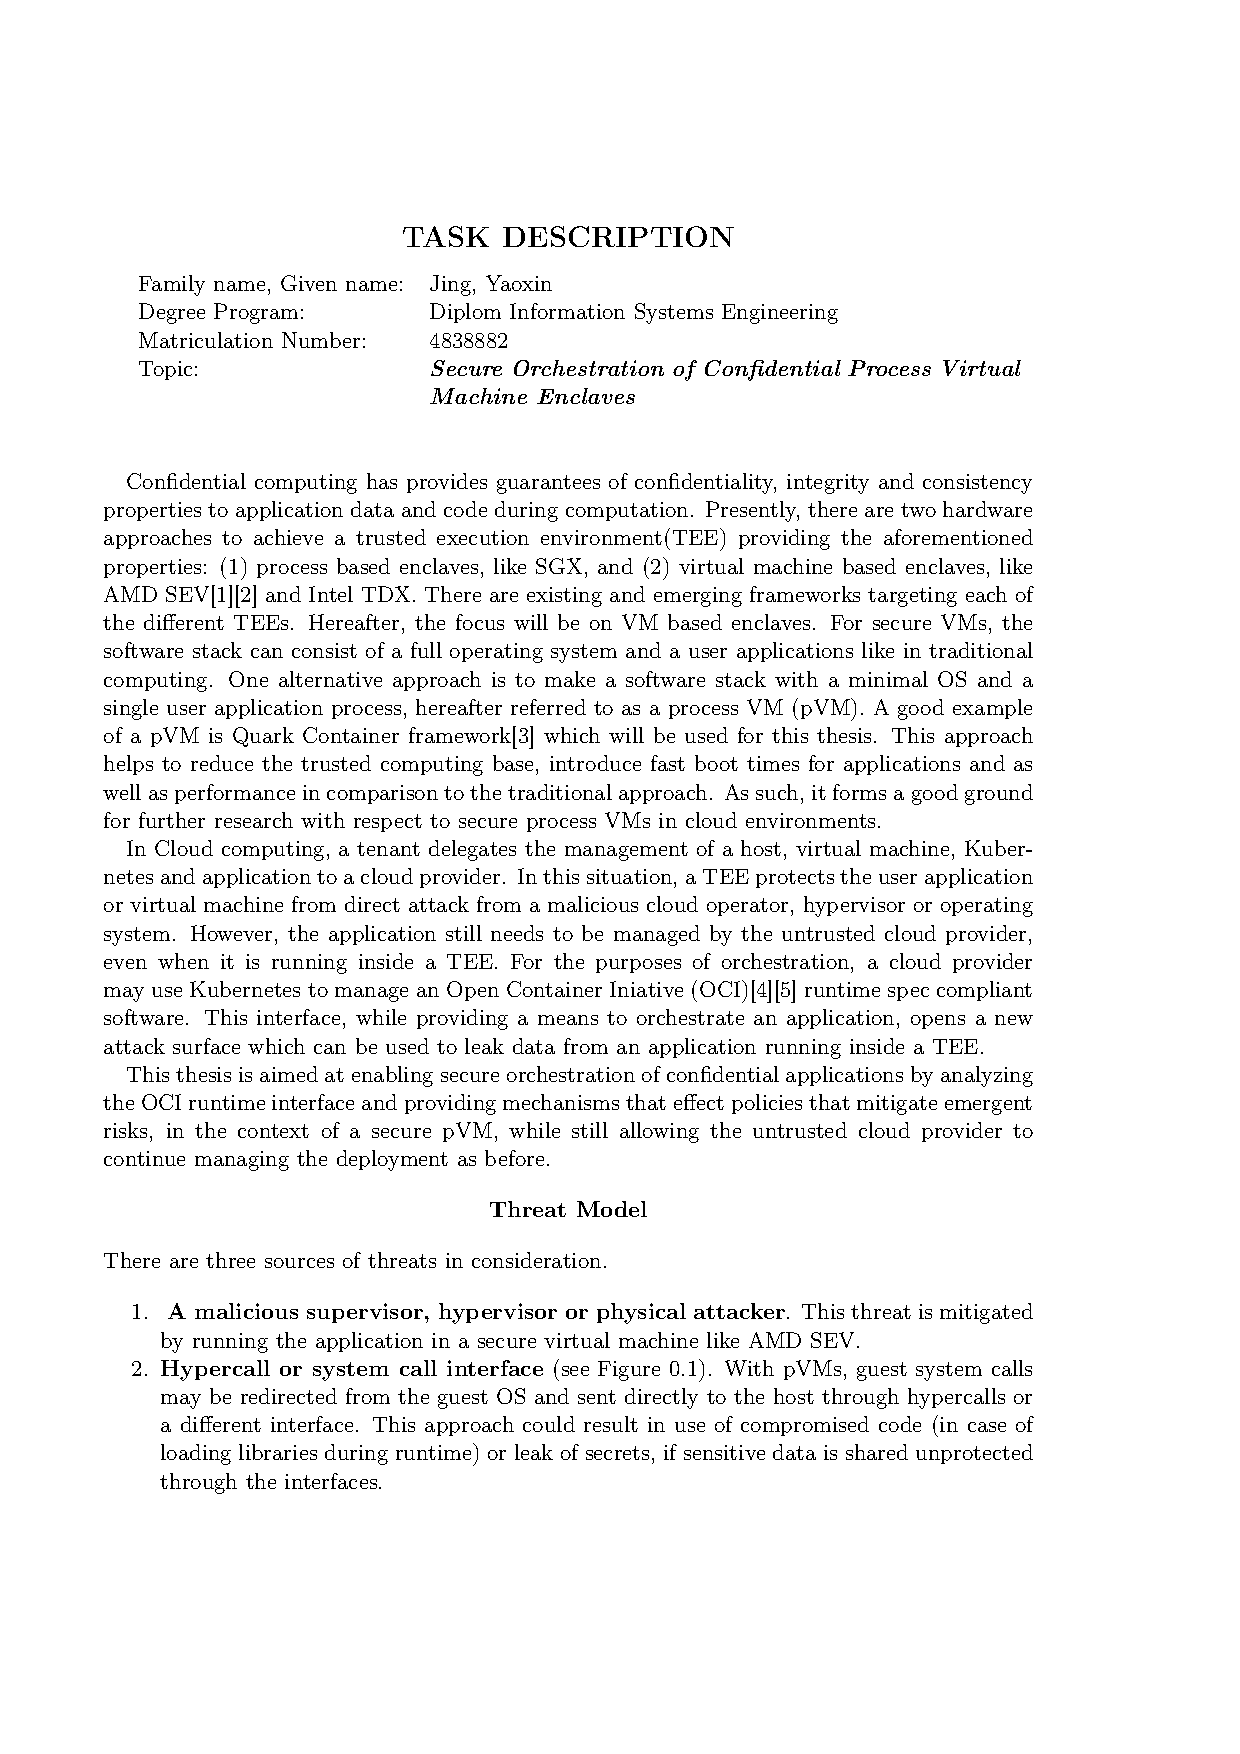
\includepdf[page=1-3]{images/yaoxin_jing_signed.pdf}
%\cleardoublepage

 
\selectlanguage{ngerman}

\section*{\vfill{} \thispagestyle{empty}
Selbständigkeitserklärung}

Hiermit versichere ich, dass ich das vorliegende Dokument selbstständig und ohne unzulässige
Hilfe Dritter verfasst habe. Es wurden keine anderen als die in diesem Dokument angegebenen
Hilfsmittel und Quellen benutzt. Die wörtlichen und sinngemäß übernommenen Zitate habe ich 
als solche kenntlich gemacht. Es waren keine weiteren Personen an der geistigen Herstellung 
des vorliegenden Dokumentes beteiligt. Mir ist bekannt, dass die Nichteinhaltung dieser
Erklärung zum nachträglichen Entzug des Hochschulabschlusses führen kann.
\bigskip{}

\noindent Dresden, den \today % \printdate % if you defined date earlier
\vspace{2.5cm}

\noindent Ziyi Fu {}
%\cleardoublepage

% NOTE: if you selected british or american above, change that here too
\selectlanguage{american}

% \begin{abstract}
% % -*- Mode: Latex -*-

%  Zusammenfassung

% Zu einer runden Arbeit gehört auch eine Zusammenfassung, die
% eigenständig einen kurzen Abriß der Arbeit gibt. Eine halbe bis ganze
% DINA4 Seite ist angemessen. Dafür läßt sich keine Gebrauchsanweisung
% geben (für irgendetwas müssen die Betreuer ja auch noch da
% sein).

%\ldots abstract \ldots

%\todo{write abstract}

Container technologies, such as Docker~\cite*{docker} and Kubernetes~\cite*{k8s}, have gained significant popularity in recent years due to the microservices trend. This technology allows tenants to quickly deploy and automate the management of applications in cloud environments. However, privacy concerns 
have hindered the popularity of cloud services in industries such as finance or healthcare~\cite*{data_privacy}~\cite*{eu_data_Privacy}. Even though novel container runtimes (e.g., kata container~\cite*{Kata-Containers}) increase the isolation level of containers dramatically by using hardware virtualization. 
It fails to ensure the confidentiality of the container's data when the host system is untrustworthy.

Trusted execution environments (\acrshort{TEE}s) provide a mechanism to protect the confidentiality and integrity of code and data running in untrusted environments. However, none of the existing TEEs are designed for secure orchestration of containers. Untrusted Kubernetes can employ the OCI runtime interface~\cite*{oci-runtime-spec} to coordinate the execution of 
TEE-protected applications and issue arbitrary commands to them. This interface enables attackers to circumvent the TEE's protection mechanisms and gain unauthorized access to the application's sensitive information.

Consequently, this thesis aims to analyze the OCI runtime interface and propose a solution for safeguarding containers from attacks from the above interface. The policy ensures the confidentiality and integrity of a container's data and code in the TEE while enabling untrusted Kubernetes\cite*{k8s} to deploy and manipulate containers as 
before. In particular, we choose the Quark framework~\cite*{quark}, a container runtime based on the process VM (\acrshort{pVM}) architecture, as a starting point for investigating container secure orchestration. In comparison, Quark offers a smaller Trusted Computing Base (\acrshort{TCB}) and substantial performance 
benefits over the traditional virtual machine-based Kata containers~\cite*{quark_performance_report}. Evaluation results demonstrate that our implementation successfully achieves the design goal, albeit resulting in a 1.48-fold increase in the \acrshort{TCB} (i.g., guest binary size). Inevitably, due to the interception and 
checking of commands from the OCI runtime interface, our implementation imposes overheads on applications.  For example, the startup time for Redis~\cite*{redis} has increased by 2.2 times, while the throughput has decreased by 22\%.
%%% Local Variables:
%%% TeX-master: "diplom"
%%% End:



% \end{abstract}

% \cleardoublepage

\tableofcontents

% \cleardoublepage


% remove this on final
% \listoftodos
% \cleardoublepage

\listoffigures
% \cleardoublepage

\listoftables

\pagenumbering{arabic}
\chapter{Introduction}
\label{sec:intro}

% Die Einleitung schreibt man zuletzt, wenn die Arbeit im Großen und
% Ganzen schon fertig ist. (Wenn man mit der Einleitung beginnt - ein
% häufiger Fehler - braucht man viel länger und wirft sie später doch
% wieder weg). Sie hat als wesentliche Aufgabe, den Kontext für die
% unterschiedlichen Klassen von Lesern herzustellen. Man muß hier die
% Leser für sich gewinnen. Das Problem, mit dem sich die Arbeit befaßt,
% sollte am Ende wenigsten in Grundzügen klar sein und dem Leser
% interessant erscheinen. Das Kapitel schließt mit einer Übersicht über
% den Rest der Arbeit. Meist braucht man mindestens 4 Seiten dafür, mehr
% als 10 Seiten liest keiner.

\todo{adopt title page}

\todo{adopt disclaimer}

\todo{write introduction}

\section{A Section}

Referencing other chapters: \ref{sec:state} \ref{sec:design}
\ref{sec:implementation} \ref{sec:evaluation} \ref{sec:futurework}
\ref{sec:conclusion}

\begin{table}[htp]
  \centering
  \begin{tabular}{lrr}
    \textbf{Name} & \textbf{Y} & \textbf{Z} \\
    \hline
    \textit{Foo} & 20,614 & \unit[23]{\%} \\
    \textit{Bar} & 9,914 & \unit[11]{\%} \\
    \textit{Foo + Bar} & 30,528 & \unit[34]{\%} \\
    \hline
    \textit{total} & 88,215 & \unit[100]{\%} \\

  \end{tabular}
  \caption[Some interesting numbers]{Various very important looking numbers and sums.}
  \label{tab:numbers}
\end{table}

More text referencing Table~\ref{tab:numbers}.

\section{Another Section}

\begin{figure}[tbp]
  \centering
  \includegraphics[width=0.8\textwidth]{images/squirrel}
  \caption[Short description]{A long description of this squirrel figure.
  Image taken from
  \url{http://commons.wikimedia.org/wiki/File:Sciurus-vulgaris_hernandeangelis_stockholm_2008-06-04.jpg}}
  \label{fig:squirrel}
\end{figure}

and Figure~\ref{fig:squirrel}.

Something with umlauts and a year/month date:


And some online resources:

\section{Yet Another Section}

\todo{add content}

\begin{figure}[tbp]
 \missingfigure{Come up with a mindblowing figure.}
 \caption{A mindblowing figure}
 \label{fig:todo}
\end{figure}

\section{Test commands}

\drops \LLinux \NOVA \QEMU
\texttt{memcpy}
A sentence about BASIC. And a correctly formatted one about ECC\@.


This thesis runs as follows:
Chapter 2 State of Art
Chapter 3 Technical Background
Chapter 4 Design and Security Analysis
Chapter 5 Implementation
Chapter 6 Evaluation
Chapter 7 Discussion

\cleardoublepage

%%% Local Variables:
%%% TeX-master: "diplom"
%%% End:

\chapter{STATE OF THE ART}
\label{sec:state}

% Hier werden zwei wesentliche Aufgaben erledigt:

% 1. Der Leser muß alles beigebracht bekommen, was er zum Verständnis
% der späteren Kapitel braucht. Insbesondere sind in unserem Fach die
% Systemvoraussetzungen zu klären, die man später benutzt. Zulässig ist
% auch, daß man hier auf Tutorials oder Ähnliches verweist, die hier auf
% dem Netz zugänglich sind.

% 2. Es muß klar werden, was anderswo zu diesem Problem gearbeitet
% wird. Insbesondere sollen natürlich die Lücken der anderen klar
% werden. Warum ist die eigene Arbeit, der eigene Ansatz wichtig, um
% hier den Stand der Technik weiterzubringen? Dieses Kapitel wird von
% vielen Lesern übergangen (nicht aber vom Gutachter ;-), auch später
% bei Veröffentlichungen ist "Related Work" eine wichtige Sache.

% Viele Leser stellen dann später fest, daß sie einige der Grundlagen
% doch brauchen und blättern zurück. Deshalb ist es gut,
% Rückwärtsverweise in späteren Kapiteln zu haben, und zwar so, daß man
% die Abschnitte, auf die verwiesen wird, auch für sich lesen
% kann. Diese Kapitel kann relativ lang werden, je größer der Kontext
% der Arbeit, desto länger. Es lohnt sich auch! Den Text kann man unter
% Umständen wiederverwenden, indem man ihn als "Tutorial" zu einem
% Gebiet auch dem Netz zugänglich macht.

% Dadurch gewinnt man manchmal wertvolle Hinweise von Kollegen. Dieses
% Kapitel wird in der Regel zuerst geschrieben und ist das Einfachste
% (oder das Schwerste weil erste).

%\ldots state of the art \ldots

%\todo{write state}

\section{vm-cc}
\section{microvm-cc/kata-cc*1}
\section{enclave-cc/SCONE}
\section{process-like vm-cc/Confidentail quark}
\section{Compare vm-cc /microvm-cc/enclave-cc then say pico vm cc solution is future}
\cleardoublepage

%%% Local Variables:
%%% TeX-master: "diplom"
%%% End:

% \chapter{Technical Background}
\label{sec:state}

% Hier werden zwei wesentliche Aufgaben erledigt:

% 1. Der Leser muß alles beigebracht bekommen, was er zum Verständnis
% der späteren Kapitel braucht. Insbesondere sind in unserem Fach die
% Systemvoraussetzungen zu klären, die man später benutzt. Zulässig ist
% auch, daß man hier auf Tutorials oder Ähnliches verweist, die hier auf
% dem Netz zugänglich sind.

% 2. Es muß klar werden, was anderswo zu diesem Problem gearbeitet
% wird. Insbesondere sollen natürlich die Lücken der anderen klar
% werden. Warum ist die eigene Arbeit, der eigene Ansatz wichtig, um
% hier den Stand der Technik weiterzubringen? Dieses Kapitel wird von
% vielen Lesern übergangen (nicht aber vom Gutachter ;-), auch später
% bei Veröffentlichungen ist "Related Work" eine wichtige Sache.

% Viele Leser stellen dann später fest, daß sie einige der Grundlagen
% doch brauchen und blättern zurück. Deshalb ist es gut,
% Rückwärtsverweise in späteren Kapiteln zu haben, und zwar so, daß man
% die Abschnitte, auf die verwiesen wird, auch für sich lesen
% kann. Diese Kapitel kann relativ lang werden, je größer der Kontext
% der Arbeit, desto länger. Es lohnt sich auch! Den Text kann man unter
% Umständen wiederverwenden, indem man ihn als "Tutorial" zu einem
% Gebiet auch dem Netz zugänglich macht.

% Dadurch gewinnt man manchmal wertvolle Hinweise von Kollegen. Dieses
% Kapitel wird in der Regel zuerst geschrieben und ist das Einfachste
% (oder das Schwerste weil erste).

%\ldots state of the art \ldots

%\todo{write state}
This chapter offers background knowledge for all the content and topics covered in the thesis. The reader is assumed to understand operating systems, Kubernetes\cite*{k8s}, and confidential computing. Nonetheless, it provides a concise overview of essential terms and concepts to facilitate the reader's 
comprehension of subsequent chapters.

\section{Kubernetes and runtime communication interface}
\label{sec:k8s}
Kubernetes~\cite*{k8s} is a tool for managing and orchestrating containers. It comprises at least one master node and multiple worker nodes. The master node handles global decision-making, scheduling, and managing cluster events. As shown in Figure~\ref{fig:k8s}, 
the master node hosts an API server that provides users with an interface to manage and control the cluster. Users can submit requests to create or update Kubernetes objects like pods. A pod represents the smallest deployment unit in Kubernetes, which may contain multiple containers sharing network 
and storage resources. Moreover, each worker node runs a Kubelet, a daemon responsible for processing requests from the master node and executing services on the worker node. When handling container creation and image management requests, Kubelet invokes a high-level container runtime like 
Containerd~\cite*{containerd} or CRI-O~\cite*{cri-o}.These high-level runtimes take charge of managing the container lifecycle and images while delegating pod creation and 
deletion to lower-level OCI-compliant runtimes such as Kata~\cite*{Kata-Containers}, Quark~\cite*{quark}, RunC~\cite*{runc}, etc.
\begin{figure}[htp]
  \centering
  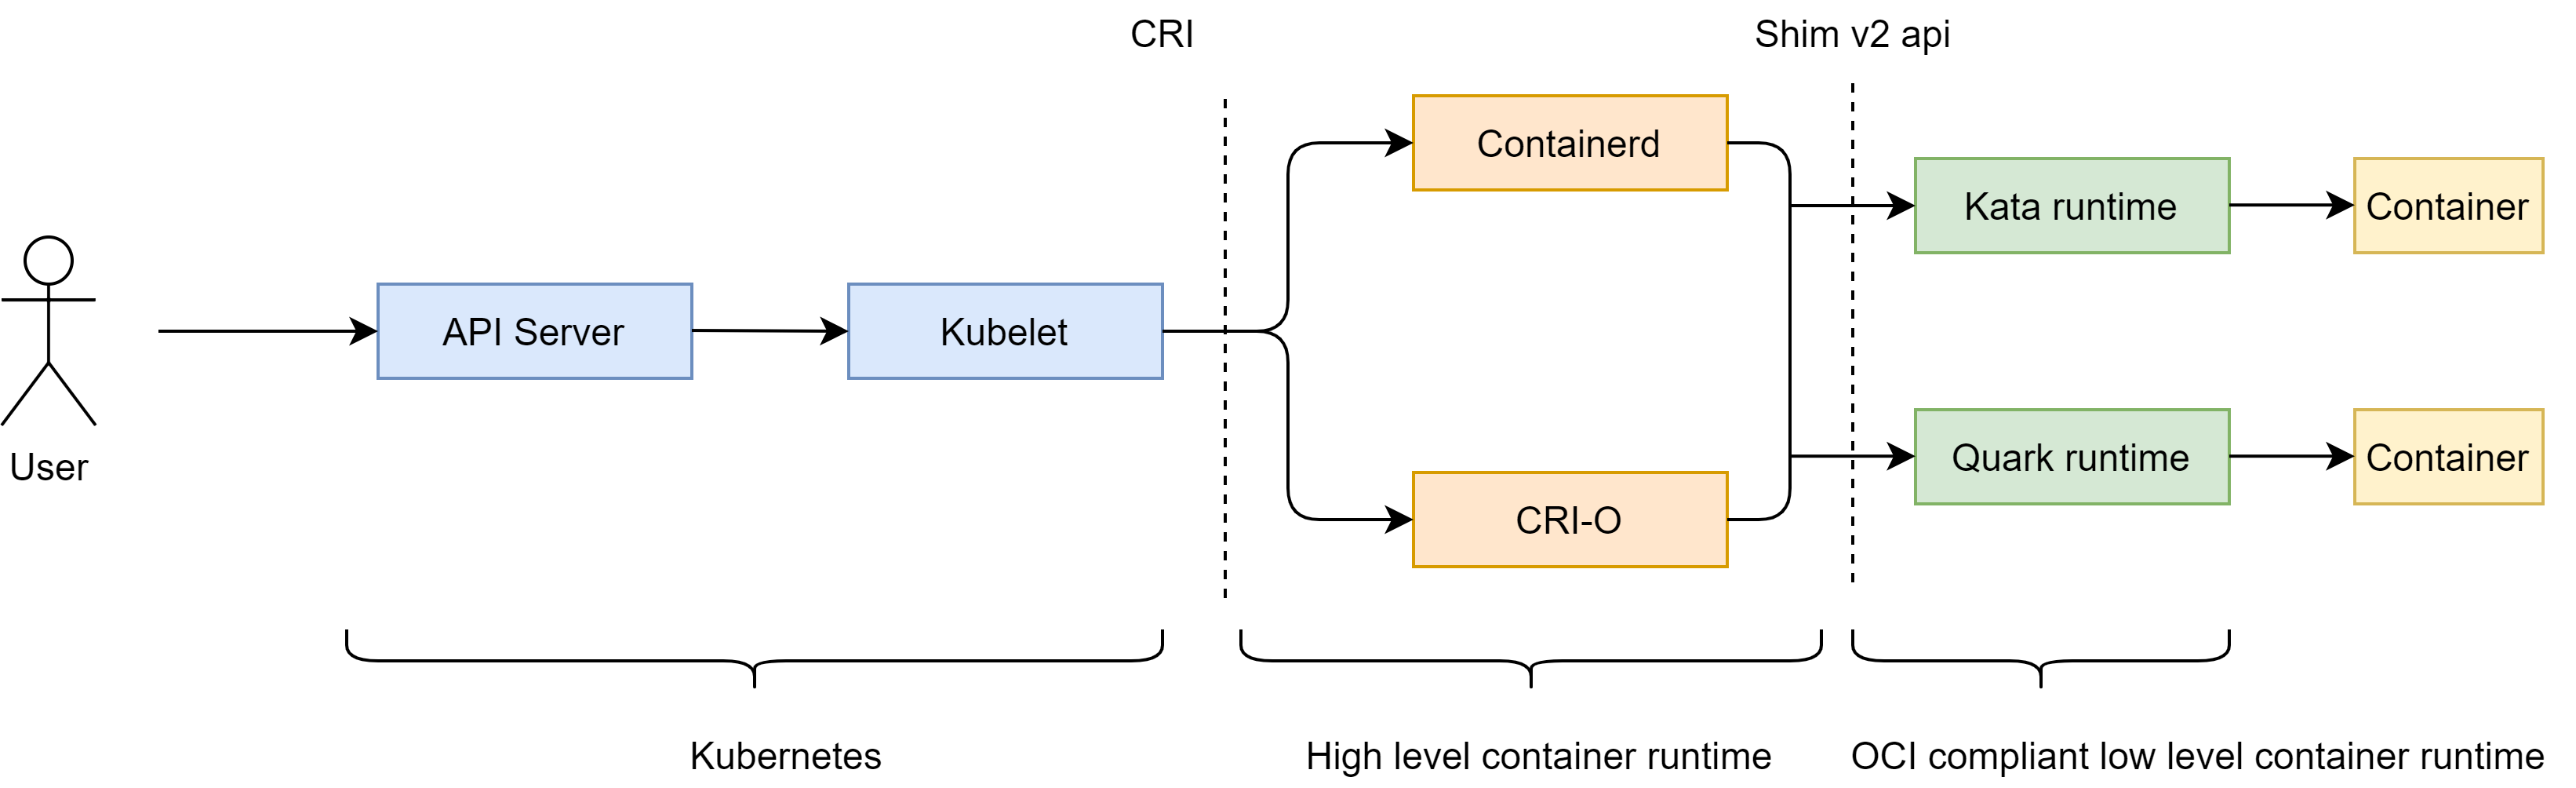
\includegraphics[width=0.8\textwidth]{images/k8s.PNG}
  \caption[Kubernetes architecture and runtime communication interface]{Kubernetes architecture and runtime communication interface}
  \label{fig:k8s}
\end{figure}

Standardized communication interfaces have been defined among the components in Figure~\ref{fig:k8s} for compatibility and scalability. The Kubelet utilizes the CRI interface~\cite*{cri-interface} to access services offered by the high-level runtime. Within the CRI, two gRPC interfaces are defined: 
the \texttt{ImageService} interface, responsible for managing images, and the \texttt{RuntimeService} interface, which manages containers and pods. Any high-level runtime integrated into the Kubernetes ecosystem should implement the CRI interface. In addition, high-level runtimes support low-level 
runtimes that implement the shim interface~\cite*{shim_v2, cri0_shim_v2}. In Containerd, this interface is known as the \texttt{shim v2 API}~\cite*{shim_v2}, encompassing multiple ttrpc endpoints. It aims to abstract the implementation details of the low-level runtime and facilitate 
communication between higher-level runtimes and various lower-level runtimes.


\section{OCI runtime specification}
\label{sec:back_oci_runtime_spec}
To ensure container portability and compatibility across runtimes, the Open Container Initiative (OCI) has introduced the OCI runtime specification~\cite*{oci-runtime-spec}. This specification outlines the procedure for low-level container runtimes to create and execute containers based on an 
application bundle. The high-level container runtime generates the application bundle from an image. It contains the container's root file system and a configuration file. This bundle is transferred to the low-level runtime during the container creation phase. 
The low-level runtime utilizes the metadata provided in the configuration file to create and configure the container. This metadata includes the following information: a process configuration, metadata defining the container root file system, and mount information. The process configuration contains 
the necessary metadata for creating the application or EXEC process, including environment variables, program argument list (e.g., ["cat", "/"]), STDIO type, etc. Mount information indicates the files or filesystems that should be mounted to the container's root filesystem. This may include 
Kubernetes secrets, Kubernetes configuration files, and volumes~\cite*{k8s}. Additionally, on Linux platforms, the configuration file includes settings for container security and hooks. These hooks are executable and executed by low-level container runtime at 
different stages of the container lifecycle (Figure~\ref{fig:Container_Lifecycle_state}).
\begin{figure}[htp]
  \centering
  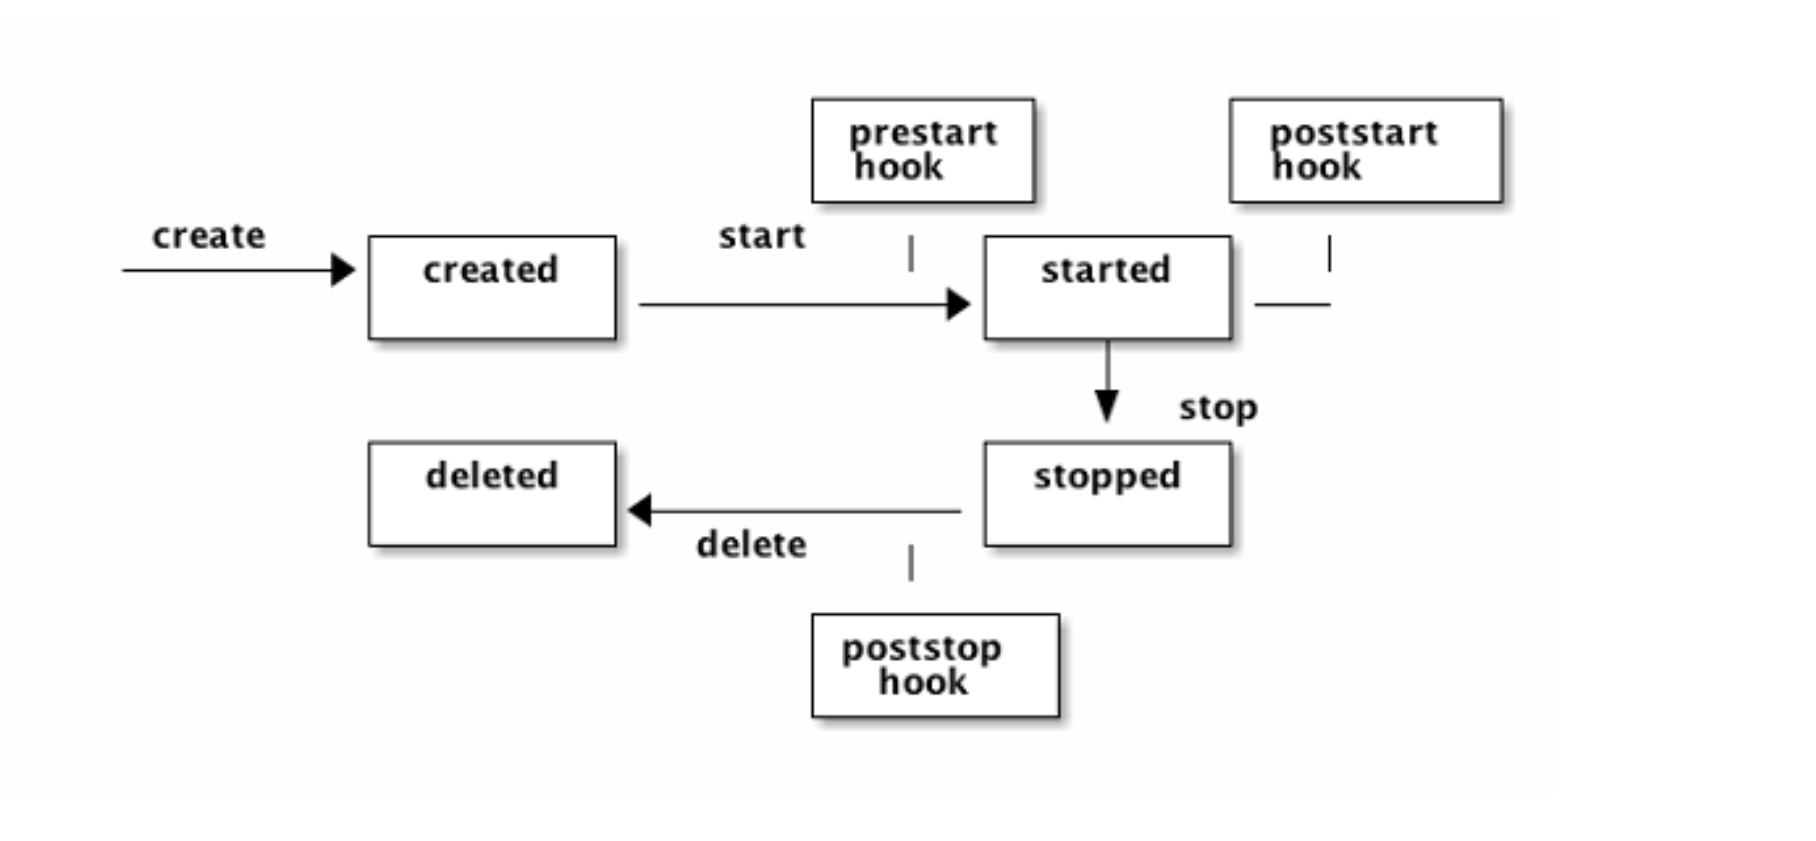
\includegraphics[width=0.8\textwidth]{images/Container_Lifecycle_state.PNG}
  \caption[Overview of container lifecycle]{Overview of container lifecycle from \cite*{oci_Lifecycle}}
  \label{fig:Container_Lifecycle_state}
\end{figure}

\section{Kata containers}
\label{sec:Kata}

Kata containers is an OCI-compliant low-level container runtime derived from combining two projects: Clear Containers and Hyper RunV~\cite*{Kata-Containers}. It runs containers in an ultra-lightweight virtual machine. This architecture preserves the speed of containers and utilizes 
hardware virtualization technology to enhance container isolation~\cite*{Kata-Containers}.
\begin{figure}[htp]
  \centering
  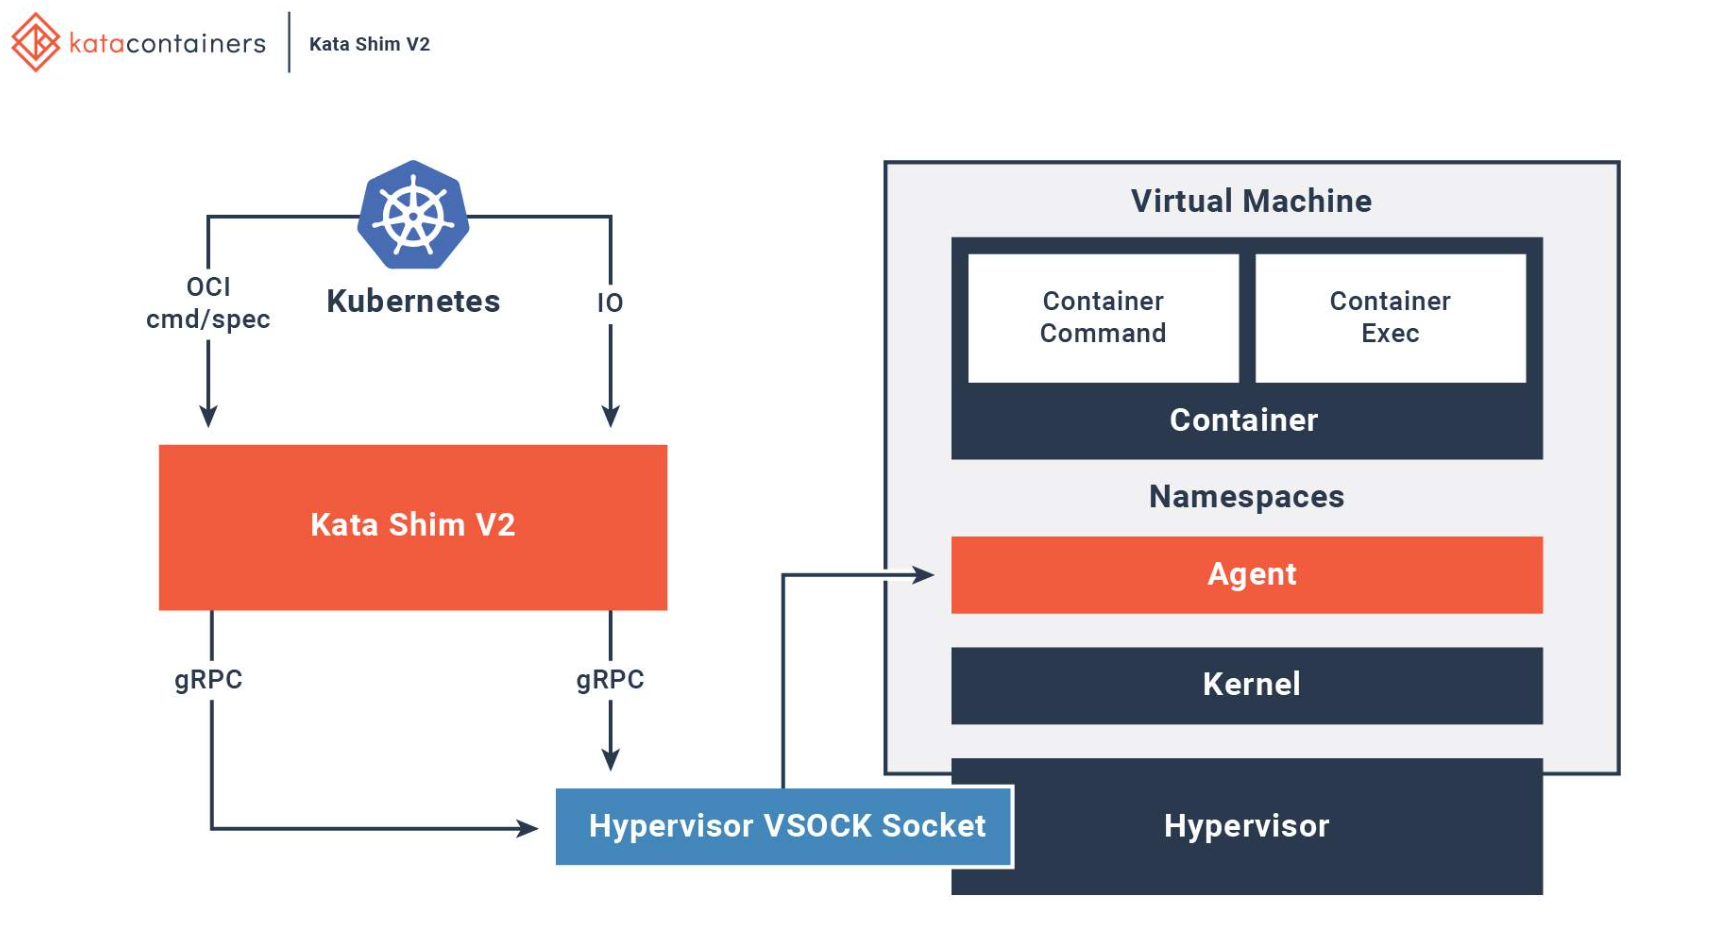
\includegraphics[width=0.6\textwidth]{images/kata.PNG}
  \caption[Kata containers architecture]{Kata containers architecture from~\cite*{Kata-Containers} }
  \label{fig:kata}
\end{figure}
Figure~\ref{fig:kata} presents the latest architecture (version 2.0) of Kata containers~\cite*{Kata_arch}. It consists of four elements: Kata Shim v2, hypervisor, guest kernel, and Kata agent. Kata shim v2 is a merging of multiple components in version 1.0, including the Kata shim, 
the Kata proxy, and the OCI-compliant Kata runtime~\cite*{Kata_arch}. It implements the \texttt{shim v2 API}~\cite*{shim_v2}. Therefore, Containerd~\cite*{containerd} can issue commands to it.  The Kata agent is a daemon running inside the virtual machine. It is responsible for handling commands 
from Kata shim v2 and managing the containers within the VM. Communication between Kata shim v2 and the Kata agent is facilitated through the VM's \texttt{VIRTIO} or \texttt{VSOCK} interface and the gRPC protocol~\cite*{Kata_arch}. Furthermore, the 
Kata containers utilize a highly optimized hypervisor and guest kernel that strips off unnecessary modules to achieve a low boot time and small memory footprint~\cite*{8939164}.


\section{Quark containers}
\label{sec:Quark}
Quark containers~\cite*{quark} is an OCI-compliant container runtime written in the Rust language. Similar to Kata containers~\cite*{Kata-Containers}, it also runs the containers in the VM. 
The difference is that Quark uses an application kernel (also known as the forward kernel) as a guest OS. It implements some system calls and forwards others to the host. Compared to the Kata containers, its guest kernel is smaller since it reuse many services the host provides, eliminating unnecessary code.
Consequently, Quark has a smaller memory footprint and faster startup time~\cite*{quark_performance_report}. Moreover, Quark has developed the Ucall and Qcall interfaces to facilitate communication with the host. This approach efficiently avoids expensive VM exits when 
forwarding system calls to the host.

\begin{figure}[htp]
  \centering
  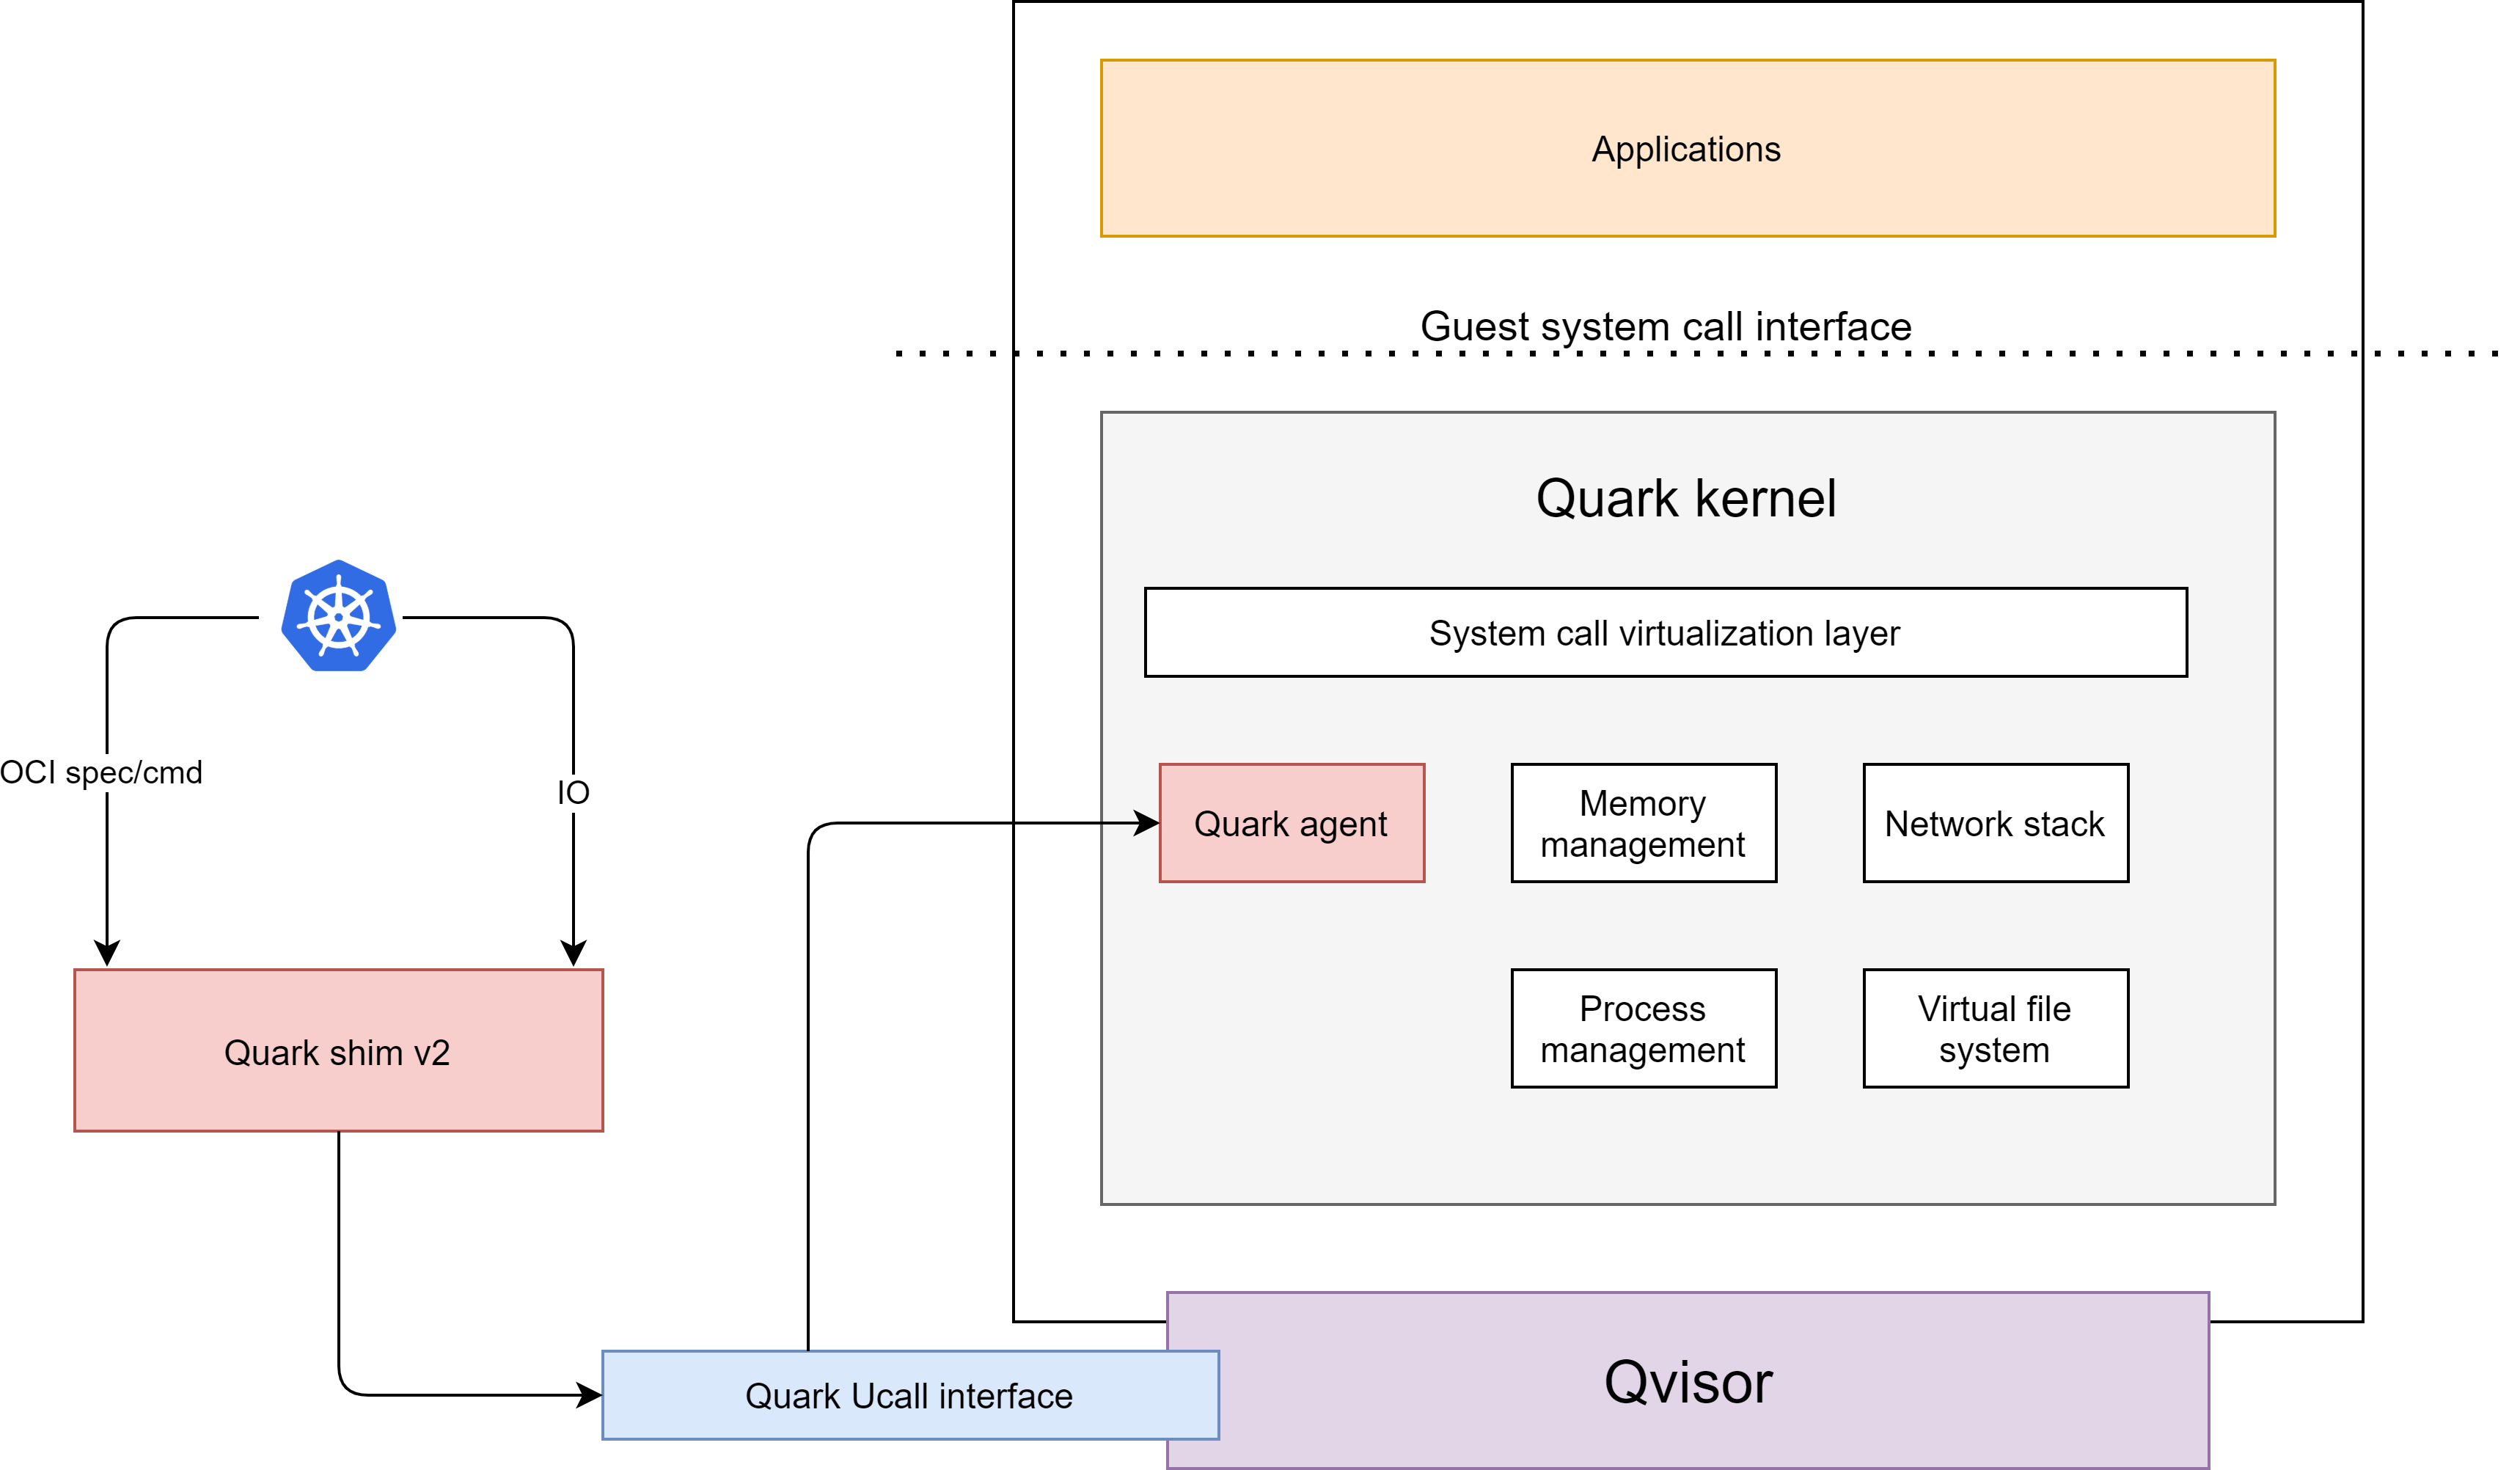
\includegraphics[width=0.6\textwidth]{images/QUARK_ARCH.PNG}
  \caption[Quark containers architecture]{Quark containers architecture}
  \label{fig:QUARK_ARCH}
\end{figure}


The architecture of the Quark container, as depicted in Figure~\ref{fig:QUARK_ARCH}, comprises three elements: Quark shim, Qvisor, and Qkernel. Similarly to the Kata shim, the Quark shim is an OCI-compliant ttrpc server implemented following the \texttt{shim v2 API}~\cite*{shim_v2}. As a 
result, it can execute commands from Containerd~\cite*{containerd}. These commands may include invoking Qvisor to create lightweight virtual machines for running containers with Qkernel as the guest OS. Qvisor is a virtual machine manager similar to QEMU. It utilizes the KVM API to create and 
manage VMs. Qkernel, on the other hand, is a minimized application kernel that contains only the necessary code. It employs the host service to implement process management, memory management, file system, and network stack. 
In addition, Qkernel implements most of the Linux system calls, which can be triggered by guest processes using the x86 \texttt{SYSCALL} instruction. To accept the request from the Quark shim, Qkernel implements a socket server called Quark agent. It uses Hypercall, Ucall, and Qcall interfaces to 
communicate with Quark shim. Unlike the Kata agent, which operates as a user space process, the Quark agent is integrated within the Qkernel, and its code is part of the Qkernel (guest kernel) binary.



\begin{figure}[htp]
  \centering
  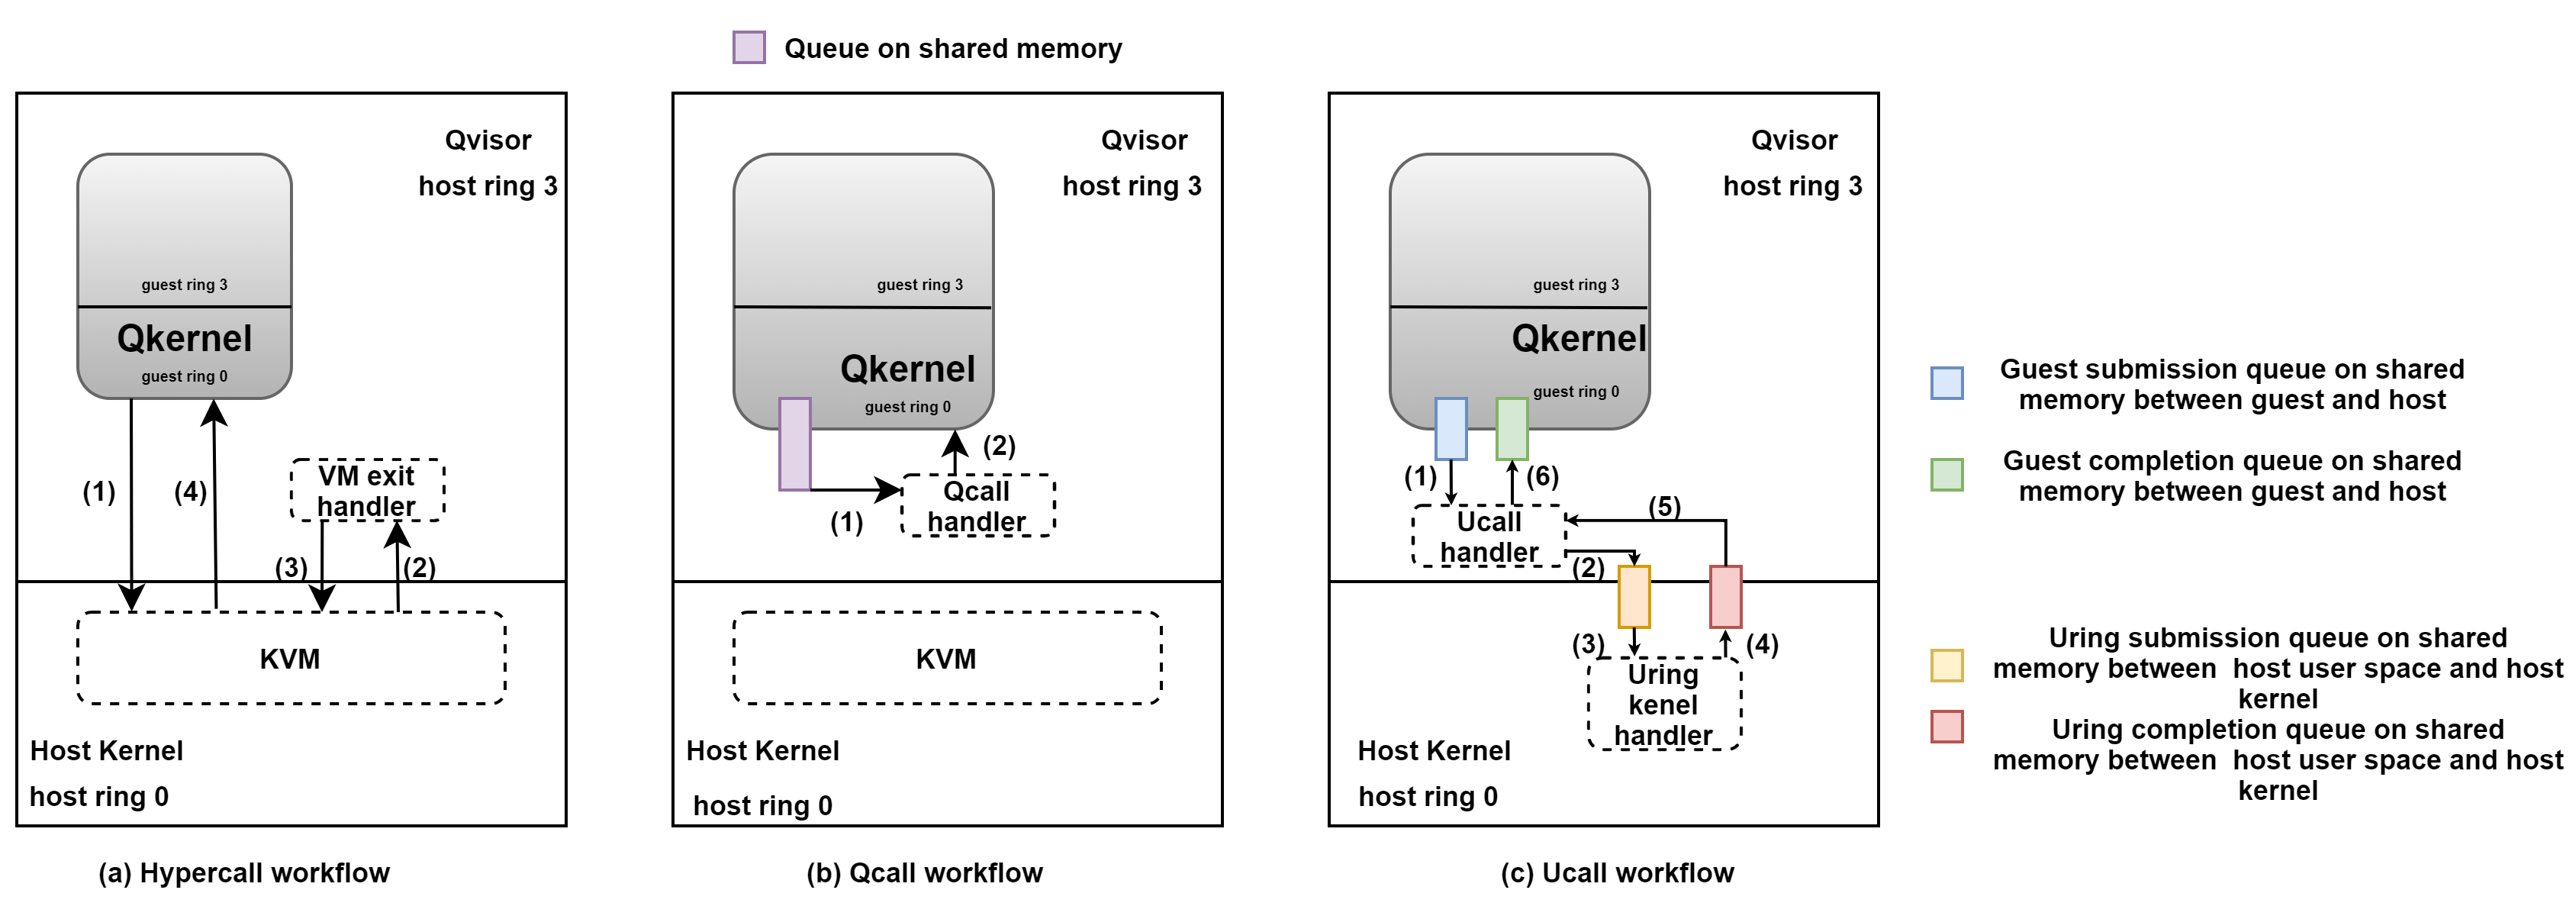
\includegraphics[width=1\textwidth]{images/hypercall_qcall_ucall.png}
  \caption[Workflow of Hypercall, Qcall, and Ucall]{Workflow of Hypercall, Qcall, and Ucall}
  \label{fig:hypercall_qcall_ucall}
\end{figure}


The workflow of Hypercall, Qcall, and Ucall is depicted in Figure~\ref{fig:hypercall_qcall_ucall}. Hypercall serves as the traditional mechanism for guests to communicate with the Virtual Machine Monitor (VMM). Qkenrel employs Hypercall to access services in Qvisor, like file opening and IO 
initialization. Figure~\ref{fig:hypercall_qcall_ucall} (a) illustrates the workflow of Hypercall. Upon triggering Hypercall, the CPU mode is changed from the guest ring 0  to the host ring 0. Subsequently, the KVM examines the Virtual Machine Control Block to determine the reason for the VM exit and 
forwards the Hypercall to the Qvisor running in host ring 3. Following the processing of the Hypercall, the Qvisor requests the KVM to resume guest execution.

Executing a Hypercall incurs significant overhead due to multiple world switches. As such, Quark offers an asynchronous mechanism known as Qcall as an alternative approach for communicating with Qvisor. As depicted in Figure~\ref{fig:hypercall_qcall_ucall} (b), this mechanism consists of a 
shared memory queue between the Qkernel and the Qvisor and an IO thread in Qvisor. The shared queue facilitates the transfer of requests from Qkernel to Qvisor. The IO thread is responsible for retrieving the requests from the queue and notifying or awakening the Qkernel thread once the Qvisor 
completes the request. In summary, this mechanism allows Qkernel to access services in Qvisor asynchronously, eliminating the need for VM exit. 

The host operating system is responsible for performing IO read and write operations on physical devices. Therefore, Quark introduces the Ucall mechanism for communicating with the host kernel. This mechanism utilizes the Linux \texttt{io\_uring}~\cite*{io_uring} and shared queues between 
Qvisor and Qkernel. It supports both synchronous and asynchronous IO operations. Figure~\ref{fig:hypercall_qcall_ucall} (c) explains the workflow of this mechanism. Initially, a Qkernel thread submits an IO request to the guest submission queue (Figure ~\ref{fig:hypercall_qcall_ucall} (c) step 1). 
Subsequently, the Qvisor Ucall handler copies the request to the uring submission queue (Figure~\ref{fig:hypercall_qcall_ucall} (c) step 2). Once the uring kernel handler completes processing the IO request, it places the result into the uring completion 
queue (Figure~\ref{fig:hypercall_qcall_ucall} (c) step 3, 4). The result includes a \emph{user\_data}, which is submitted with the initial IO request and contains information about the Qkernel thread. The Qvisor Ucall handler can use this information to notify the corresponding Qkernel thread. 
Note that the notification occurs after the IO processing result has been copied to the guest completion queue (Figure~\ref{fig:hypercall_qcall_ucall} (c) step 5, 6).

\section{Trusted Execution Environment}

The hardware-based~\acrshort{TEE} establishes tamper-proof computing environments that ensure the confidentiality and integrity of data. It safeguards applications' private sensitive code and data against co-located attacks through verifiable boot, runtime isolation, trusted IO, and 
secure storage~\cite*{Hardware-supported-TEE}. This security guarantee relays on hardware. Consequently, compromising privileged software (e.g., operating system and hypervisor) does not diminish the~\acrshort{TEE}'s capacity to protect security-sensitive appliances ~\cite*{7345265}.


Hardware-based~\acrshort{TEE} models can be categorized into two types: virtual machine-based~\acrshort{TEE} and process-based~\acrshort{TEE}~\cite*{10.3389/fcomp.2022.930741}. Examples of virtual machine-based~\acrshort{TEE}s include Intel TDX~\cite*{Intel_tdx_whitepaper} and AMD SEV-SNP~\cite*{SEV_SNP_white_book}, whereas 
Intel SGX~\cite*{INTEL_SGX} is the most famous process-based~\acrshort{TEE}. While Intel SGX has a smaller~\acrshort{TCB}, splitting an application into trusted and untrusted parts results in a degraded user experience. In contrast, VM-based~\acrshort{TEE}s enable the execution of programs without modification. However, this approach increases the 
\acrshort{TCB}, making it more susceptible to attacks~\cite*{Execution_Environment_landscape}.

The following two sections provide an overview of VM-based~\acrshort{TEE}. The AMD SEV-SNP and Intel TDX are chosen as examples because they will likely be widely used. An explanation of process-based~\acrshort{TEE}s is beyond the scope of this thesis. For further details on the process-based~\acrshort{TEE}, 
please refer to~\cite*{cryptoeprint:2016/086, 10.1145/2487726.2488370}.


\subsection{AMD SEV-SNP}

AMD SEV-SNP~\cite*{SEV_SNP_white_book} is AMD's latest virtual machine-based~\acrshort{TEE} solution. It retains the features of its predecessors, AMD SEV~\cite*{sev} and AMD SEV-ES~\cite*{sev_es}, namely virtual machine memory encryption, register state protection, and further adds integrity protection for 
encrypted memory.


AMD SEV-SNP utilizes encryption to protect the memory of a virtual machine. When a service running in an \acrshort{CVM} accesses memory, the AES-128 encryption engine transparently encrypts or decrypts the memory using a memory encryption key~\cite*{snp_Explained}.  This key is unique for each 
VM and securely stored in the AMD secure processor (~\acrshort{AMD SP}) to prevent unauthorized access. Consequently, untrusted entities can only read the ciphertext on the VM memory. To enable memory page sharing between \acrshort{CVM}s, or between \acrshort{CVM}s and the hypervisor, SEV-SNP introduces a new 
control bit known as the "C-bit" in the page table entry~\cite*{SEV_SNP_white_book}. This allows \acrshort{CVM}s to determine which pages should be encrypted. Furthermore, SEV-SNP introduces the Reverse Map Table (RMP) to protect the integrity of VM memory~\cite*{SEV_SNP_white_book}. 
RMP records the ownership of pages and ensures that each physical page is owned by only one entity. In this case, only the page owner can modify the page content



\begin{figure}[htp]
  \centering
  \begin{subfigure}[b]{0.65\textwidth}
      \centering
      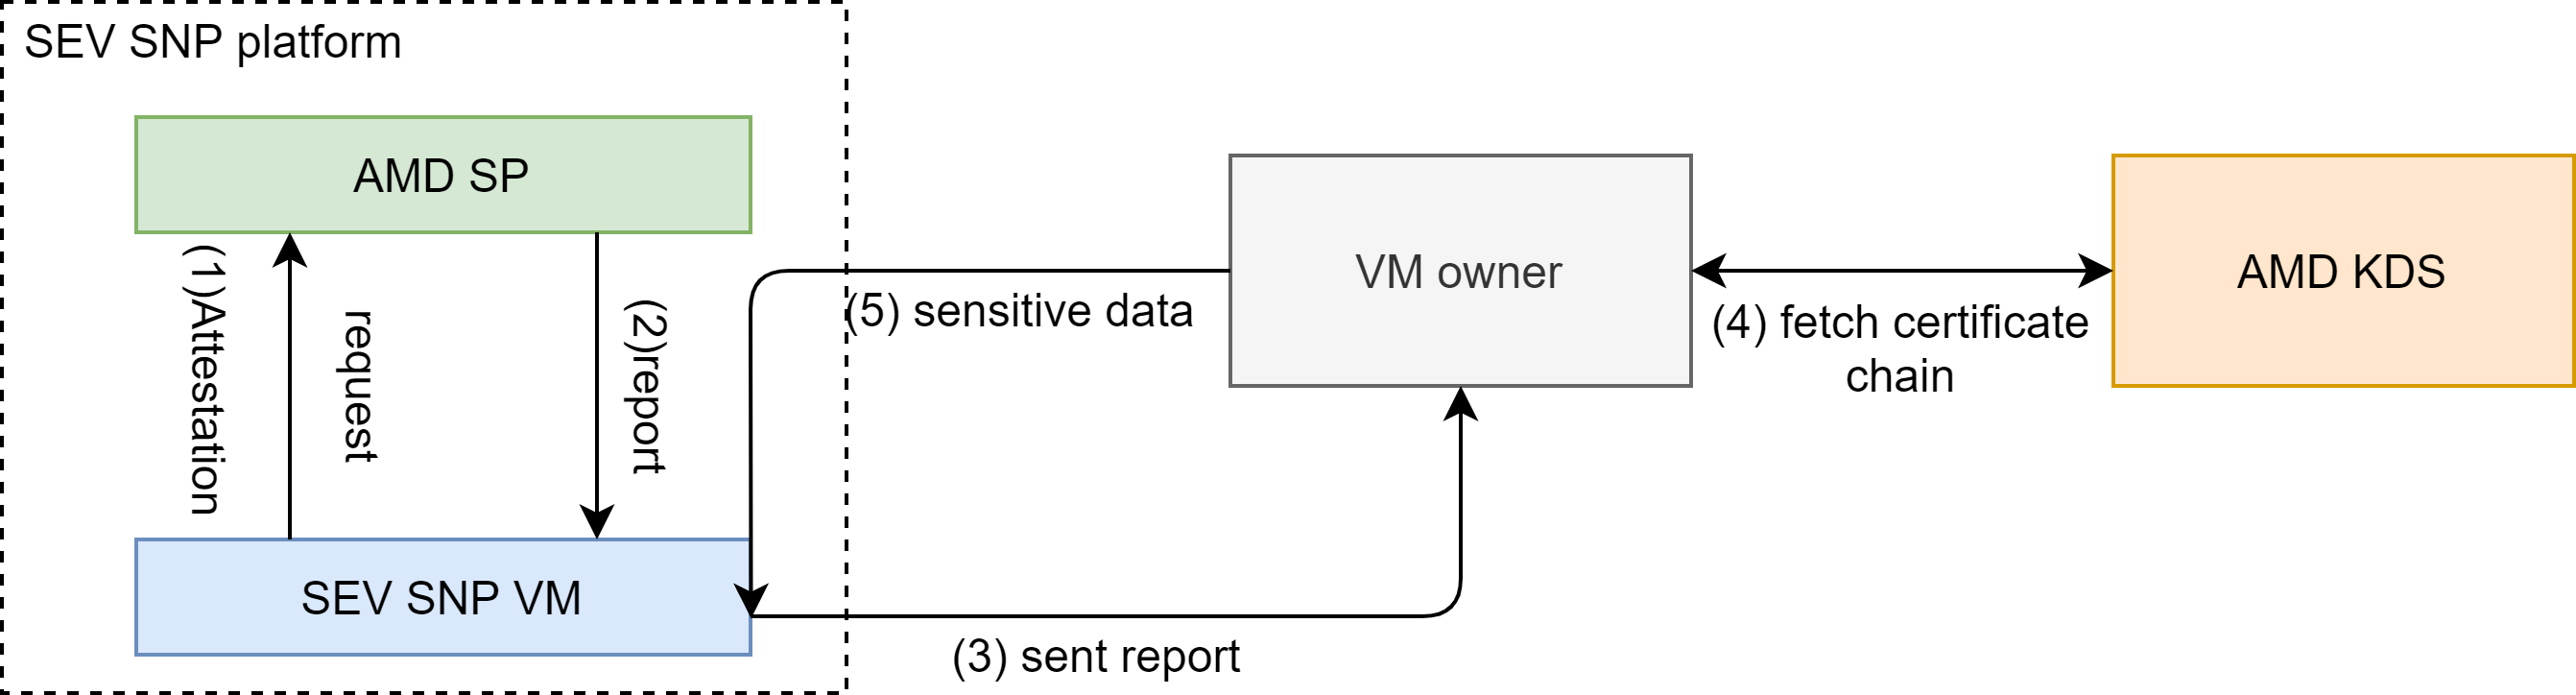
\includegraphics[width=\textwidth]{images/amd_attestation_workflow.PNG}
      \caption{Attestation workflow}
      \label{fig:amd_attestation_workflow}
  \end{subfigure}
  \hfill
  \begin{subfigure}[b]{0.3\textwidth}
      \centering
      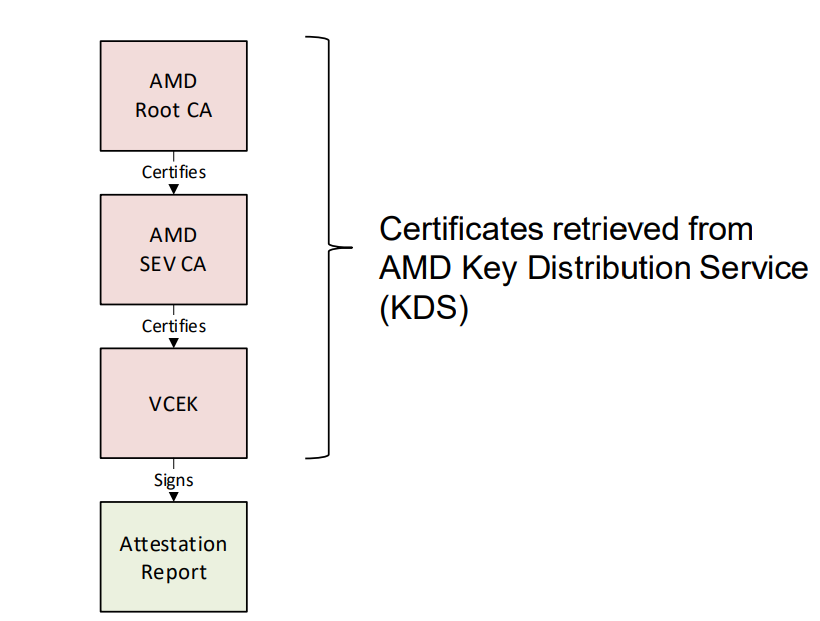
\includegraphics[width=\textwidth]{images/amd_snp_certificate_chain.PNG}
      \caption{Certificate chain (Figure from~\cite*{amd_Sev_snp_ppt})}
      \label{fig:amd_snp_certificate_chain}
  \end{subfigure}
  \hfill
     \caption[AMD SEV-SNP remote attestation]{AMD SEV-SNP remote attestation}
     \label{fig:amd_snp_atteation}
\end{figure}

SEV-SNP also supports remote attestation, which allows the \acrshort{CVM} owner to verify the authenticity of the VM. Unlike its predecessor, SEV-SNP enables \acrshort{CVM}s to obtain the attestation report from ~\acrshort{AMD SP} at runtime. The communication between the \acrshort{CVM} and~\acrshort{AMD SP} 
is facilitated by the SEV-SNP guest messages protocol~\cite*{snp_firmware, amd_sev_summarize}. A brief description of the protocol can also be found in Section~\ref{subsec:impl_Attestation_driver}.  The workflow for remote attestation is shown in Figure~\ref{fig:amd_snp_atteation} (a). 
The \acrshort{CVM} first utilizes the SEV-SNP guest messages protocol to request a report from the~\acrshort{AMD SP}. The report is signed using the Versioned Chip Endorsement Key (VCEK) and contains details such as the~\acrshort{AMD SP}'s measurement of the VM boot process, the~\acrshort{AMD SP} 
firmware version, and custom data~\cite*{snp_firmware}. The~\acrshort{VCEK} is unique to each AMD platform because it is derived from platform-specific secrets and TCB versions~\cite*{snp_firmware}. Once the \acrshort{CVM} owner receives the report,  they can utilize the \texttt{CHIP\_ID} and \texttt{TSB} fields in the report to 
retrieve a certificate chain (Figure~\ref{fig:amd_snp_atteation} (b)) from the AMD Key Distribution Center~\cite*{amd_sev_summarize}. The certificate chain can be used to verify the signature of the report. Subsequently, by examining the remaining fields of the report, the \acrshort{CVM} owner 
can determine whether the \acrshort{CVM} is genuine.

\subsection{Intel TDX}
\label{subsec:tdx}

Intel TDX~\cite*{Intel_tdx_whitepaper} is a virtual machine-based~\acrshort{TEE} solution. It introduces a new CPU mode called Secure Arbitration Mode (SEAM). As shown in Figure~\ref{fig:td_arch}, the TDX module and all \acrshort{CVM}s (TDs) run in this mode. It provides an 
isolated execution environment for TDs so that privileged software (e.g., hypervisor) running in other modes cannot access the TDs' register and memory. The TDX module manages the TDs and offers an interface for the hypervisor to send instructions to the TDs. The TDX module can verify these instructions against a security policy to ensure the TDs are correctly operated.

\begin{figure}[htp]
  \centering
  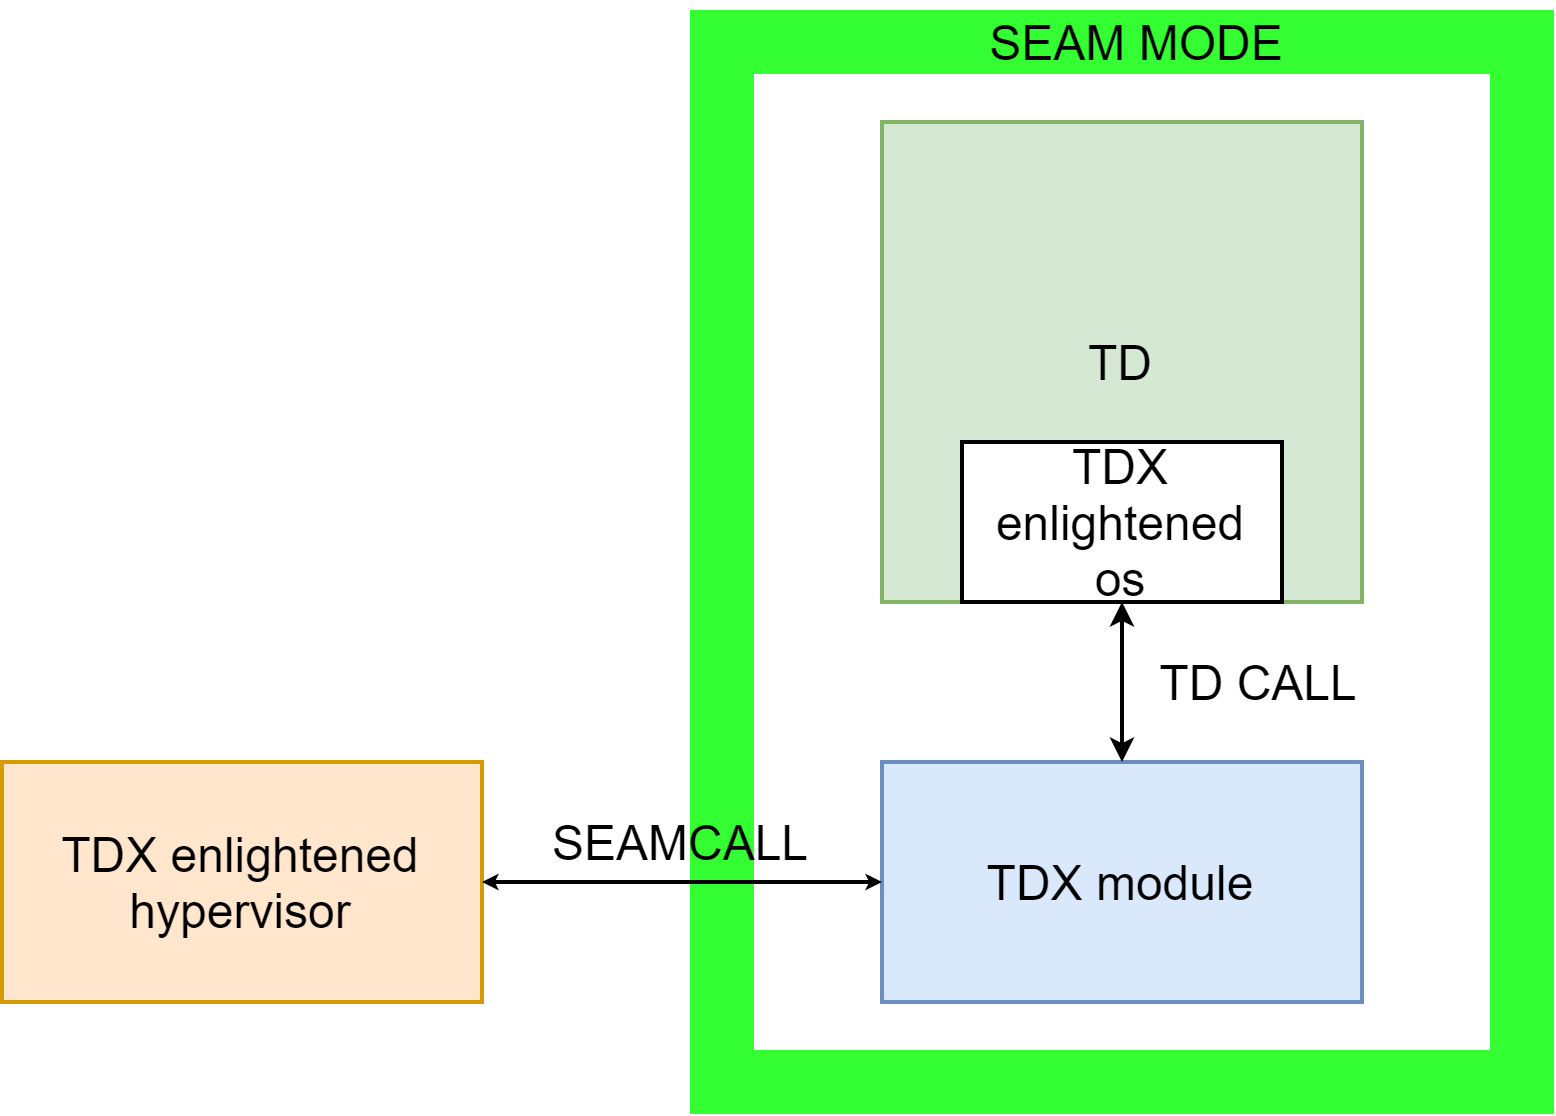
\includegraphics[width=0.4\textwidth]{images/td_arch.png}
  \caption[TDX architecture]{TDX architecture}
  \label{fig:td_arch}
\end{figure}


TDX also supports shared memory to facilitate communication between TDs or TD and untrusted entities like hypervisors. Like the SEV-SNP, each TD divides its memory into private and shared. External entities can access TD's shared memory in plaintext. This mechanism is implemented by introducing a 
new bit called the shared bit in the Guest Physical Address (GPA) and two EPTs, namely secure EPT and shared EPT~\cite*{Intel_tdx_whitepaper}. TD can use the shared bit to determine whether the Guest's Physical Address (GPA) corresponds to shared memory. The secure EPT and shared EPT are 
responsible for converting private/shared GPAs to physical addresses. Note that only the private pages are encrypted using a TD's private key ~\cite*{Intel_tdx_whitepaper}. Additionally, the Intel TDX also supports memory integrity protection. As~\cite*{kollendageneral} stated, the protection is 
achieved by \enquote{including a 1-bit TD identifier for each cache line and optionally a 28-bit message authentication code (MAC) that includes the 1-bit identifier to ensure that any unauthorized changes to the memory are detected.}


\begin{figure}[htp]
  \centering
  \begin{subfigure}[b]{0.65\textwidth}
      \centering
      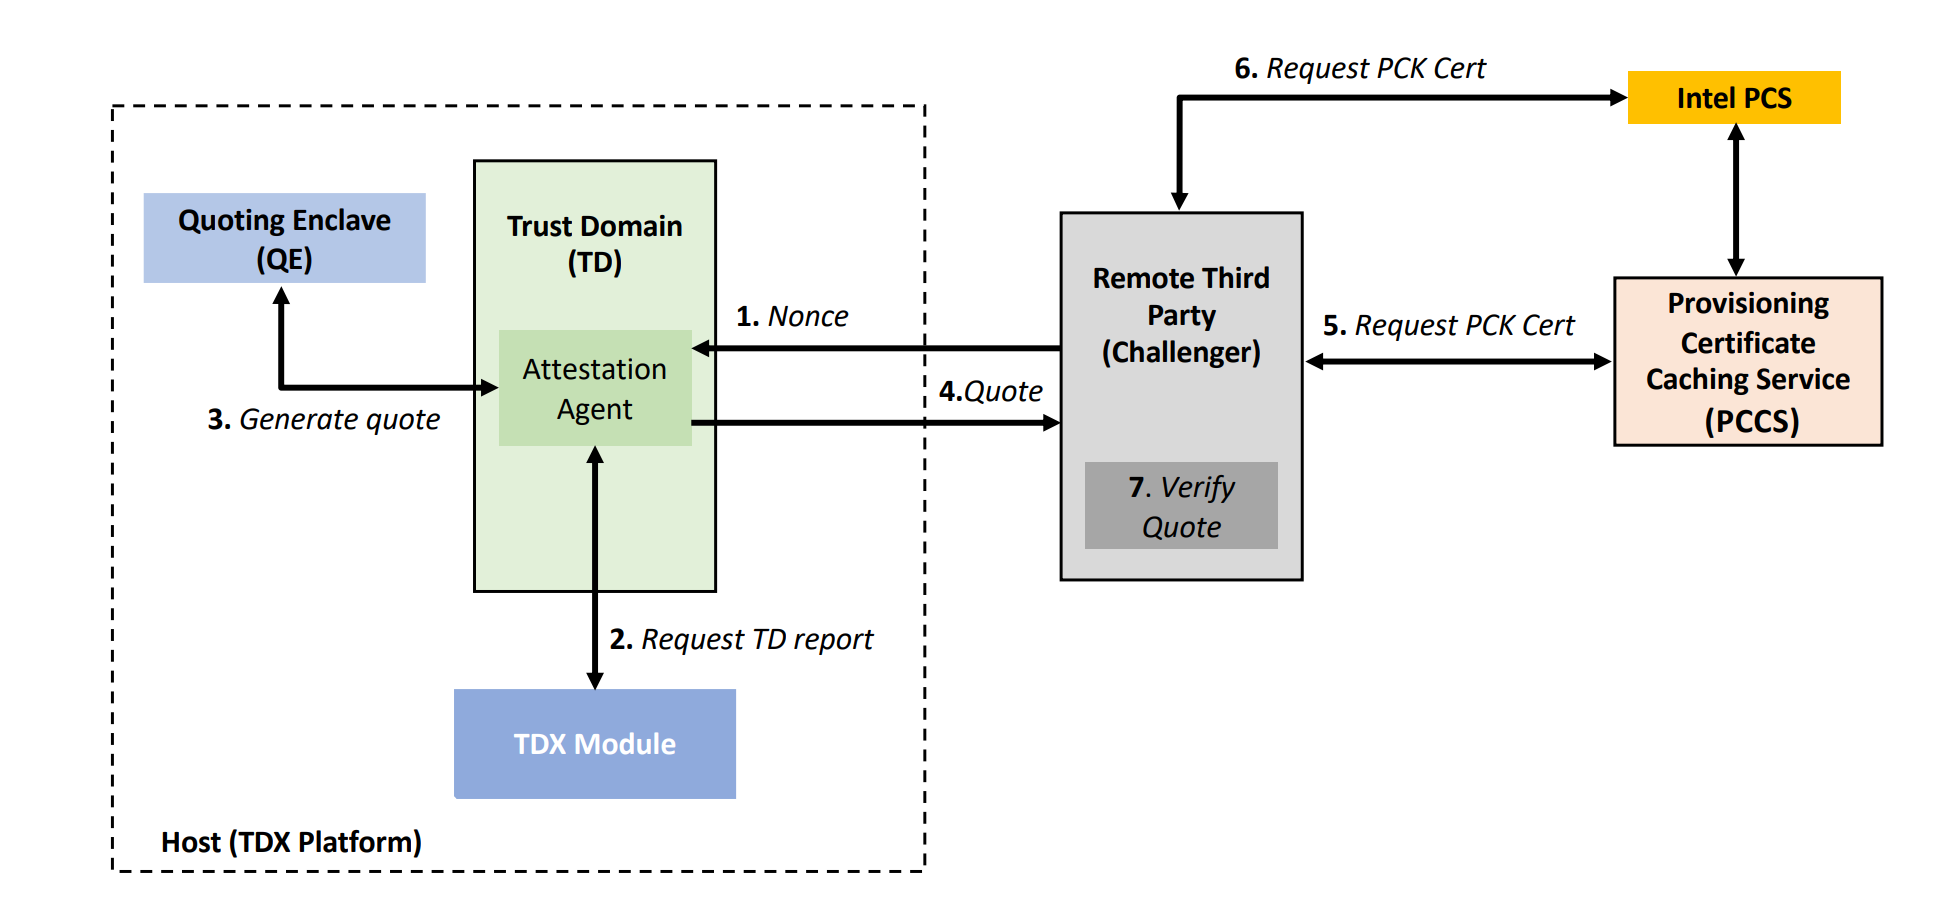
\includegraphics[width=\textwidth]{images/tdx_attestation_flow.png}
      \caption{Attestation workflow (from~\cite*{DBLP:journals/corr/abs-2303-15540})}
      \label{fig:tdx_attestation_flow}
  \end{subfigure}
  \hfill
  \begin{subfigure}[b]{0.3\textwidth}
      \centering
      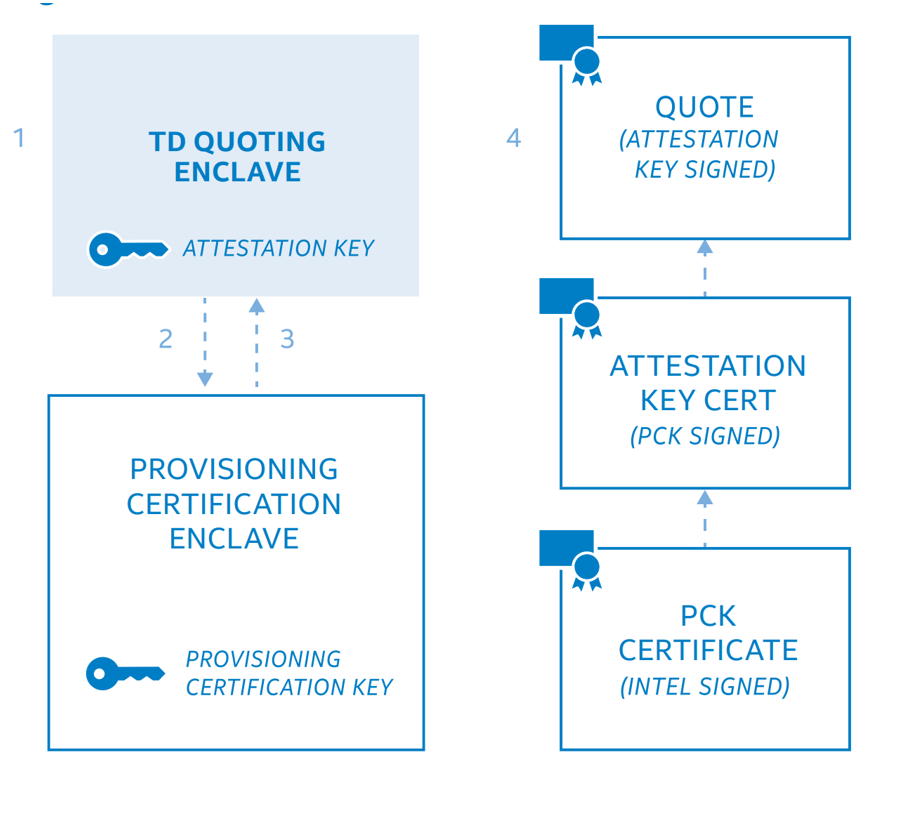
\includegraphics[width=\textwidth]{images/tdx_certi_chain.png}
      \caption{Certificate chain (from~\cite*{Intel_tdx_whitepaper})}
      \label{fig:tdx_certi_chain}
  \end{subfigure}
  \hfill
     \caption[Intel TDX remote attestation]{Intel TDX remote attestation}
     \label{fig:tdx_attestation}
\end{figure}

TDX leverages the Intel SGX attestation infrastructure for remote attestation~\cite*{Intel_tdx_whitepaper}, as shown in Figure~\ref{fig:tdx_attestation} (a).
The workflow begins with the TD requesting the TDX Module to generate a local report. This report includes the TD's measurements, TD-provided data, etc~\cite*{Intel_tdx_whitepaper}. The integrity of this report is protected by the CPU's HMAC key.
After generating the local report, the TD sends it to the quoting enclave,  which resides on the same platform. The quoting enclave first request the CPU to verify the report's MAC. Then, it utilizes its attestation key to generate a signature based on the 
report content. The report content and the signature form a quote. Notably, the attestation key of the quoting enclave is certified by the Platform Certification Enclave (PCE) using the Provisioning Certification Key (PCK), which is itself certified by Intel.
Consequently, the signature of the quote forms a chain of signatures, as illustrated in Figure~\ref{fig:tdx_attestation} (b). The certificate chain can be used to verify the authenticity of this report off the platform. Subsequently, the TD transmits the quote to the TD owner. 
The owner can verify the quote's signature by downloading the certificates from  
either the Platform Certificate Signing Service (PCCS) or intel Provisioning Certification Service (PCS)~\cite*{DBLP:journals/corr/abs-2303-15540}.
Finally, by examining the report's contents, the TD owner can determine whether the TD is genuine.  Note that a detailed explanation of the above workflow can be found in \cite*{DBLP:journals/corr/abs-2303-15540}. 

\subsection{Comparison of AMD SEV-SNP and Intel TDX}
Figure~\ref{fig:snp_tdx_compare} compares the features of Intel TDX and AMD SEV-SNP~\cite*{amd_sev_summarize}. In particular, the widely used \acrshort{TEE}, Intel SGX~\cite*{INTEL_SGX}, is chosen 
as a reference.

\begin{figure}[htp]
  \centering
  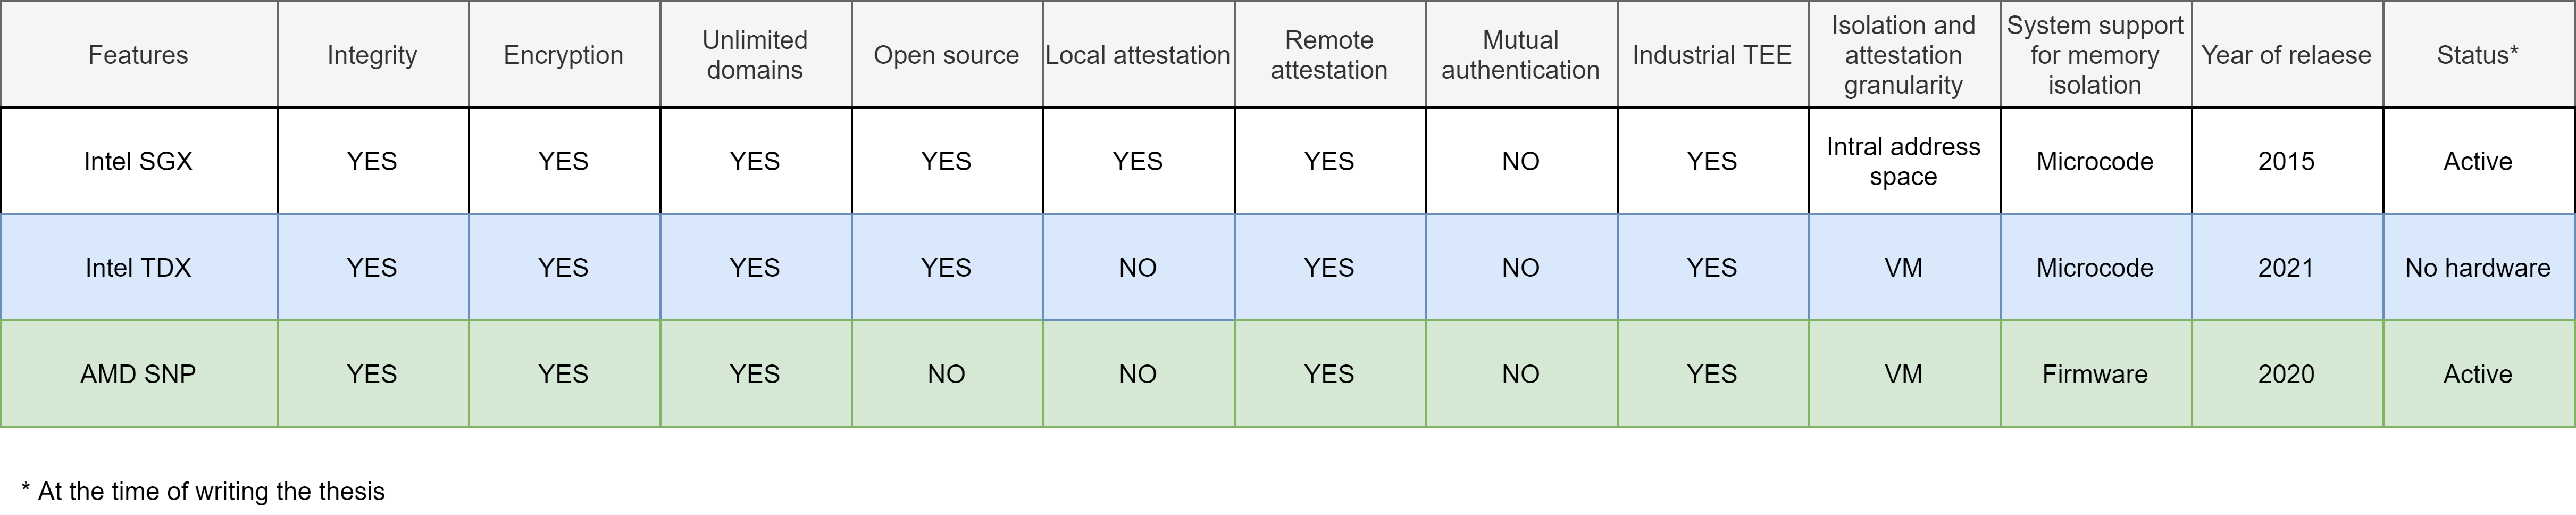
\includegraphics[width=1\textwidth]{images/snp_tdx_compare.png}
  \caption[Comparison of AMD SEV-SNP and Intel TDX]{Comparison of AMD SEV-SNP and Intel TDX~\cite*{amd_sev_summarize}}
  \label{fig:snp_tdx_compare}
\end{figure}




\section{KBS Attestation Protocol}
\label{sec:kbs}





The KBS attestation protocol~\cite*{kbs_Attestation_protocol}  presents a mechanism for remote attestation and provisioning. As shown in Figure~\ref{fig:kbs_overwiev}, this protocol involves the Key Broker Service (\acrshort{KBS}) and the Key Broker Client (\acrshort{KBC}). Typically, a \acrshort{KBC} refers to a confidential virtual machine or enclave that runs containers, while the 
\acrshort{KBS} acts as a secret manager. The KBS can utilize this protocol to attest a KBC and securely transmit secrets to it. Besides, the protocol employs TLS\cite*{tls_record_size} to prevent malicious attackers 
from hijacking the \acrshort{KBS} address,  impersonating the \acrshort{KBS},  and injecting harmful data into the \acrshort{KBC}~\cite*{kbs_Attestation_protocol}. Specifically, the protocol requires that the \acrshort{KBS}'s public key be effectively distributed to the \acrshort{KBC} so 
that the \acrshort{KBC} can authenticate the \acrshort{KBS} during the TLS handshake.
\begin{figure}[htp]
  \centering
  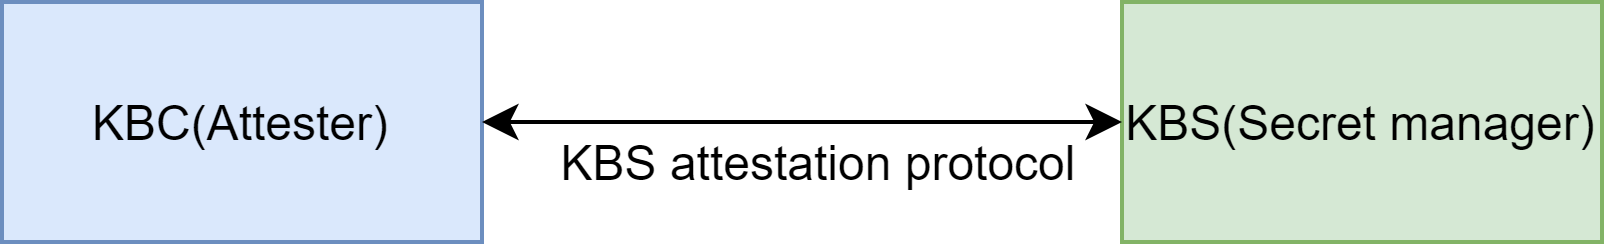
\includegraphics[width=0.6\textwidth]{images/kbs_overwiev.png}
  \caption[Overview of KBS attestation protocol]{Overview of KBS attestation protocol}
  \label{fig:kbs_overwiev}
\end{figure}


The protocol is divided into two phases. The first phase is the authentication phase, where the \acrshort{KBS} authenticates the \acrshort{KBC} using the \acrshort{KBC}'s attestation report. The second phase is the resource request phase, in which the \acrshort{KBS} allows the \acrshort{KBC} to retrieve a secret managed using the HTTP GET.  
The secret transmitted from the \acrshort{KBS} to the \acrshort{KBC} is encrypted using the \acrshort{KBC}'s public key. The public key is sent to the \acrshort{KBS} with the \acrshort{KBC}'s attestation report during the first phase. Because the hash of the public key is included in the \acrshort{KBC}'s attestation report, the \acrshort{KBS} can confirm that the public key is from the \acrshort{KBC} and ensure that only the \acrshort{KBC} can decrypt the encrypted secret. Additionally, the \acrshort{KBS} assigns an HTTP cookie to the \acrshort{KBC} during the authentication phase. This cookie associates the authentication result obtained in the first phase with the corresponding \acrshort{KBC}. During the resource 
request phase, \acrshort{KBS} uses this cookie to find the \acrshort{KBC}'s authentication result and considers it along with the secret owner defined policy to determine if a secret should be provided to the \acrshort{KBC}. The following two diagrams detail how \acrshort{KBS} and \acrshort{KBC} work in phases 1 and 2:


\begin{figure}[htp]
    \centering
    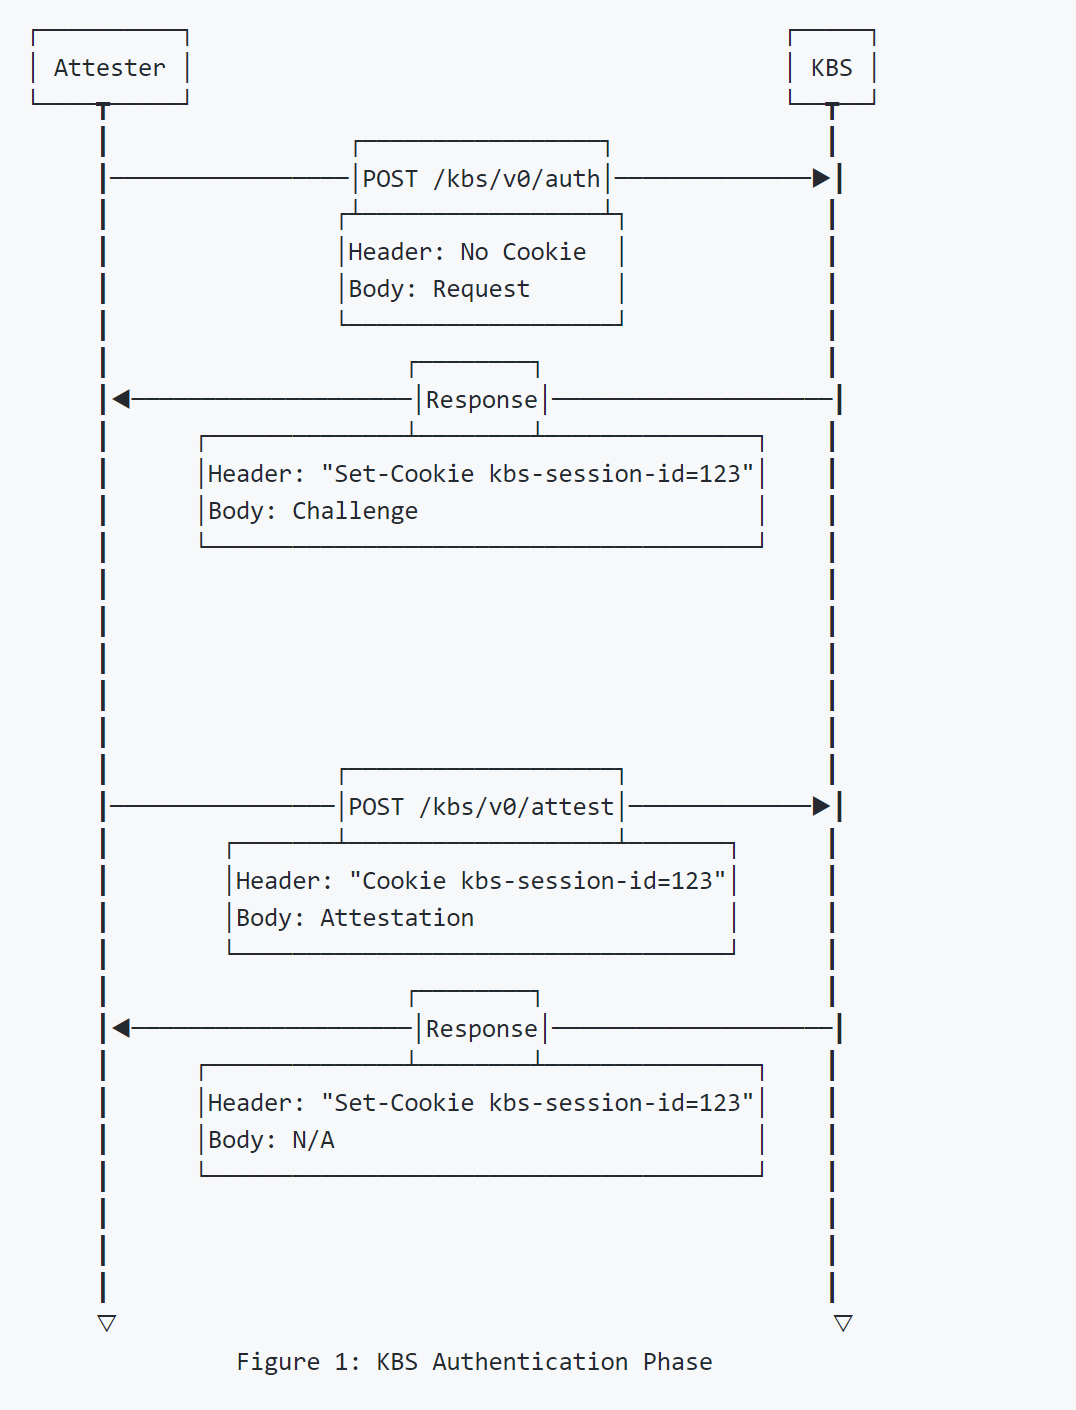
\includegraphics[width=0.5\textwidth]{images/attestation.PNG}
    \caption[Authentication phase]{Authentication phase from~\cite*{kbs_Attestation_protocol}}
    \label{fig:Authentication}
\end{figure}

As defined in the key broke service attestation protocol, phase 1 (authentication phase) has four steps: 
\begin{displayquote}
    \begin{enumerate}
        \item  \texttt{Post /kbs/v0/auth}: The KBC sends an HTTP Post whose body is a KBS Request JSON payload to KBS to initiate the attestation protocol. The payload contains The protocol version number supported by KBC, the type of HW-TEE platform where KBC is located.
        \item  Response: The KBS responds with the Challenge payload, which contains an attestation challenge (nonce) for the attester. In the next step, KBC must place it in the evidence sent to the KBS to prevent replay attacks. Furthermore, the KBS also sends a session identifier to the KBC as an HTTP Cookie
        \item  \texttt{Post /kbs/v0/auth}: The KBC sends an HTTP Post request with a JSON payload called KBS Attestation and a cookie set to the value received in the previous step. The payload contains the attestation evidence and the KBC’s public key.
        \item  Response: Upon successful attestation, the KBS replies to that request with an empty payload and sets the status code to 200. KBC can check the status code to determine if the authentication succeeds. 
    \end{enumerate}
\end{displayquote}

\begin{figure}[htp]
    \centering
    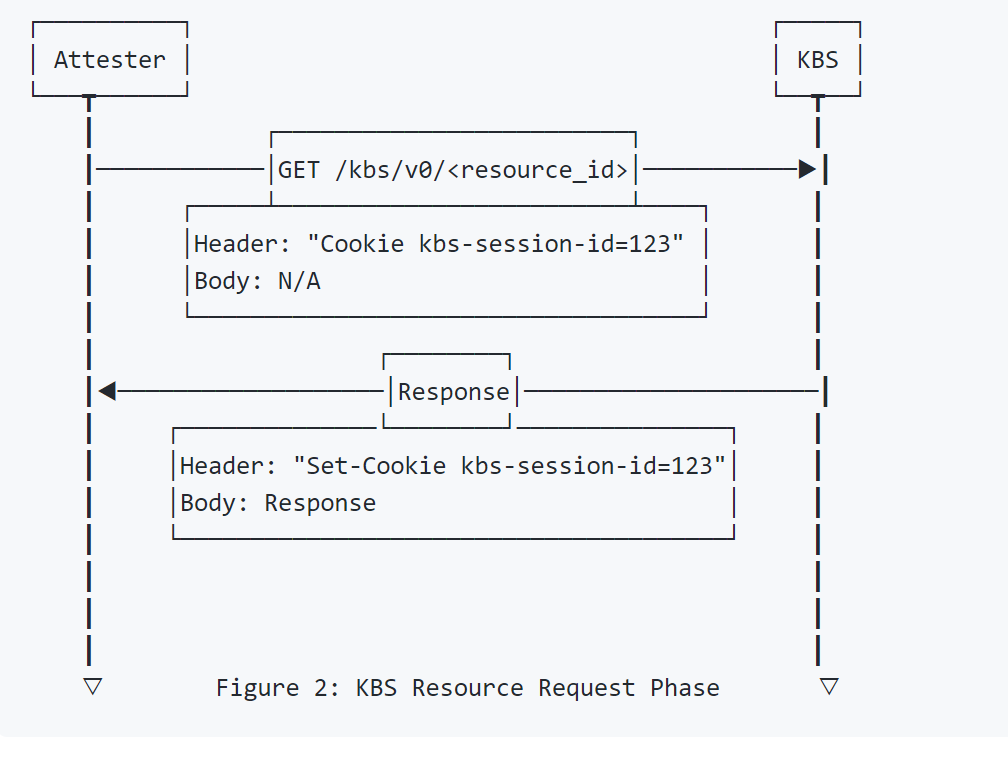
\includegraphics[width=0.5\textwidth]{images/resourcerequrie.PNG}
    \caption[Resource Requests phase]{Resource Requests phase from~\cite*{kbs_Attestation_protocol}}
    \label{fig:resourcerequrie}
\end{figure}
As defined in the key broke service attestation protocol, \acrshort{KBC} can request resources or services from KBS during the second phase in the following way:
\begin{displayquote}
  To request a protected resource from the KBS, the attester sends a GET request to a resource-specific endpoint. If the attester can access the resource, the KBS will respond to the GET request with an HTTP response in which content is set to a KBS Response JSON payload.
\end{displayquote}


\section{Summary}
This chapter first introduced Kubernetes~\cite*{k8s} and the concept of high and low-level container runtimes. Subsequently, the standards and interfaces that enhance the scalability of Kubernetes were explained, specifically CRI~\cite*{cri-interface}, OCI~\cite*{oci-runtime-spec}, and 
\texttt{shim v2 API}~\cite*{shim_v2}.
Then, the architecture of the Kata and Quark container~\cite*{Kata-Containers, quark} was explained. Furthermore, TEE-related concepts such as memory protection and remote attestation were illustrated using AMD SEV-SNP~\cite*{SEV_SNP_white_book} and Intel TDX~\cite*{Intel_tdx_whitepaper} as 
examples. Lastly, a brief description of the KBS attestation protocol~\cite*{kbs_Attestation_protocol} was provided.
\cleardoublepage


\chapter{Security Analyze}
\label{sec:security_analyse}

% Ist das zentrale Kapitel der Arbeit. Hier werden das Ziel sowie die
% eigenen Ideen, Wertungen, Entwurfsentscheidungen vorgebracht. Es kann
% sich lohnen, verschiedene Möglichkeiten durchzuspielen und dann
% explizit zu begründen, warum man sich für eine bestimmte entschieden
% hat. Dieses Kapitel sollte - zumindest in Stichworten - schon bei den
% ersten Festlegungen eines Entwurfs skizziert werden.
% Es wird sich aber in einer normal verlaufenden
% Arbeit dauernd etwas daran ändern. Das Kapitel darf nicht zu
% detailliert werden, sonst langweilt sich der Leser. Es ist sehr
% wichtig, das richtige Abstraktionsniveau zu finden. Beim Verfassen
% sollte man auf die Wiederverwendbarkeit des Textes achten.

% Plant man eine Veröffentlichung aus der Arbeit zu machen, können von
% diesem Kapitel Teile genommen werden. Das Kapitel wird in der Regel
% wohl mindestens 8 Seiten haben, mehr als 20 können ein Hinweis darauf
% sein, daß das Abstraktionsniveau verfehlt wurde.

%\ldots design \ldots

%\todo{write design}

This chapter aims to analyze the potential vulnerabilities in Vanilla Quark, through which an adversary can obtain access to confidential information of an application. The first section defines the threat model(Section~\ref{sec:Threat_model}). 
Subsequently, this chapter scrutinizes the Vanilla Quark's security from the perspective of the Open Container Initiative (OCI) interface (Section~\ref{sec:security_analysis}).



\section{Threat model}
\label{sec:Threat_model}
We employs the OWASP application threat modeling methodology\cite*{OWASP_Threat_Modeling} to create a threat model comprising four aspects: Actors, assets , external dependencies, and attack surface.

\textbf{Actors}. Our model involves the cloud provider and the tenant. While the cloud provider is accountable for providing the hardware and software necessary for running and orchestrating applications, the tenant distrusts the cloud provider 
in the context of a confidential computing environment. Therefore, any software components within the cloud infrastructure - Kubernetes control plane\cite*{k8s}, containerd\cite*{containerd}, and hypervisor are untrusted.

\textbf{Assets}. Our objective is to secure the Kubernetes workload(application) itself, i.e., preserving the integrity of the application binary and its dependencies, maintaining the confidentiality and integrity of the data generated by the 
application during runtime, as well as protecting the secrets provided to the application by its owner.

\textbf{External Dependencies}. We assume that the Guests, including Qkernel and Kubernetes workloads, operate within an encrypted virtual machine to prevent malicious hypervisor(Qvisor) or powerful cloud operator from accessing the workload’s 
sensitive data through guest memory and registers. Furthermore, we exclude attacks related to denial of service\cite*{DOS_ATTACK}, side channell\cite*{217454}, 
network, or file systems.

\textbf{Attack Surface}. We primarily focus on attacks occurring on the OCI interface\cite*{oci-runtime-spec}. As the management of k8s workloads is the responsibility of the cloud provider, it must have a means of accessing workloads for 
orchestration, even if the workloads are running within a TEE. Although the OCI runtime specification offers this possibility to the cloud provider, it exposes a new attack surface for an adversary to probe k8s workloads’ secrets. Additionally, 
since the implementation of OCI in the guest interacts with the host through the Hypercall, Qcall, or Ucall interface, we also considered attacks from this interface.

\section{Security Analysis}
\label{sec:security_analysis}

This section provides an in-depth security analysis of the implementation of the OCI runtime interface within Quark.  Notably, Qlib serves solely as a development concept since Qlib code is incorporated into the Qkernel and Qvisor binaries during 
the compilation. Therefore, the following sections use Qkernel and Qvisor to refer to the respective binaries containing the qlib code.

The subsequent subsections thoroughly examine the potential pitfalls of the OCI implementation in Quark in the context of confidential computing from seven perspectives. These include application secrets deployment, handling  STDIO of guest user 
space process, command execution and terminal allocation, paravirtualized file system sharing, guest system call,  guest kernel arguments, and guest logging system. The Design chapter further proposes mechanisms to mitigate these vulnerabilities.

\subsection{Application Secrets Deployment}
\begin{figure}[H]
    \centering
    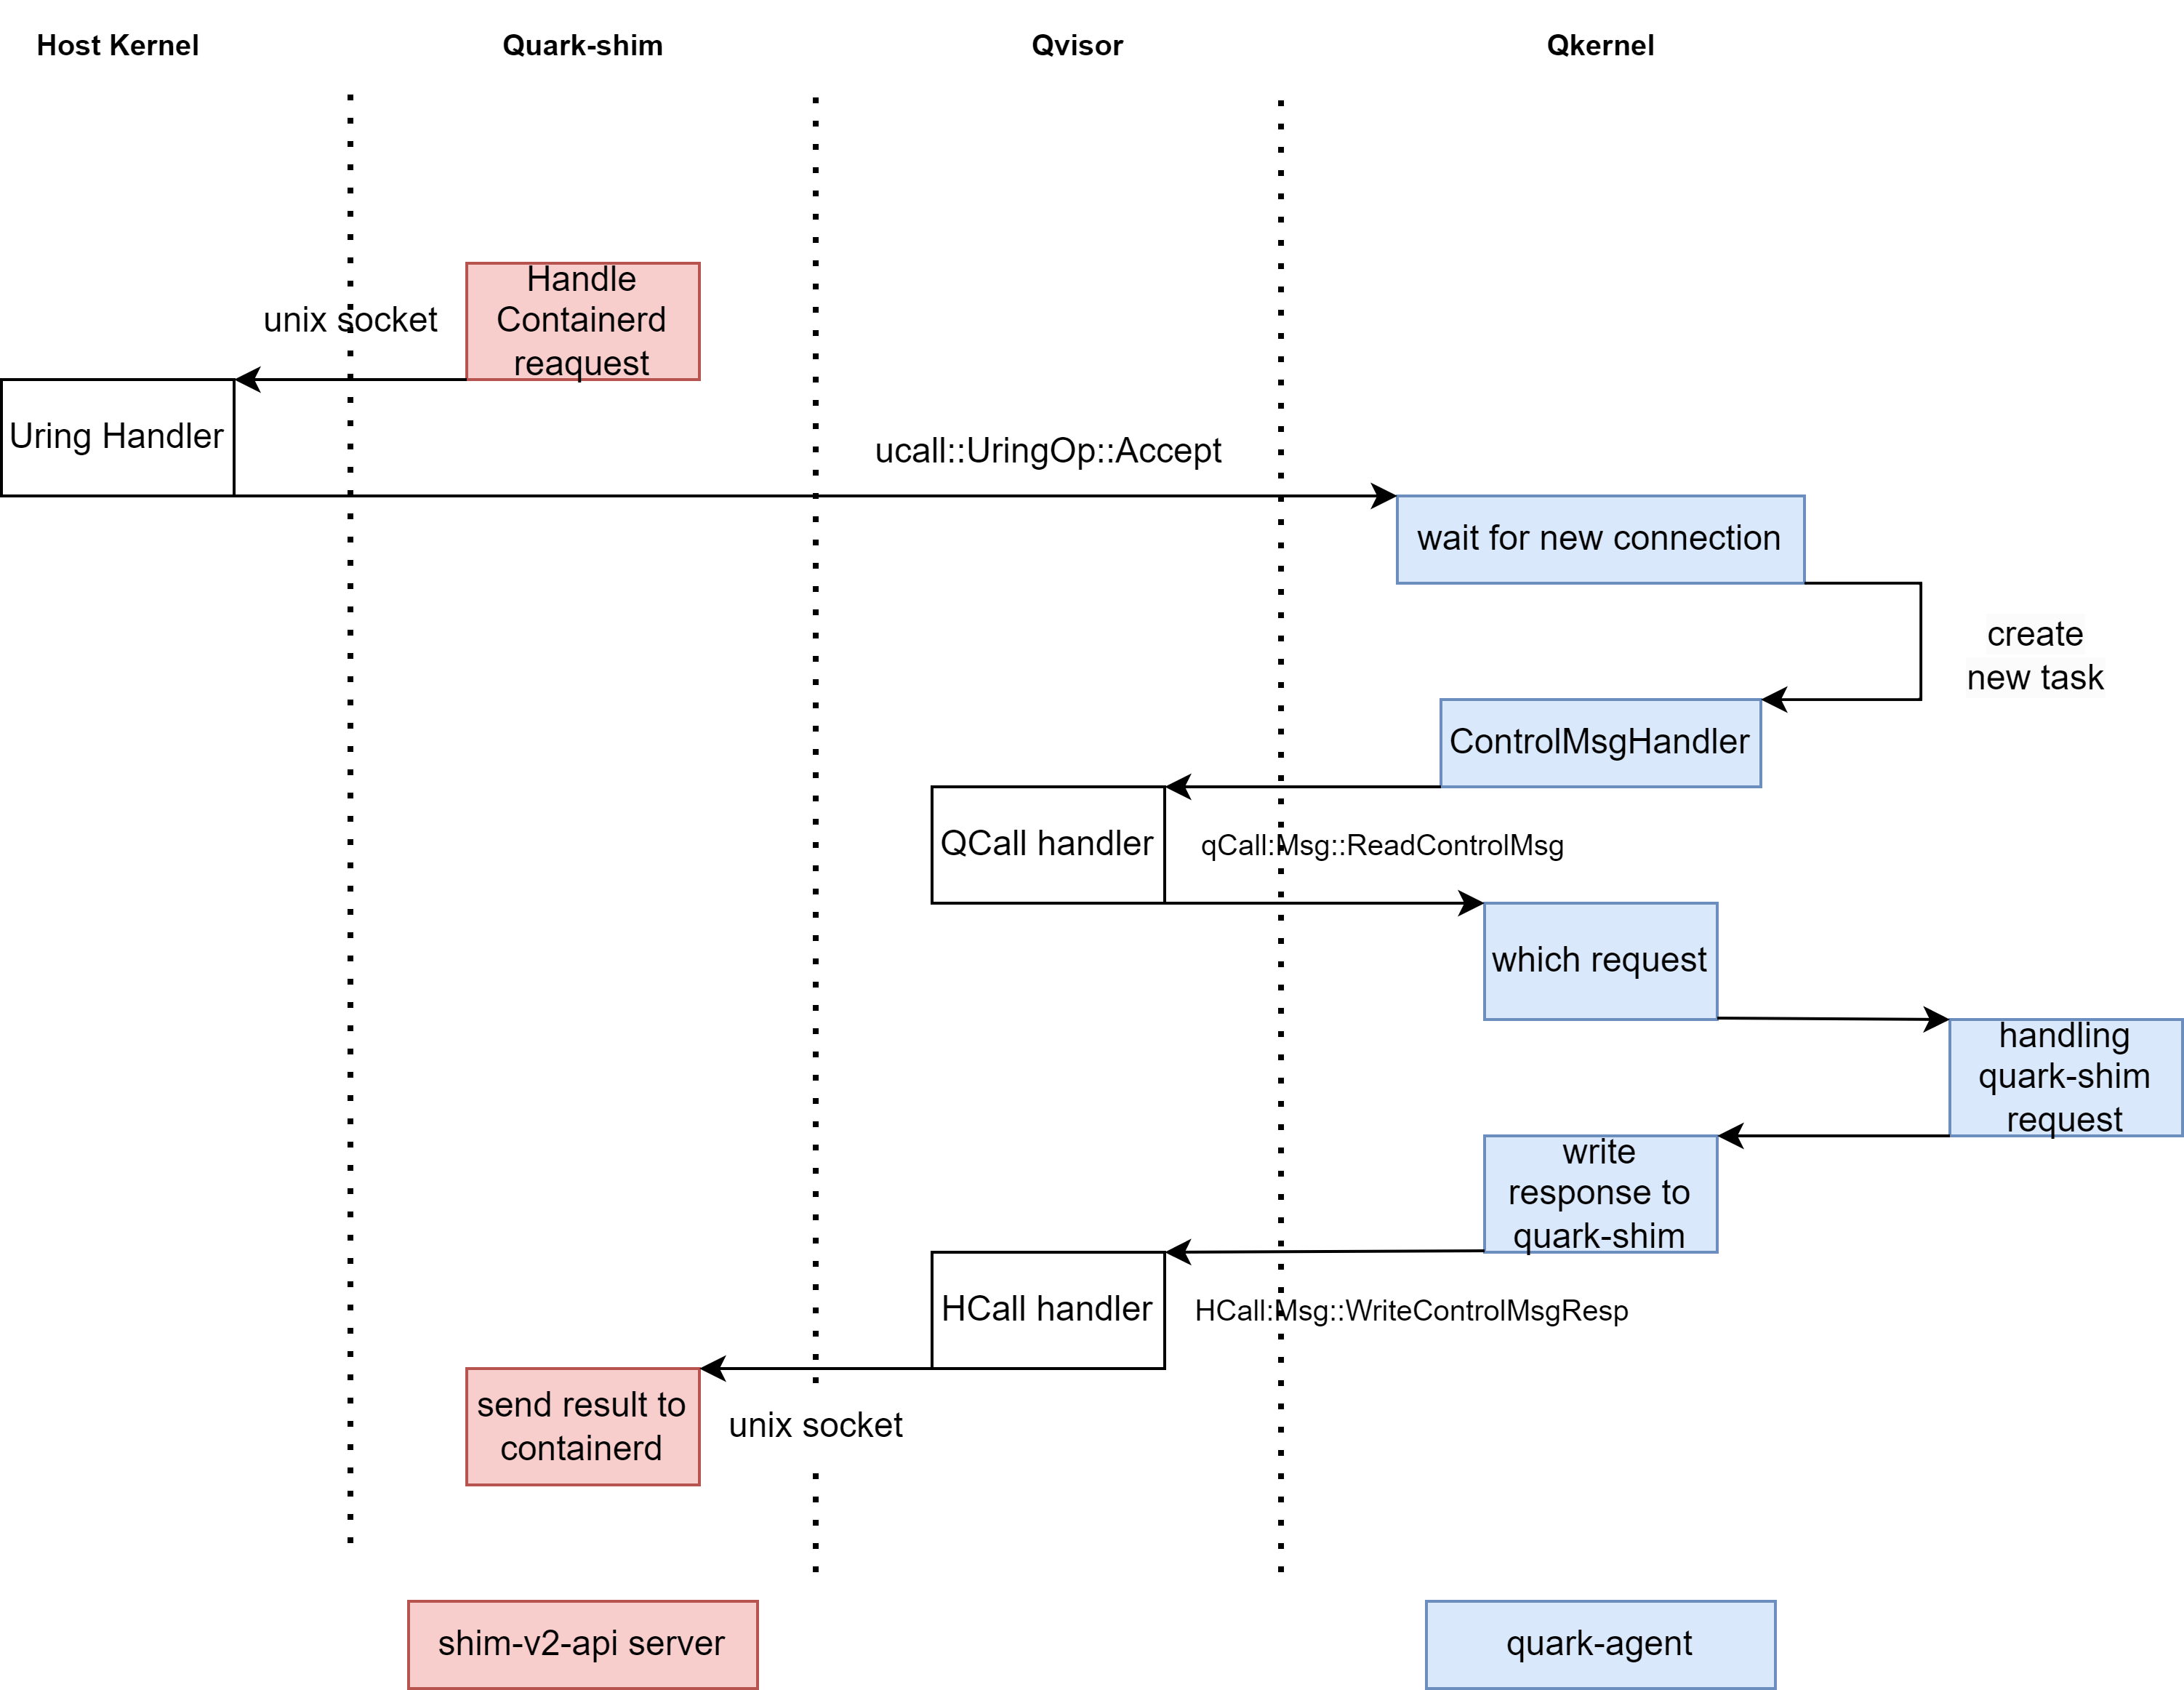
\includegraphics[width=0.8\textwidth]{images/quark-agent-work-flow.png}
    \caption[Quark Agent Workflow]{Quark Agent Workflow. The Quark agent is located in the qkernel. It is responsible for receiving requests from quark-shim, like creating application processes, creating exec processes, deleting a
    pplication processes, etc.}
    \label{fig:quark_agent_work_flow}
\end{figure}


\textbf{Application secrets are managed and deployed by untrusted Kubernetes and the Quark shim process}. These secrets may be injected into the application through command line arguments, mounted files, or environment variables. When deploying 
the application, Containerd generates an Application Bundle and transmits it via the shim v2 API\cite*{shim_v2} to the shim-v2-api server in the quark-shim process. This bundle contains the rootfs of the application along with an OCI-compatible config.json file. Quark-shim 
creates the root filesystem for the container on the host-side, mounts the file type secret, establishes the process spec with the command line type, the environment variable type secrets, and uses the Unix socket to request the Quark 
Agent in the Qkernel to create an application process based on this process specification. The workflow is shown in figure~\ref{fig:quark_agent_work_flow}.


Quark-agent operates as a socket server accepting connection requests from the Quark shim through Ucall::Uringop::accept(). These requests include creating and deleting application processes and creating an exec process 
and etc. Upon receiving a request from the quark-shim to create an application (exec) process, the Uringop::accept returns a host file descriptor that contains the process specification sent by the quark-shim. As the quark agent in the qkernel cannot
 read its contents directly, it employs qcall: Msg::ReadControlMsg to request the Qvivor to read the file descriptor and return the process specification. The process specification provides metadata for creating a process, including command line arguments, environment variables, the type of STDIO (terminal or normal IO), and the host file descriptor that is used for transmitting data from/to the process STDIO. Based on this process specification, Quark-agent creates a guest user process. Specifically, the command line arguments and the environment variables are pushed to the process stack, and the STDIO of the process is set accordingly to the type of STDIOspecified in the specification. Further details about the process's STDIO can be found in section XX.

Given the untrustworthiness of the Kubernetes control plane\cite*{k8s}, Containerd\cite*{containerd}, Quark shim, and Qvisor, employing Kubernetes to manage application secrets (file type, command line type, environment variable type secrets) and deploying them through 
Containerd and Quark shim is imprudent. In particular, individuals with access to the cluster can use the kubectl describe pod-name command to view the application's environment variables and command-line arguments, or the kubectl edit secrets 
or kubectl get secret commands to access and modify file secrets. Additionally, it is possible for an adversary to manipulate Containerd and Quark shim during application deployment to tamper with the application secrets by modifying the application 
bundle. Last but not least, when Quark-agent uses the Qcall interface to request Qvisor to read the process specification containing secrets, Qvisor could potentially steal or modify these secrets. To mitigate these security risks, we suggest 
offloading secret deployment and management from k8s, Quark-shim, and Qvisor. For a detailed explanation of the mitigation, please refer to section XX.

\subsection{Guest User Space Process STDIO}
The Quark-agent loads the corresponding binary and initiates a guest user space process for handling the request of either creating an application or executing a command (kubectl exec)\cite*{k8s}. Thus, Quark handles the application process STDIO 
in the same way as it handles the exec process STDIO. For instance, when Containerd wishes to create an exec process in Qkernel, three named pipes are created for the process’s standard input, output, and error. These are then passed to Quark-shim 
via the quark-shim-v2 API along with other metadata, from which Quark-shim creates the exec request's process specification. The Quark handles STDIO of the process differently based on the terminal keyword in the process specification. 

\begin{figure}[ht] 
    \begin{subfigure}[b]{0.5\linewidth}
      \centering
      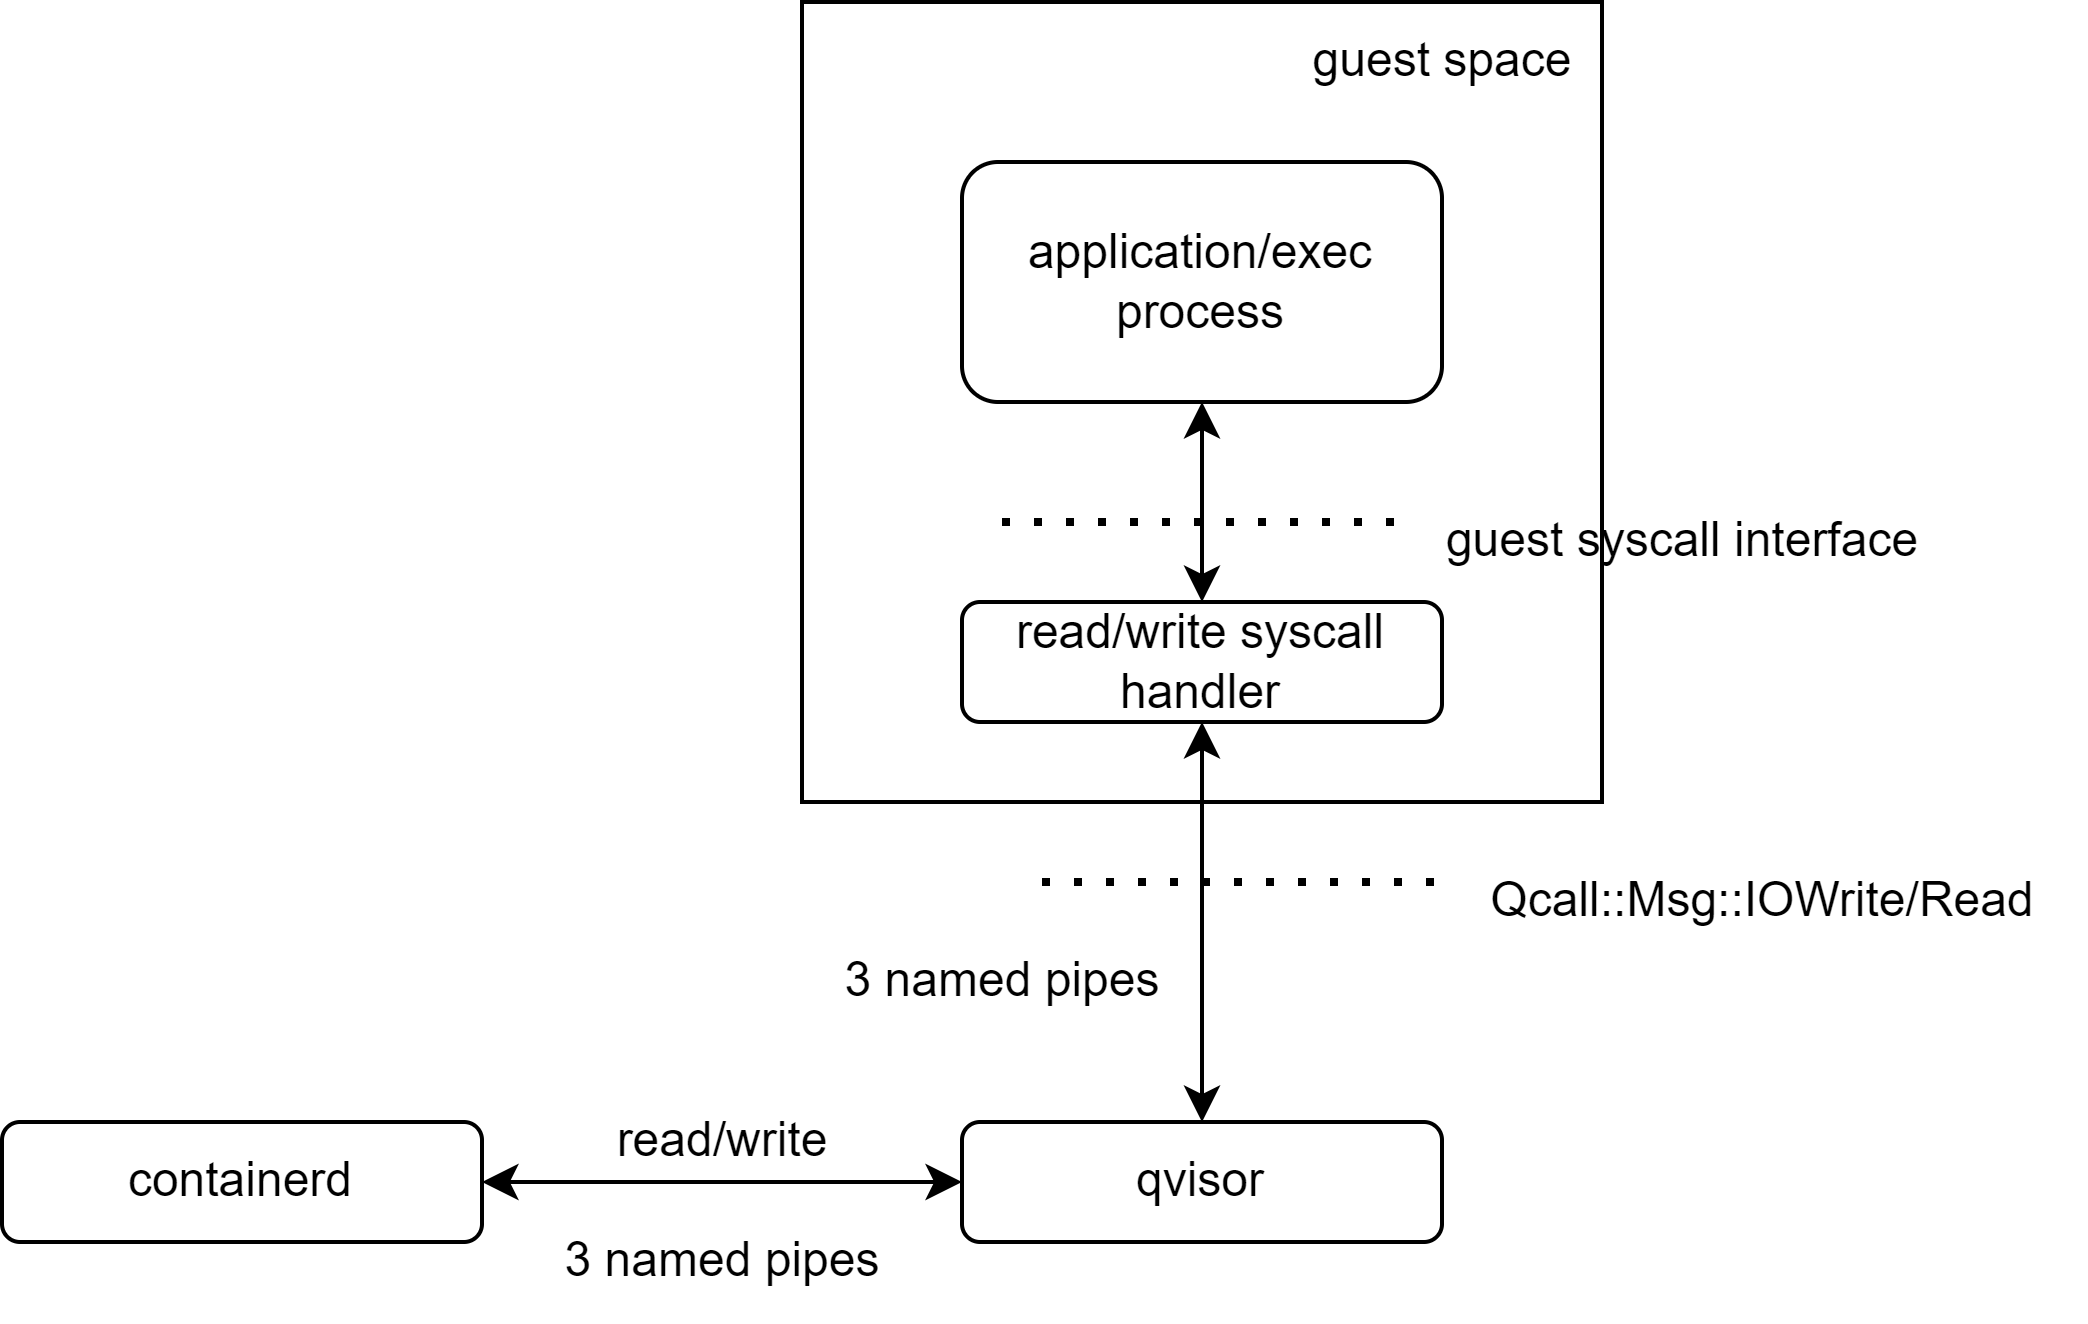
\includegraphics[width=0.9\linewidth]{images/normorl_io.png} 
      \caption{Normal IO} 
      \label{fig1:a} 
      \vspace{4ex}
    \end{subfigure}%% 
    \begin{subfigure}[b]{0.5\linewidth}
      \centering
      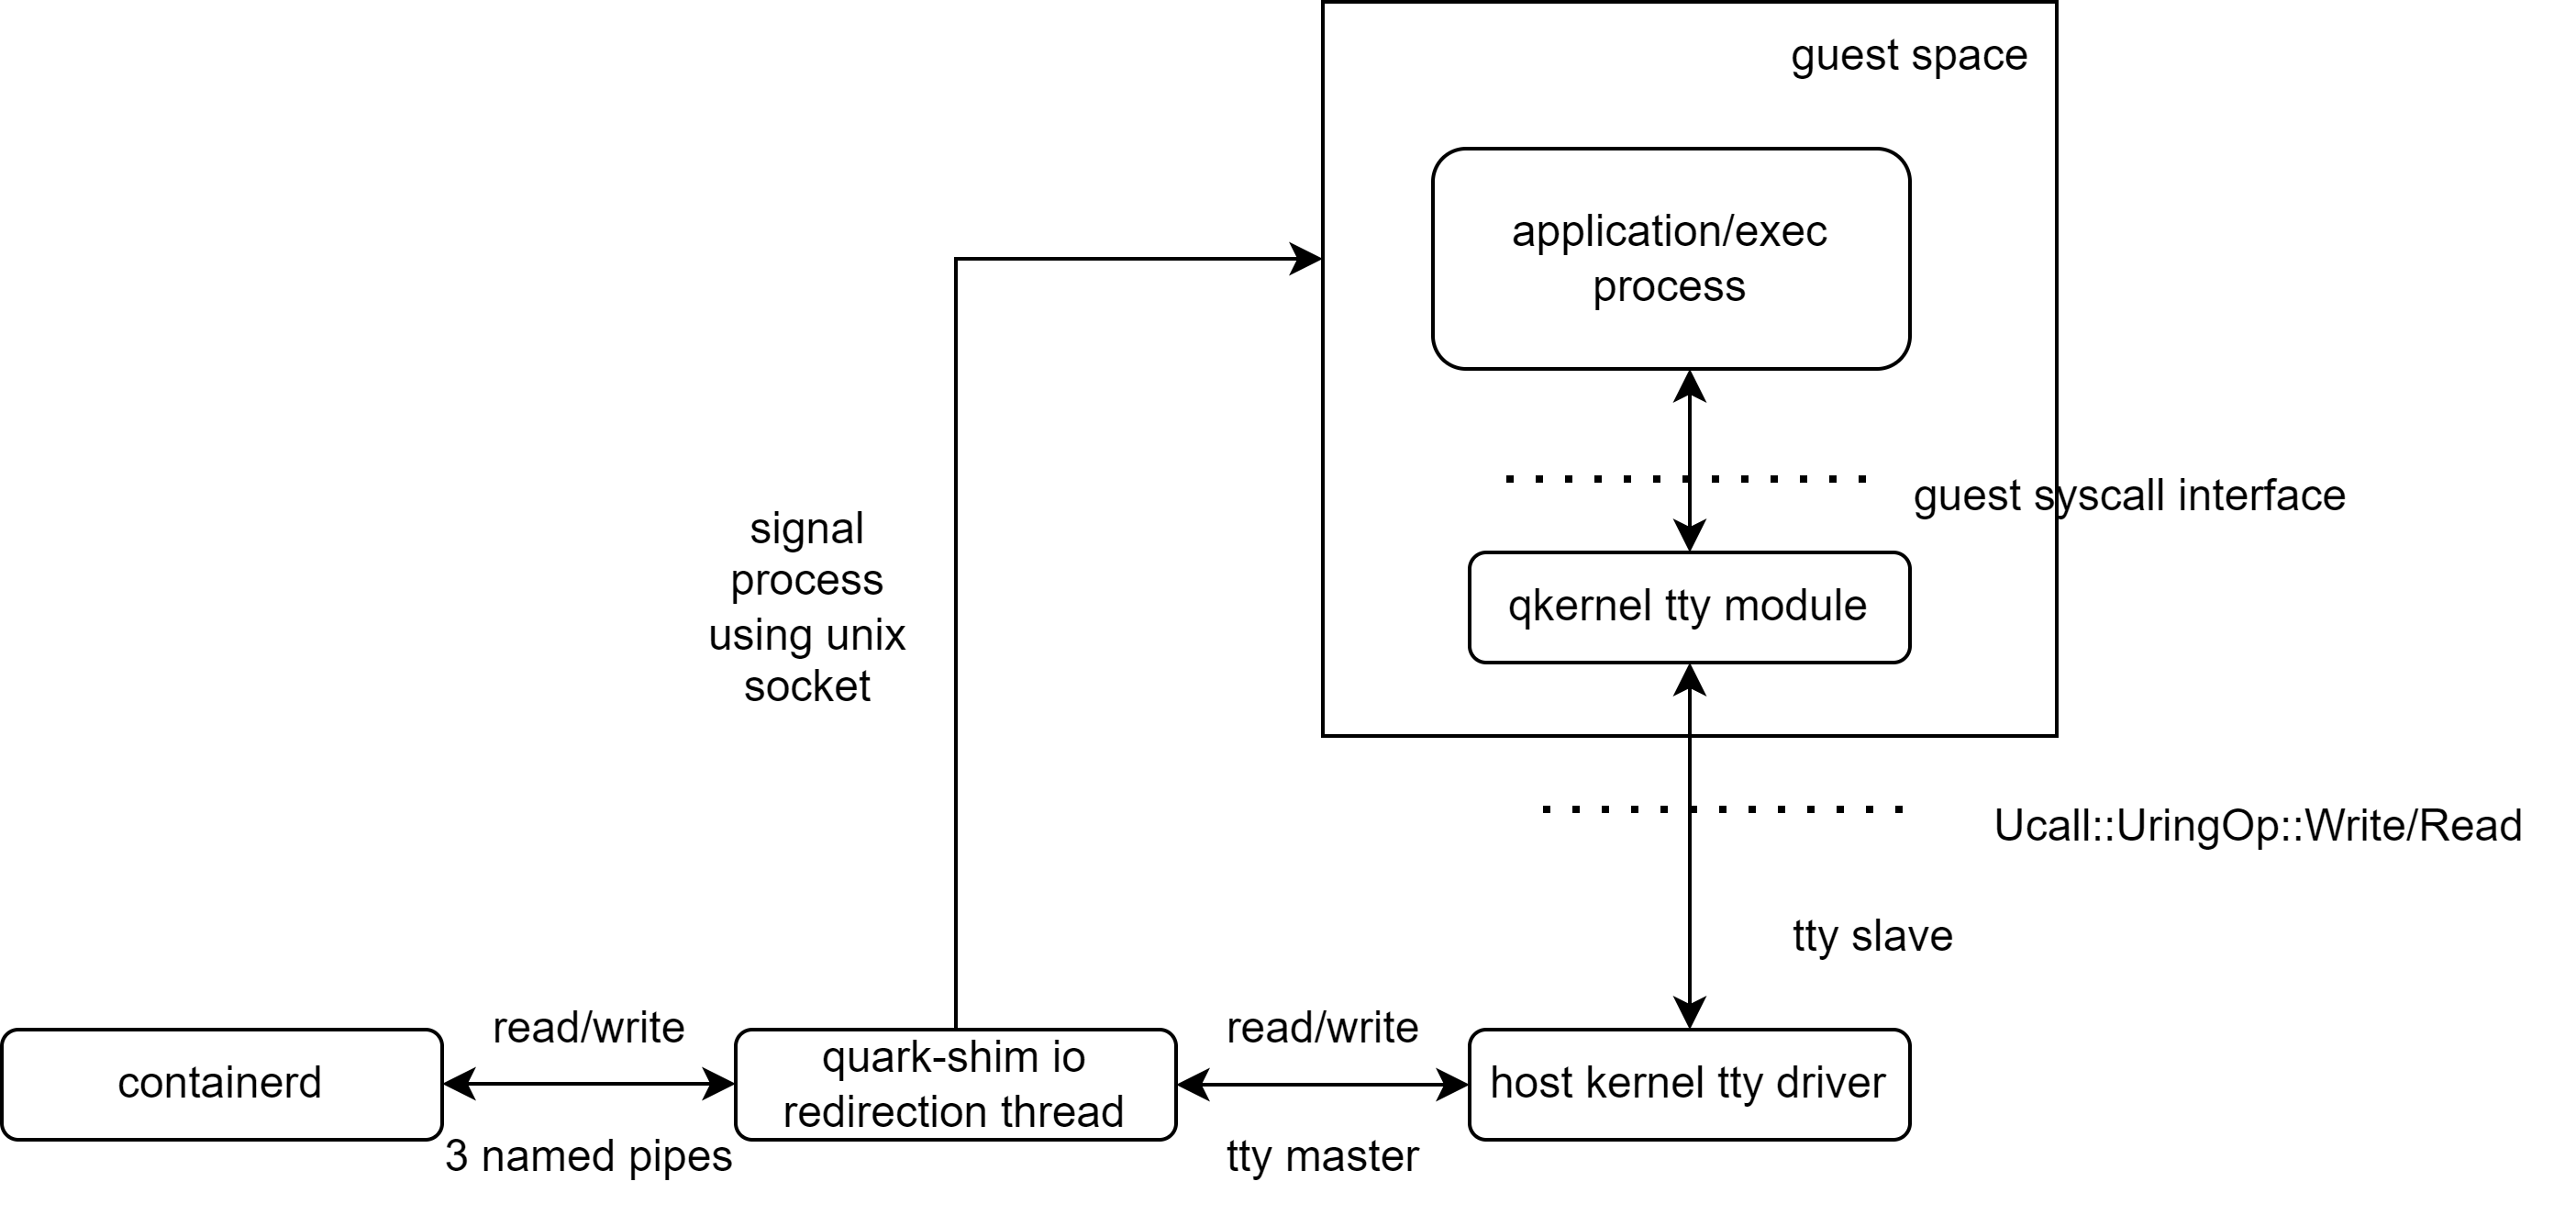
\includegraphics[width=0.9\linewidth]{images/termianl_workflow.png} 
      \caption{Terminal IO} 
      \label{fig1:b} 
      \vspace{4ex}
    \end{subfigure} 
    \caption{Guest User Space Process STDIO Handling Workflow}
    \label{fig1} 
\end{figure}


When the terminal keyword is set to true, Quark-shim creates a terminal IO redirection thread and a TTY pair (TTY master and TTY slave) in raw mode. The file descriptor of the TTY slave is then sent to the Quark-agent, where it is set as stdin, 
stdout, and stderr of the process. The terminal IO thread in Quark-shim (as illustrated in Figure~\ref{fig1:b} ) filters the signals in the STDIN-named pipe and transfers the data between tty master and the named pipes. The filtered signals include SIGINT, 
SIGQUIT, and SIGTSTP, which are forwarded to Quark agent via the unix socket and passed to the corresponding processes. For instance, when the character \verb|^C| (ASCII code 3) appears in the STDIN-named pipe, the terminal IO thread sends SIGINT to 
the exec process, ultimately terminating the process. Furthermore, the Qkernel manages the tty slave by implementing a tty module. This module reads and writes the TTY slave through the UCLL interface. The data written to tty master and 
slave are processed by the host kernel TTY driver, which is responsible for character echoing, automatic conversion between carriage returns and linefeeds, editing the qkernel returned data (adding /r before /n, then adding "/ \#"), and 
notifying that process the data exist in its stdin by unblocking the process. Note that the terminal works only when the guest user process's stdin is interactive, i.e., the stdin must be a tty slave, thus, without this driver, the terminal won’t work. Conversely, when the terminal keyword is set to false, 
Quark-shim directly send the three named pipes to the Quark agent, which then creates the exec process and uses the three named pipes as standard input, out and error. Unlike the former case, Qkernel uses the Qcall interface for STDIO data 
transmission if a file descriptor is of the pipe type (Figure ~\ref{fig1:a}). While the process is running, Containerd will keep the three named pipes representing the process STDIO open. For the application process, both stdout and stderr stream 
output are saved as log information to a location specified by Kubernetes. For the exec process, command execution results are returned to the user either via stdout or stderr.


\textbf{Absence of end-to-end encryption for terminal data streams}. When the terminal keyword is true in a process specification, the STDIO of exec or application processes is of the terminal type. This poses a serious threat to the confidentiality and 
integrity of the application data because of the manner in which untrustworthy Quark-shim process Terminal IO. In the field of computer security, man-in-the-middle attack\cite*{Man_in_the_middle_attack} is a common mode of attack where an attacker can intercept and forward 
messages between two parties with the purpose of eavesdropping or altering communications. In the case of Quark, the attacker can use Quark-shim as a man-in-the-middle to intercept confidential application data while the terminal redirection 
thread forwards the data. In severe cases, the attacker can change the commands sent by the application owner or tamper with the command results to achieve their ulterior motives.


\textbf{Lack of cryptographic protection for application log}. The standard output and standard error stream data generated by applications are managed uniformly as application logs by the kubenetes. However, this approach is inappropriate since our 
threat model does not trust the cloud infrastructure provider. An individual with cluster access can use the "kubectl logs pod-name" command to view the application logs, and a malicious administrator can log into the host running the application 
and view the application logs stored in the host file system. As a countermeasure, Qkernel should encrypt the application stdout and stderr stream data. Specific mitigation measures can be found in Section XX.

\textbf{Lack of cryptographic protection of exec request results}. When the application owner issues commands to the application, the returned execution results are often confidential and sensitive. However, these results are returned by untrusted entities 
such as qvisor and containerd (as shown in Figure 3). For instance, if the application owner issues the command "cat /var/log/confidential.log" to the application, the Quark-agent would create a process to execute the "cat" binary and write the 
result to the process's stdout. Notably, the process’s STDIO in this case is set to named pipes. Subsequently, the qkernel's write syscall handler requests the Qvisor through Qcall to write the result to the named pipe, from where the Containerd 
gets the result and sends it back to the user. This setup gibe both Qvisor and Containerd the ability to temper with the command's results. As such, it is crucial to cryptographically protect the stdout and stderr of processes that execute commands 
from application owner. Further details on the mitigation measures can be found in Sections XX.


\subsection{Issuing command and Terminal Allocation}
\textbf{Anyone can issue commands to an application}. Currently, the Quark agent (see section xx for an explanation) in the qkernel lacks authentication and access control on the exec requests sent from the quark shim.  Therefore,  allowing any 
user with access to the cluster to collect sensitive data of an application running inside a TEE by issuing commands to the application using kubectl exec.  An example of such access can be illustrated by executing kubectl exec pod-name printenv 
to obtain the application’s environment variable type secret. In response to this vulnerability, we have classified the exec commands into two separate categories as follows: “privileged” commands issued by the application owner, and “unprivileged” 
commands issued by other users. With regards to executing these commands, the Quark agent operates in accordance with the last privilege principle to authenticate and access control on the exec requests. Therefore, unauthorized requests will be 
denied. For further details, please refer to section X.

\textbf{The commands issued by privileged users may contain confidential data but are unprotected during transmission}. Currently, user-issued commands are sent to Quark-shim by conatinerd  as part of the exec request’s metadata via the shim-v2 API\cite*{shim_v2}. Quark-shim processes the exec request in 
a way similar to that used to create an application process. When Quark-shim receives an exec request, it generates a process specification based on the metadata, which includes the command to be executed and other relevant data such as 
terminal information. Quark-shim forwards this specification to the Quark agent via a Unix socket. The Quark agent then creates a guest userspace process to execute the command (see Figure 1). However, As Quark-shim and Containerd are 
untrusted, there is a potential for the commands to be compromised or modified during transit. To address this vulnerability, we should apply end-to-end cryptographic protection for privileged-level commands. The encryption occurs at the user end 
and decryption at the qkernel-side, preventing commands from being accessed by any untrusted parties during transmission. For additional information, see section XX.


\textbf{Any user can allocate a terminal In Kubernetes using one of two methods supported}: creating a terminal process within a pod by using kubectl exec -it pod-name, or setting stdin: true and tty: true in the container specification during 
application deployment and then attaching to the application process’s stdio using kubectl attach -it pod-name. It should be noted that the latter method only works if the application process is executing binaries like bash, sh, etc. that can 
receive commands from stdin.For Quark-shim and Quark-agent, this means that the keyword terminal is set to true in the process specification used to create the exex or application process. In this scenario, Quark agent then treats the process 
stdio as terminal, as explained in section XX. However, the Quark agent does not validate the keyword when creating processes, and this may lead to unauthorized access issues:

Once an application's stdio is set to the terminal type, any user with access to the cluster can use kubectl attach -it to connect to the application and issue commands to it (if application reads its stdin constently,like bash or sh). Unlike 
kubectl exec request, which is sent to the qkernel, kubectl attach -it requests are processed by Containerd. For this request, Containerd creates an IO forwarding thread that transfers data between the stdio of the user-side process and the 
three named pipes in Containerd representing the stdio of the application process. As a countermeasure, because Quark-agent is not able to access control on attach requests, the easiest way is to encrypt the stdout and stderr of the application. 
With this approach, even if a malicious user connects to the application's stdio using kubectl attach -it, the termianal cannot be used properly 
because the user doesn’t have the key to decrypt the application process's stdout and stderro stream. For more details, please refer to sections XX and XX


% the qkernel should measure the terminal keyword in the application 
% process specification before creating the process. The measurement should then be sent as part of the application's startup hash to the relying party. In this way, the relying party ensures that the stdio of the application is of the correct type.  

Any user with access to the cluster can use the kubectl exec -it command to allocate a terminal process in the container, allowing them to issue arbitrary commands. In this case, Quark-agent creates a process based on the process specification 
of the exec request and sets the process stdio to the terminal type. As a countermeasure, Quark-agent should follow the principle of least privilege and verify that this user has permission to set stdio to the terminal type before creating 
the exec process. For further information, please see section XX.

\subsection{Paravirtualized File System Sharing}

The application accesses the rootfs on the host system through the Paravirtualized File System Sharing mechanism. In creating the application, Quark-shim first generates a mount namespace for the Quark sandbox. It then utilizes the information 
in the application bundle to mount the rootfs of the specified application into the Quark sandbox path, thus making it available to the Qkernel. During runtime, the application accesses the rootfs on the host system through the Qkernel 
paravirtualized file system sharing mechanism. For instance, when the application utilizes the guest read system call to access a file in the rootfs,  the guest read system call handler will request the host to read the target file via Hypercall 
or Ucall interface. In response, the host kernel processes the request and shares the outcome with the application via the aforementioned interface.


\begin{figure}[ht] 
  \begin{subfigure}[b]{0.5\linewidth}
    \centering
    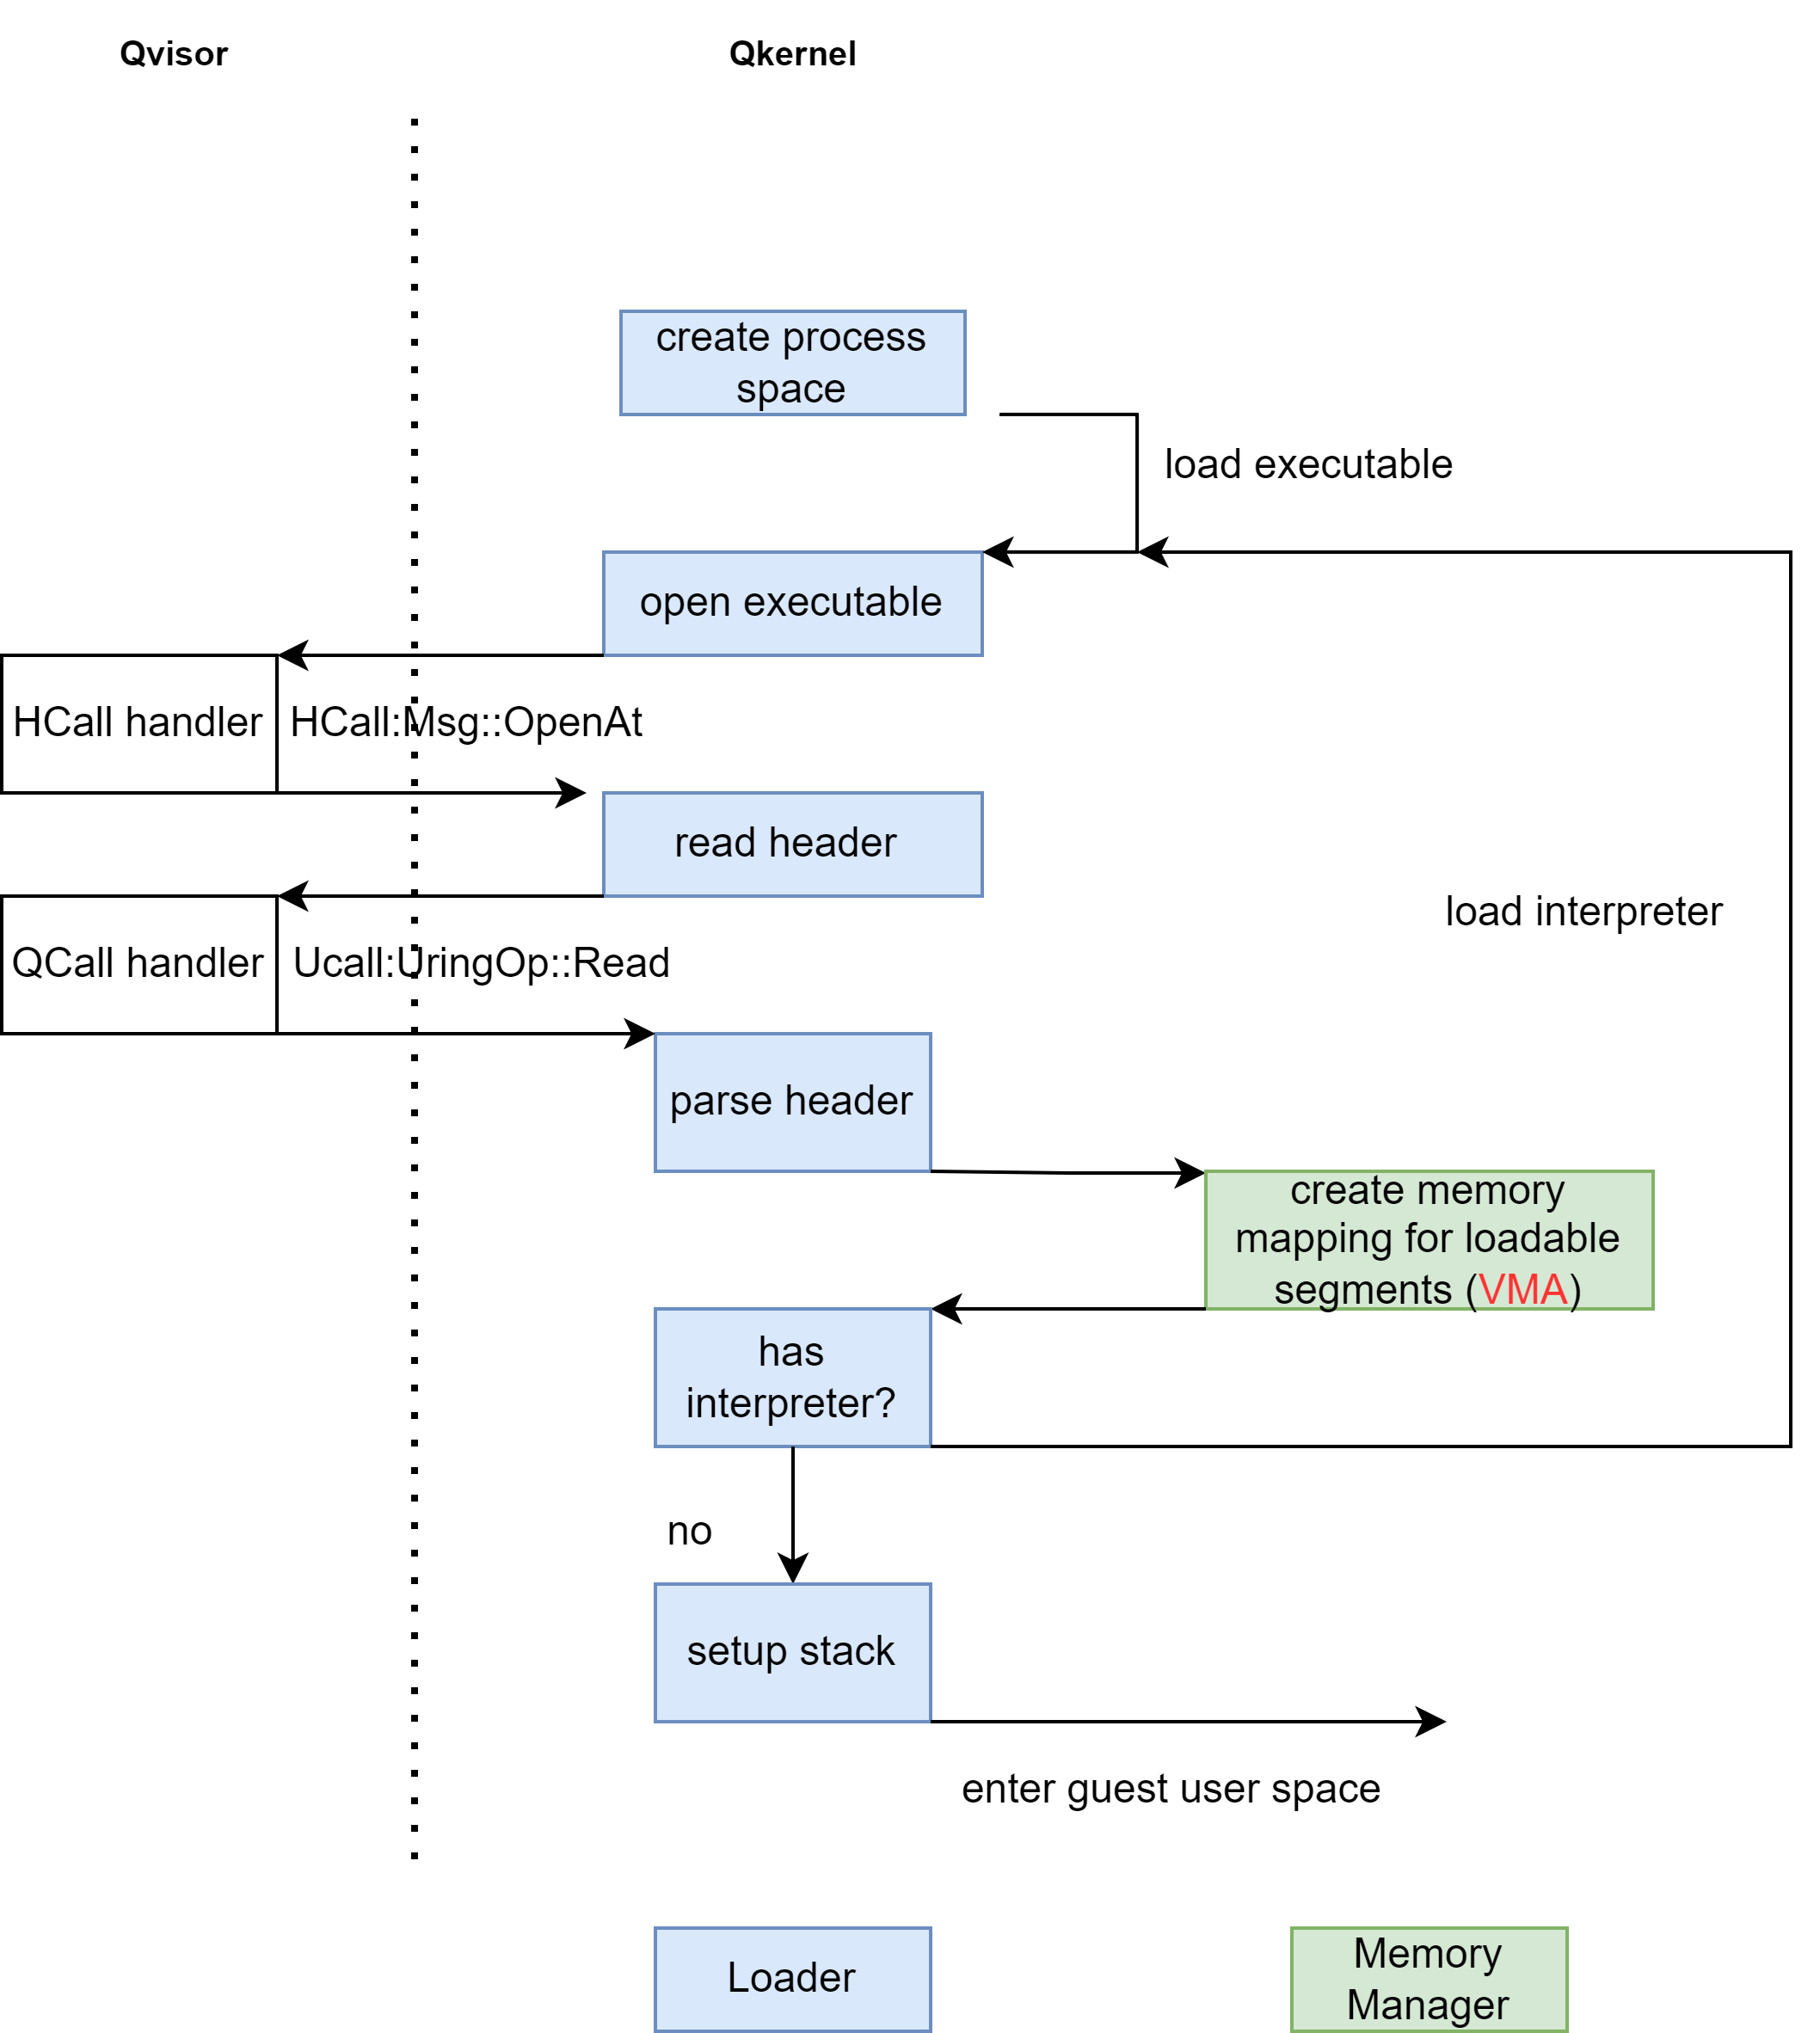
\includegraphics[width=0.9\linewidth]{images/loader_flow.png} 
    \caption{Loader setup Memory Mappings during Application Startup} 
    \label{fig2:a} 
    \vspace{4ex}
  \end{subfigure}%% 
  \begin{subfigure}[b]{0.5\linewidth}
    \centering
    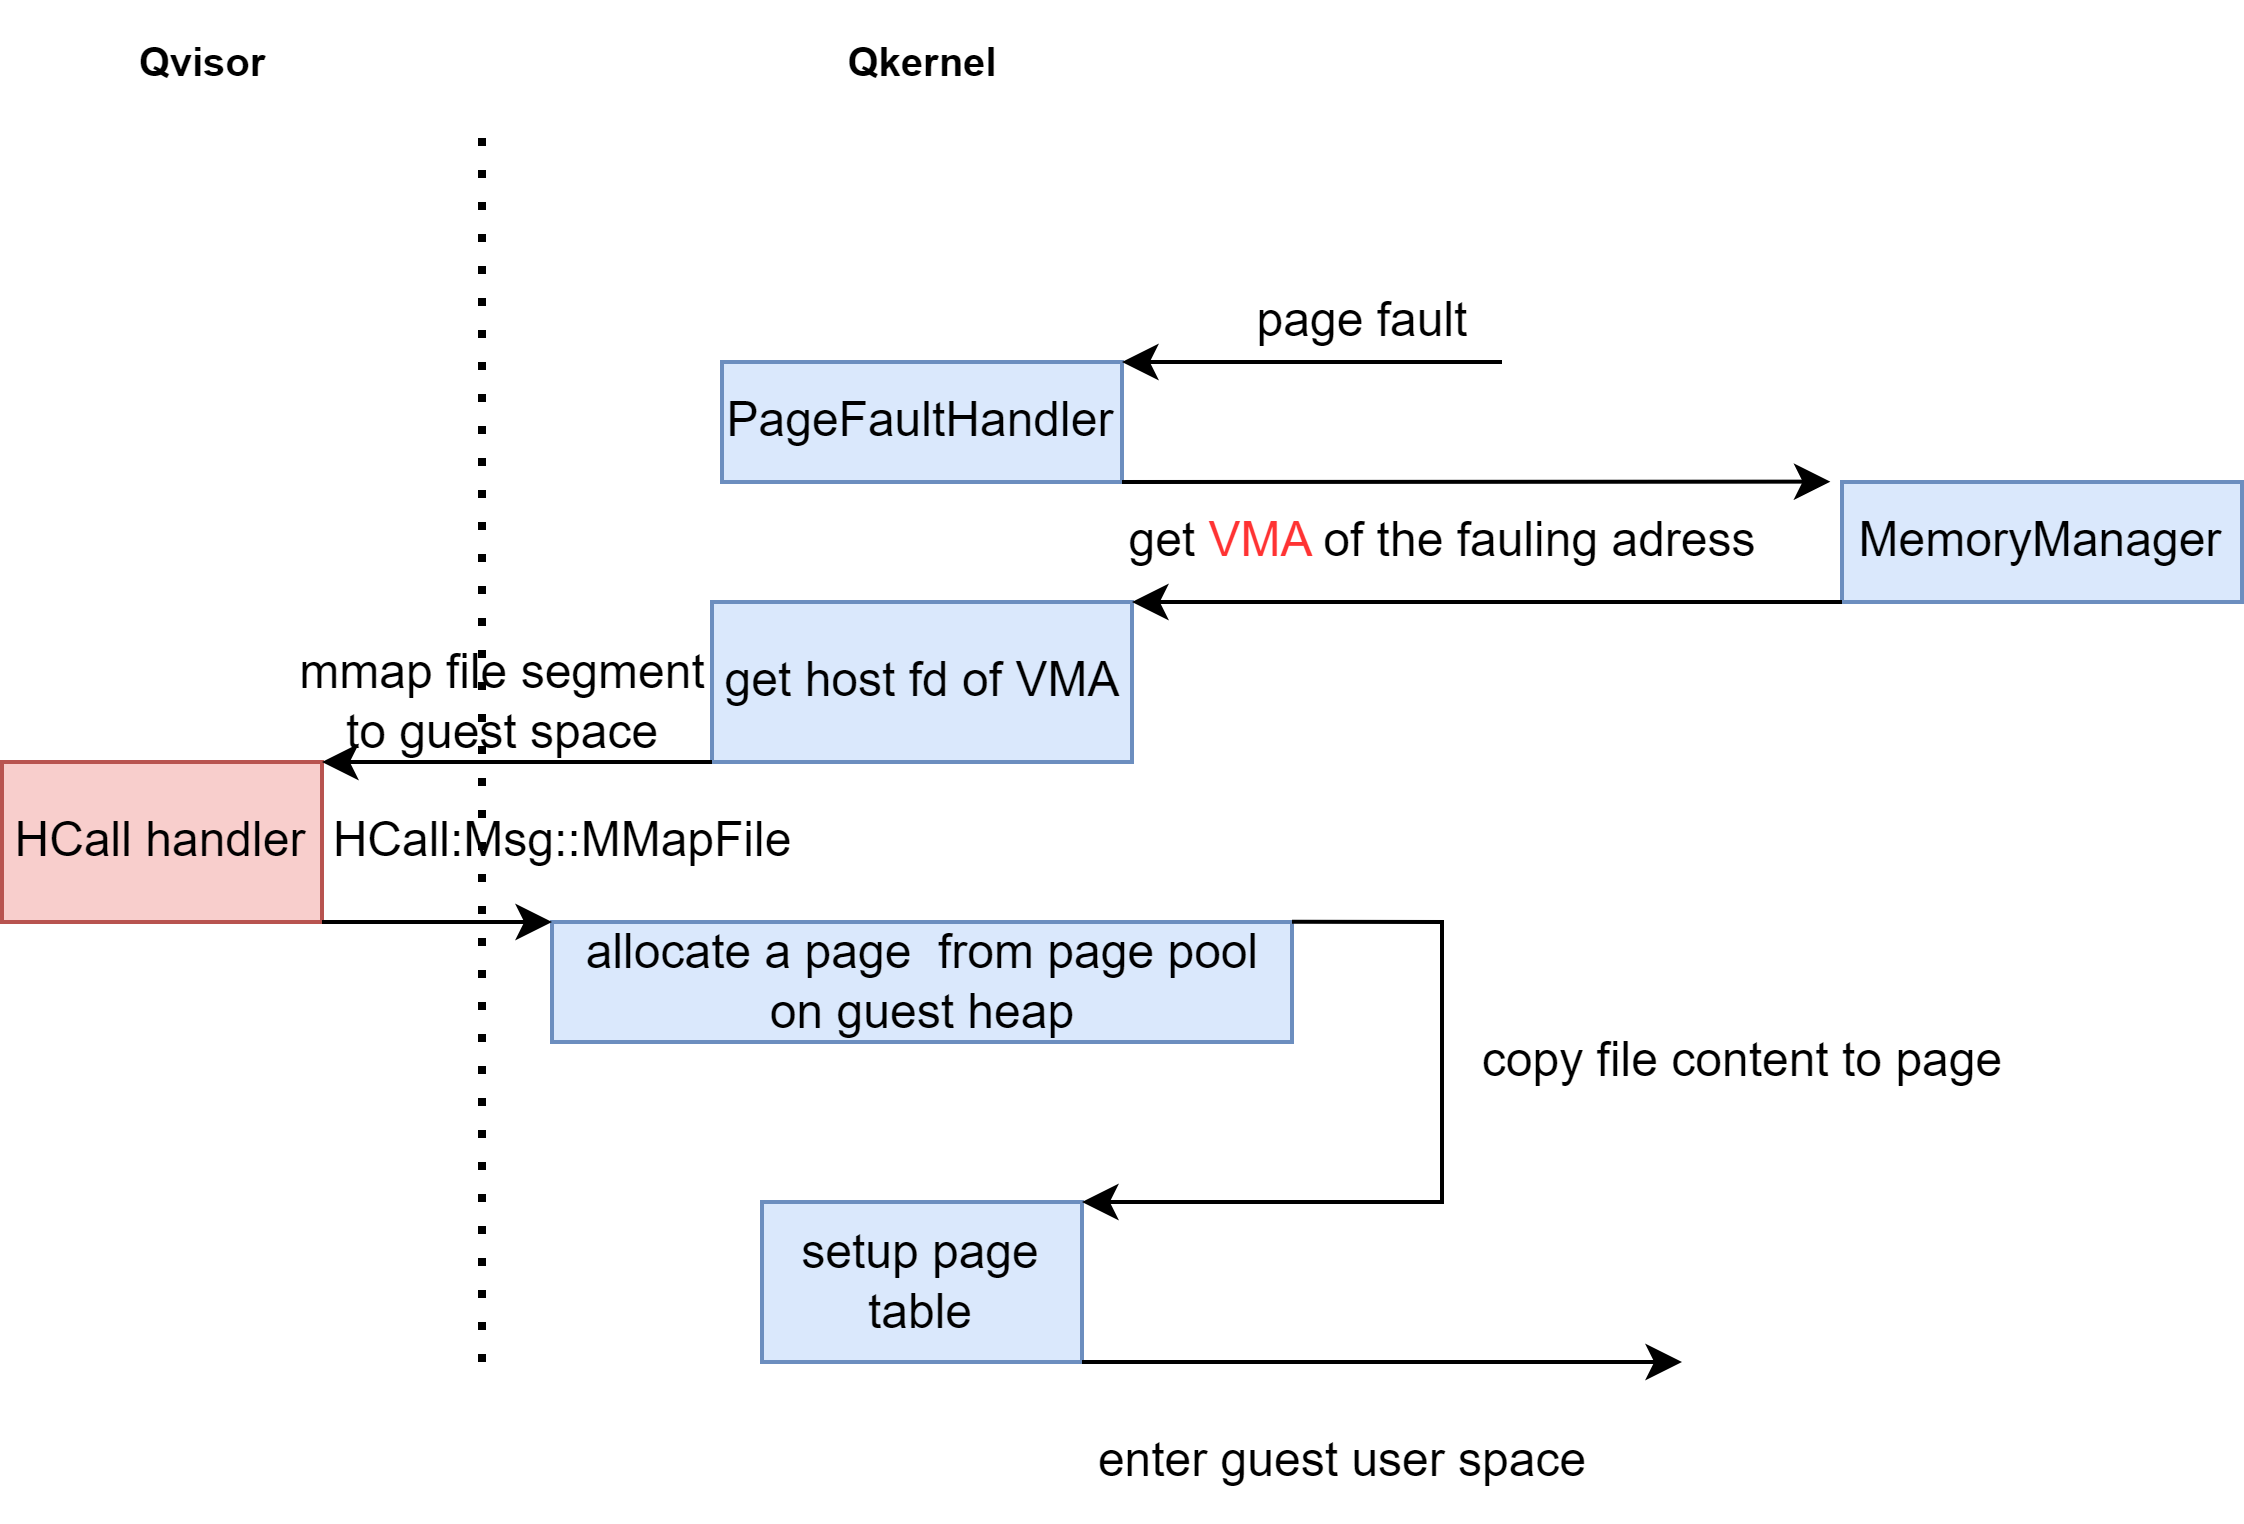
\includegraphics[width=0.9\linewidth]{images/page_fault_handling.png} 
    \caption{Page Fault Handling} 
    \label{fig2:b} 
    \vspace{4ex}
  \end{subfigure} 
  \caption{Application Binary Loading Process}
  \label{fig2} 
\end{figure}

\subsubsection{Loading compromised application binary during startup}
\label{sec:app_binary_loading}
The application binary is stored in the host's space. During the setup of the application process, the Qkernel loader opens the application binary using Hcall::Openat, reads its ELF header 
into the qkernel using the file Ucall::read, and then requests the Qkernel virtual memory manager to create a process image for the application, i.e., creating a private virtual memory area (VMA) for each loadable segment that is defined in the 
ELF file (Figure~\ref{fig2:a}). When the application process runs, accessing an address within the VMA will trigger a page fault. This is handled by the qkernel page fault handler. The workflow for the page fault handling can be found in FigureFigure~\ref{fig2:b}. Since the VMA of 
a loadable segment is private, the page fault handler uses hcall::mmap to request Qvisor to map the relevant loadable segment into the guest physical space, then allocate a page from the page pool on the Qkernel heap, and copies the contents of 
the segment from the guest physical address to this page. Finally, a page table entry (guest virtual address -> address of the page) is created and the page fault handling is done. The fact that the application binary is loaded from the host to 
the Qkenel makes it possible for an attacker to induce qkernel to execute the compromised code on the fly. For instance, the loader might request Qvisor to open binary A using Hcall::openat during application startup, but instead, untrusted Qvisor 
provides the descriptor of file B. As a result, the loader creates the wrong memory mapping, and consequently, the page fault handler will load the code from file B instead of file A. Furthermore, since the page fault handler uses Hcall::mmap to 
map the executable into the guest physical space, an attacker could manipulate the Qvisor to map compromised code into the guest physical space. In this case, the page fault handler simply copies this code to a page, creates a page table entry, 
and then returns to the application process without an integrity check. This leads to the execution of malicious code by the application. To mitigate this vulnerability, after the memory manager creates a VMA for a loadable segment, the Qkernel 
should immediately read the address range. This facilitates the page fault handler to load the segment into the guest before application runs. Also, the Qkernel should measure the read content simultaneously, then forward the measurement to relying 
party as part of the application launch measurement for integrity checking. To mitigate this vulnerability, Qkernel should read the address range and measure the read content immediately following the creation of a VMA for the loadable segment. 
By doing so, the page fault handler loads the binary into the qkernel before the application launch. The resulting measurements can then be forwarded to the relying party as part of the application startup measurements for integrity checking. 
In this way, we ensure the correctness of the application binary loaded into the qkernel.

\begin{figure}[H]
  \centering
  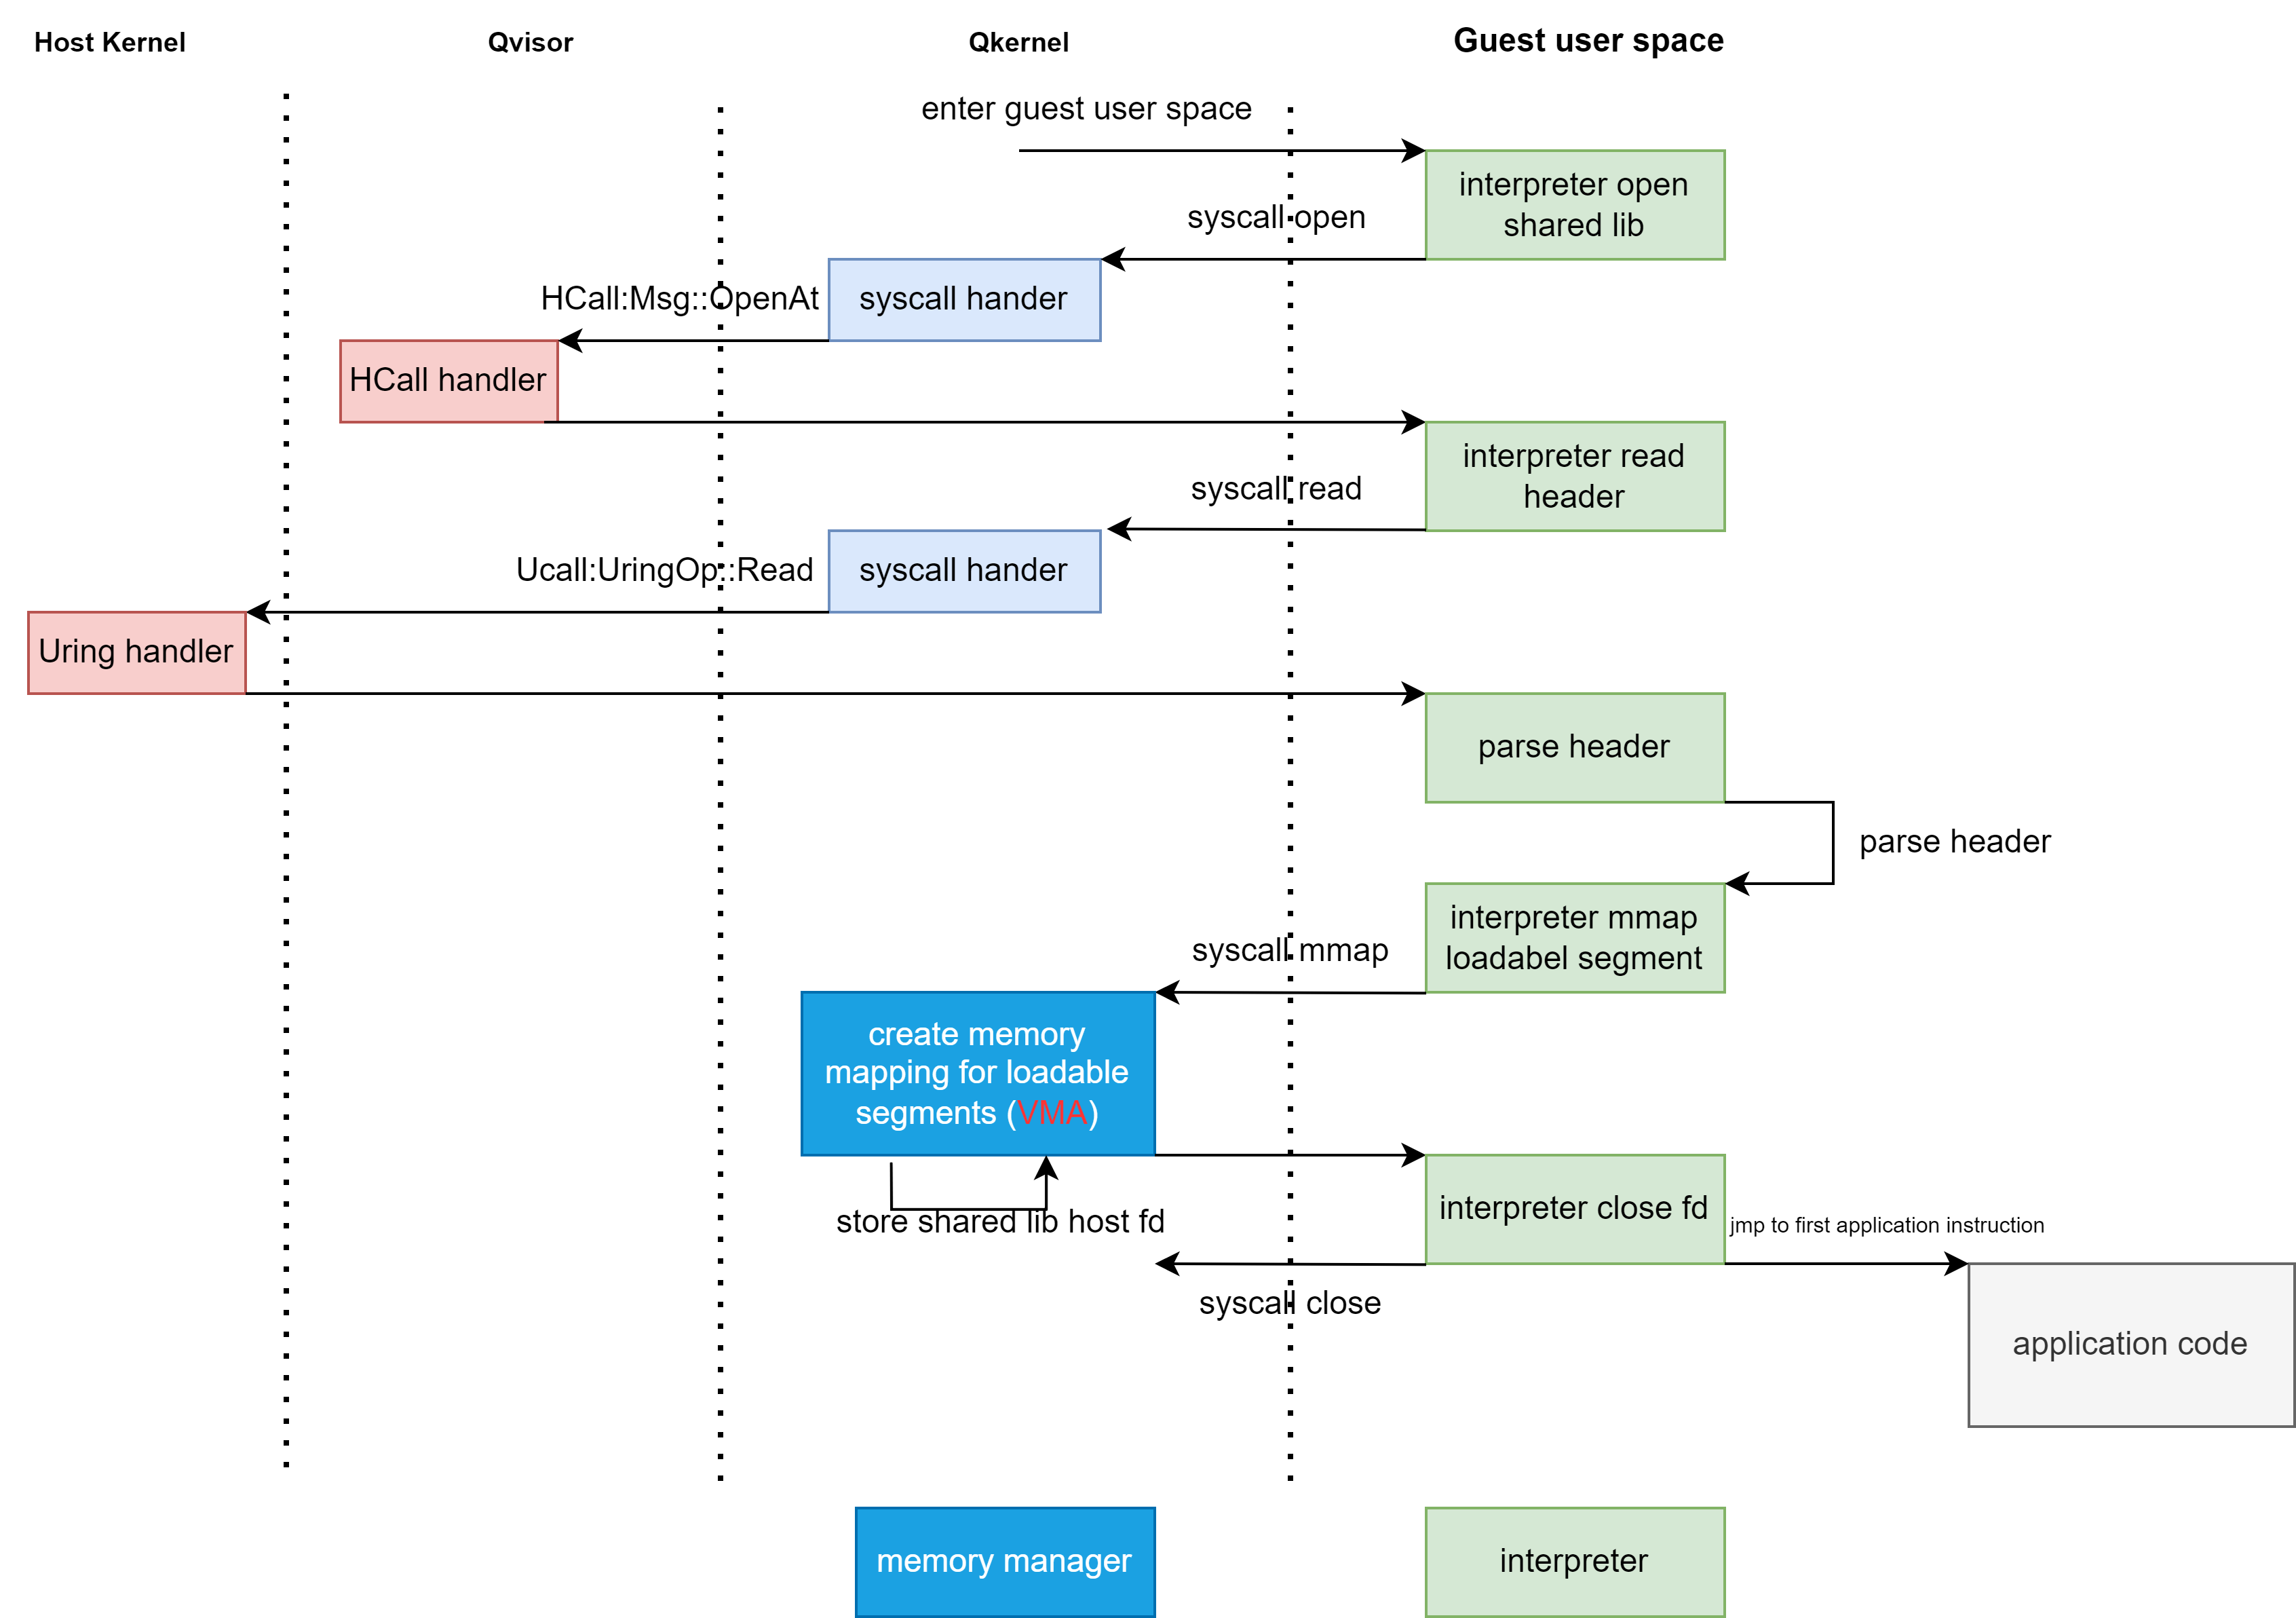
\includegraphics[width=1\textwidth]{images/load_shared_libarart.png}
  \caption[Interpreter setups shared library's memory mappings]{Interpreter setups shared library's memory mappings}
  \label{fig:load_shared_libarart}
\end{figure}


\subsubsection{Loading compromised binary at runtime}

Dynamic libraries are binary files stored on the host and loaded at application runtime by the interpreter. When the application is a dynamically linked executable, the interpreter's code is executed first upon the application process launched.  
As depicted in Figure~\ref{fig:load_shared_libarart}, the interpreter uses the open, read, and mmap system calls to create private memory mappings (VMA) for the loadable segments in the shared library.  Accessing an address within the VMA triggers 
page faults, and the page fault handler handles the fault in a manner similar to how it handles page faults when accessing the VMA of application binary segments.   Since the process of how the qkernel creates memory mapping and later loads code to 
the guest for shared library and application binary are very similar, the issues encountered in the previous section also apply here. To resolve the issues, the qkernel should measures the shared library by reading the VMA before mmap called by the interpreter 
returned. This prompts the page fault handler to load the library into the guest. However, since the library’ measuring happens after remote attestation, the qkernel does not forward the measurements to the relying party. Instead, it 
verifies these measurements against the reference hash in the policy file obtained from the relying party.

Executing a command at runtime will cause the qkernel to load the binary corresponding to that command. For example, for the exec command, as discussed in section xx, the quark-agent will load the binary consrepoding to the command and create 
a exec process. The binary loading mechanism has already been discussed in section~\ref{sec:app_binary_loading}. Therefore, a malicious user can take this opportunity to inject malicious code into the qkernel. The mitigation is similar to the previous section, where qkernel 
will measure the binaries loaded into qkernl and check the correctness of the loaded binaries using the reference hash of the binaries in the policy file obtained from the relying party.


\subsubsection{Lack of management of application restarts}

In the event of an unexpected application crash, Kubernetes may recreate a pod to execute the crashed application or restart the program within the original pod if the persists\cite*{k8s}. In the latter case, Qkernel reloads the application binaries 
and process specifications. from the host and provide the relaunched application with the secret obtained from relying party during the first startup. An attacker may use this opportunity to inject malicious code and process specifications into Qkernel, 
which causes an incorrect process setup or executing of compromised code. To mitigate this threat, Qkernel should measure the application recreation process and compare the measurement result with the initial application startup measurement stored 
on guest memory. If the 2 hashes don’t match,  Qkernel should panic.

\subsection{No restriction to the available System Calls for Applications}
Seccomp section in the OCI runtime specification\cite*{oci-spec} define a way for user to rescrict the available system calls for applications.  Unfortunately, Qkernel does not support seccomp\cite*{seccomp}. If a guest process is compromised, 
those unnecessary system calls can be abused to attack the qkernel and other processes. In the field of computer security, component hijacking\cite*{DBLP:journals/corr/WuGLD16} is an attack pattern in which an attacker can attack the kernel and other processes by hijacking a process and forcing it to execute a 
vulnerable system call. For example, an attacker can start a malicious exec process, which uses a vulnerable system call to steal application secrets stored in Qkernel. To this end, we implement a guest system call interceptor. The application 
owner is allowed to specify the available system calls for the application. 
For more details on the mitigation please refer to section XX.

\subsection{No control over guest kernel arguments}
\begin{figure}[H]
  \centering
  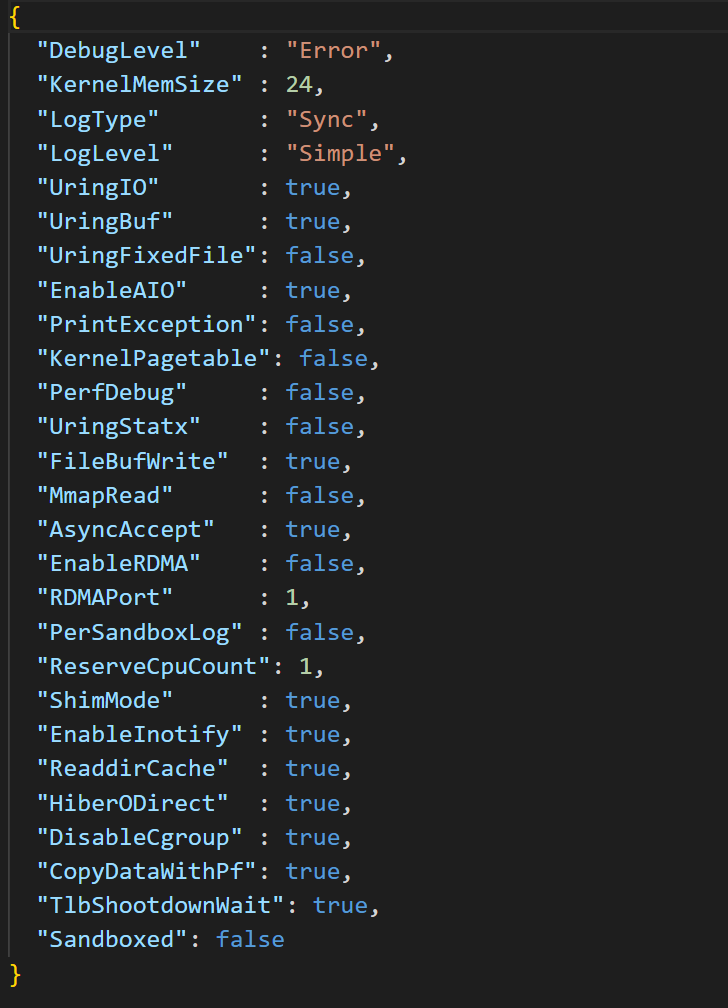
\includegraphics[width=0.5\textwidth,height=0.4\textheight]{images/quark_config.PNG}
  \caption[Configuration file for Qkernel, Qvisor, and Quark shim]{Configuration file for Qkernel, Qvisor, and Quark shim. The file is installed as a global configuration file for quark in the /etc/quark/ directory. When quark-shim or qvisor starts, it reads this file and completes the relevant configuration}
  \label{fig:quark_config}
\end{figure}

Qkernel is a binary which is loaded into the guest memory during Qvisor setting up the guest. To properly configure the Qkernel,  Qvisor also passes several command-line arguments to the Qkernel, including the number of vcpus, the socket file 
descriptor that the quark-agent listens to, and a configuration file shown in Figure~\ref{fig:quark_config}. This configuration file specifies the runtime behavior of the Qkernel, such as whether to enable the ucall interface, whether to enable RDMA, and so on. A malicious configuration 
files can lead to the disclosure of the secrets stored in Qkernel. For example, turning on RDMA would allow an untrusted remote party has the direct access to the Qkernel’s memory. For this reason, the Qkernel should measure the configuration file 
and send it as part of the application startup hash to the relying party for integrity checking. 

\subsection{Qkernel Log Misconfiguration}
Qkernel logs is stored by qvisor in the host /var/log/quark directory via Hcall::HYPERCALL\_PRINT. Currently, the Qkernel logging system supports five levels of logging, OFF, Error, Info, Debug, Trace. Here OFF is the minor level, i.e. the least 
detailed, and Trace is the highest level, i.e. the most detailed log. The user can configure the highest level of logging for qkernel through DebugLevel ketword in the configuration file (Figure~\ref{fig:quark_config}). For example, when the DebugLevel is info, qkernel 
prints logs in level error, and info. 

A malicious k8s administrator may set the DebugLevel keyword to Trace and then analyze the qkernel logs stored in the host to obtain sensitive information. 
This problem can be solved by measuring the guest kernel arg. However, both Qvisor and Qkernel are configured using this file. Specifically, Qvisor reads this configuration file after startup and pass a copy of it into the Qkernel as command 
line argument when lauching the guest. If the k8s administrator sets the DebugLevel keyword to trace in order to view the qvisor's logs, the Qkernel will have to print very detailed log messages, which may contain application’s secrets. 
To break the coupling between the qvisor and qkernel logging system configuration, we should offload the qkernel logging system configuration from this configuration file and allow the application owner to specify the maximum logging level of the 
Qkerenl logging system in a policy. This policy is obtained at application startup via remote attestation. Until then, the logging level of the qkernel is set to the default level OFF, i.e. no logs will be printed.



\section{Summary}
In this chapter, the threat model is first defined in section~\ref{sec:Threat_model}. Based on this model, the security issues in Quark are examined from various perspectives. These vulnerabilities found include:
\begin{itemize}
  \item Application secrets are managed and deployed by untrusted Kubernetes and Quark-shim
  \item Absence of end-to-end encryption for terminal data streams
  \item  Lack of cryptographic protection for application log
  \item Anyone can issue commands to an application
  \item Any user can allocate a terminal
  \item The commands issued by application owner may contain confidential data but are unprotected during transmission.
  \item Loading compromised application binary during startup
  \item Loading compromised binary/shared library at runtime
  \item Lack of management over application restart
  \item No restriction to the available system calls for applications
  \item No control over guest kernel arguments
  \item Guest kernel Log misconfiguration

\end{itemize}

% For this reason, we should offload the configuration of the logging system from the qkernel configuration file and allow the application owner to specify the maximum logging level for the specified client kernel logging system in the protection 
% policy.
\cleardoublepage

%%% Local Variables:
%%% TeX-master: "diplom"
%%% End:

% \chapter{Design}
\label{sec:design}

% Ist das zentrale Kapitel der Arbeit. Hier werden das Ziel sowie die
% eigenen Ideen, Wertungen, Entwurfsentscheidungen vorgebracht. Es kann
% sich lohnen, verschiedene Möglichkeiten durchzuspielen und dann
% explizit zu begründen, warum man sich für eine bestimmte entschieden
% hat. Dieses Kapitel sollte - zumindest in Stichworten - schon bei den
% ersten Festlegungen eines Entwurfs skizziert werden.
% Es wird sich aber in einer normal verlaufenden
% Arbeit dauernd etwas daran ändern. Das Kapitel darf nicht zu
% detailliert werden, sonst langweilt sich der Leser. Es ist sehr
% wichtig, das richtige Abstraktionsniveau zu finden. Beim Verfassen
% sollte man auf die Wiederverwendbarkeit des Textes achten.

% Plant man eine Veröffentlichung aus der Arbeit zu machen, können von
% diesem Kapitel Teile genommen werden. Das Kapitel wird in der Regel
% wohl mindestens 8 Seiten haben, mehr als 20 können ein Hinweis darauf
% sein, daß das Abstraktionsniveau verfehlt wurde.

%\ldots design \ldots

%\todo{write design}

In this chapter, a shielding layer design will be presented to mitigate the pitfalls found in Chapter~\ref{sec:security_analyse}. It consists of the following components:

\textbf{Remote attestation and secret provisioning Infrastructure.} This infrastructure provides a mechanism for securely deploying sensitive user data. Secret management and deployment are offloaded from Kubernetes and Quark Shim to the secret manager. Shield relies on this infrastructure to prove its 
identity to the secret manager and retrieve secrets in a secure manner. This infrastructure addresses vulnerability~\ref{vulnerabilities:1} identified in Chapter~\ref{sec:security_analyse}.

\textbf{Enclave Runtime Measurement.} The module measures the data loaded from the host after the enclave has booted, including binaries, shared libraries, Qkernel's configuration file, and the secret manager's public key. The resulting measurements extend different hashes, including the enclave startup hash, the application startup hash, the runtime binary hash, and 
the application restart hash. The enclave utilizes these hashes to perform integrity checks on the loaded data. As a result, weaknesses ~\ref{vulnerabilities:7}, ~\ref{vulnerabilities:8}, ~\ref{vulnerabilities:9}, and ~\ref{vulnerabilities:11} are mitigated.
 
\textbf{A new pattern for EXEC requests.} This pattern effectively addresses the following pitfalls identified in Chapter~\ref{sec:security_analyse}: issuing unauthorized commands to applications, unrestricted allocation of terminals using kubectl exec -it, and the lack of protection for commands issued by application owners.

\textbf{A mechanism for protecting guest processes' STDIO.} This mechanism ensures the confidentiality and integrity of the STDIO stream of interactive and non-interactive processes. In this case, application logs, execution results of privileged commands, and terminal data streams belonging to the application owner are protected. As such, weaknesses~\ref{vulnerabilities:2}, ~\ref{vulnerabilities:3}, and~\ref{vulnerabilities:5} are solved.

\textbf{System Call Interception and Qkenrel Log Management.} They propose a user-configurable guest system call interception and guest log protection policy to mitigate vulnerabilities~\ref{vulnerabilities:10} and~\ref{vulnerabilities:12}, respectively.
 
In the following, we first give an overview of the architecture in Section~\ref{sec:General_Architecture}. Then, we introduce the remote authentication and provisioning infrastructure in Section~\ref{sec:design_Quark_Attestation_and_Provisioning_Infrastructure}. Subsequent Sections~\ref{sec:Enclave_Runtime_Measurement},~\ref{sec:design_EXEC_Requests},
~\ref{sec:design_STDIO_PROTECTION}, ~\ref{sec:design_STDIO_PROTECTION}, ~\ref{sec:design_Interceptor}, and ~\ref{sec:Qkernel_logger}, we explain the new paradigm for EXEC requests, the 
mechanism for protecting the standard IO of guest processes, the guest system call interceptor, and the guest log management policy, respectively. Finally, we propose modifications to the OCI runtime interface in Section~\ref{sec:Modification_OCI}.


\section{General Architecture}
\label{sec:General_Architecture}
\begin{figure}[!htb]
    \centering
    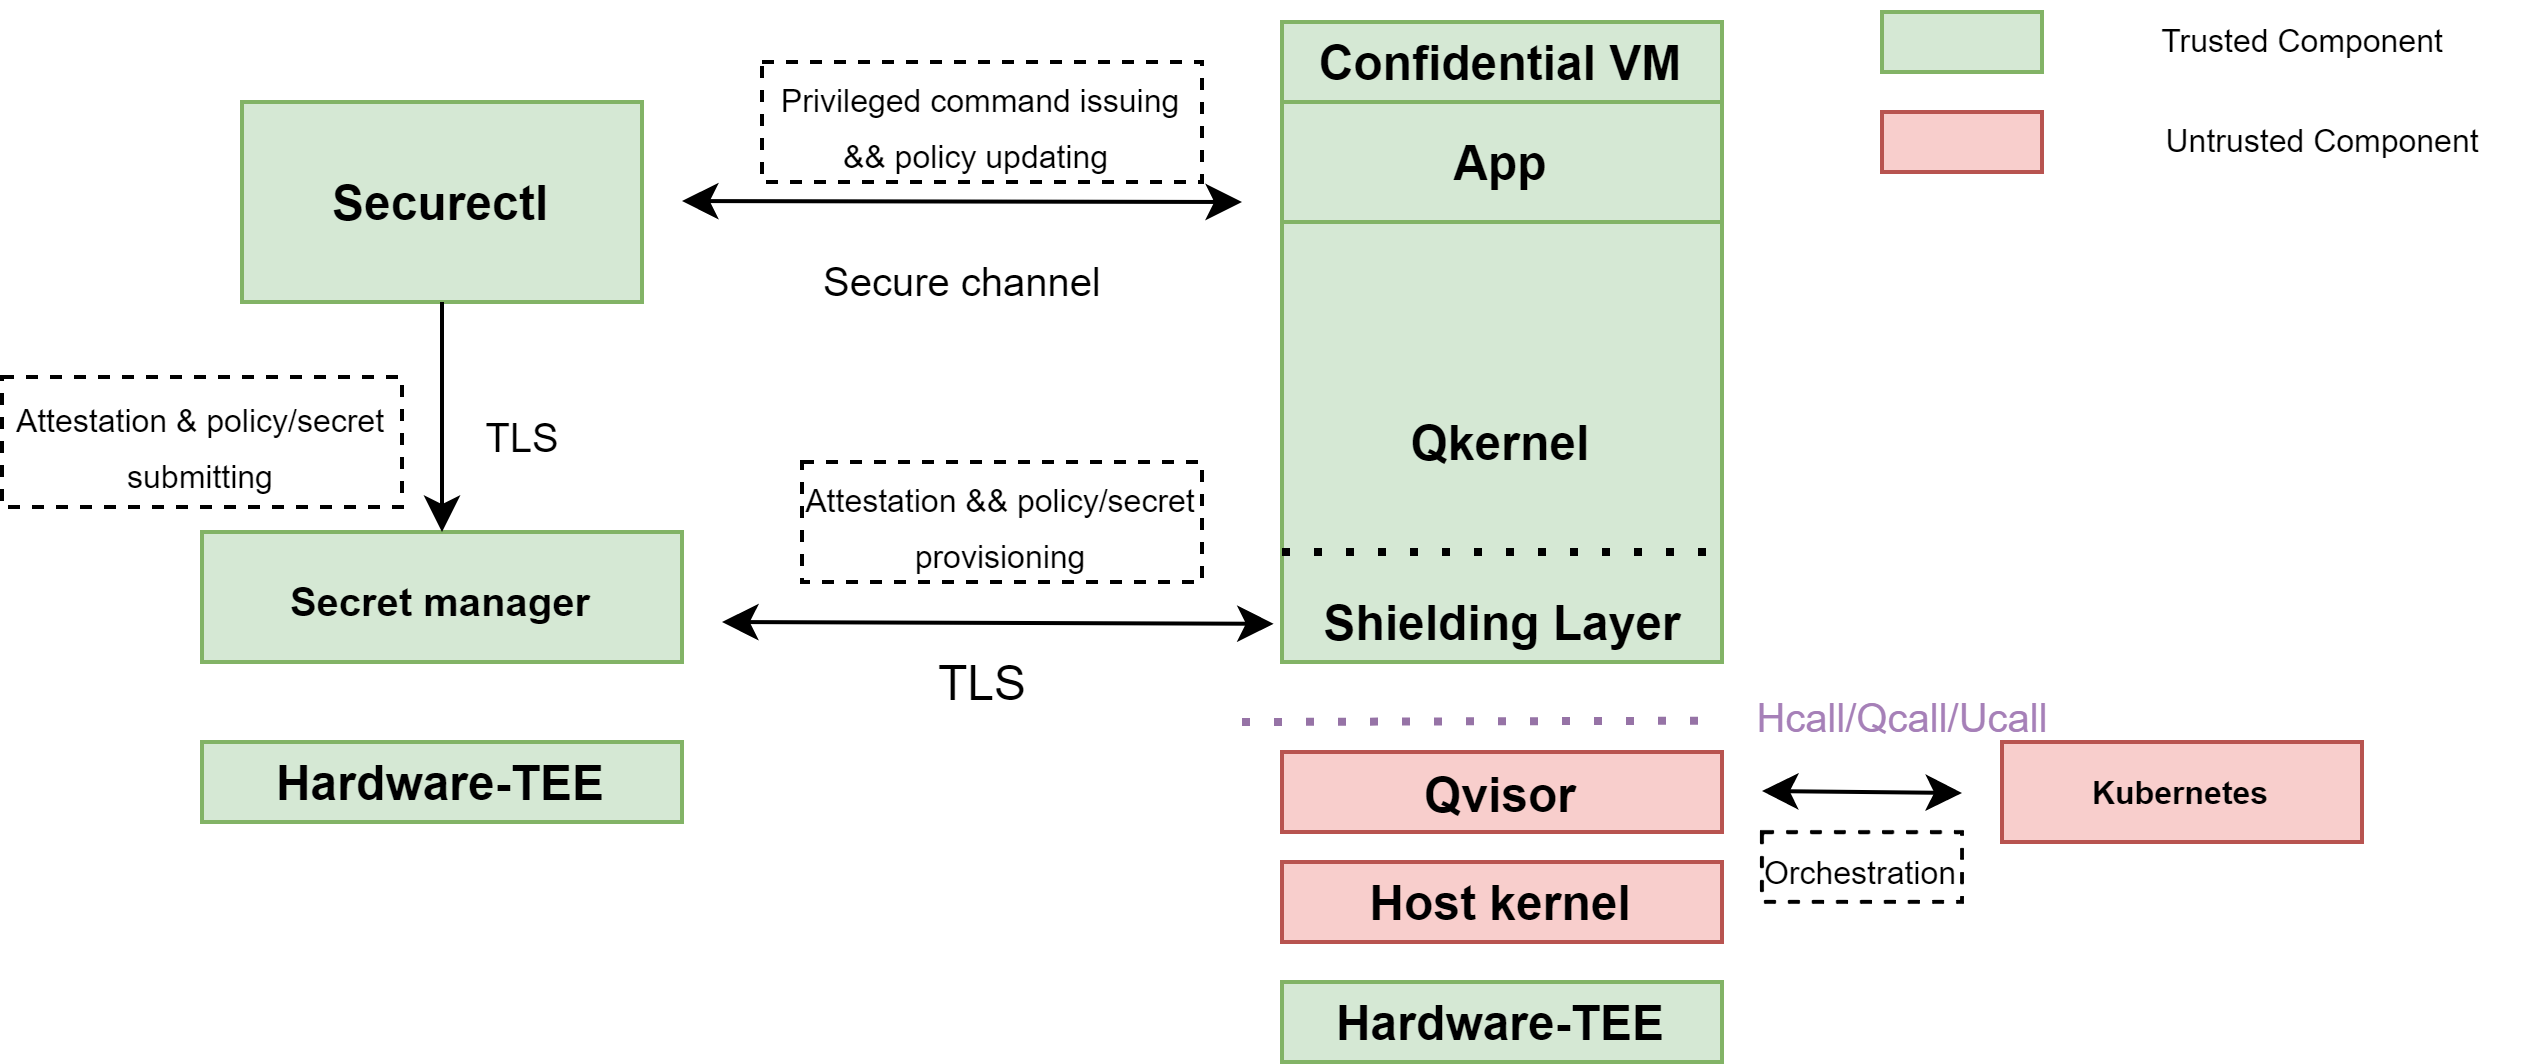
\includegraphics[height=0.3\textheight, width=1\textwidth]{images/genaral_architechture.png}
    \caption[General Architecture]{General Architecture. The green components in the figure are trusted ,and the red components are not trusted.}
    \label{fig:genaral_architechture}
\end{figure}
\todo{fix figure typo issue}

As shown in Figure~\ref{fig:genaral_architechture}, a secure virtual machine provides a trusted execution environment that encapsulates the guest, including the Qkernel and applications. This environment is also referred to as an "enclave." Notably, a shielding layer is added to the Qkernel to prevent adversaries from utilizing the Hcall, Qcall, and Ucall interfaces to launch attacks 
on the enclave. As this shielding layer is part of the Qkernel, its state is protected by the secure virtual machine.

We introduce Securectl for enclave owners. This tool runs in the enclave owner's local environment and provides an interface to interact with the application and control the shielding layer. The secret manager manages application secrets and runs in a confidential VM on the cloud. The enclave owner can authenticate the Secret Manager using remote attestation 
and then uploads secrets through a secure channel. The secret manager can validate the application startup process against the policy uploaded by the application owner and securely sends secrets to the enclave. The shielding layer is responsible for secret deployment and ensures that secrets are not disclosed while the enclave runs.


\section{Quark Attestation and Provisioning Infrastructure}
\label{sec:design_Quark_Attestation_and_Provisioning_Infrastructure}

\begin{figure}[!htb]
    \centering
    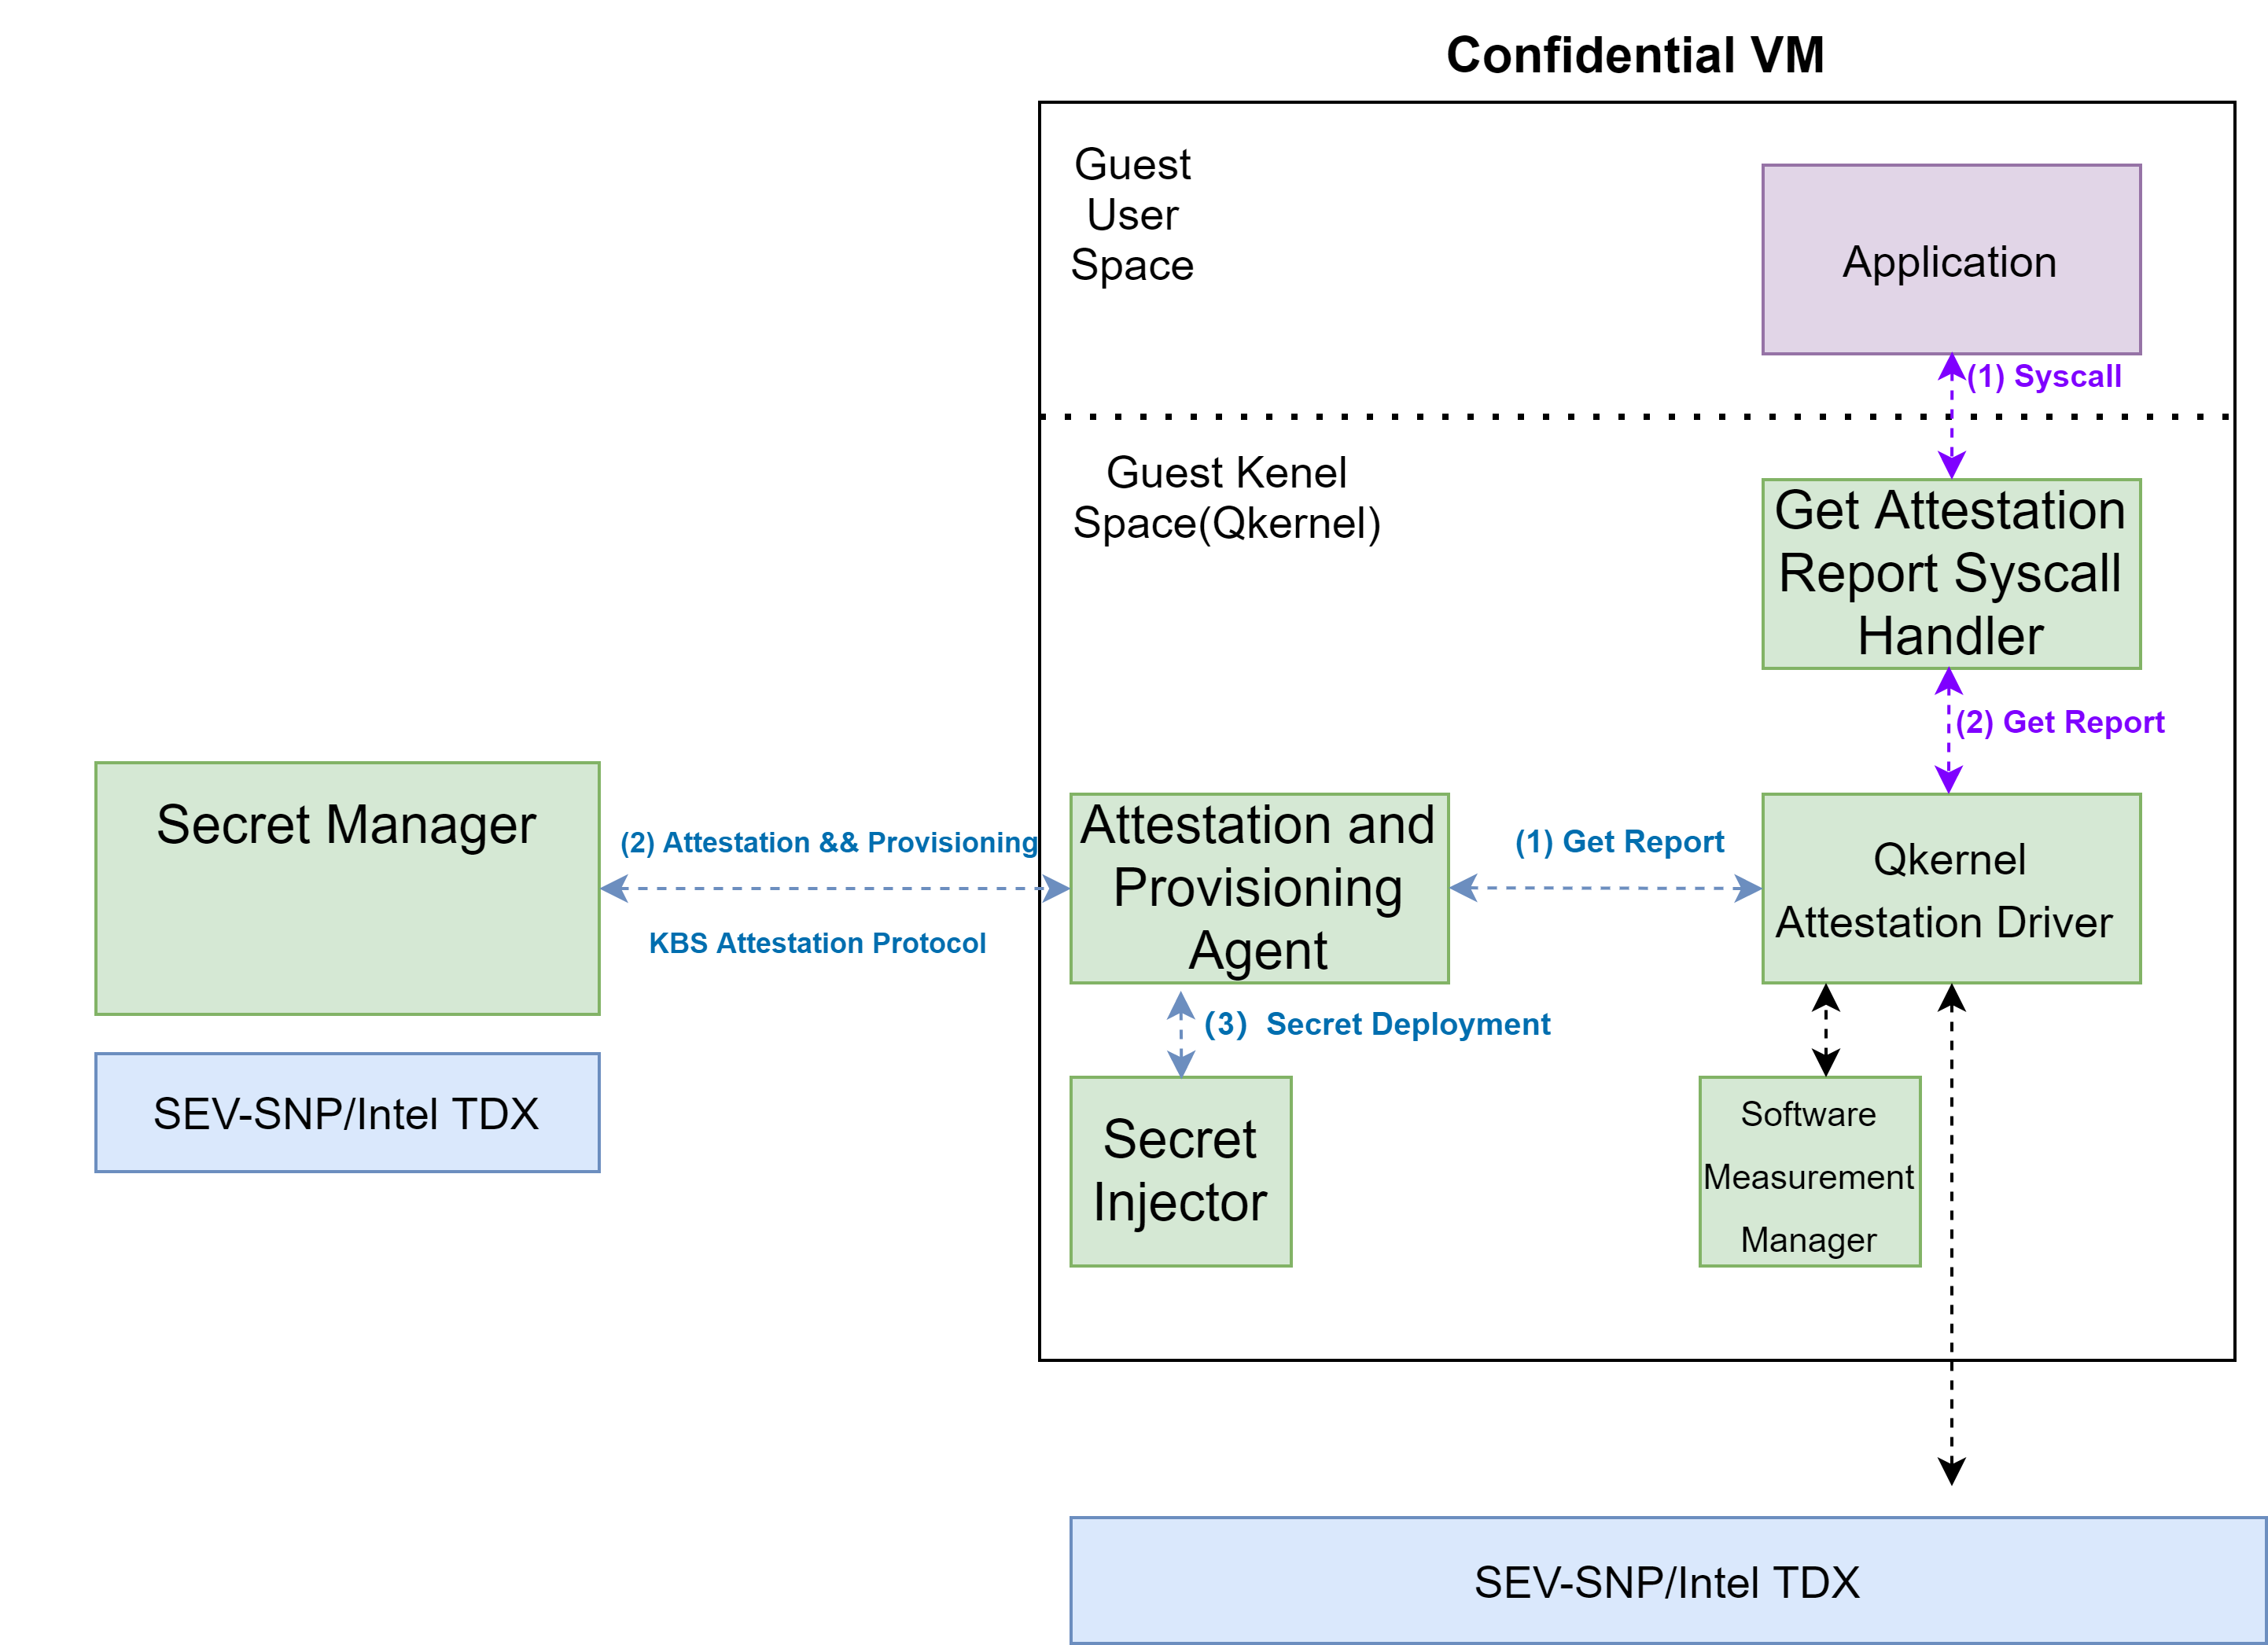
\includegraphics[width=0.8\textwidth]{images/Qkernel_attestation_infrastructurc.png}
    \caption[Quark Attestation and Provisioning Infrastructure]{Quark Attestation and Provisioning Infrastructure}
    \label{fig:Qkernel_attestation_infrastructurc}
\end{figure}

The Quark attestation and provisioning infrastructure consists of the modules in green in Figure~\ref{fig:Qkernel_attestation_infrastructurc}. It provides the following services for an enclave:

This infrastructure enables the secure deployment of secrets during application startup. Before the application process is launched, the remote attestation and provisioning agent uses the KBS attestation protocol to prove its identity to the secret manager and retrieve secrets. These secrets include shield policy, application startup parameters, environment 
variables, and files. The TEE hardware generates the attestation report required in the protocol with the help of the Qkernel attestation driver. This report contains the enclave startup hash. This hash includes measurements made by the software measurement manager on data loaded from the host, such as application binaries and Qkernel configuration files. 
The secret manager will compare the enclave startup hash with reference values provided by the enclave owner to ensure that the application and enclave are correctly configured. Once obtained secrets, the shielding layer is initialized according to the policy. The application's secrets are deployed to the application process by the secret injector. 
For instance, application startup parameters and environment variables are inserted into the stack of the application process. For file-type secrets, the injector keeps them on enclave memory and creates a sub-filesystem using the Qkernel's virtual filesystem interface. This filesystem is mounted in the /secret directory, and applications can access the secret files through this file system. In this way, we offloaded secret management and deployment from Kubernetes.

Additionally, The infrastructure allows applications to obtain attestation reports at runtime through the guest system call interface. For more information, please refer to Section~\ref{sec:runtime_attesation}.

This section is divided into three parts. Subsection~\ref{sec:design_Secret_Uploading} provides an overview of securely uploading secrets to the secret manager. Subsequently, in Sections~\ref{sec:secure_application_deployment} and~\ref{sec:runtime_attesation}, we discuss the secure deployment of secrets during application startup and how applications can request attestation reports at runtime, respectively. For specific implementations of each module, 
please refer to Chapter~\ref{sec:implementation}.
\begin{figure}[!htb]
    \centering
    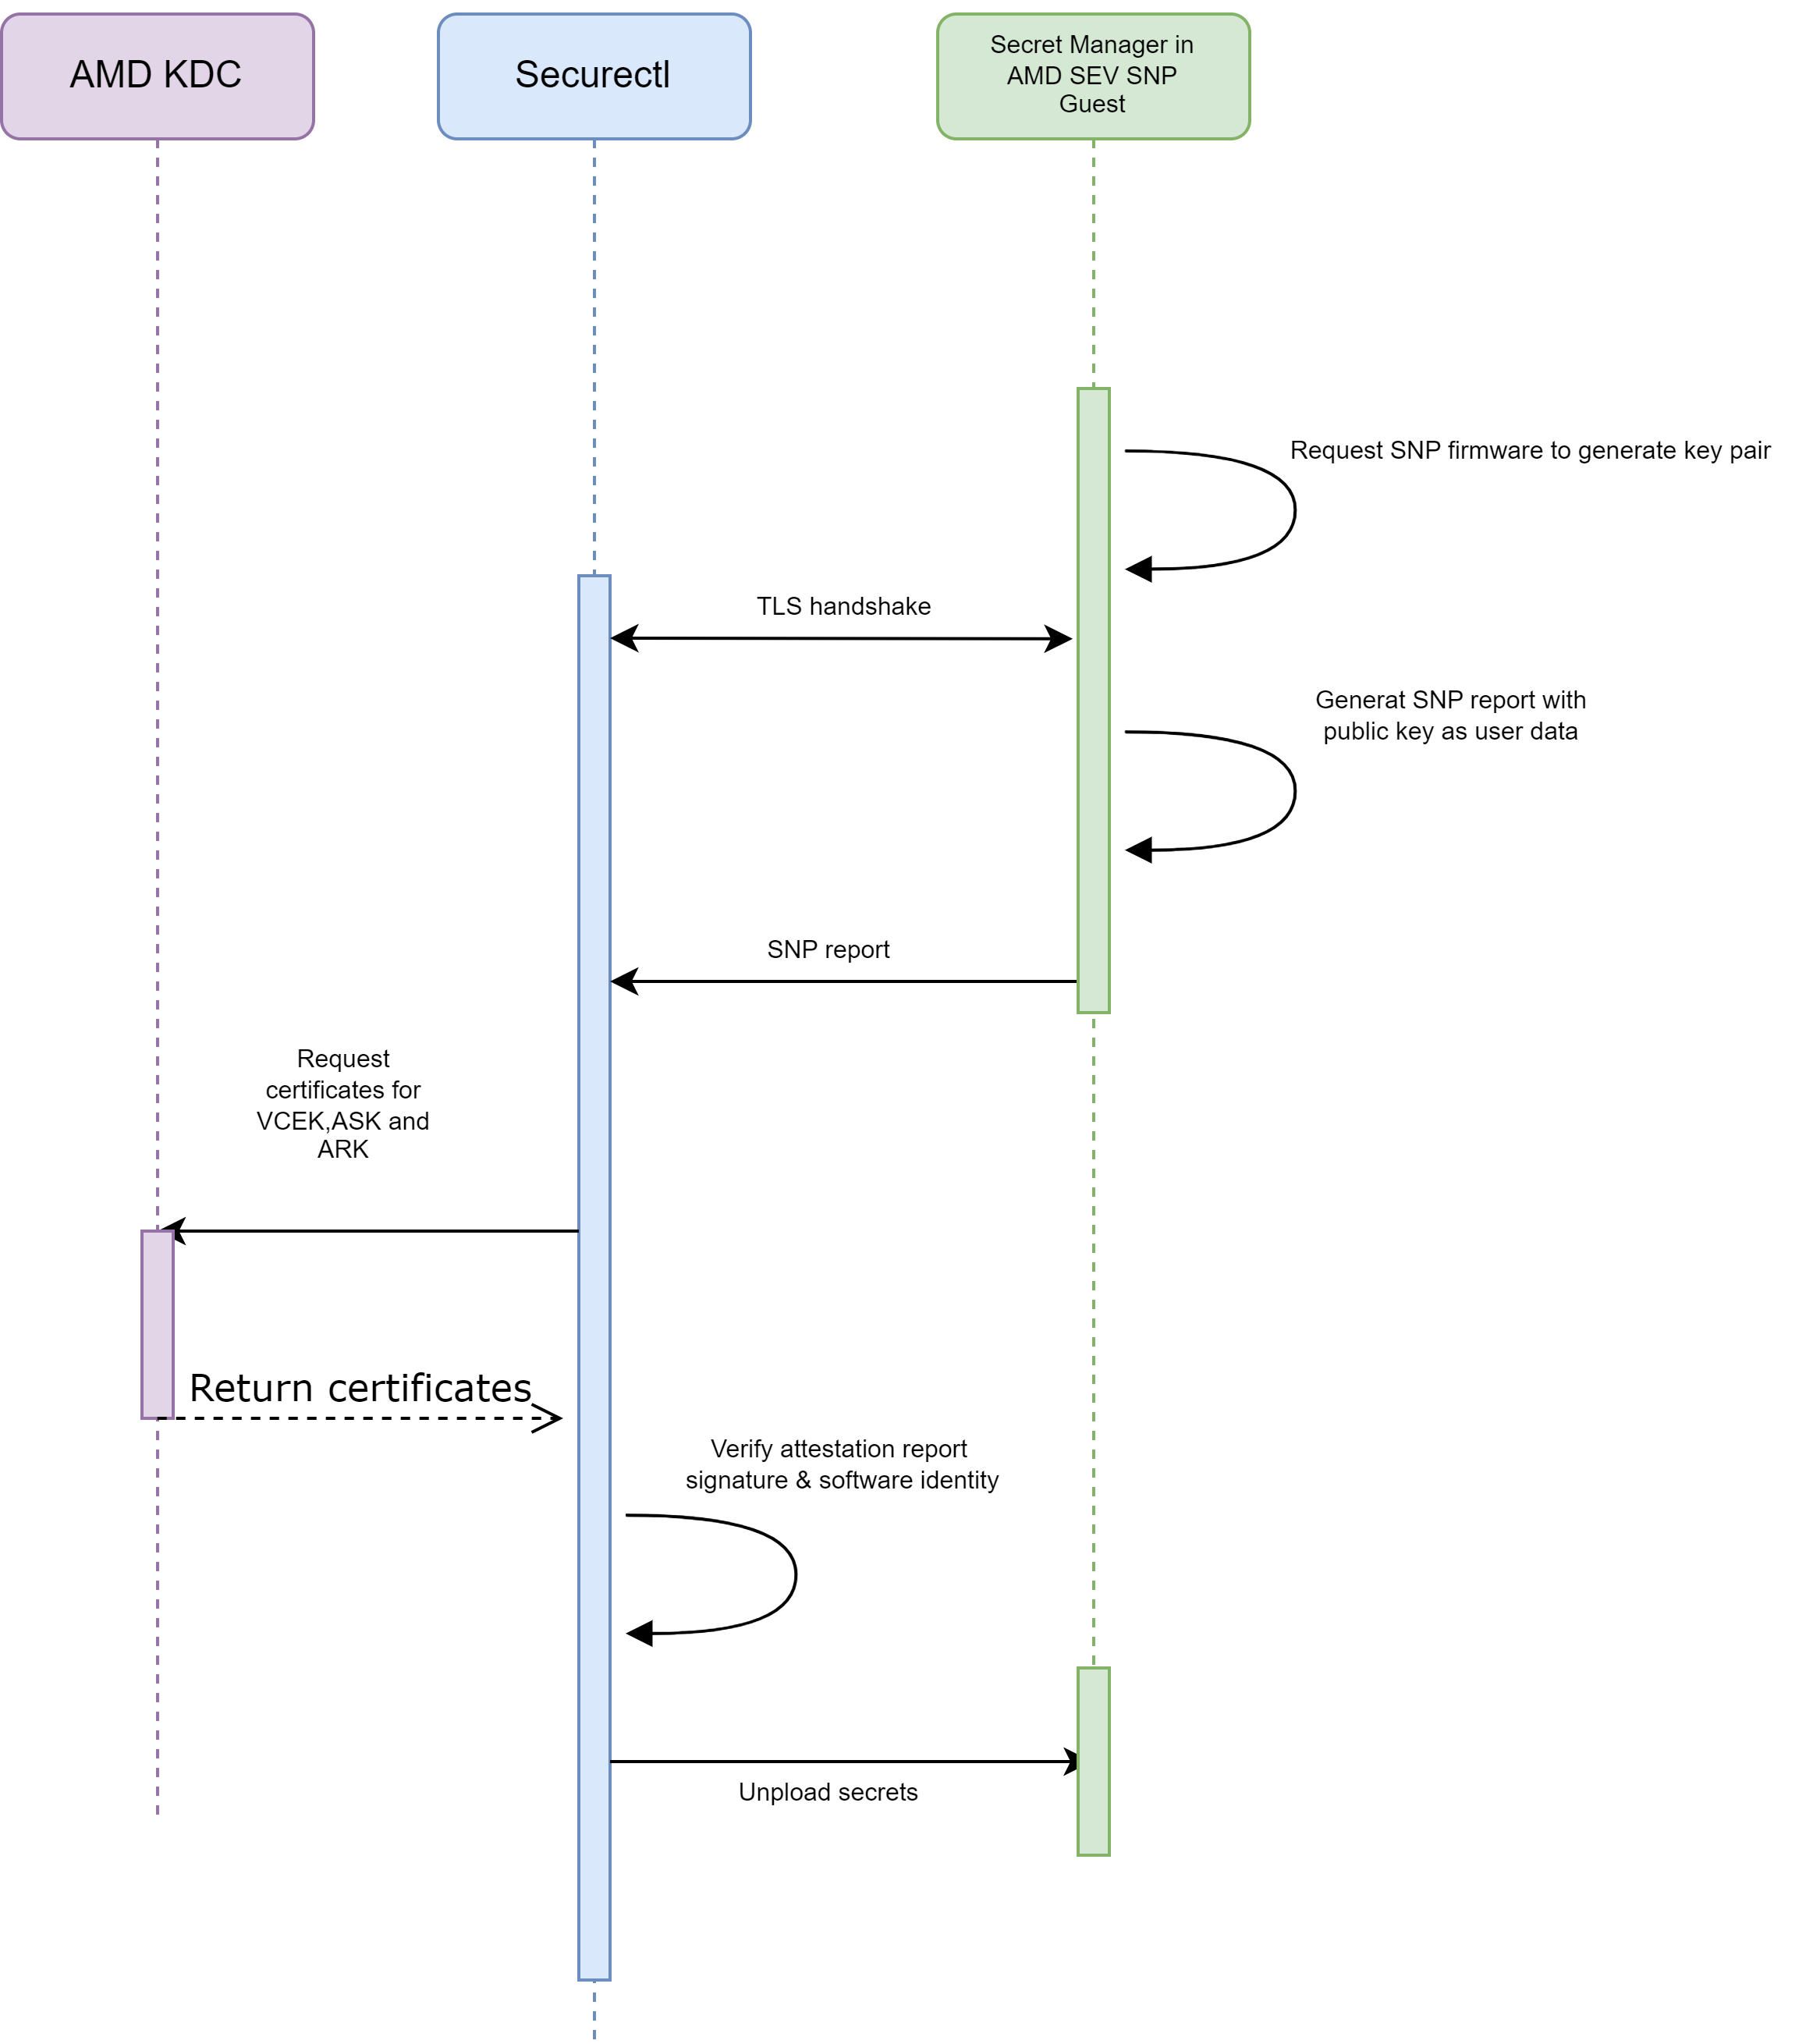
\includegraphics[height=0.4\textheight]{images/upload_secret.png}
    \caption[Secret Uploading Workflow]{Secret Uploading Workflow.}
    \label{fig:upload_secret}
\end{figure}

\subsection{Secret Uploading}
\label{sec:design_Secret_Uploading}
The process of uploading secrets to the secret manager requires two steps to be taken by the application owner. Firstly, the application owner needs to attest the secret manager. Secondly, a secure channel must be established for the secret uploading. This process is illustrated in Figure~\ref{fig:upload_secret}. We assume the secret manager is running in the AMD SEV SNP~\ref{fig:upload_secret}. 
Initially,the secret manager generate an RSA key pair for the TLS connection and store the private key in its memory. This key can be regarded as an identifier for the secure channel. To bind the secret manager to the identifier of the secure channel, the hash of the public key is added to the attestation report of the secret manager. Upon receiving the report, 
the application owner requests a certificate chain from the AMD KDC~\cite*{snp_kdc}. The certificate chain is then used to verify the signature of the report. Then using the information in the report, the application owner can ensure that the secret manager is genuine and that the hash of the public key used to establish the TLS matches the hash of the public key 
in the report. By fulfilling these steps, the application owner can determines that the entity on the other side of the secure channel is an expected secret manager. Thus, the channel can safely be leveraged for the secrets uploading.


\subsection{Secure Application Deployment}
\label{sec:secure_application_deployment}
\begin{figure}[!htb]
    \centering
    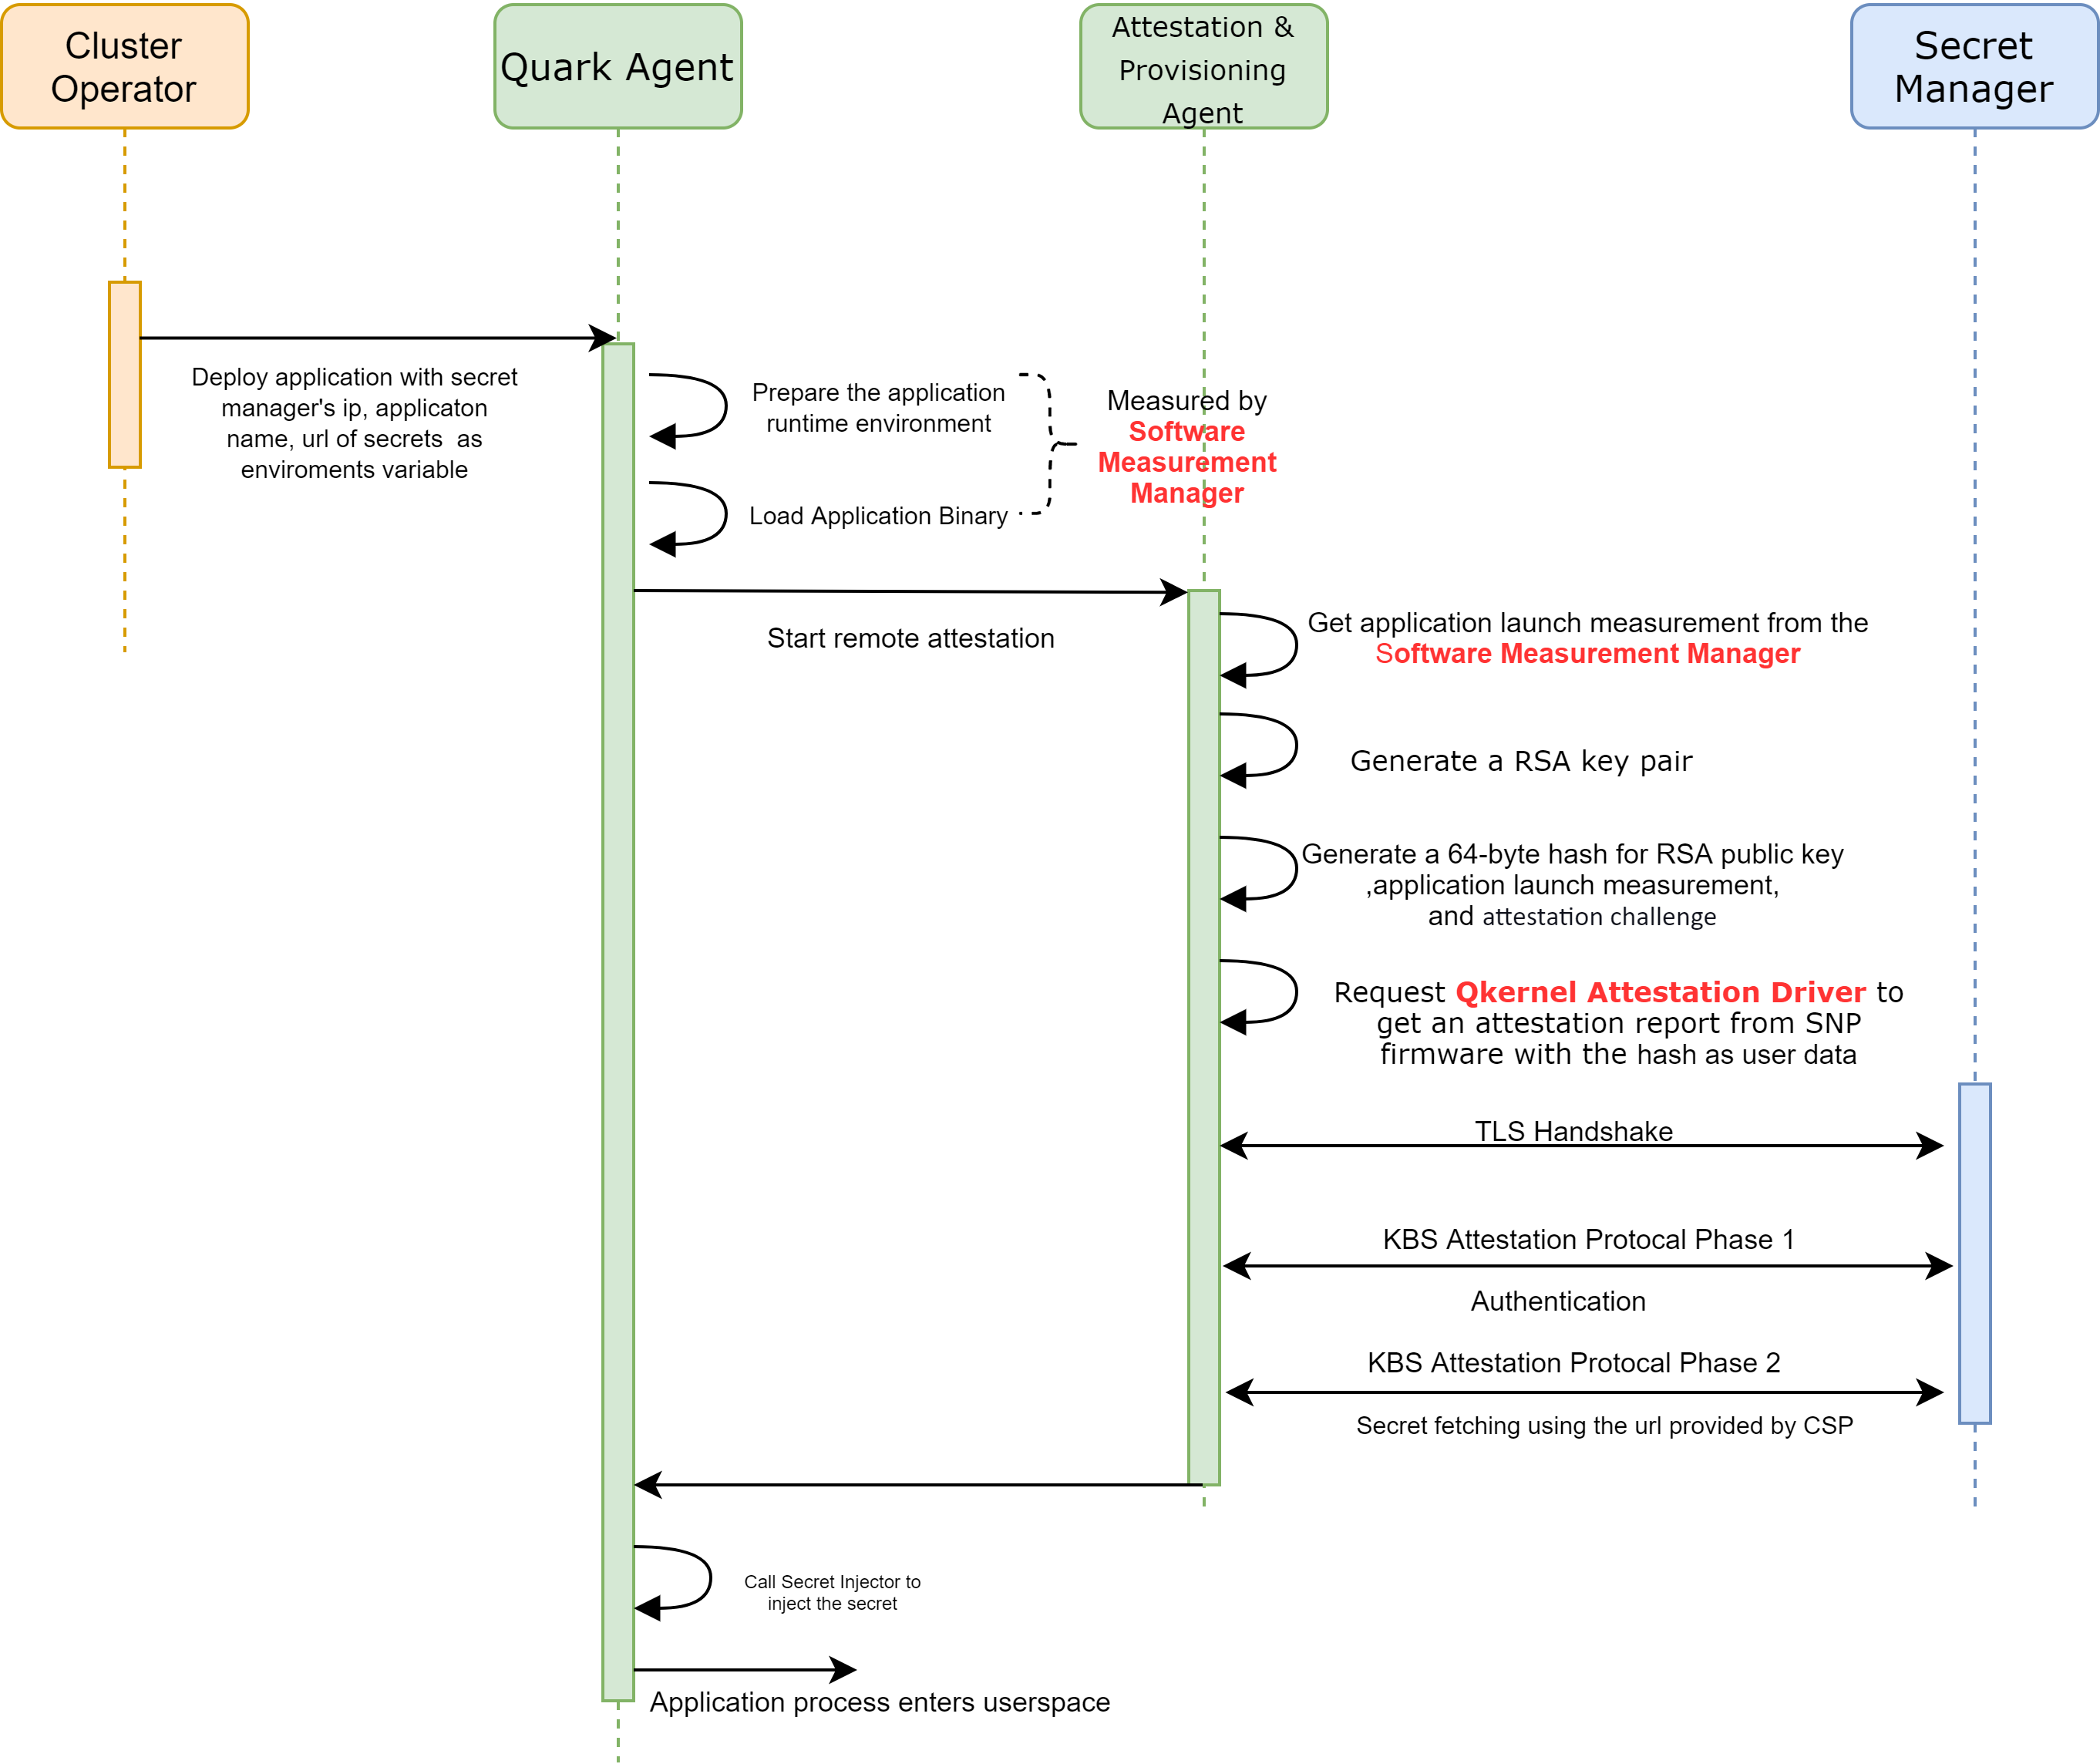
\includegraphics[height=0.5\textheight]{images/attestation_provisioning.png}
    \caption[Secure Application Deployment Workflow]{Secure Application Deployment. The green components are running in the enclave. The cluster operator is not trusted. The secret manager is responsible for managing the secrets, attesting enclaves, and provisioning the secrets.}
    \label{fig:attestation_provisioning}
\end{figure}

Secure application deployment aims to ensure the confidentiality and integrity of an application's sensitive data and the shielding layer's policy. We propose a new deployment mechanism to achieve this goal, as illustrated in Figure~\ref{fig:attestation_provisioning}.
 
The cluster operator still uses YAML to deploy applications but without including any secrets. Instead, application secrets and shield layer policies are uploaded to the secret manager. The cluster operator only needs to pass the IP address of the secret manager, secrets'URL, and the application binary's name as the environment variable to the 
enclave.

Upon receiving an application creation request, the quark agent creates the application process according to the process specification. Remote attestation and secret provisioning occur after the enclave loads the application binary. This ensures that the secret manager can verify the integrity of the loaded application binary. However, before creating the 
application process, the enclave may need to load and execute multiple binaries to set up the application's runtime environment. Therefore, the enclave will use the name of the application binary in the YAML file to determine if the application binary is loaded. Once loaded, the quark agent will trigger remote attestation and provisioning agent.
 
The agent first requests the Qkernel attestation driver to generate an attestation report. Depending on the type of TEE, the driver will generate different attestation reports. Assuming the enclave runs in AMD SNP, the driver will request the SNP firmware to create the report. The agent will then connect to the secret manager using the IP address in YAML and 
establish a TLS connection. Once the TLS handshake is completed, the agent will complete remote attestation and provisioning according to the KBS attestation protocol. In the authentication phase, it uses an attestation report generated by the Qkernel attestation driver to prove its identity to the secret manager. In the second phase, it will use the URLs in 
the YAML file to construct HTTP GET requests to retrieve the secrets from the secret manager.

The format of the validation report is shown in Figure~\ref*{fig:attestation_report_format}. The report is protected with the VCEK signature and contains SNP firmware's measurements for the VM boot process, tamper-resistant 64-byte user-defined data, host data, VCEK signature, and others.
\begin{figure}[!htb]
    \centering
    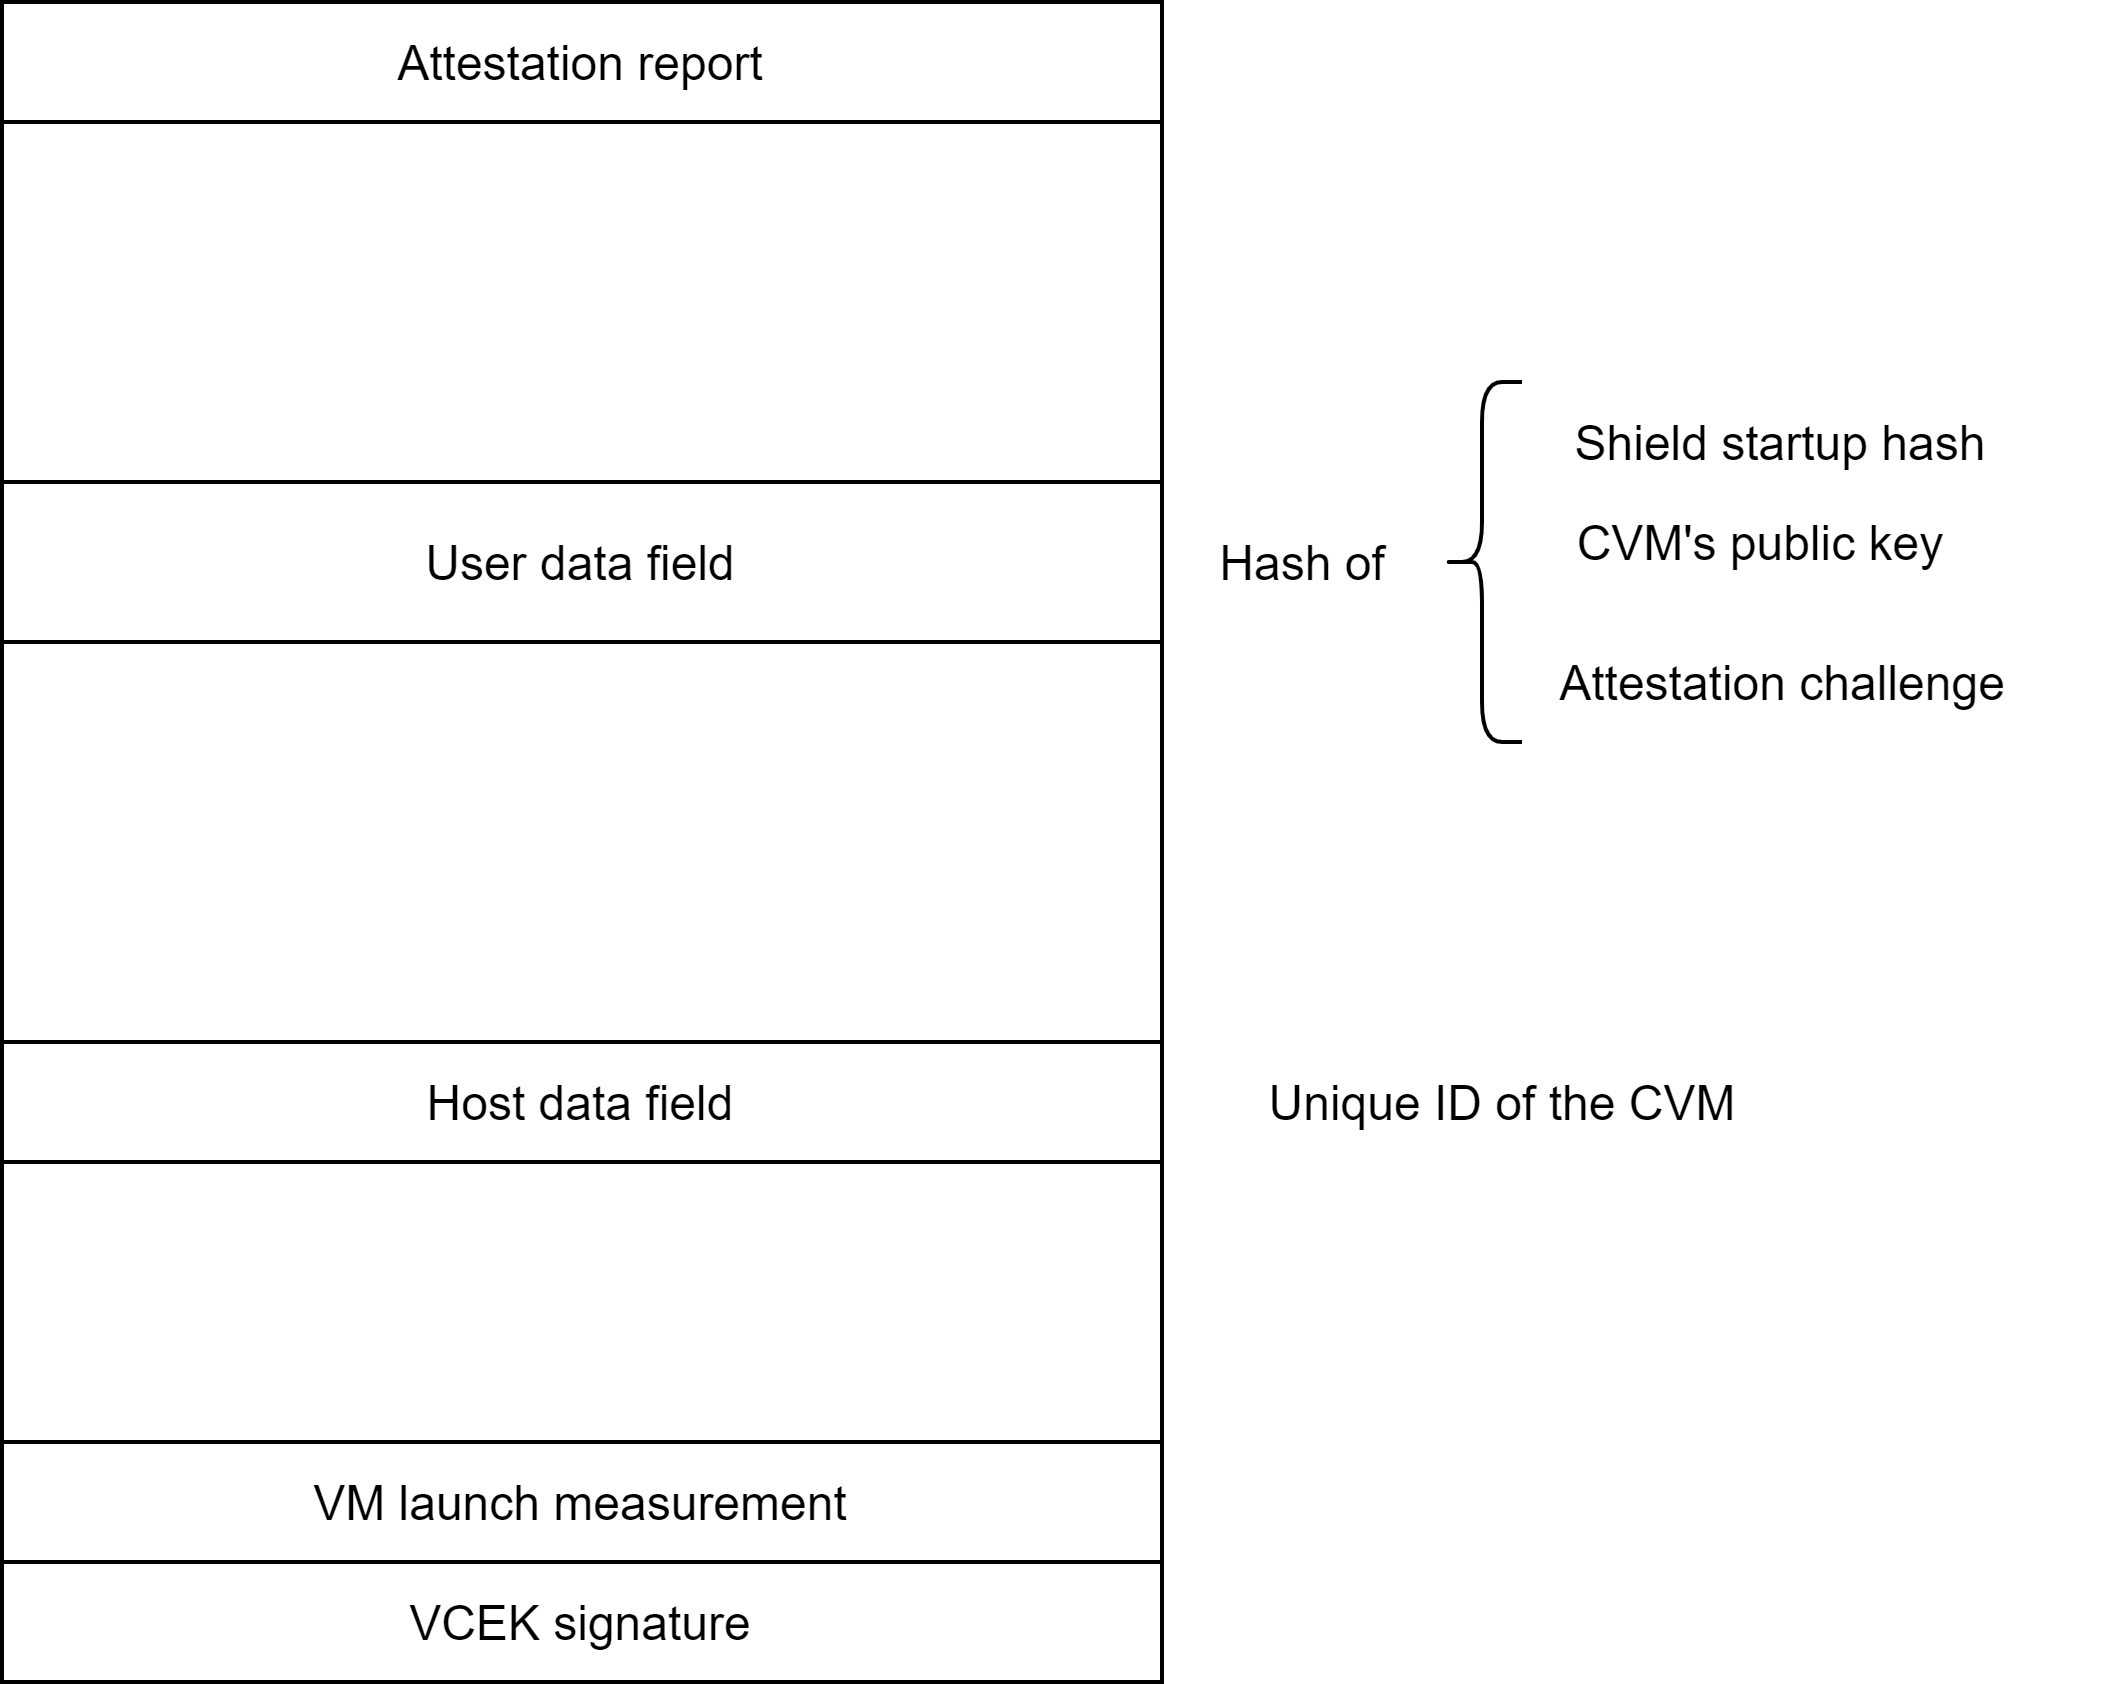
\includegraphics[height=0.3\textheight]{images/attestation_report_format.png}
    \caption[SNP attestation report]{SNP attestation report.}
    \label{fig:attestation_report_format}
\end{figure}
The Secret Manager can verify the report signature using the certificate chain required by AMD KDC~\cite*{snp_kdc}. By checking the measurements of the virtual machine boot process, the Secret Manager can confirm that the enclave is using the correct Qkernel binary because the Qkernel is loaded into the enclave memory by Qvisor using 
SNP\_LAUNCH\_UPDATE~\cite*{snp_firmware}
before VM boot. Notably, the code of the shielding layer is part of the Qkernel binary.

The user-defined data in the report is a hash of the enclave startup measurement and metadata required by the KBS protocol~\cite*{kbs_Attestation_protocol}. These metadata include a RAS public key representing the identity of the enclave and an attestation challenge assigned by the secret manager. An explanation of these metadata can be found in section 3. The enclave startup hash is created by 
the software manager and incorporates all the sensitive data that the enclave loads from the host after the enclave starts. This includes Qkernel command line arguments, binaries, shared libraries, and the public key of the secret manager. By comparing the enclave startup hash to a reference hash provided by the enclave owner, the secret manager can confirm that 
the enclave is configured correctly and that only legitimate binaries are loaded. The secret manager's public key is used for application runtime attestation discussed in Section~\ref{sec:runtime_attesation}.

In order to prevent an attacker from hijacking the secret manager's address and impersonating the secret manager, the KBS attestation protocol~\cite*{kbs_Attestation_protocol} requires that the enclave use the secret manager's public key to authenticate the secret manager during the TLS handshake. Currently, we utilize Kubernetes to mount the public key as a file on the application's rootfs. 
The enclave reads the public key into the guest memory and uses it to set up the TLS connection to the secret manager. When an attacker provides the public key of a fake secret manager to the enclave, the TLS handshake fails due to a mismatch between the public key and the certificate of the real secret manager. In other words, the enclave can only establish a 
connection with the fake secret manager.

The KBS attestation protocol~\cite*{kbs_Attestation_protocol} needs improvement. Since all enclaves use a standard Qkernel binary and applications are created from classic images, the attestation evidence cannot uniquely identify an enclave. Instead, the evidence only certifies that the attester is an enclave running in a TEE with the correctly loaded application. 
When a secret manager manages the secrets of multiple stakeholders, an enclave belonging to one stakeholder could steal the secrets of another. To address this issue, the application owner should assign a unique ID to each enclave. This ID should be added to the host data field of the attestation report by Qvisor during enclave setup. This field is immutable after 
launching the enclave, so the ID is bound to the enclave's attestation evidence. When the secret manager receives an enclave's attestation report, it can use this ID to determine the enclave's identity. In the authentication phase of the KBS attestation protocol, the Secret Manager should bind not only the authentication result but also the enclave's ID to the Cookie identifier. 
This way, the secret manager can map the cookie identifier in the attester's resource request message to its attestation result and the enclave's ID. As such, the secret manager can use the ID and the secret owner's policy to determine whether to grant access to a particular secret to the enclave. The attester's resource request URL should have the following 
format: <repository>/<type>/<tag>, where <repository> is similar to the concept of container image repository, <type> is used to distinguish between different resource types, and <tag> is used to distinguish different versions of a resource. The secret manager should assign each user a unique repository and let them specify which enclaves with IDs can access 
this repository. In this way, we effectively avoid cross-leakage of secrets between different stakeholders.

Note that some of the above features are not implemented. Section~\ref{subsec:Limitations} summarizes the limitations of secure application deployment.

\subsection{Application Runtime Attestation Service}
\label{sec:runtime_attesation}

An application may need to authenticate itself to a remote end at runtime. Quark attestation and provisioning infrastructure enable applications to obtain attestation reports through the guest system call interface. Depending on the application's needs, one of three report formats can be 
obtained: an attestation report generated by the TEE hardware and two software attestation reports created by the shielding layer. The latter contains:

\begin{itemize}
    \item Enclave startup hash.
    \item Enclave ID.
    \item Signature.
    \item Sixty-four bytes of application-specified data.
\end{itemize}

The application can sign the software report with a key issued by the secret manager or by a key it provided. The secret manager's key is sent to the enclave along with the application's secret during the creation of the application process. Software reports offer additional possibilities 
for how the application proves its identity to the remote end. In other words, the remote end can verify the report without the assistance of the hardware provider. Upon verification of the report, the remote end can ensure that the application is as expected by using the enclave startup 
measurement. Besides, application-defined data in a software report is tamper-proof, similar to user data in SNP reports. As previously discussed, the enclave ID guarantees that the remote end can determine the application's identity, which prevents secret cross-leakage. The previous 
section has already discussed the major benefits of enclave startup hash. Additionally, it includes the measurement of the secret manager's public key. Therefore, The remote can be sure that the enclave acquired the secrets from the genuine secret manager during application startup and 
correctly initialized the shielding layer and application. In other words, if the shielding layer is initialized with a compromised policy acquired from a fake secret manager, it can no longer guarantee that the secrets provisioned by the remote won't be compromised




\section{Enclave Runtime Measurement}
\label{sec:Enclave_Runtime_Measurement}
\begin{figure}[!htb]
    \centering
    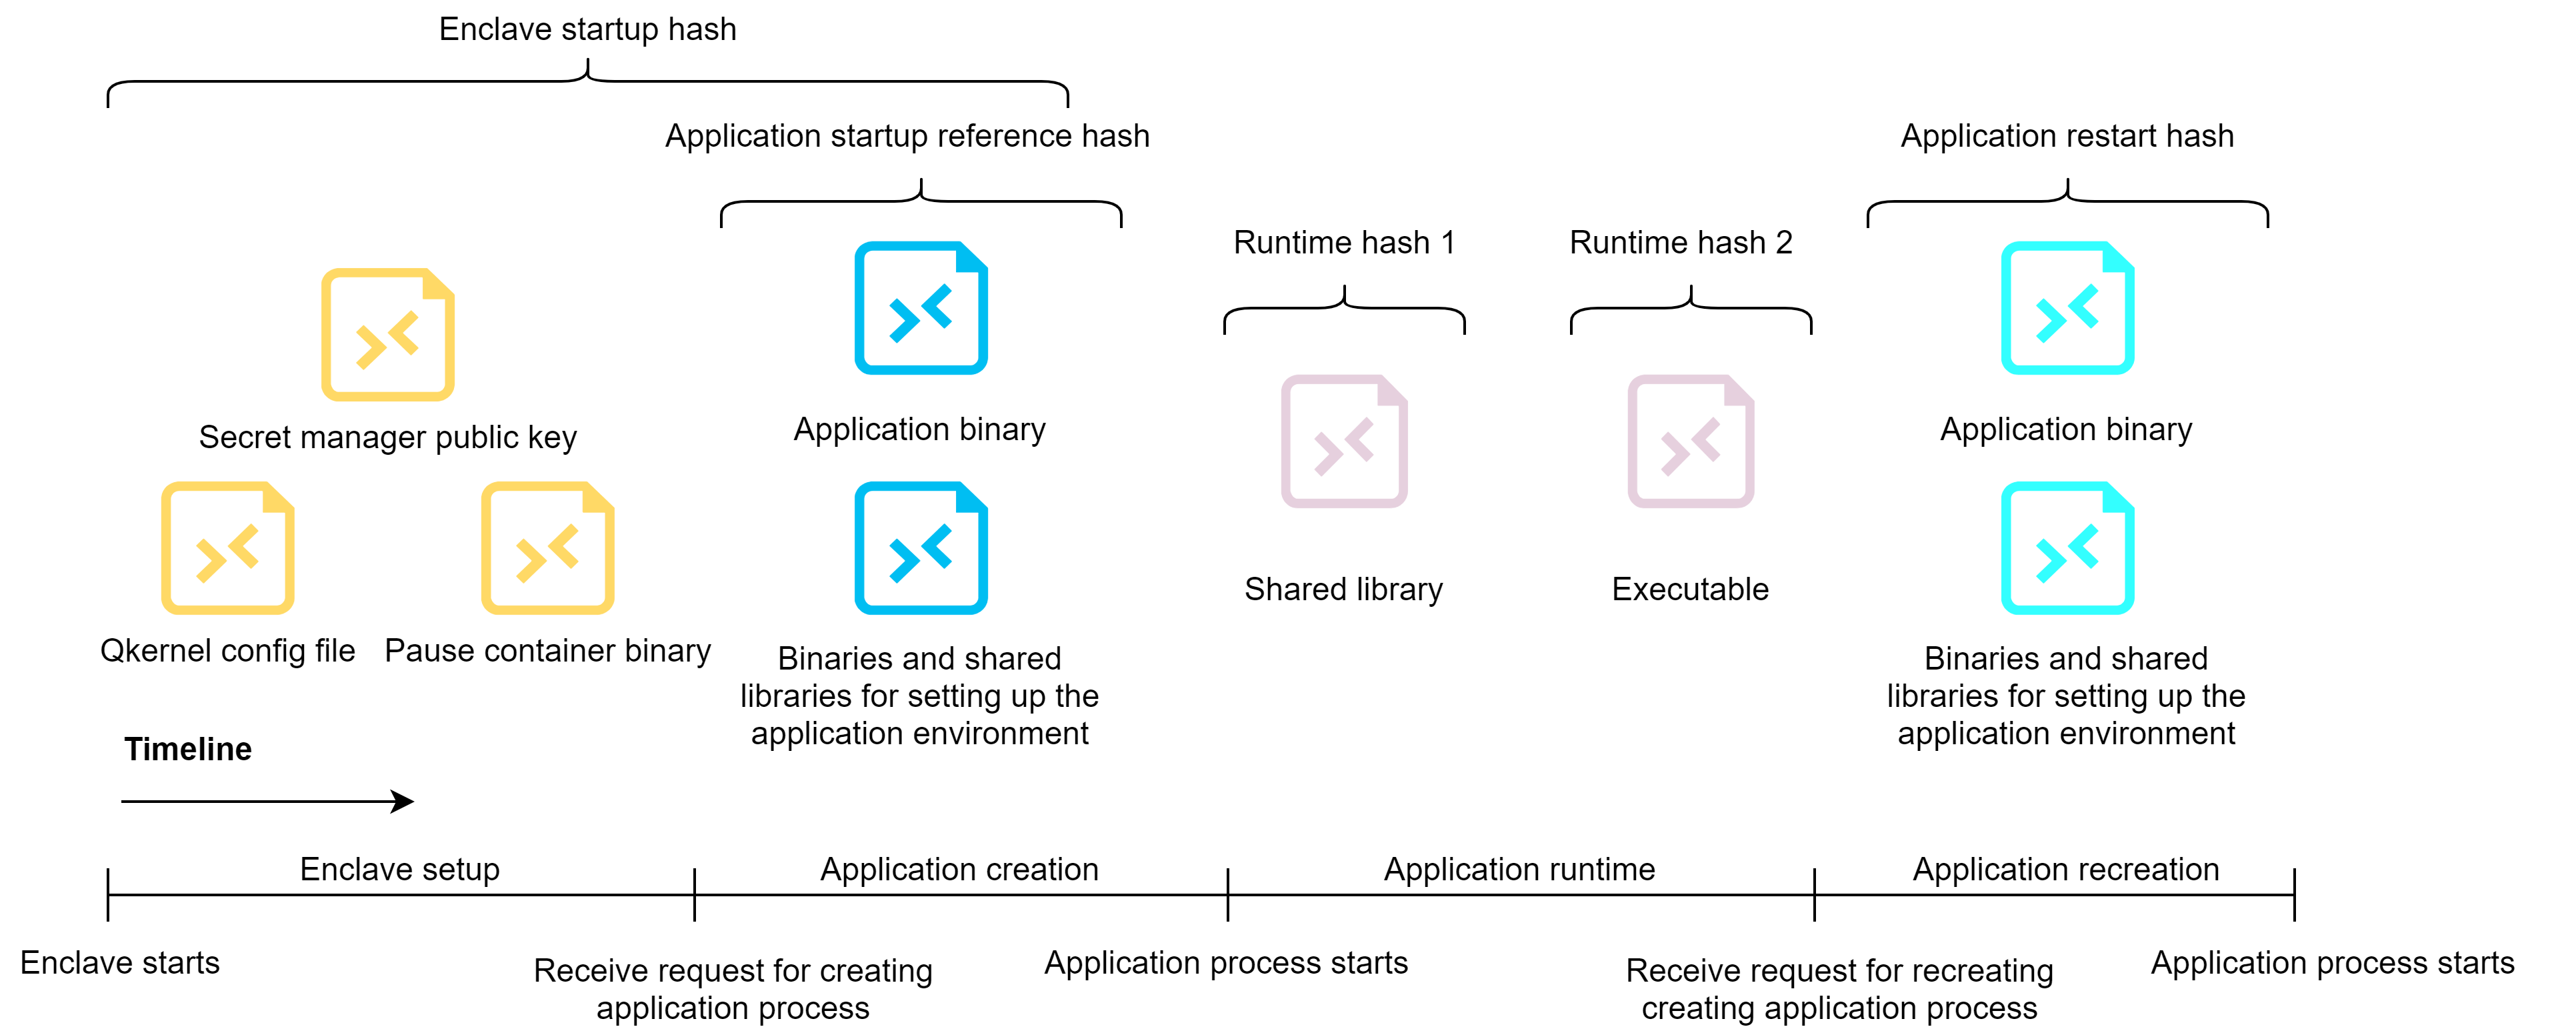
\includegraphics[width=1\textwidth]{images/soft_ware_manager_meausrment.png}
    \caption[Enclave runtime measurement]{Enclave runtime measurement}
    \label{fig:soft_ware_manager_meausrment}
\end{figure}
\todo{fix typo in figure recreating creating}

Enclave runtime measurements are crucial due to the security analysis findings discussed in Chapter~\ref{sec:security_analyse}. However, the AMD SEV SVP does not support enclave runtime measurements~\cite*{snp_firmware}, and the INTEL TDX only allocates four registers for this purpose~\cite*{Intel_tdx_whitepaper}. Consequently, we provide a software measurement 
manager in the shielding layer to measure the data loaded from the host while the enclave is running. As shown in Figure~\ref{fig:soft_ware_manager_meausrment}., The software measurement manager provides the following important hashes:

Enclave startup hash. This value refers to the measures of host-loaded data until the application process starts. This includes the secret manager's key, the Qkernel's configuration file, the application's binary, and the multiple binaries and shared libraries loaded to set up the application environment. Additionally, since each Pod starts a pause container 
first upon startup, the enclave startup hash also contains a measurement of the binaries and shared libraries that were loaded when the pause container was created. The attestation and provisioning agent include this hash in the attestation report, which is conveyed to the secret manager. The secret manager compares the measurement to the reference value provided 
by the enclave owner to ensure the enclave is properly configured. This hash effectively solves the problems 1,2,3 identified in Chapter 3.
\todo{add link}

Application startup reference hash. As shown in the figure, this value records the measure of all binaries and shared libraries during the application's first startup. This measurement is a subset of the enclave's startup measurements and is stored in the enclave's memory. It will be used as a reference value for the application restart hash to ensure the 
integrity of the binary and shared libraries load during the restart. 

Runtime hash. The runtime hash represents a measurement of an executable or shared library loaded in the application runtime. Unlike the enclave startup hash, which is forwarded to the secret manager, the runtime hash is verified by the software manager. The shielding layer's policy holds reference hashes, as shown in Figure~\ref{fig:measurement}. In this case, 
the software measurement manager measures a binary and compares the result with the reference value from the policy. If the two values differ, the enclave will panic. This ensures the correct shared library or executable is loaded during application runtime.
\begin{figure}[!htb]
    \centering
    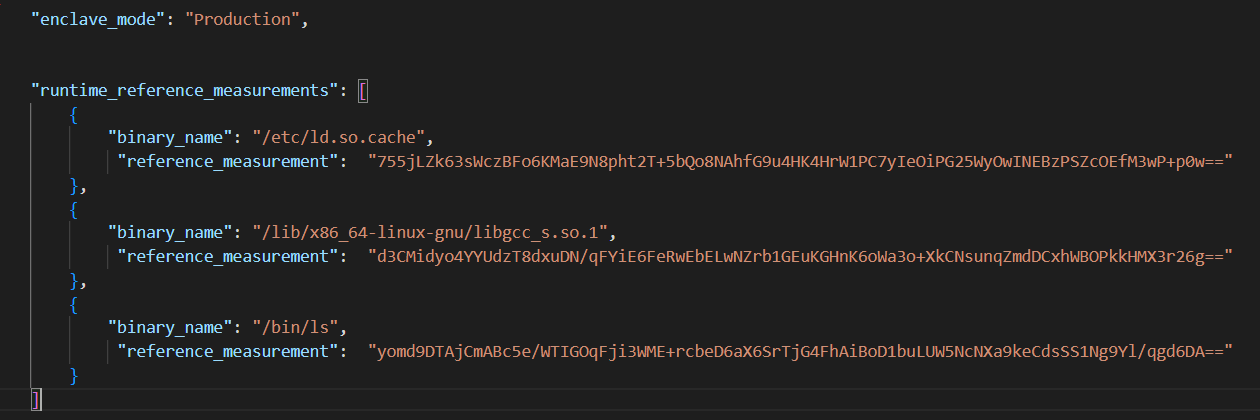
\includegraphics[width=0.8\textwidth]{images/measurement.png}
    \caption[Reference value in shielding layer's policy for runtime hashes]{Reference value in shielding layer's policy for runtime hashes}
    \label{fig:measurement}
\end{figure}

Application restart hash. When the application crashes and restarts, the software measurement manager measures the binaries and shared libraries. The resulting application restart hash will be compared with the application startup reference hash before launching the application process. If the two do not match, the Enclave panics. In this way, the enclave 
ensures that the host data loaded at restart is the same as the data from the first application startup. The application startup reference hash is a subset of the enclave's startup hash, checked by the secret manager. Thus comparing the two hashes ensures the integrity of the binaries and shared libraries loaded at application restart. 

Regarding obtaining the reference values for enclave startup hash and runtime hashes, we implemented an enclave mode called Development. When running in this mode, the enclave will print these hashes to the Qkernel log on the host. The enclave owner should run the enclave in a trusted environment to obtain these reference values.

\section{New Pattern for EXEC Requests}
\label{sec:design_EXEC_Requests}
\begin{figure}[!htb]
    \centering
    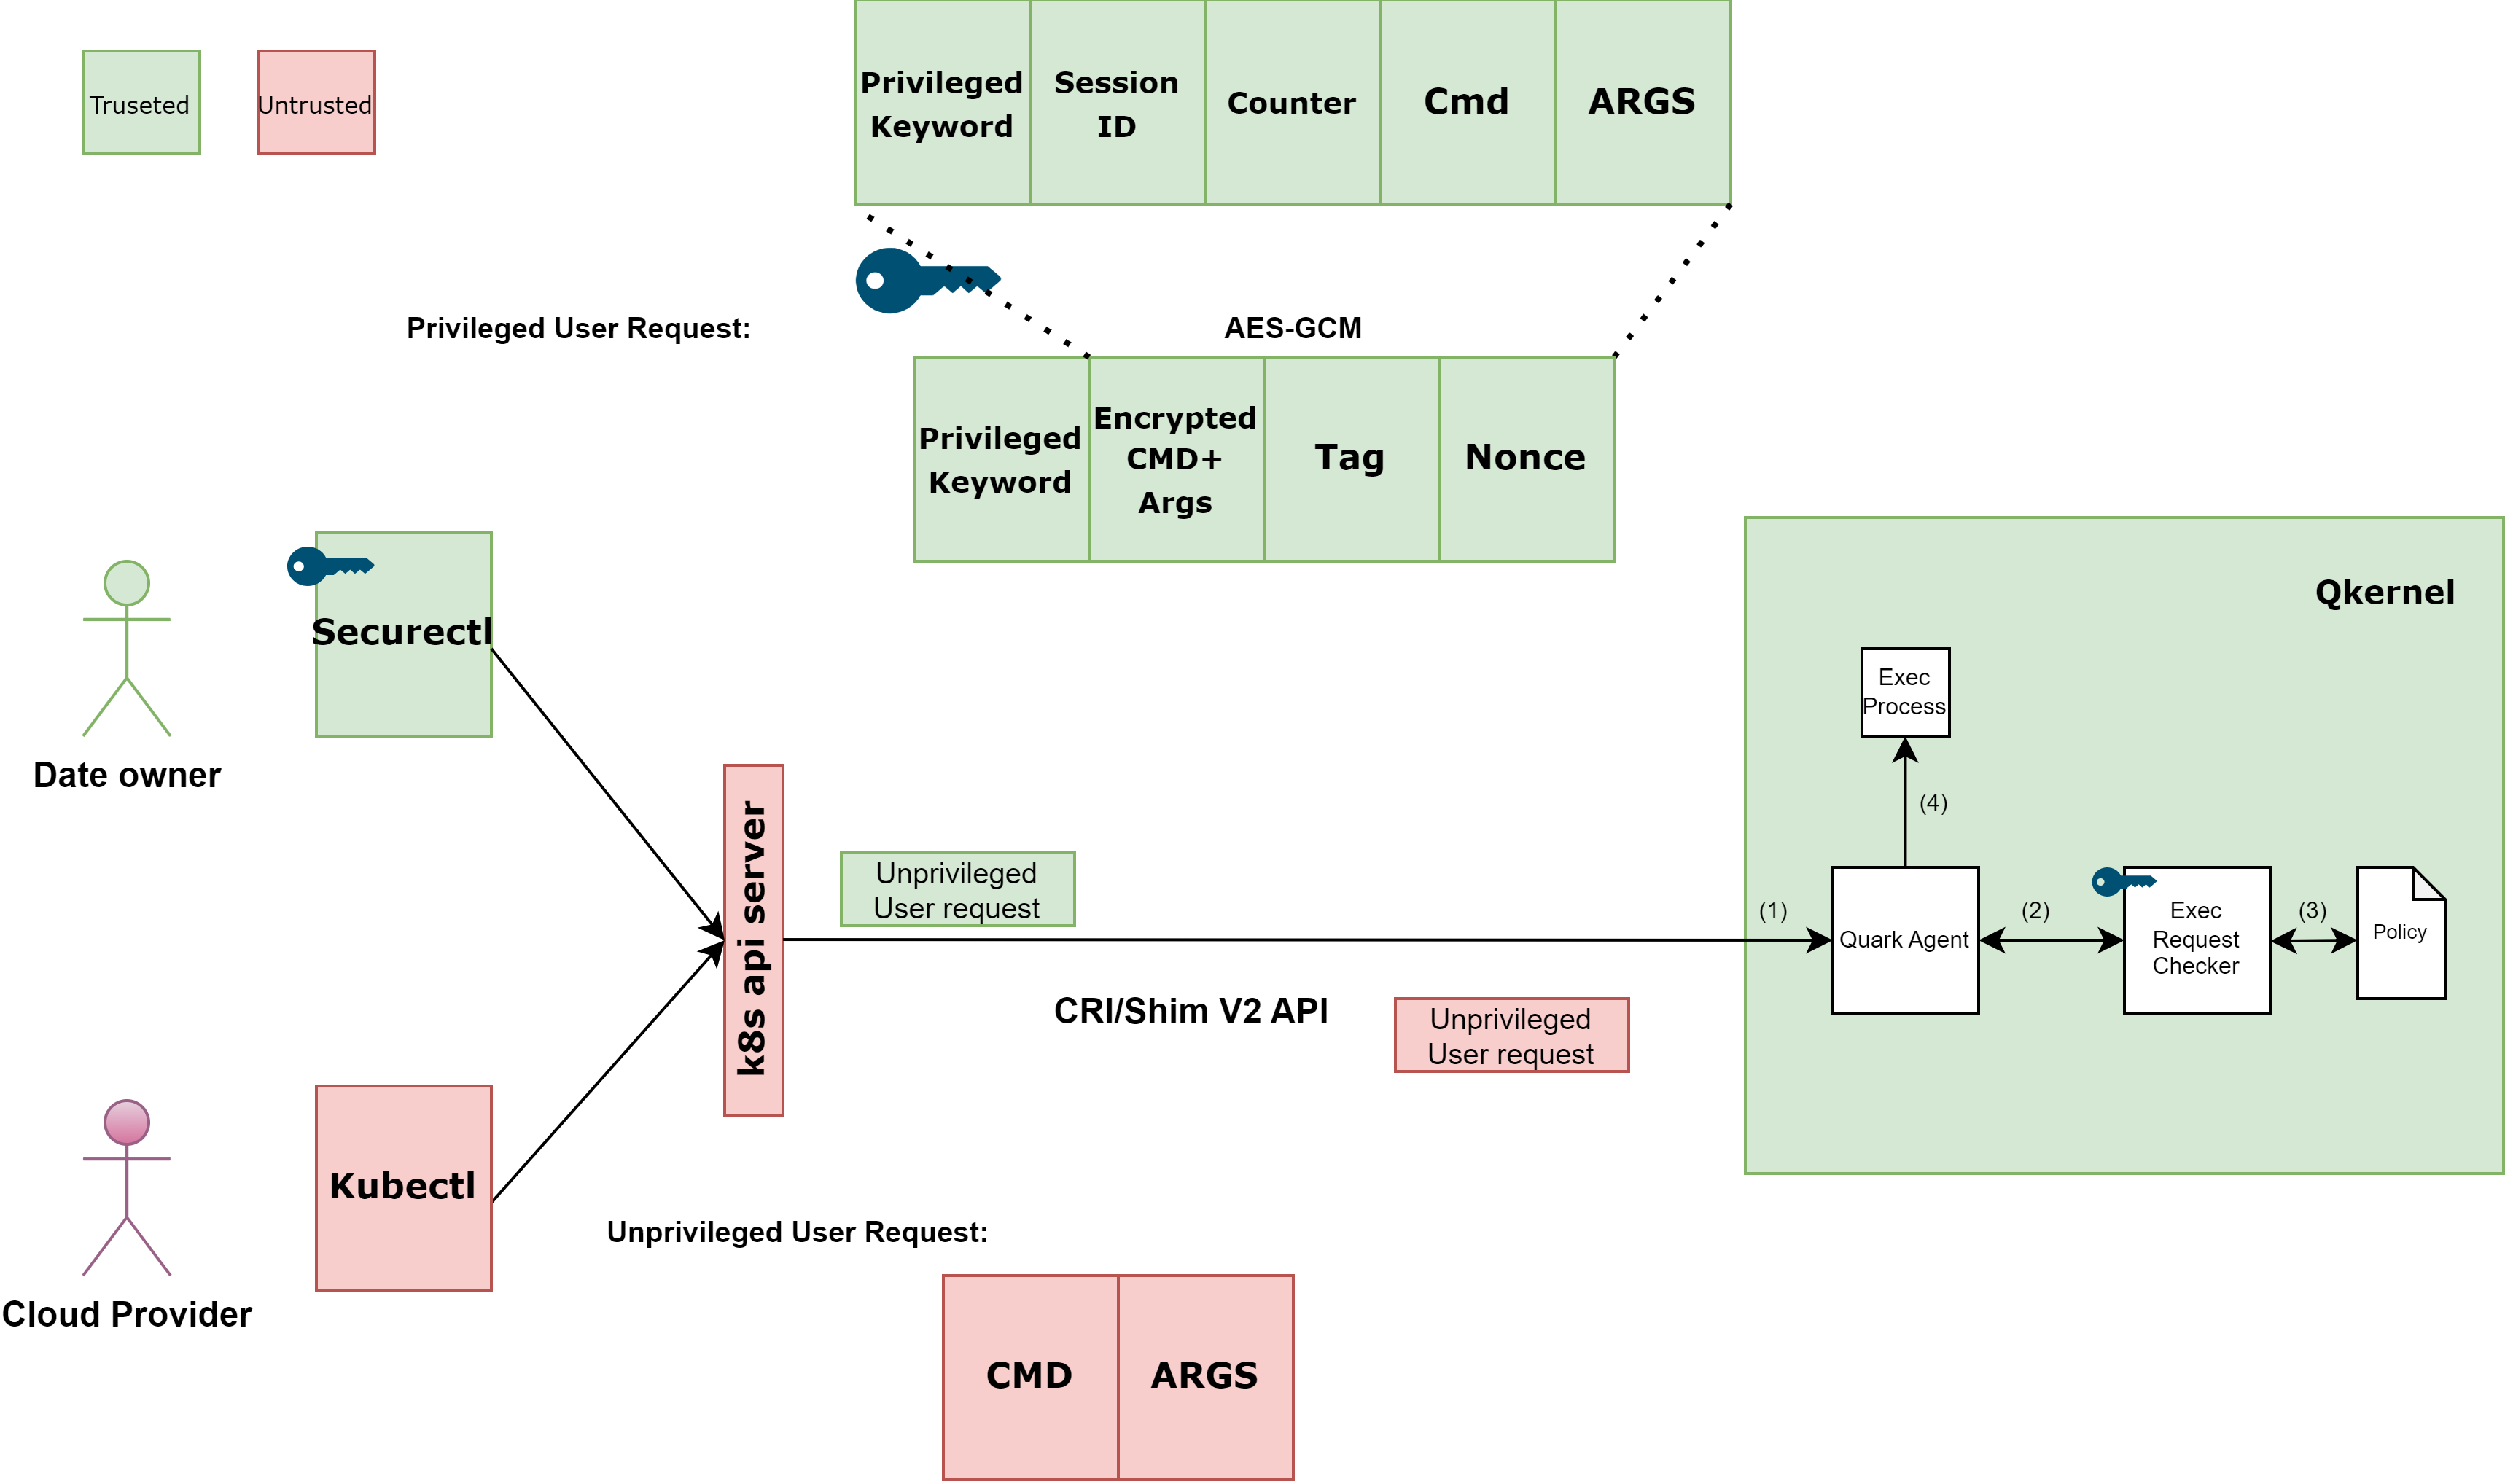
\includegraphics[width=0.8\textwidth]{images/new_pattern_of_exec.png}
    \caption[New Pattern for EXEC Requests]{New Pattern for EXEC Requests}
    \label{fig:new_pattern_of_exec}
\end{figure}

We propose a new pattern for EXEC requests to address issues \todo{add ref} and \todo{add ref} identified in the security analysis. As illustrated in Figure~\ref{fig:new_pattern_of_exec}, The design divides EXEC requests into two categories, namely privileged and unprivileged EXEC requests. Privileged EXEC requests are issued by privileged users 
(i.e., enclave owners), while untrusted entities issue unprivileged requests. An untrusted entity here refers to someone other than the enclave owner. Privileged and non-privileged users send privileged or non-privileged requests to the enclave using securectl or kubectl, respectively. Both requests
are redirected to the enclave through the Kubernetes. Upon receiving an EXEC request, the Quark agent forwards it to the Exec request checker. According to the enclave policy, the Exec request checker will authenticate and access control the request. The Quark agent will decide whether to create the 
EXEC process based on the result returned by the EXEC request checker.






\begin{figure}[!htb] 
    \begin{subfigure}[b]{0.3\linewidth}
      \centering
      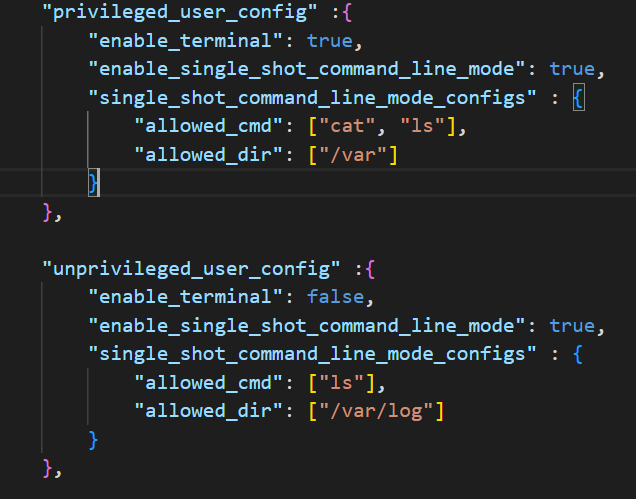
\includegraphics[width=0.9\linewidth]{images/exec_policy.png} 
      \caption{Policy for EXEC requests} 
      \label{fig:exec_policy} 
      \vspace{4ex}
    \end{subfigure}%% 
    \begin{subfigure}[b]{0.6\linewidth}
      \centering
      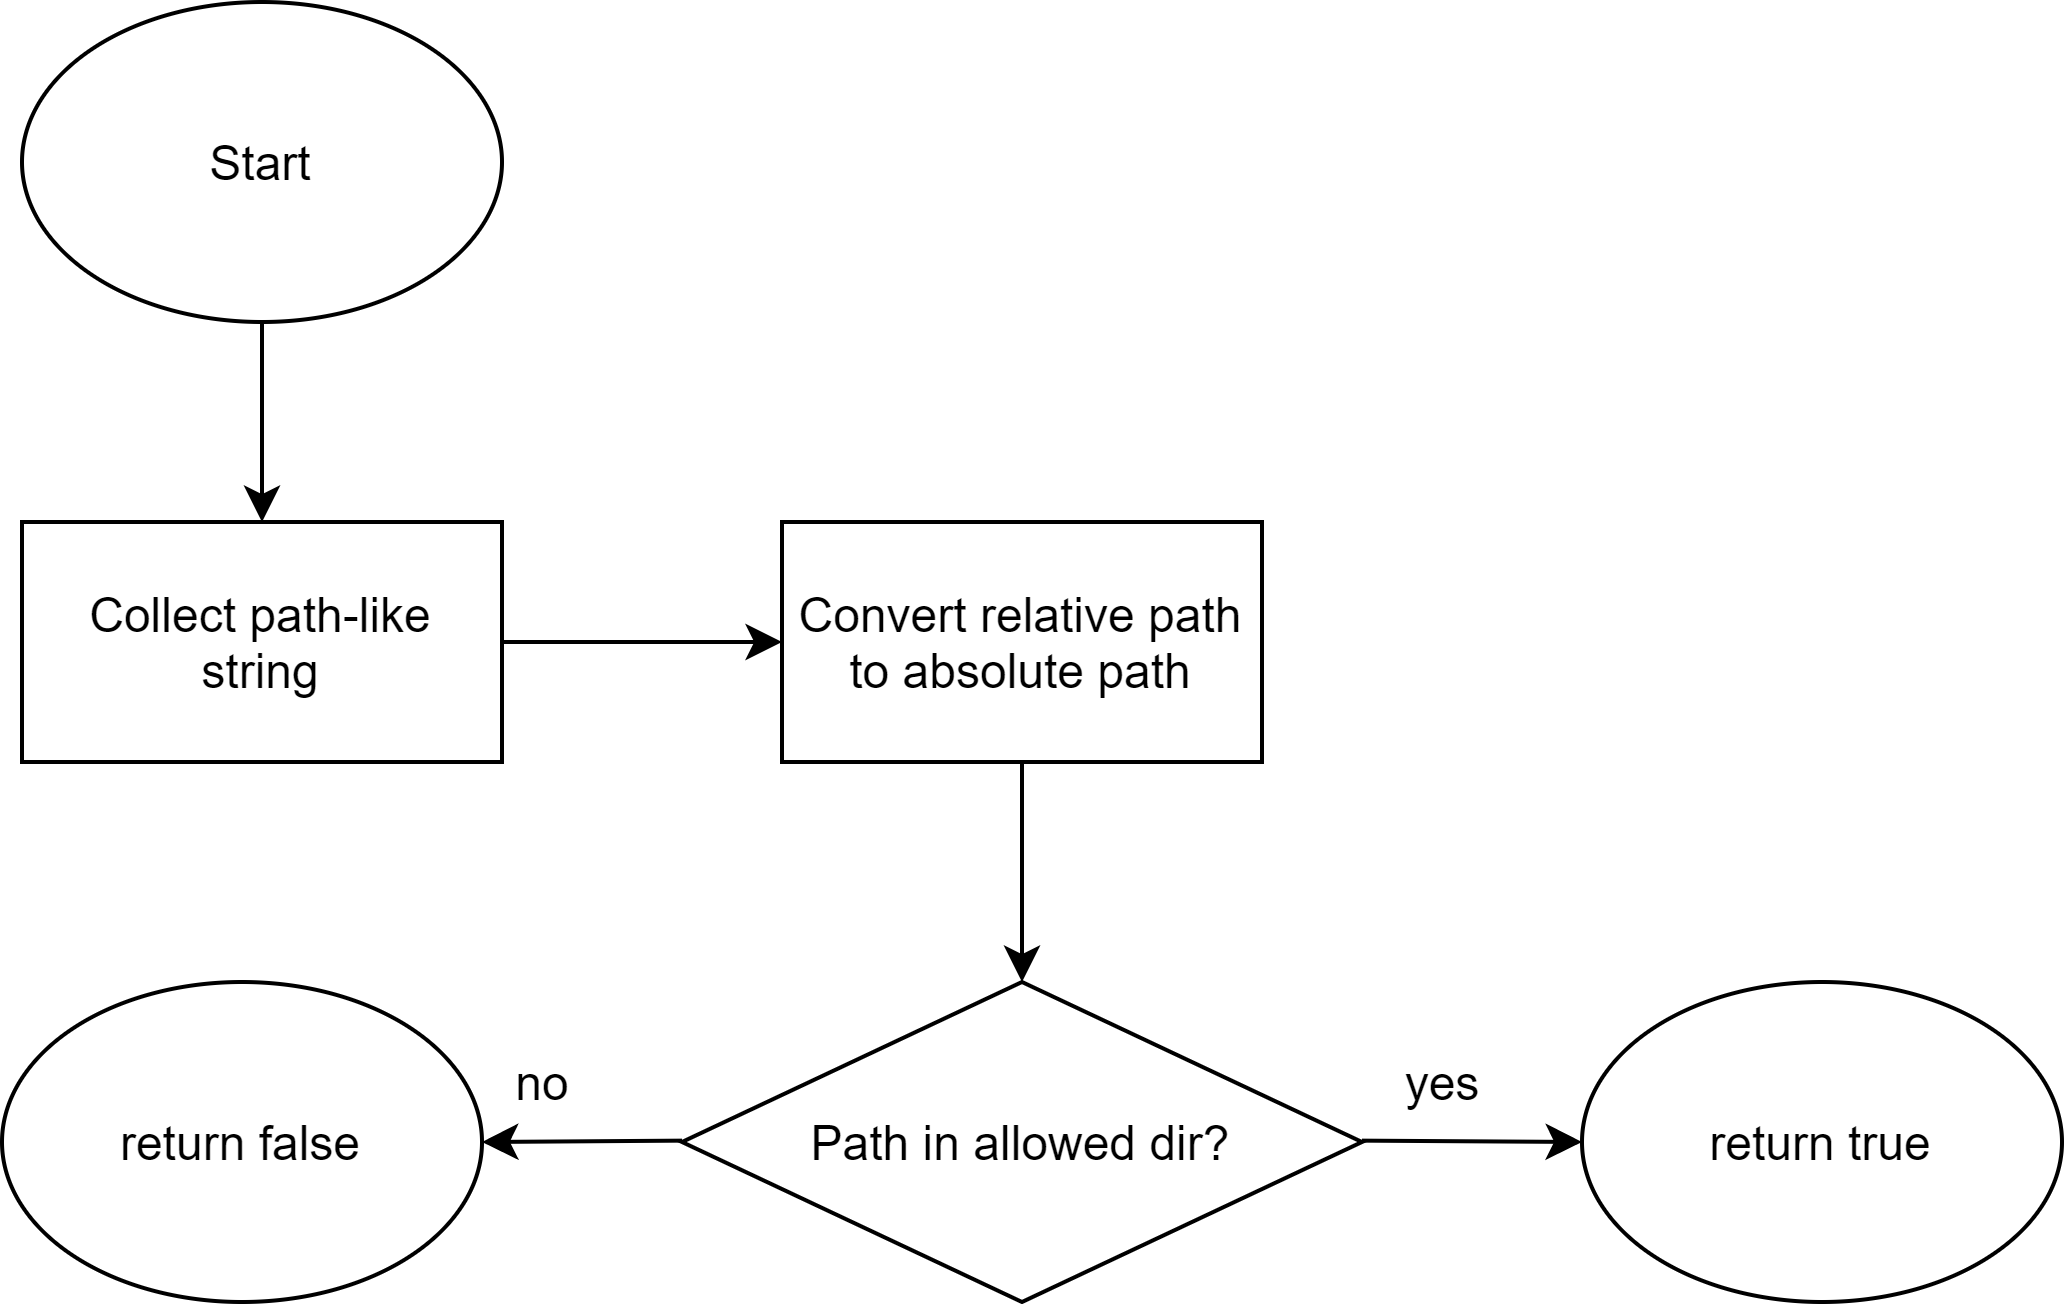
\includegraphics[width=0.9\linewidth]{images/algo_for_path_checking.png} 
      \caption{Algorithm for validating command parameters against directory whitelist} 
      \label{fig:algo_for_path_checking} 
      \vspace{4ex}
    \end{subfigure} 
    \caption{Policy for EXEC requests and algorithm for validating command parameters}
    \label{fig3} 
\end{figure}


The policy used by the exec request checker is in Figure~\ref{fig:exec_policy}. This policy is part of the enclave policy. Each user level possesses an allowlist of commands, "allowed\_cmd," and an allowlist of directories, "allowed\_dir." The command allowlist specifies what commands the user can issue, while the 
directory allows list controls which directories a command can access. When an EXEC request is received, the EXEC checker examines all path-like strings in the command argument and verifies if they exist in the directory allowlist. The EXEC checker also checks whether the current working directory of 
a no-arguments command is a subpath of a directory in the directory allowlist so that the command can only be executed in some specific directories. Notably,  directory whitelisting does not apply to terminal allocation commands like /bin/sh, /bin/bash, and sh. This permits users to allocate a terminal 
from any directory. For instance, this policy enables privileged users to issue cat, ls, and /bin/sh commands. The cat and ls commands are restricted to the /var directory and its subdirectories. Therefore, any attempt to execute commands in other directories (e.g., cat / and cat /bin) will be denied. 
On the other hand, since /bin/sh is included in the command allowlist, privileged users can allocate a terminal. Moreover, if a privilege level's command whitelist is empty, all commands issued by the user with this privilege level will be rejected.



The EXEC checker employs the algorithm presented in~\ref{fig:algo_for_path_checking} to validate the command parameters. It is important to note that the command and its arguments are conveyed as an array of strings from the user to the enclave. The first element of the array represents the command, and the subsequent elements 
correspond to the command's arguments. Consequently, the algorithm iterates through this array to inspect all the command's arguments, capturing absolute and relative paths. Absolute paths encompass strings beginning with '/,' whereas relative paths are the strings containing '.'' or '/.' Following 
this, the algorithm utilizes the command's current working directory to convert relative paths into absolute paths. Finally, it checks all paths against the directory allowlist. It returns false if a path is not a subpath defined in the policy.


\subsection{Protection for Privileged Exec Request}
\label{sec:design_prptect_privileged_request}
\begin{figure}[!htb]
    \centering
    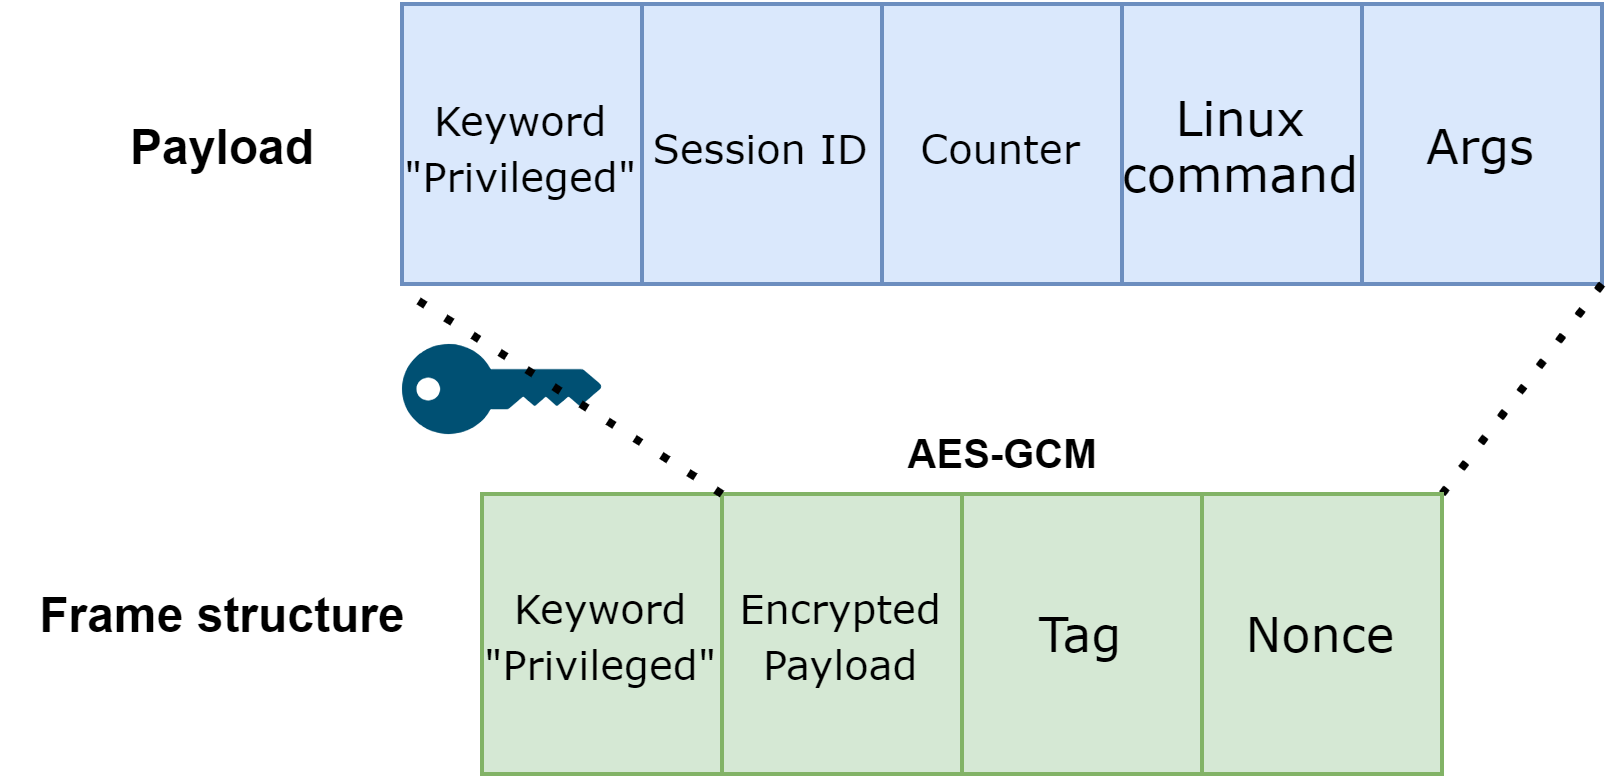
\includegraphics[width=0.4\textwidth]{images/exec_frame.png}
    \caption[Frame structure  for protecting privileged exec request]{Frame structure  for protecting privileged exec request}
    \label{fig:exec_frame}
\end{figure}
The frame structure shown in Figure~\ref{fig:new_pattern_of_exec} protects privileged commands and distinguishes them from non-privileged commands. The frame structure encapsulates the string "Privileged," the AES-GCM encrypted payload, the AES-GCM~\cite*{aes_gcm} random number (nonce) used for payload decryption, and the authentication tag. 
The plaintext payload contains the keyword "Privileged," the session ID, a counter,  the Linux command, and its parameters. K8S and the Open Container Initiative require that commands and their parameters in EXEC requests be passed as a vector of strings. For example, ["cat", "/var/log"]~\cite*{k8s}. As such, 
the encrypted payload, nonce, and tag in the frame structure are encoded in base64, and the frame is passed as a string array to the enclave via the Kubernetes API. Note that the string array is part of the EXEC request process specification called args (See section\todo{add ref}). Upon receiving an EXEC request, 
the EXEC request checker can determine if the request is privileged by viewing the first element of the arg array. If the element is the keyword Privileged", the request will be classified as privileged.

AES-GCM~\cite*{aes_gcm} ensures the confidentiality, authenticity, and integrity of privileged commands and their arguments. Besides, it is easy to deploy, requiring only a shared key. After a successful remote attestation, a key is shared between the application owner and the enclave. The application owner can 
use this key to encrypt privileged commands and their parameters. When the enclave receives a privileged request, the exec request checker can use the key to confirm that the request was generated by a privileged user who knows the key (authentication), verify the request's integrity, and decrypt the 
request.


The monotonic counter and session are designed to prevent reply attacks. The counter is assigned by the enclave to a privileged user. When the value of the monotonic counter in an EXEC request is smaller than the reference value stored in the enclave, the request will be rejected. Since there may be 
more than one privileged user, it is hard to share the counter. Therefore, we introduce sessions. In this case, the enclave will assign each privileged user a random session id and a unique counter. This id and counter are stored in the enclave and will be sent to a privileged user via a secure channel. 
The privileged user can use the session id and counter to construct a privileged EXEC request. Note that the counter is added by one after each EXEC request. With the session and counter, we avoid the following two reply attacks. First, the attacker sends a request that belongs to an illegal session, 
i.e., the enclave does not store the session id. Second, the attacker has sent an outdated request to the enclave. This means that the counter value in a request is less than the current counter value recorded in the enclave for the requested session ID. In this case, the enclave will refuse to 
execute it.
\subsection{Session Assignment and Policy Updates}
\label{subsec:design_policy_session_update}
\begin{figure}[!htb]
    \centering
    
    \begin{minipage}{0.9\textwidth}
    \begin{subcolumns}[0.62\textwidth]
      \subfloat[Workflow of session assignment\label{fig:session_base_auth}]{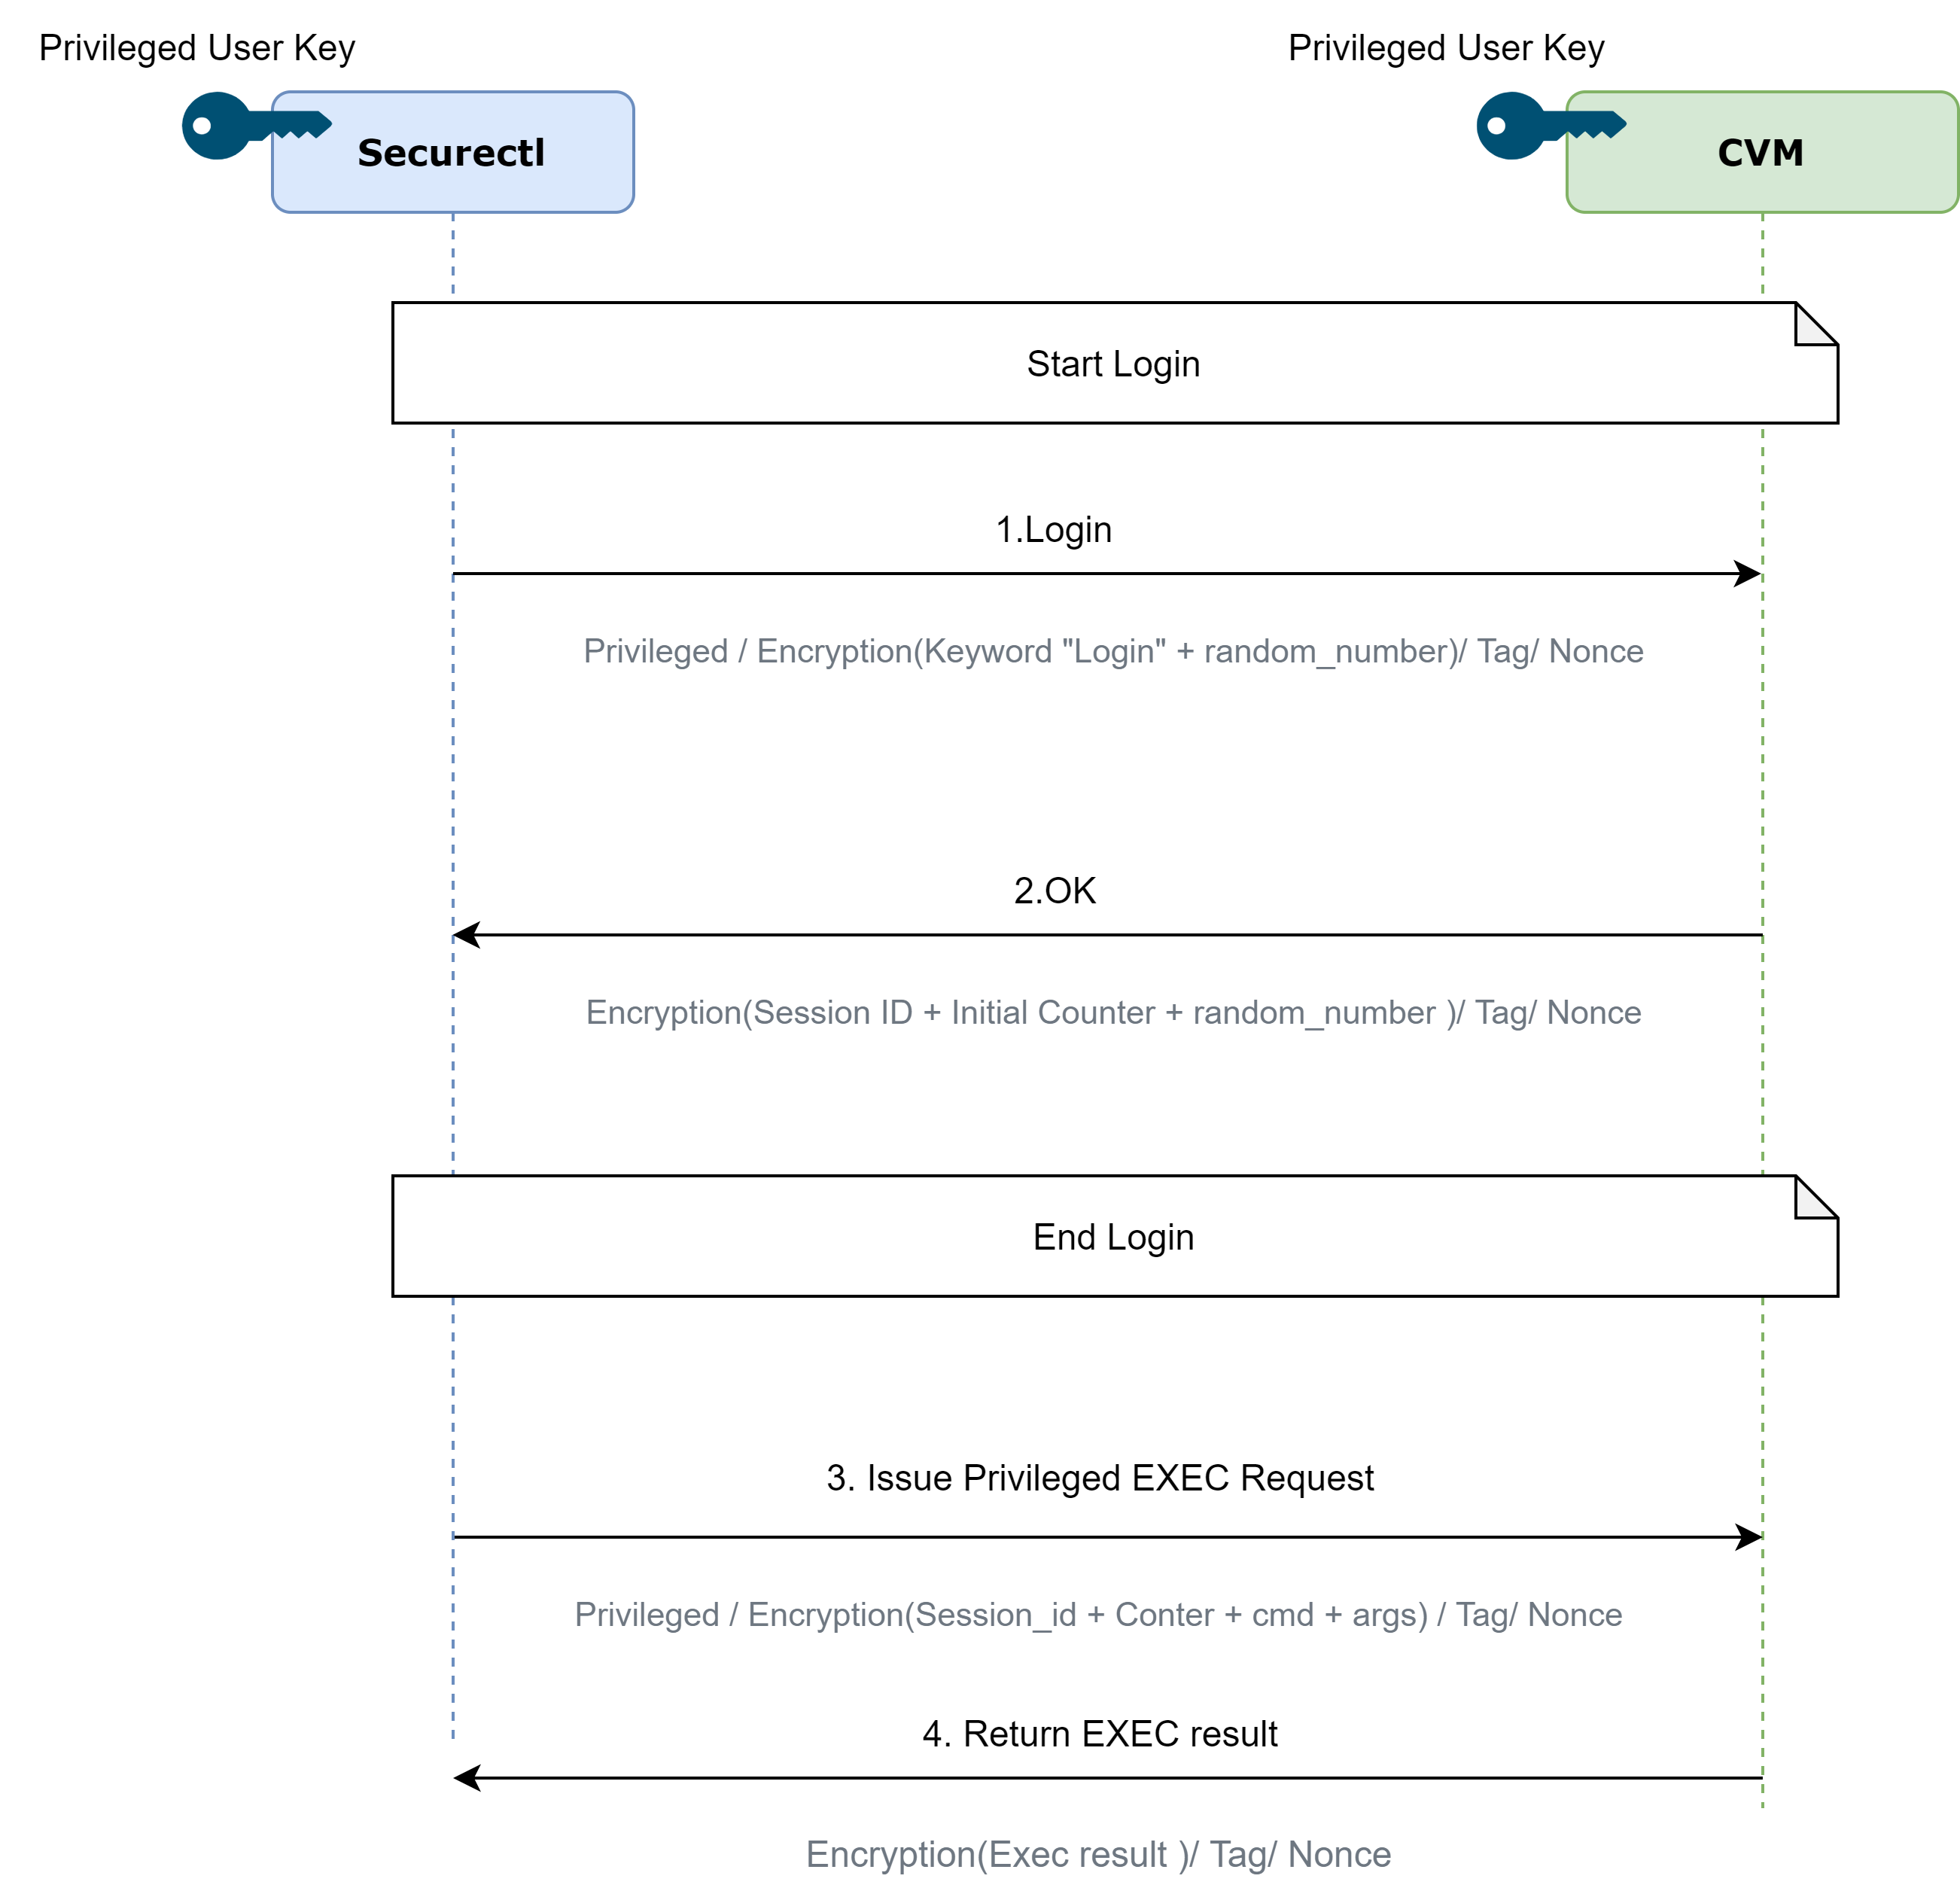
\includegraphics[width=\subcolumnwidth]{images/session_base_auth.PNG}}

    \nextsubcolumn[0.33\textwidth]
      \subfloat[Frame structure  for session allocation\label{fig:session_allocation}]{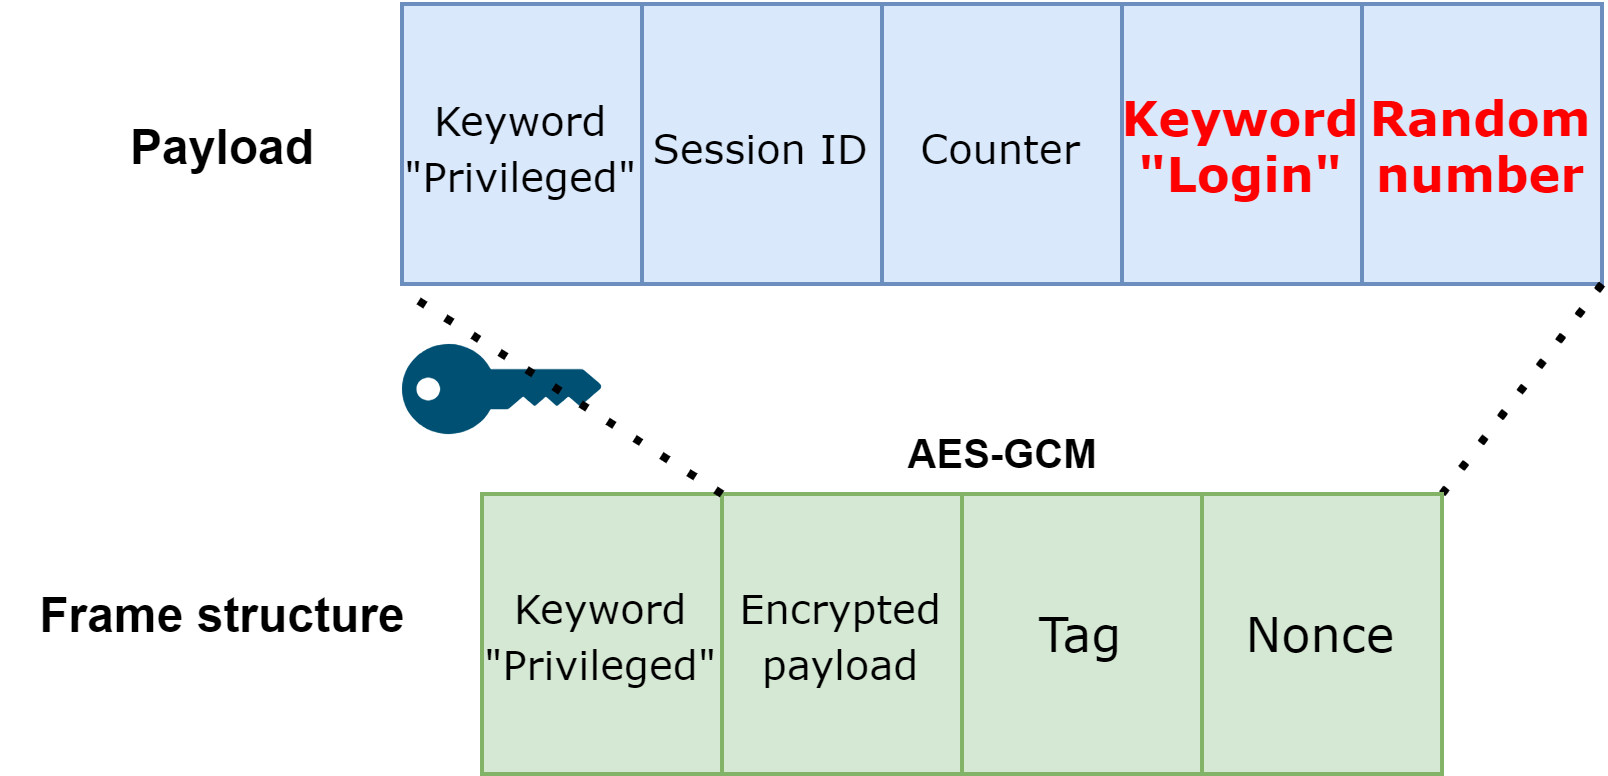
\includegraphics[width=\subcolumnwidth]{images/session_allocation.PNG}}

    \nextsubfigure
      \subfloat[Frame structure  for policy updates\label{fig:policy_frame}]{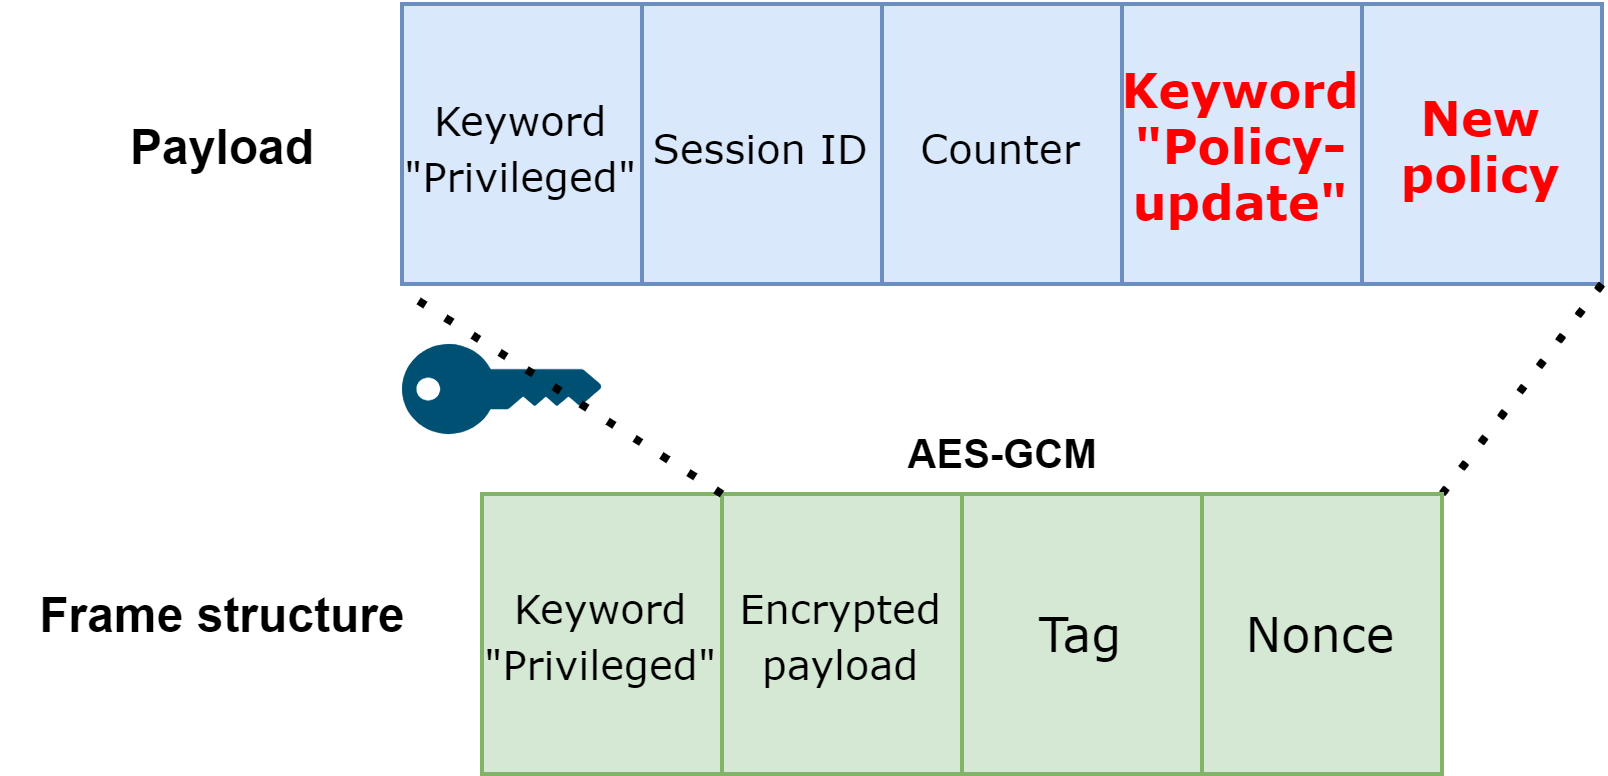
\includegraphics[width=\subcolumnwidth]{images/policy_frame.PNG}}
    \end{subcolumns}
    \end{minipage}
    
    \caption[Session Assignment and Policy Updates]{Session Assignment and Policy Updates}
    \label{fig:session_policy}
\end{figure}


Figure~\ref{fig:session_base_auth} demonstrates how a privileged user gets a session. The privileged user submits a login request using securectl in the login phase. The login request is a privileged EXEC request with the format visualized in Figure~\ref{fig:session_allocation}. Instead of a real Linux command, the keyword Login and a random number 
are used as the command and parameter. The random number is used to prevent reply attacks. After the enclave verifies and decrypts the encrypted payload, it checks the command in the payload. If the command is the keyword Login, it assigns a session ID and a unique counter to the privileged user. 
These two values are stored in the enclave and returned to securectl securely. Specifically, it creates a process when that EXEC request is received. However, the keyword "Login" is not a Linux command. Thus, the enclave replaces the command executed by the exec process with" ls." Once the process 
completes running ls and writes the result to its STDOUT, the STDIO shield will intercept the data and replaces it with the session ID and counter. Since the login request is privileged, the STDIO shield will encrypt the data before sending it to the user. 

When the keyword "enabale\_policy" is true in the enclave policy, privileged users can use securectl to update the enclave policy. Similar to the session allocation request, the policy is updated by sending a privilege-level command to the enclave. The format of the command can be found in~\ref{fig:policy_frame}. Unlike 
the session request's payload, it uses the keyword policy-update as the command, with the new enclave policy as the command's argument

\section{Guest User Space Process STDIO Protection}
\label{sec:design_STDIO_PROTECTION}
We propose a guest user-space process STDIO Shield to tackle the identified security issues (~\ref{vulnerabilities:2}, ~\ref{vulnerabilities:3}, ~\ref{vulnerabilities:6}). In the following, We explain how the STDIO Shield protects both non-interactive and interactive processes. It is important to note that privileged processes refer to both the application process and processes executing privileged EXEC commands. The distinction between interactive and non-interactive processes lies in their STDIO, specifically whether it is of terminal type. 


\subsection{Distinguish the STDIO type of the processes}

The guest user space can accommodate various types of processes, including privileged-level non-interactive EXEC processes, privileged-level interactive EXEC processes, session or policy update processes, and various non-privileged-level EXEC processes. The STDIO shield handles the STDIO of these processes differently. For instance, 
to send the session id to a user, the shield intercepts the session process's STDOUT, replaces the content with the session ID assigned to the user, and encrypts it to maintain confidentiality. Similarly, data written to the STDOUT and STDERR of privileged-level non-interactive processes is encrypted. Conversely, data belonging 
to non-privileged level process STDIO remains unaltered. Consequently, the STDIO shield necessitates a mechanism for discerning between the various types of process STDIO.
 
The file descriptor representing the STDIO of a process cannot be used to distinguish between different processes' STDIO streams, as the file descriptors for STDIN, STDOUT, and STDERR are fixed as 0, 1, and 2, respectively. Qkernel, however, implements a virtual file system. Like the Linux kernel, each file descriptor in the Qkernel filesystem corresponds to 
a unique inode with a unique id. Therefore, the inode id can differentiate between the STDIO streams of different processes.
\begin{figure}[!htb]
    \centering
    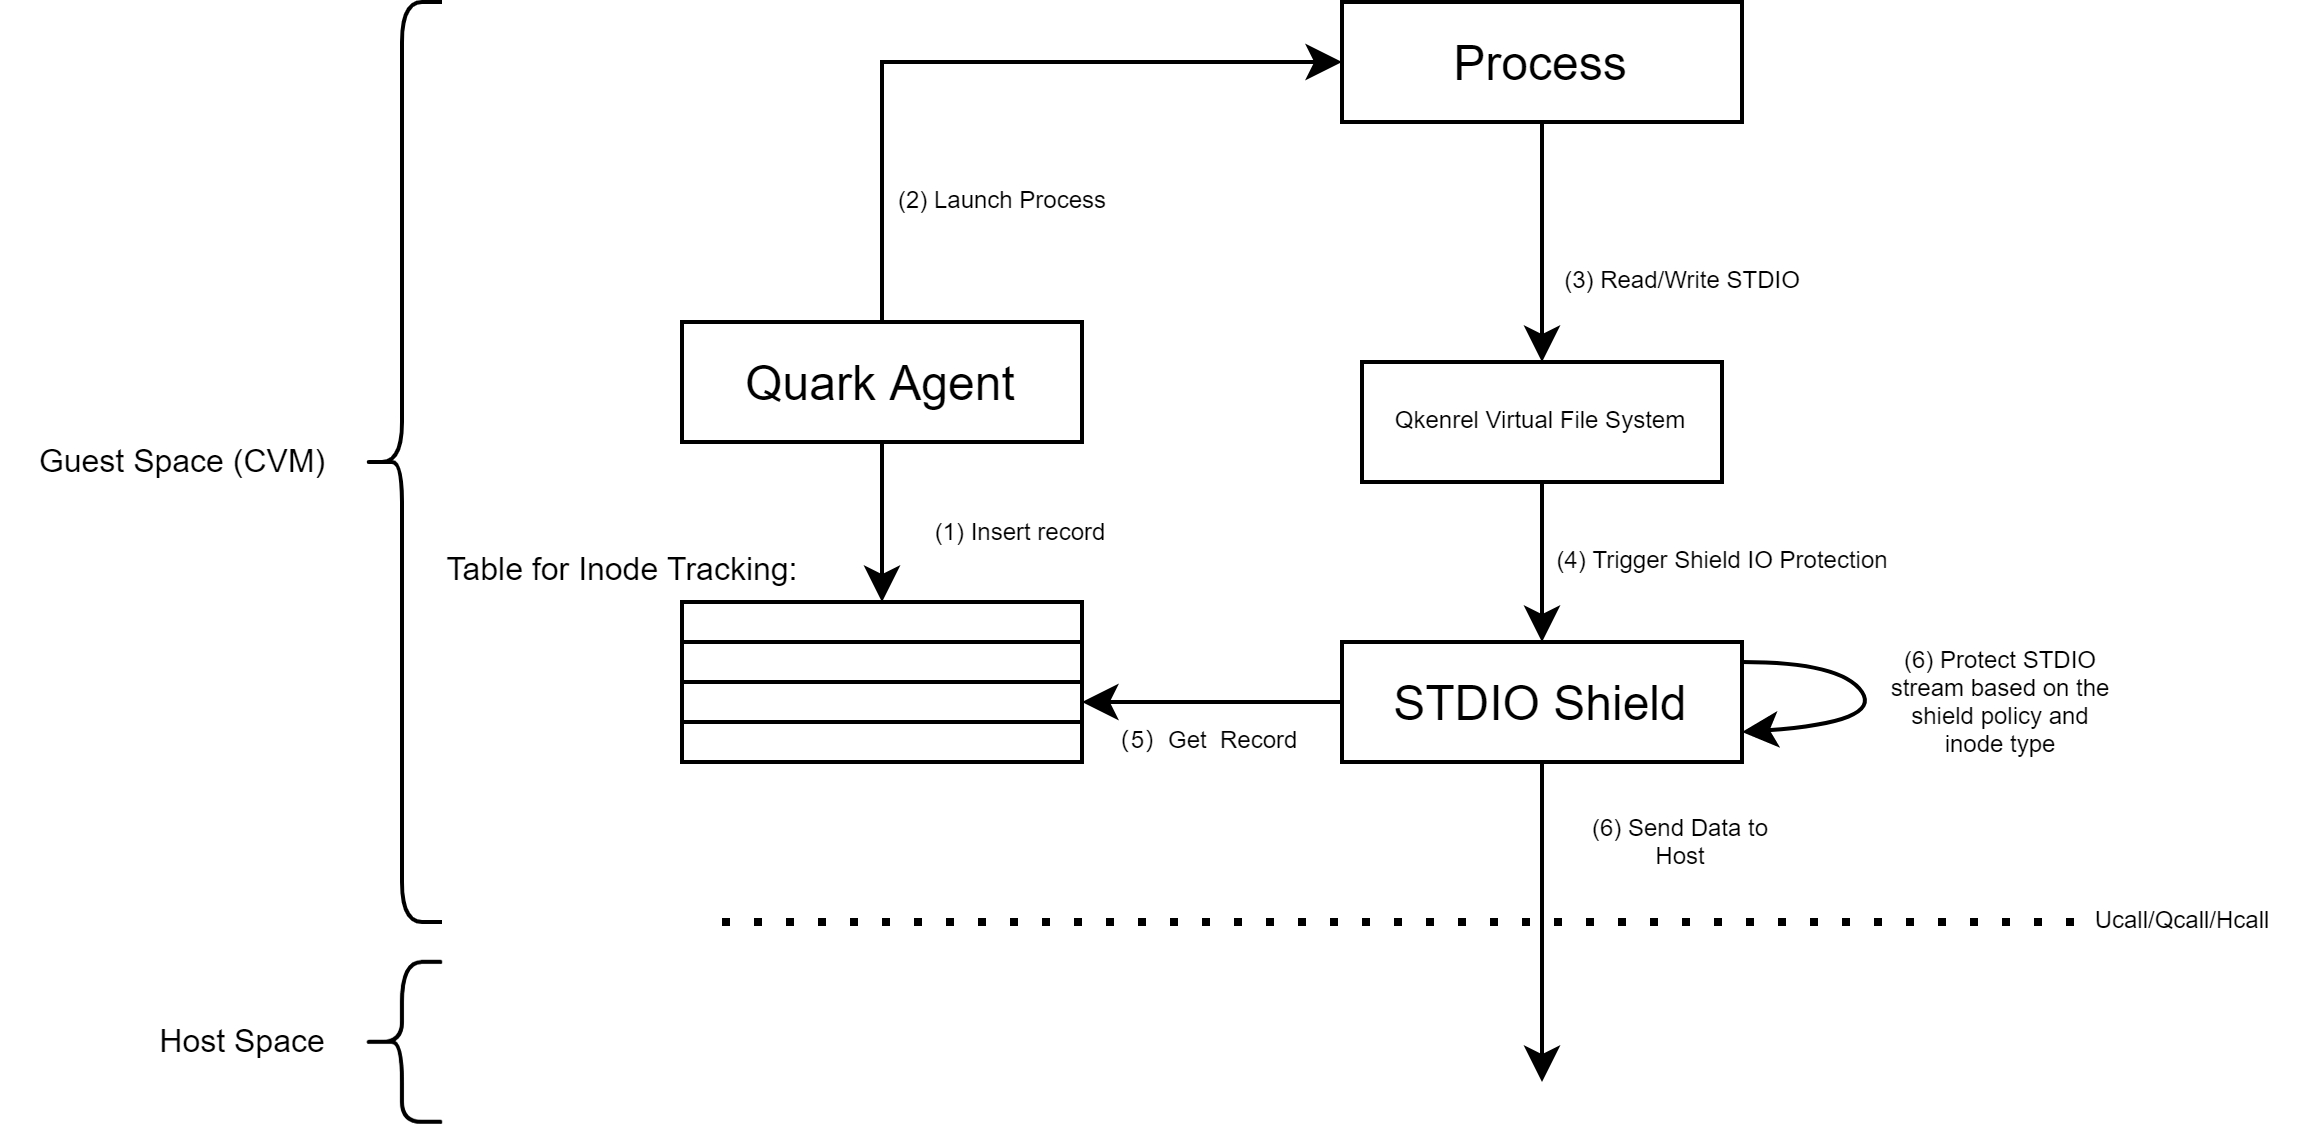
\includegraphics[width=0.8\textwidth]{images/differenciate_fds.png}
    \caption[Inode tracking table workflow]{Inode tracking table workflow}
    \label{fig:differenciate_fds}
\end{figure}
 
The STDIO shield maintains an inode table to track individual processes' STDIN, STDOUT, and STDERR. Each table entry records include the type of STDIO stream, the process's privilege level, the process type, and additional metadata. The available STDIO types consist of STDIN, STDOUT, and STDERR. Process privilege levels are classified as 
privileged or unprivileged. Process types encompass the application, interactive EXEC, non-interactive EXEC, policy update, and session assignment. An entry also includes a session ID and counter if the process type is session assignment. Additionally, for policy update processes, the entry contains a boolean 
value indicating the success of the update. Like session assignment, the STDIO shield informs the user of the policy update result by substituting the data written to the STDOUT of the policy update process.

As shown in Figure~\ref{fig:differenciate_fds}, when the Quark agent creates a process and configures its STDIN, STDOUT, and STDERR file descriptors, corresponding records are created in the inode tracking table. When a process performs read or write operations on its STDIO, the STDIO shield can locate the corresponding inode based on the file descriptor associated 
with the STDIO stream. By utilizing the inode id, the shield can retrieve the relevant record from the inode table and secure the data within the STDIO stream based on the shield policy.

\subsection{Non-interactive process STDIO Protection}

\begin{figure}[!htb]
    \centering
    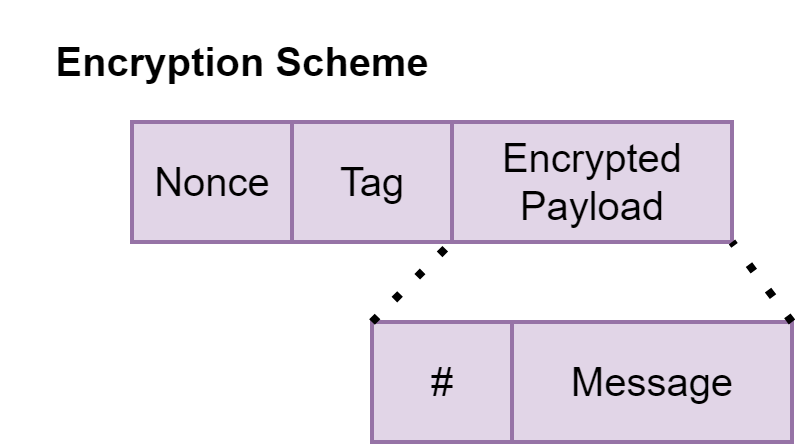
\includegraphics[width=0.3\textwidth]{images/normal_io_shiled_encryption_schema.png}
    \caption[Normal STDIO protection schema]{Normal STDIO protection schema}
    \label{fig:normal_io_shiled}
\end{figure}

Protecting the confidentiality and integrity of the data in the STDERR and STDOUT of privileged-level non-interactive processes is critical. To this end, the Normal STDIO shield utilizes a frame structure in Figure~\ref{fig:normal_io_shiled} to cryptographically protect data written to the STDOUT and STDERR of these processes. The structure consists of an 
encrypted payload, a nonce, and an authentication tag. AES-GCM uses the nonce and the tag for decryption and authentication. The STDIO shield encrypts the payload using the key provided in the enclave policy. Since only the enclave and the enclave owner know the key, an attacker cannot decrypt the encrypted payload. Additionally, the use of AES-GCM ensures the 
confidentiality, integrity, and authenticity of the data. The plaintext payload comprises the data written into STDOUT or STDERR by these processes and a number used to prevent reorder or replay attacks. If a privileged user uses securectl to access an application’s logs, this number is utilized to verify whether the log has been reordered or lost. For privileged-level EXEC processes, this number is the counter’s value 
in the EXEC request. Upon receiving the EXEC result, securectl compares the reference value to the number in the payload to prevent replay attacks.


\subsection{Interactive process STDIO Protection}
\label{subsec:design_terminal}


The goal is to ensure the confidentiality and integrity of the data within the STDIN, STDOUT, and STDERR streams of an interactive process. Achieving this requires end-to-end encryption and decryption of the process's STDIO. Specifically, the data written to STDIN is encrypted by the securectl on its side and decrypted within the enclave. Similarly, 
the STDOUT and STDERR data are encrypted within the enclave and decrypted by the securectl. As discussed in Section~\ref{sec:security_analyse_STDIO}, Quark uses the terminal I/O redirection thread in Quark-shim and the host tty drive to facilitate the STDIO handling. Since the data written by securectl to STDIN is encrypted, the terminal I/O redirection thread cannot filter signals.

For this reason, the terminal I/O redirection thread is merged into the STDIO shield in the enclave. Upon receiving the encrypted data, the STDIO shield reads it from the named pipe representing the process's STDIN, decrypts it, and filters out possible signals. The remaining data is then forwarded to the tty master for further processing. It is important 
to note that the data written to the host tty driver must be encrypted since the enclave does not trust the host. However, this encryption significantly impacts performance and can cause issues with the proper functioning of the tty driver, leading to a malfunctioning terminal.

\begin{figure}[!htb]
    \centering
    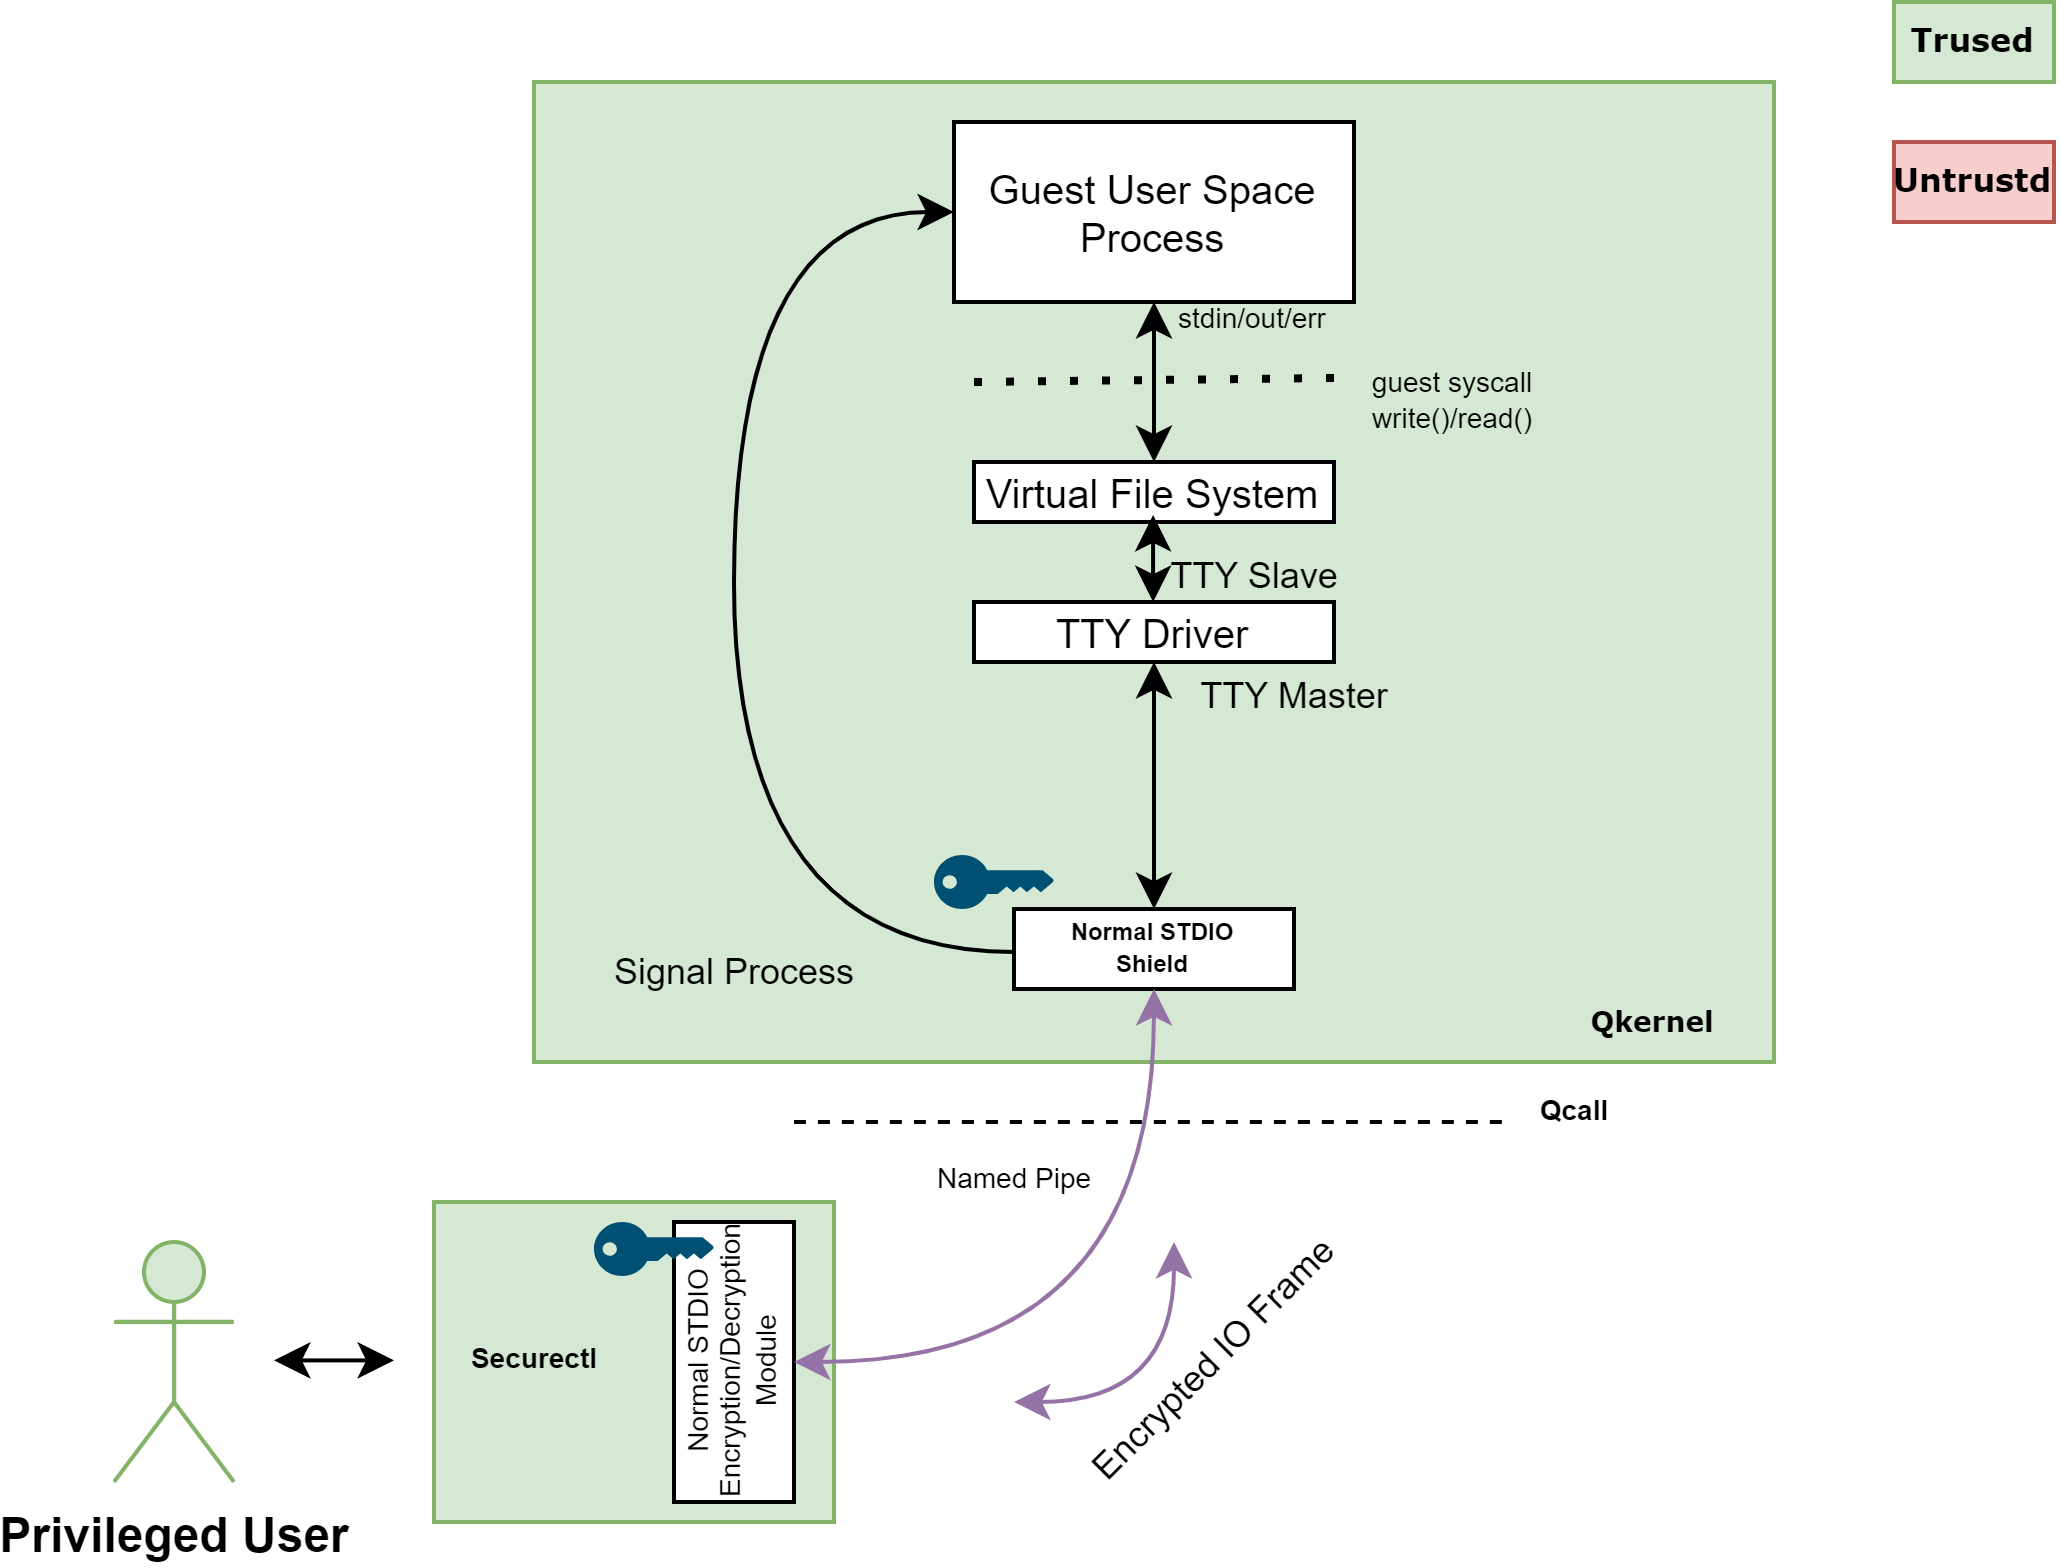
\includegraphics[width=0.6\textwidth]{images/terminal_shiled3.png}
    \caption[Terminal STDIO Protection in case of using Qkernel TTY driver]{Terminal STDIO Protection in case of Qkernel TTY driver}
    \label{fig:terminal_shiled3}
\end{figure}

To address this problem, as depicted in Figure~\ref{fig:terminal_shiled3}, a tty driver must be implemented in the enclave that functions similarly to the host kernel tty driver. This tty driver will handle character echoes, conversion between line feeds and carriage returns, and buffering data written to the tty master. For instance, when a guest userspace 
process writes data to its STDOUT, the write system call handler will redirect the data to the Qkernel tty driver. The tty driver processes the data, transmits it to the tty master, and then alerts the shield to initiate further processing. Following that, the shield encrypts the data extracted from the tty master and transfers it through the Qcall interface to 
securectl.  Securectl then decrypts the data before transmitting it to the user terminal. Upon receiving data from the STDIN-named pipe, the STDIO shield decrypts it and forwards the decrypted data to the TTY driver for further processing. When the user presses '\textbackslash r', the TTY driver transfers its buffered data to the interactive process. It is important to note 
that the STDIO shield applies the same data encryption scheme to both the interactive and non-interactive processes' STDIO.

\subsection{Limitations and Policy for STDIO Shield}
The design of Section~\ref{subsec:design_terminal} has yet to be implemented due to the complexity of the interactive process shield. Consequently, this poses two issues. Firstly, the logs of the interactive application are in plaintext. Secondly, anyone can attach to the interactive application and execute commands. Therefore, as a temporary mitigation, the data written to the STDOUT 
and STDERR of the interactive application process is encrypted using the schema outlined in section 4. This ensures that the interactive application's logs are encrypted. Although an attacker could attach to an interactive application and issue commands, they would not gain any valuable information because the results returned by the application are encrypted.
 
Currently, the STDIO Shield will encrypt the STDIO of userspace processes based on the enclave policy depicted in Figure~\ref{fig:stdio_policy}. If no\_interactive\_process\_stdout\_err\_encryption is true, the STDIO Shield will encrypt the STDOUT and STDERR of all 
non-interactive privilege processes. When interactive\_porcess\_stdout\_err\_encryption is true, the STDIO Shield encrypt STDOUT and STDERR for interactive privilege processes.

\begin{figure}[!htb]
    \centering
    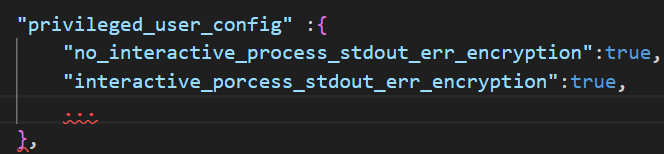
\includegraphics[width=0.6\textwidth]{images/stdio_policy.png}
    \caption[Policy for STDIO shield]{Policy for STDIO shield}
    \label{fig:stdio_policy}
\end{figure}


\section{System Call Interceptor}
\label{sec:design_Interceptor}
\begin{figure}[!htb]
    \centering
    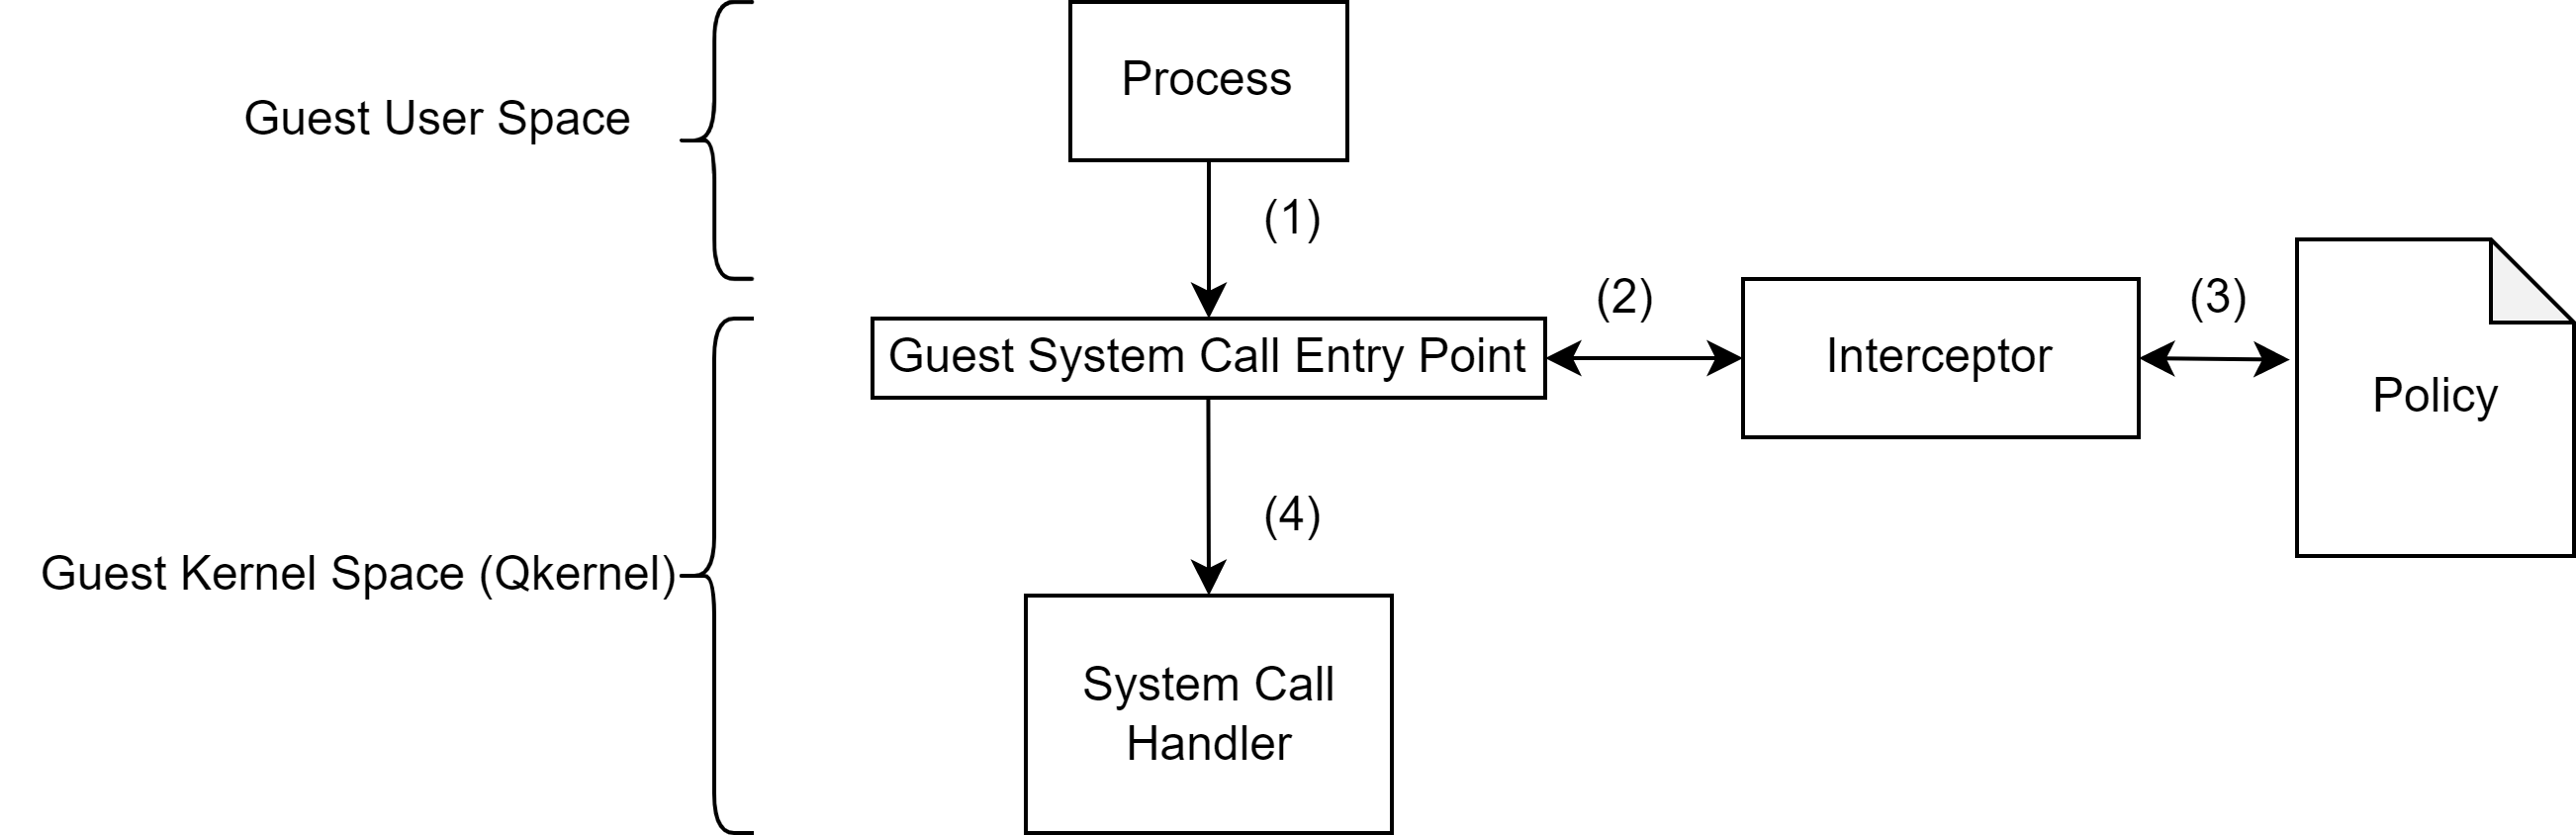
\includegraphics[width=0.8\textwidth]{images/syscall_interceptor.png}
    \caption[System call interceptor workflow]{System call interceptor workflow}
    \label{fig:syscall_interceptor}
\end{figure}
A system call interceptor is implemented in Qkernel, as illustrated in Figure~\ref{fig:syscall_interceptor}. When a guest system call is invoked, the CPU jumps to the guest system call entry point. This entry point is responsible for finding the system call handler in the Qkernel based on the system 
call ID. However, before it does so, it must call the interceptor. The interceptor decides whether the system call is allowed based on the shielding layer's policy. If the system call is not permitted, the guest system call entry point returns EPERM instead of calling the 
system call handler.

\begin{figure}[!htb]
    \centering
    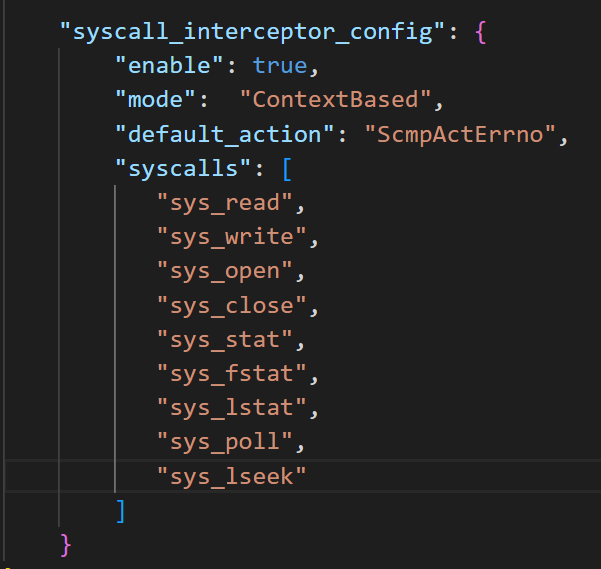
\includegraphics[scale=0.4]{images/policy_system_call.png}
    \caption[System call interceptor's policy]{System call interceptor's policy}
    \label{fig:policy_system_call}
\end{figure}

The interceptor policy is part of the enclave policy and is displayed in Figure~\ref{fig:policy_system_call}. When the keyword "enable" determines whether the interceptor is enabled. The keyword mode specifies the system interceptor's mode: ContextBased or GlobalBased. In GlobalBased mode, the interceptor 
functions across all guest processes, while in ContextBased mode, it operates exclusively for the application process. Considering the potential presence of multiple processes in the guest user space, it is strongly recommended to employ GlobalBased mode. Currently, the system 
interceptor supports only the action, ScmpActErrno, which entails rejecting system calls when their IDs are absent from the allowlist termed "syscalls."





\section{Qkernel Log Manager}
\label{sec:Qkernel_logger}
A Qkernel log manager is implemented to the address issue \ref{vulnerabilities:12}. It can be configured utilizing the enclave policy, exemplified in Figure~\ref{fig:qkernel_Log_config}. The keyword enabled determines whether the manager is enabled. When set to false, the Qkernel log system employs the logging level specified in 
the Qkernel configuration file. Furthermore, the keyword "allowed\_max\_log\_level" designates the maximum log level Qkernel can print. As discussed in Section~\ref{sec:Qkernel_Log_Misconfiguration}, Qkernel supports five log levels. For instance, when "allowed\_max\_log\_level" is set to INFO, Qkernel is exclusively restricted to printing 
logs at the INFO and ERROR levels. Additionally, the enclave policy is passed to the enclave during application deployment. Until the enclave obtains the policy, the Qkernel log manager is enabled and employs the log level OFF.
\begin{figure}[!htb]
    \centering
    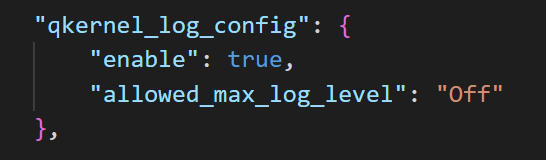
\includegraphics[width=0.4\textwidth]{images/qkernel_Log_config.png}
    \caption[Qkernel log manager's policy]{Qkernel log manager's policy}
    \label{fig:qkernel_Log_config}
\end{figure}

\section{Modification to OCI}
\label{sec:Modification_OCI}

\subsection{Extending the container lifecycle to support confidential computing}
The container lifecycle definition in the OCI RUNTIME specification~\cite*{oci-runtime-spec} lacks support for remote attestation and protection for the application’s STDIO. In this section, we first define container runtime and enclave in the context of confidential computing. Then we will propose modifications to the container 
lifecycle.


\subsubsection{Definition of Runtime and Enclave in Confidential Computing}

Currently, the container runtime in the OCI runtime specification~\cite*{oci-runtime-spec} refers to the runtime environment used to create containers. A VM-based container runtime includes the shim process, the hypervisor, and the agents inside the guest used to create and manage containers. 
For example, in the kata container, these three components correspond to kata-shim, qemu, and kata-agent, respectively. However, in confidential computing, the runtime is divided into two parts: the trusted agent, the untrusted shim process, and the hypervisor. Therefore, we redefine 
the runtime as untrusted runtime components, including the shim and hypervisor. In addition, we refer to the guest as an enclave containing the agent, guest kernel, etc.

\subsubsection{Modification to Container Lifecycle}
We make the following changes to the container lifecycle. Note that the bold text in the list is the part we modified, the rest is copied from OCI RUNTIME SPECIFICATION~\cite*{oci-runtime-spec}.

\begin{enumerate}
    \item OCI compliant runtime's create command is invoked with a reference to the location of the bundle and a unique identifier.
    \item The container's runtime environment and enclave MUST be created according to the configuration in config.json. If the runtime is unable to create the environment specified in the config.json, it MUST generate an error. While the resources requested in the config.json MUST be created, the user-specified program (from process) MUST NOT be run at this time. Any updates to config.json after this step MUST NOT affect the container
    \item The prestart hooks MUST be invoked by the runtime. If any prestart hook fails, the runtime MUST generate an error, stop the container, and continue the lifecycle at step 16
    \item The createRuntime hooks MUST be invoked by the runtime. If any createRuntime hook fails, the runtime MUST generate an error, stop the container, and continue the lifecycle at step 16.
    \item The createContainer hooks MUST be invoked by the runtime. If any createContainer hook fails, the runtime MUST generate an error, stop the container, and continue the lifecycle at step 14.
    \item Runtime's start command is invoked with the unique identifier of the container.
    \item The startContainer hooks MUST be invoked by the runtime. If any startContainer hook fails, the runtime MUST generate an error, stop the container, and continue the lifecycle at step 14.
    \item \textbf{The Enclave receives the runtime’s start request and constructs a process for the user-specified program, as specified by process. If this hook fails, the enclave MUST generate an error, stop the container, and continue the lifecycle at step 16}
    \item \textbf{The enclave Must invoke the application launch measurement hook if the user-specified program’s binary is loaded from the host. If this hook fails, the enclave MUST generate an error, stop the container, and continue the lifecycle at step 16.}
    \item \textbf{The attestation and provisioning hook MUST be invoked within the enclave when the enclave finish loading the program’s binary. If this hook fails, the enclave MUST generate an error, stop the container, and continue the lifecycle at step 16.}
    \item \textbf{The application rocess enters user space and starts to run.}
    \item \textbf{The enclave MUST invoke the runtime measurement hook when the program process loads binary or shared library from the host. If this hook fails, the enclave MUST generate an error, stop the container, and continue the lifecycle at step 16}
    \item \textbf{The enclave MUST invoke the STDIO protection hook when the program/exec process reads or writes data from its standard IO. If this hook fails, the enclave MUST generate an error, stop the container, and continue the lifecycle at step 16}
    \item The poststart hooks MUST be invoked by the runtime. If any poststart hook fails, the runtime MUST log a warning, but the remaining hooks and lifecycle continue as if the hook had succeeded.
    \item The container process exits. This MAY happen due to erroring out, exiting, crashing or the runtime's kill operation being invoked.
    \item Runtime's delete command is invoked with the unique identifier of the container.
    \item The container MUST be destroyed by undoing the steps performed during create phase (step 2).
    \item The poststop hooks MUST be invoked by the runtime. If any poststop hook fails, the runtime MUST log a warning, but the remaining hooks and lifecycle continue as if the hook had succeeded.    
  \end{enumerate}

  The application launch measurement hook should be called when the enclave loads the application binary from the host. This hook must be executed in the enclave namespace. It measures the binaries loaded from the host before the application process starts. The attestation and provisioning hook will add the measurement result to attestation evidence and then 
  forward it to the relying party for integrity check. Note that the TEE hardware must measure this hook as part of the enclave container runtime component.
 
  The attestation and provisioning hook must be invoked after the enclave loads the application binary but before the application process stack is set. The enclave uses this hook to authenticate itself to the relying party and retrieve the secrets. A reference design can be found in Section~\ref{sec:secure_application_deployment}. Note that this hook must be executed in the enclave 
  namespace. After the attestation and provisioning hook retrieves the secrets, the environment variable and application parameter type secrets should be pushed into the application process's stack. The enclave should store the file type secret in a trusted environment, such as enclave memory. 
   
   
  The enclave should call the runtime measurement hook when the application loads a shared library or binary file from the host at runtime. This hook must be executed in the enclave namespace. It forces the integrity check on the loaded shared library or binary against a reference value obtained from relying party.    
   
   
  The STDIO protection hook should be invoked when an application or a privileged exec process reads or writes its STDIO. It encrypts the privileged process's STDIN, STDOUT, and STDERR based on policy obtained from relying party. A reference design can be found in Section~\ref{sec:design_STDIO_PROTECTION}.
   
  The attestation and provisioning hook, runtime measurement hook, and STDIO Protection hooks may be included as part of the enclave's operating system or loaded from the host after the enclave starts. In the former case, these hooks will be measured by the TEE hardware or bootloader. In the latter case, The application launch measurement hook should measure 
  these hooks. 
\subsection{EXEC Operating Guidelines}

The OCI runtime specification intentionally refrains from standardizing the EXEC operation to provide developers with flexibility~\cite*{exec_semantics}. However, in confidential computing scenarios, the EXEC operation allows attackers to acquire application secrets, thereby compromising confidentiality. As a result, we advocate for the standardization of the 
EXEC operation in confidential computing scenarios.
 
We utilize the proposal depicted in Figure~\ref{fig:exec_propose} as a foundation for standardization. This proposal was initially submitted to the OCI Runtime spec forum, although it was ultimately not accepted due to the previously outlined reason.
 
\begin{figure}[!htb]
    \centering
    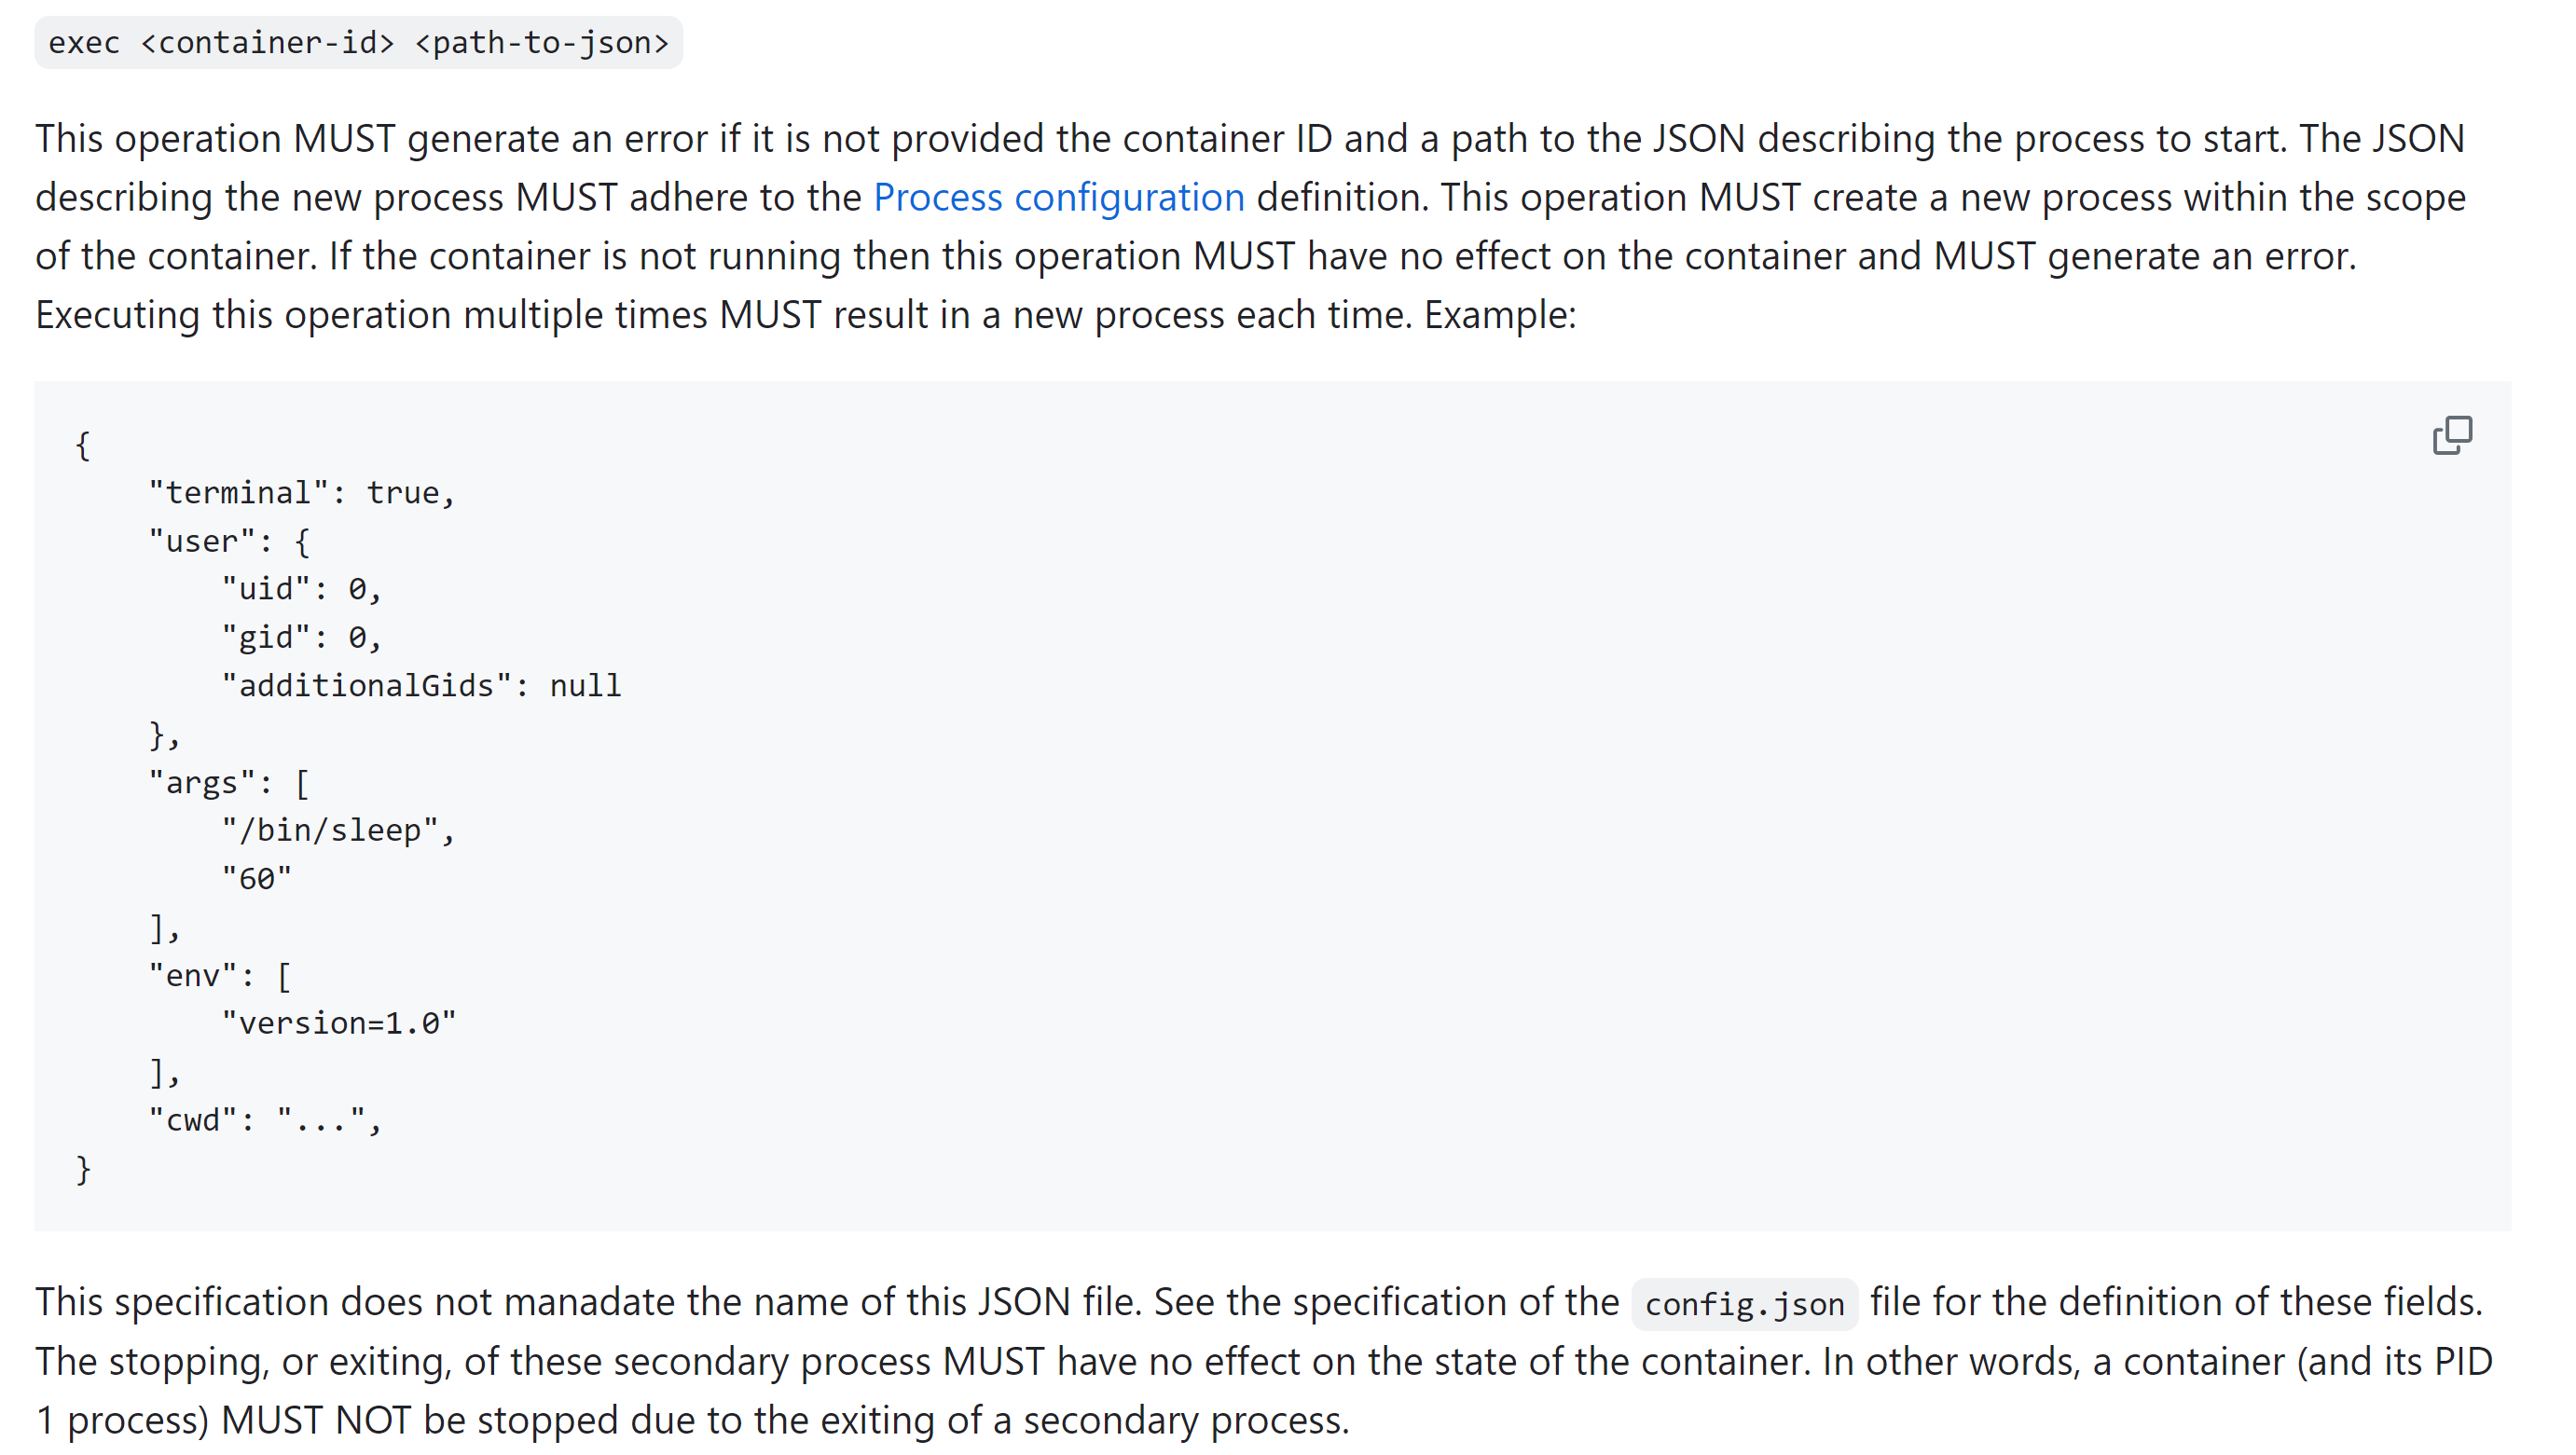
\includegraphics[width=0.8\textwidth]{images/exec_propose.png}
    \caption[Proposal for standardizing EXEC operation]{Proposal for standardizing EXEC Operation from~\cite*{exec_proposal} }
    \label{fig:exec_propose}
\end{figure}
 
In the confidential computing scenario, EXEC requests should be categorized into privileged requests issued by the application owner and unprivileged requests issued by others. The method discussed in Section~\ref{sec:design_prptect_privileged_request} is employed to protect the args array in the EXEC specification (Figure~\ref{fig:exec_propose}). This way, 
we can differentiate between privileged and non-privileged requests and ensure the confidentiality and integrity of privileged commands. This method necessitates sharing a symmetric key between the privileged user and the enclave. The enclave can obtain this key through the remote attestation and provisioning hook. Prior to creating an EXEC process,
the enclave must authenticate and control access to the request based on the policy shown in Figure~\ref{fig:exec_policy}. The authentication and access control workflow can be found in section~\ref{sec:impl_exec}. Additionally, to safeguard the results of privileged EXEC requests, the enclave must encrypt the data written to the STDOUT and STDERR of a 
privileged process. The encryption mechanism is explained in Section~\ref{sec:design_STDIO_PROTECTION}.


  

\section{Summary}
In this chapter, we present mechanisms for protecting the integrity and confidentiality of a secure application's secrets when it is orchestrated by untrusted k8s. We demonstrate a secure approach to deploying applications, and how to protect 
the confidentiality and integrity of the application's standard flows, restrict the commands users can issue to the application, and propose modifications to the OCI interface. With these approach, applications can be orchestrated in a secure 
manner by untrusted entities. In next chapter, we describe how we implemented this mechanisms .
\cleardoublepage

%%% Local Variables:
%%% TeX-master: "diplom"
%%% End:

\chapter{Implementation}
\label{sec:implementation}

% Hier greift man einige wenige, interessante Gesichtspunkte der
% Implementierung heraus. Das Kapitel darf nicht mit Dokumentation oder
% gar Programmkommentaren verwechselt werden. Es kann vorkommen, daß
% sehr viele Gesichtspunkte aufgegriffen werden müssen, ist aber nicht
% sehr häufig. Zweck dieses Kapitels ist einerseits, glaubhaft zu
% machen, daß man es bei der Arbeit nicht mit einem "Papiertiger"
% sondern einem real existierenden System zu tun hat. Es ist sicherlich
% auch ein sehr wichtiger Text für jemanden, der die Arbeit später
% fortsetzt. Der dritte Gesichtspunkt dabei ist, einem Leser einen etwas
% tieferen Einblick in die Technik zu geben, mit der man sich hier
% beschäftigt. Schöne Bespiele sind "War Stories", also Dinge mit denen
% man besonders zu kämpfen hatte, oder eine konkrete, beispielhafte
% Verfeinerung einer der in Kapitel 3 vorgestellten Ideen. Auch hier
% gilt, mehr als 20 Seiten liest keiner, aber das ist hierbei nicht so
% schlimm, weil man die Lektüre ja einfach abbrechen kann, ohne den
% Faden zu verlieren. Vollständige Quellprogramme haben in einer Arbeit
% nichts zu suchen, auch nicht im Anhang, sondern gehören auf Rechner,
% auf denen man sie sich ansehen kann.

%\ldots implementation \ldots

The chapter outlines the implementation of the shielding layer. Firstly, it illustrates the implementation of the quark attestation and provisioning infrastructure (Section~\ref{sec:impl_attestation_infr}). This includes the communication establishment between the attestation and provisioning agent 
with the secret manager, the way the secret injector deploys secrets, the runtime attestation service's implementation, and how the attestation driver acquires attestation reports from \acrshort{TEE}. Secondly, it details the implementation of the software measurement manager (~\ref{sec:impl_measurement}). 
Section~\ref{sec:impl_exec} presents the EXEC checker's steps for checking an exec request. Finally, sections~\ref{sec:impl_STDIO},~\ref{sec:impl_interceptor}, and~\ref{sec:iml_qlog} explain the implementation of the process's STDIO protection, system call 
interceptor, and the Qkernel log manager, respectively. The source code is accessible on GitHub~\cite*{theis_source_code}.

\section{Quark Attestation and Provisioning Infrastructure}
\label{sec:impl_attestation_infr}

\subsection{Secret Uploading}
The secret manager must operate within the application owner's local environment. It implements a local file system backend. The application owner can deploy secrets to a path the secret manager can find using a script~\cite*{secret_uploading_script}. The functionality to create a secure channel 
based on TLS~\cite*{tls_record_size} and attestation and then upload secrets still needs to be implemented.

\subsection{Attestation and Provisioning Agent}
The attestation and provisioning agent is an HTTPS client designed to provide the enclave with the following interface to prove its identity to the secret manager and fetch secrets.

\begin{lstlisting}[language=rust, caption= API of the atestation and provisioning agent]
    pub fn provisioning_http_client(task: &Task, software_maasurement: &str, sm_cert: Vec<u8>) -> Result<(KbsPolicy, KbsSecrets)>
\end{lstlisting}

The function takes the enclave startup hash and the secret manager’s public key as arguments and returns the enclave policy and application’s secrets if attestation succeeds. Note that this function is called only after loading the application binary because the enclave startup hash is 
generated afterward. This function solves the following three problems:

\begin{enumerate}
    \item How the agent establishes a TCP connection to the secret manager
    \item How the agent establishes a TLS channel on top of the TCP connection to the secret manager
    \item How the agent constructs HTTP requests according to the KBS attestation protocol, proves its identity to the secret manager, and retrieves secrets.
\end{enumerate}

\subsubsection{TCP connection establishment}

Listing~\ref{lst:api_for_tcp_connection} shows the API for establishing the TCP connection. To make the Qkernel socket object available to the shield layer, we implement the Provider interface define in the Qkernel network stack for the ShieldSocketProvider. Since each socket implements trait SockOperations, the shielding layer can 
first use ShieldSocketProvider to obtain a socket object and then use Connect() method to connect the socket to the secret manager.

\begin{lstlisting}[language=rust, caption= API for establishing the TCP connection, label={lst:api_for_tcp_connection}]
pub struct ShieldSocketProvider {
    pub family: i32,
}

impl Provider for ShieldSocketProvider {
    fn Socket(...) -> Result<Option<Arc<File>>>;
}

pub trait SockOperations: Sync + Send {
    fn Connect(...) -> Result<i64> {}
…
}    
\end{lstlisting}

\subsubsection{TLS channel establishment}
Listing~\ref{lst:api_for_tls_connection} shows the functions for creating a TLS channel. We use no-std compatible crate embedded-tls~\cite*{embede_tls}  to establish a TLS channel between the secret manager and the enclave, as Qkerenl runs in a no-std environment. The socket connected to the secret manager is stored in 
ShieldProvisioningHttpSClient. Therefore, we implement embedded\_io::blocking::Read and embedded\_io::blocking::Write for ShieldProvisioningHttpSClient. The embedded-tls library can then use the functions in these two traits to read and write 
the socket stored in ShieldProvisioningHttpSClient.

\begin{lstlisting}[language=rust, caption= API for establishing the TLS channel, label={lst:api_for_tls_connection}]
pub struct ShieldProvisioningHttpSClient {
    pub socket_file: Arc<File>,
    ...
}

impl embedded_io::blocking::Read for ShieldProvisioningHttpSClient {
    fn read<'m>(&'m mut self, read_to: &'m mut [u8]) -> Result<usize>;
}

impl embedded_io::blocking::Write for ShieldProvisioningHttpSClient {
    fn write<'m>(&'m mut self, write_from: &'m [u8]) -> Result<usize>;
}
\end{lstlisting}
\subsubsection{Building HTTP requests according to the KBS attestation protocol}
Listing~\ref{lst:http_connection} shows the functions for constructing the HTTP requests defined in the KBS attestation protocol~\cite*{kbs_Attestation_protocol}. ShieldProvisioningHttpSClient holds the metadata used in the protocol. The explanation of those data can be found in section~\ref{sec:kbs};


The functions prepair\_post\_auth\_http\_req, prepair\_post\_attest\_http\_req, and prepair\_get\_resource\_http\_req are employed to construct the HTTP request string defined in the KBS attestation protocol, i.e., "Post /kbs/v0/auth", "Post /kbs/v0/attest", and "GET /kbs/v0/<resource\_id>". 
The generated string is submitted to the embedded-tls library~\cite*{embede_tls} by the function send\_http\_request\_to\_sm. The embedded-tls library wraps the string into a TLS record and writes it to the socket stored in ShieldProvisioningHttpSClient via the embedded\_io::blocking::Write 
function. When the secret manager receives the request, it processes the request accordingly and returns the response, which is encapsulated in a TLS record. The embedded-tls library reads the record through the embedded\_io::blocking::Read function, then decrypts it.

The decrypted string is parsed by parse\_auth\_http\_resp , parse\_attest\_http\_resp, or parse\_http\_get\_resource\_resp. These functions first interpret the string according to the HTTP specification. They will then process the HTTP 
response according to the semantics of the KBS attestation protocol~\cite*{kbs_Attestation_protocol}. Specifically, for an HTTP response to Post /kbs/v0/auth, function parse\_auth\_http\_resp will save the cookie and nonce to ShieldProvisioningHttpSClient. For Post /kbs/v0/attest's response, the parse\_attest\_http\_resp function will 
check HTTP response status codes to determine if the attestation is successful. When a GET /kbs/v0/ response is received, the parse\_http\_get\_resource\_resp function is called. It decrypts the payload using the private part of tee\_key, and returns the secret.

Furthermore, the generate\_evidenc function is invoked by the prepair\_post\_attest\_http\_req when generating the Post /kbs/v0/attest request string. It prompts the attestation driver to produce an attestation report. The custom field of the report includes the hash of the nonce, 
the public part of the tee\_key, and the enclave's startup hash.                                                                                                                                                                                                                                                                                                


\begin{lstlisting}[language=rust, caption= Functions for building the HTTP requests defined in the KBS attestation protocol, label={lst:http_connection}]
fn send_http_request_to_sm (...)->  core::result::Result<… >;

pub struct ShieldProvisioningHttpSClient {
    pub socket_file: Arc<File>,
    cookie: String,
    nonce: String,
    tee_key: Option<TeeKey>,
    pub tee_type: Tee,
}

impl ShieldProvisioningHttpSClient {
    fn prepair_post_auth_http_req(&self) -> String;
    fn parse_auth_http_resp(&mut self, resp_buf: &[u8]) -> Result<()>;
    fn prepair_post_attest_http_req(&self, software_maasurement: &str) -> Result<String>;
    fn parse_attest_http_resp(&mut self, resp_buf: &[u8]) -> Result<()>;
    fn prepair_get_resource_http_req(&self, resource_url: String) -> String;
    fn parse_http_get_resource_resp(&mut self, resp_buf: &[u8]) -> Result<Vec<u8>>;
    fn generate_evidence(&self, software_maasurement: &str) -> Result<Attestation>;
}
    
\end{lstlisting}

It is important to note that HTTP requests and responses alike are bound within a strict 16 KB limit, as the maximum TLS record size is 16 KB~\cite*{tls_record_size}. Inevitably, the secret size is also subject to the 16 KB limit. Since file type secrets can be huge, the 
enclave must execute a single HTTP GET request for each file. Generally speaking, the application owner may inject an enclave policy, a file containing environment variables and command line arguments of the application, and n file type secrets into the enclave. 
In this case, the enclave needs to execute n+2 HTTP get requests.

\subsubsection{Limitations}
\label{subsec:Limitations}

The attestation report is fake because the enclave cannot operate within a \acrshort{TEE}. Upon receipt of a POST /kbs/v0/attest request, the secret manager will omit to verify the report signatures and \acrshort{TEE} hardware's measurements for the VM startup. This means the secret manager will not validate the report's 
genuineness and the integrity of the Qkernel binary. Furthermore, the secret manager cannot identify an enclave by examing the enclave id in the host data fields of the report since there is no efficient way to pass the enclave ID to the Qvisor before starting the enclave. As a result, the secret 
manager only validates the custom field in the report, which includes the hash of the nonce, the public part of the tee\_key, and the enclave's startup hash. This ensures that the enclave startup hash is consistent with the reference hash provided by the application owner. Identifying the enclave 
identity, checking the report's signature, and verifying the \acrshort{TEE}'s measurement are left for later implementation.


\subsection{Secret Injector}
The secret injector keeps application secrets and deploys file-type secrets. It has the following API. 
\begin{lstlisting}[language=rust, caption= API for Secret Injector, label={lst:Secret_injector}]
pub struct SecretKeeper {
    pub secrets_mount_info: FileSystemMount,
    pub file_secrets:  BTreeMap<String, Vec<u8>>,  // key: file name, value: secret
    pub arg_env_based_secrets: Option<EnvCmdBasedSecrets>,
}

impl SecretKeeper {
    pub fn set_secrets_mount_info (&mut self, info: FileSystemMount) -> Result<()>
    pub fn bookkeep_secrets (&mut self, secrets: KbsSecrets) -> Result<()>
    pub fn inject_file_based_secret_to_secret_file_system (&self, task: &Task) -> Result<()>
}   
\end{lstlisting}

Function set\_secrets\_mount\_info records information about the application's file system, which can be used to create a sub-filesystem for the file type secrets. As discussed in Section~\ref{sec:design_Quark_Attestation_and_Provisioning_Infrastructure}, the file system is mounted under directory 
/secret. Mounting the file system is facilitated by the function inject\_file\_based\_secret\_to\_secret\_file\_system, which calls the function MountSubmounts in Qkernel. The function bookkeep\_secrets stores the application's secrets in the SecretKeeper. Additionally, since the command-line and environment variable type secrets are pushed onto the application's 
stack,  SecretKeeper does not implement any function to deploy these types of secrets.

\subsubsection{Secret Sub-filesystem}
Listing~\ref{lst:sub_filesystem} presents the API for creating the filesystem for file type secrets. SecretFileSystem implements the  Qkernel's filesystem interface, which can be called by the mountSubmounts() to mount the file secrets to this sub-filesystem.  During this process, 
the Mount function creates an inode for each file type secret stored in SecretKeeper and saves it in a BTreeMap called contents. The BTreeMap is used to initialize the Qkernel object Dir, which represents the directory object in Qkernel. Dir is then used to initialize the inode 
representing the sub-filesystem, i.e., NewSecretInode. Later, MountSubmounts will add this inode to the mounts fields in the structure MountNsInternal, which stands for the application process mount namespace.

\begin{lstlisting}[language=rust, caption= API for secret file system, label={lst:sub_filesystem}]
pub struct SecretFileSystem {}
impl Filesystem for SecretFileSystem {
    fn Mount(&mut self, task: &Task, device: &str, flags: &MountSourceFlags, data: &str) -> Result<Inode> {
            ...
    }
}

pub struct MountNsInternal {
    pub mounts: QMutex<BTreeMap<u64, Arc<QMutex<Mount>>>>,
    ...
}
      
\end{lstlisting}

The Dir and the NewSecretInode object implement the Qkernel InodeOperation trait, as depicted in Listing~\ref{lst:accessing_file}. The function Lookup in the trait helps the Qkernel find the inode corresponding to the secret when the application reads a file under directory /secret. The secret inode also adopts the InodeOperation trait, 
in which GetFile() will return a file object. This file object implements the FileOperations trait. The Qkernel can utilize the ReadAt function in this trait to read the file secret stored in SecretKeeper. Moreover, the file does not implement WriteAt, as the secret sub-filesystem is read-only.

\begin{lstlisting}[language=rust, caption= Interface for accessing the file type secrets, label={lst:accessing_file}]

pub trait InodeOperations: Sync + Send {
    fn Lookup(&self, task: &Task, dir: &Inode, name: &str) -> Result<Dirent>;
    fn GetFile(&self, task: &Task, dir: &Inode, dirent: &Dirent, flags: FileFlags) -> Result<File>;
    ...
}

pub trait FileOperations: Sync + Send + Waitable + SockOperations + SpliceOperations {
    fn WriteAt(&self, task: &Task, f: &File, srcs: &[IoVec],offset: i64,_blocking: bool) -> Result<i64>;
    fn ReadAt(&self,task: &Task,f: &File, dsts: &mut [IoVec],offset: i64, _blocking: bool,) -> Result<i64>;
    ...
}
    
      
\end{lstlisting}

\subsection{Attestation Driver}
\label{subsec:impl_Attestation_driver}
The attestation driver facilitates communication with the AMD SNP to acquire attestation reports. While Qkernel currently does not support running on \acrshort{TEE}, we aim to implement the driver based on the SNP  guest messages protocol~\cite*{snp_firmware} in a simulation environment. Once Qkernel supports 
AMD SNP, the driver can operate directly with the SNP firmware. 


Guest and AMD firmware are communicating following SNP guest messages protocol. During initialization, AMD firmware adds a secret page to the guest's private memory. This page contains four keys, namely, VMPCK0-3~\cite*{snp_firmware}, which the guest and the AMD firmware share. Using the VMPCK encryption,  the guest 
can initiate an SNP guest request with an encrypted payload and relay the request to the SNP through the hypervisor. Subsequently, the SNP decrypts the request with the proper VMPCK and completes the request. These requests include generating a key, creating an attestation report, etc. The key and 
report are encrypted by VMPCK and returned to the guest via the SNP response. The guest can decrypt the response to get the corresponding data.

\begin{figure}[htp]
    \centering
    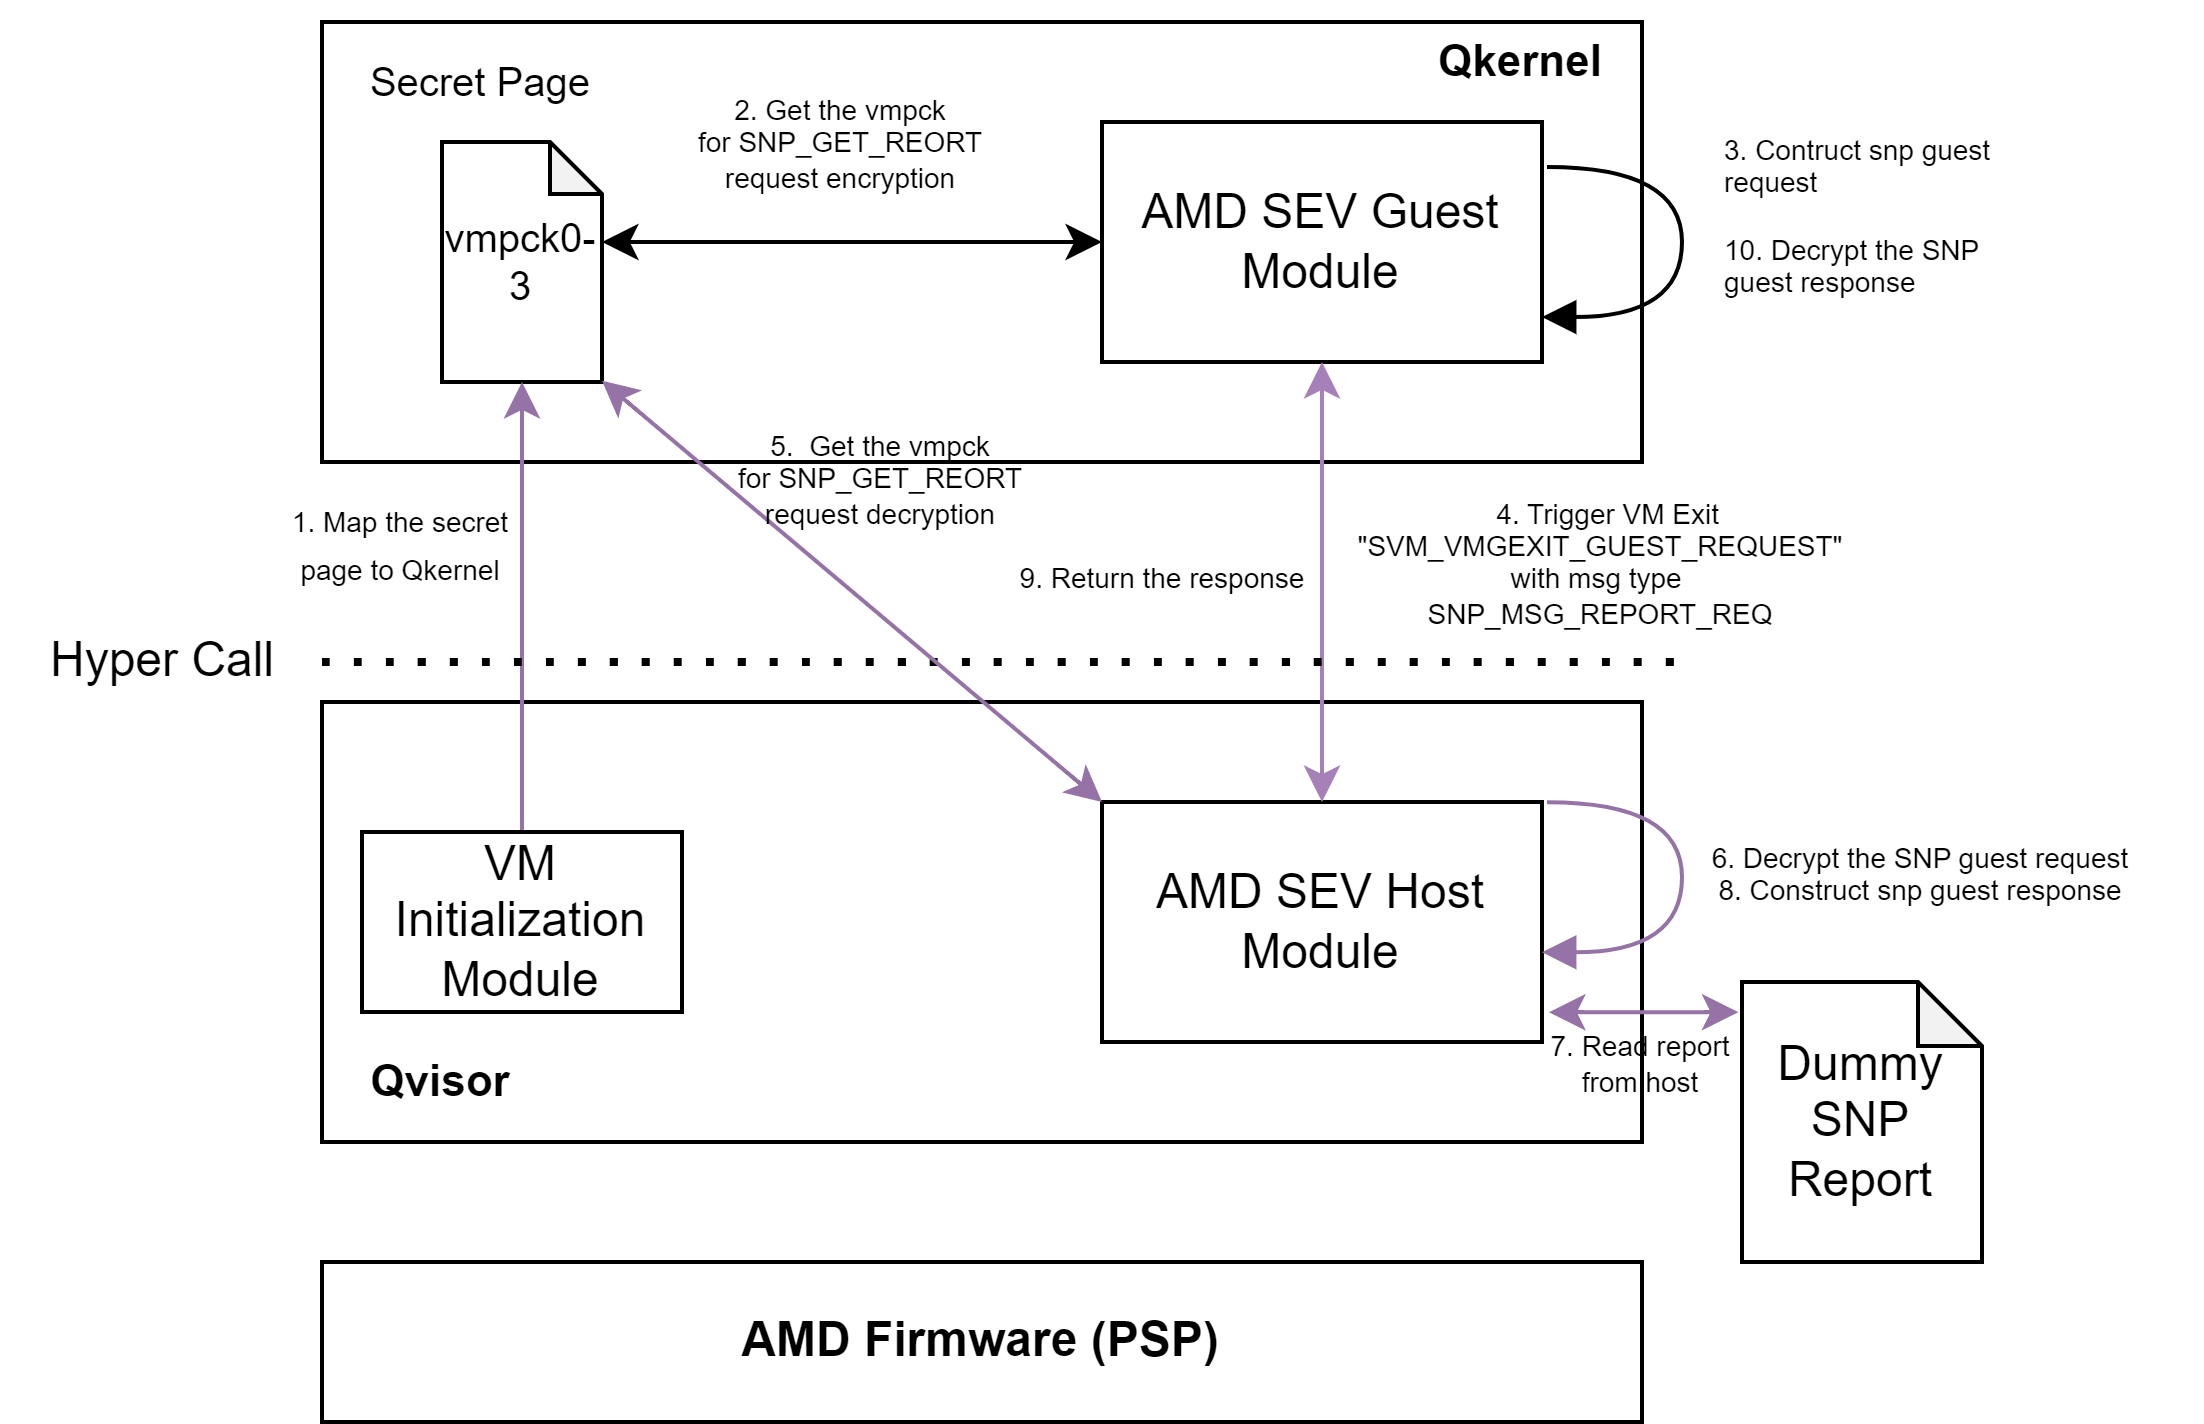
\includegraphics[width=0.8\textwidth]{images/amd_snp_driver.png}
    \caption[Attestation Driver Workflow]{Attestation Driver Workflow}
    \label{fig:amd_snp_driver}
\end{figure}

To simulate the process above, as shown in Figure~\ref{fig:amd_snp_driver}, Qvisor's VM initialization module initializes a secret page during the virtual machine's creation process. This page is mapped to shared memory between Qvisor and Qkernel. When the enclave requests an attestation 
report, the attestation driver creates an  SNP request using a VMPCK on the secret page. This request is relayed to the AMD SEV SNP firmware emulation module in Qvisor via the hypercall SVM\_VMGEXIT\_GUEST\_REQUEST. This module emulates SNP firmware. It will decrypt the request 
using the VMPCK on the page. A dummy report is then retrieved from the disk and tweaked according to the attestation driver's requirements for the user-defined field. Subsequently, the SNP module encrypts the altered report with VMPCK and returns it to the attestation driver as the SNP response payload. The attestation driver can 
decrypt the response and retrieve the report using VMPCK.

This driver provides the API in Listing~\ref{lst:Attestation_driver} . It takes user-defined data and returns a report serialized as a JSON string. The user-defined data is added to the custom field of the report. Returning a string instead of a specific report allows extending this driver to support multiple \acrshort{TEE}s. Specifically,  
when it receives a request to generate a report, it will generate a report in different formats depending on the type of \acrshort{TEE}. Then, it will serialize this report into a string and return it to the requestor. The requestor can deserialize this string to get the specific report according to the \acrshort{TEE} type
\begin{lstlisting}[language=rust, caption= API of attestation driver, label={lst:Attestation_driver}]
pub fn get_report(&mut self, report_data: String) -> Result<String>   
\end{lstlisting}

\subsection{Runtime Attestation Service}
The API of the runtime attestation service is shown in the Listing~\ref{lst:runtime_attestation}. We have added a new system call with id 451 to the Qkernel. The SysAttestationReport function is the handler for this system call. It accepts parameters, user-defined data, data length, and Request structure and returns a report to 
the application. Here, the Request allows the application to specify the desired report type.

\begin{lstlisting}[language=rust, caption= Interface for accessing the file type secrets, label={lst:runtime_attestation}]

pub struct Requst {
    pub software_based_report_requered: bool,
    pub use_user_provided_signing_key: bool,
    pub signing_key_length: usize, 
    pub signing_Key: [u8; 4096],  
}

pub struct Report {
    //  AMD SNP: 2, TDX: 3, Software based: 4
    pub tee_type: u64,
    pub report_length: u64,
    //  AMD SNP REPORT has 1183 bytes, INTEL TDX report has 1024 bytes
    pub report: [u8; 4096],  
}

pub fn SysAttestationReport(task: &mut Task, args: &SyscallArguments) -> Result<i64>      
\end{lstlisting}

SysAttestationReport can generate software or hardware reports. In order to return a report of any type, the function serializes a report as a JSON string. It then converts the string into a byte array and embeds the array in the report field of the Report structure. After that, SysAttestationReport copies 
the Report structure to the address specified by the application. The application can get the length of the report character array from the report\_length in the Report structure. After converting the report character array to a string, the type of the report can be determined from the tee\_type field, 
and the string can then be deserialized to an appropriate report. The format of the software report has been described in Section~\ref{sec:runtime_attesation}, while the format of a hardware report depends on the \acrshort{TEE} type.

\section{Software measurement manager}
\label{sec:impl_measurement}

This section describes how the software measurement manager measures data loaded from the host, such as dynamic link libraries, binary files, etc., and obtains enclave startup hash, application startup reference hash, runtime hashes, and enclave restart hash.

\subsection{Binary Measurement}

\begin{figure}[!htb]
    \centering
    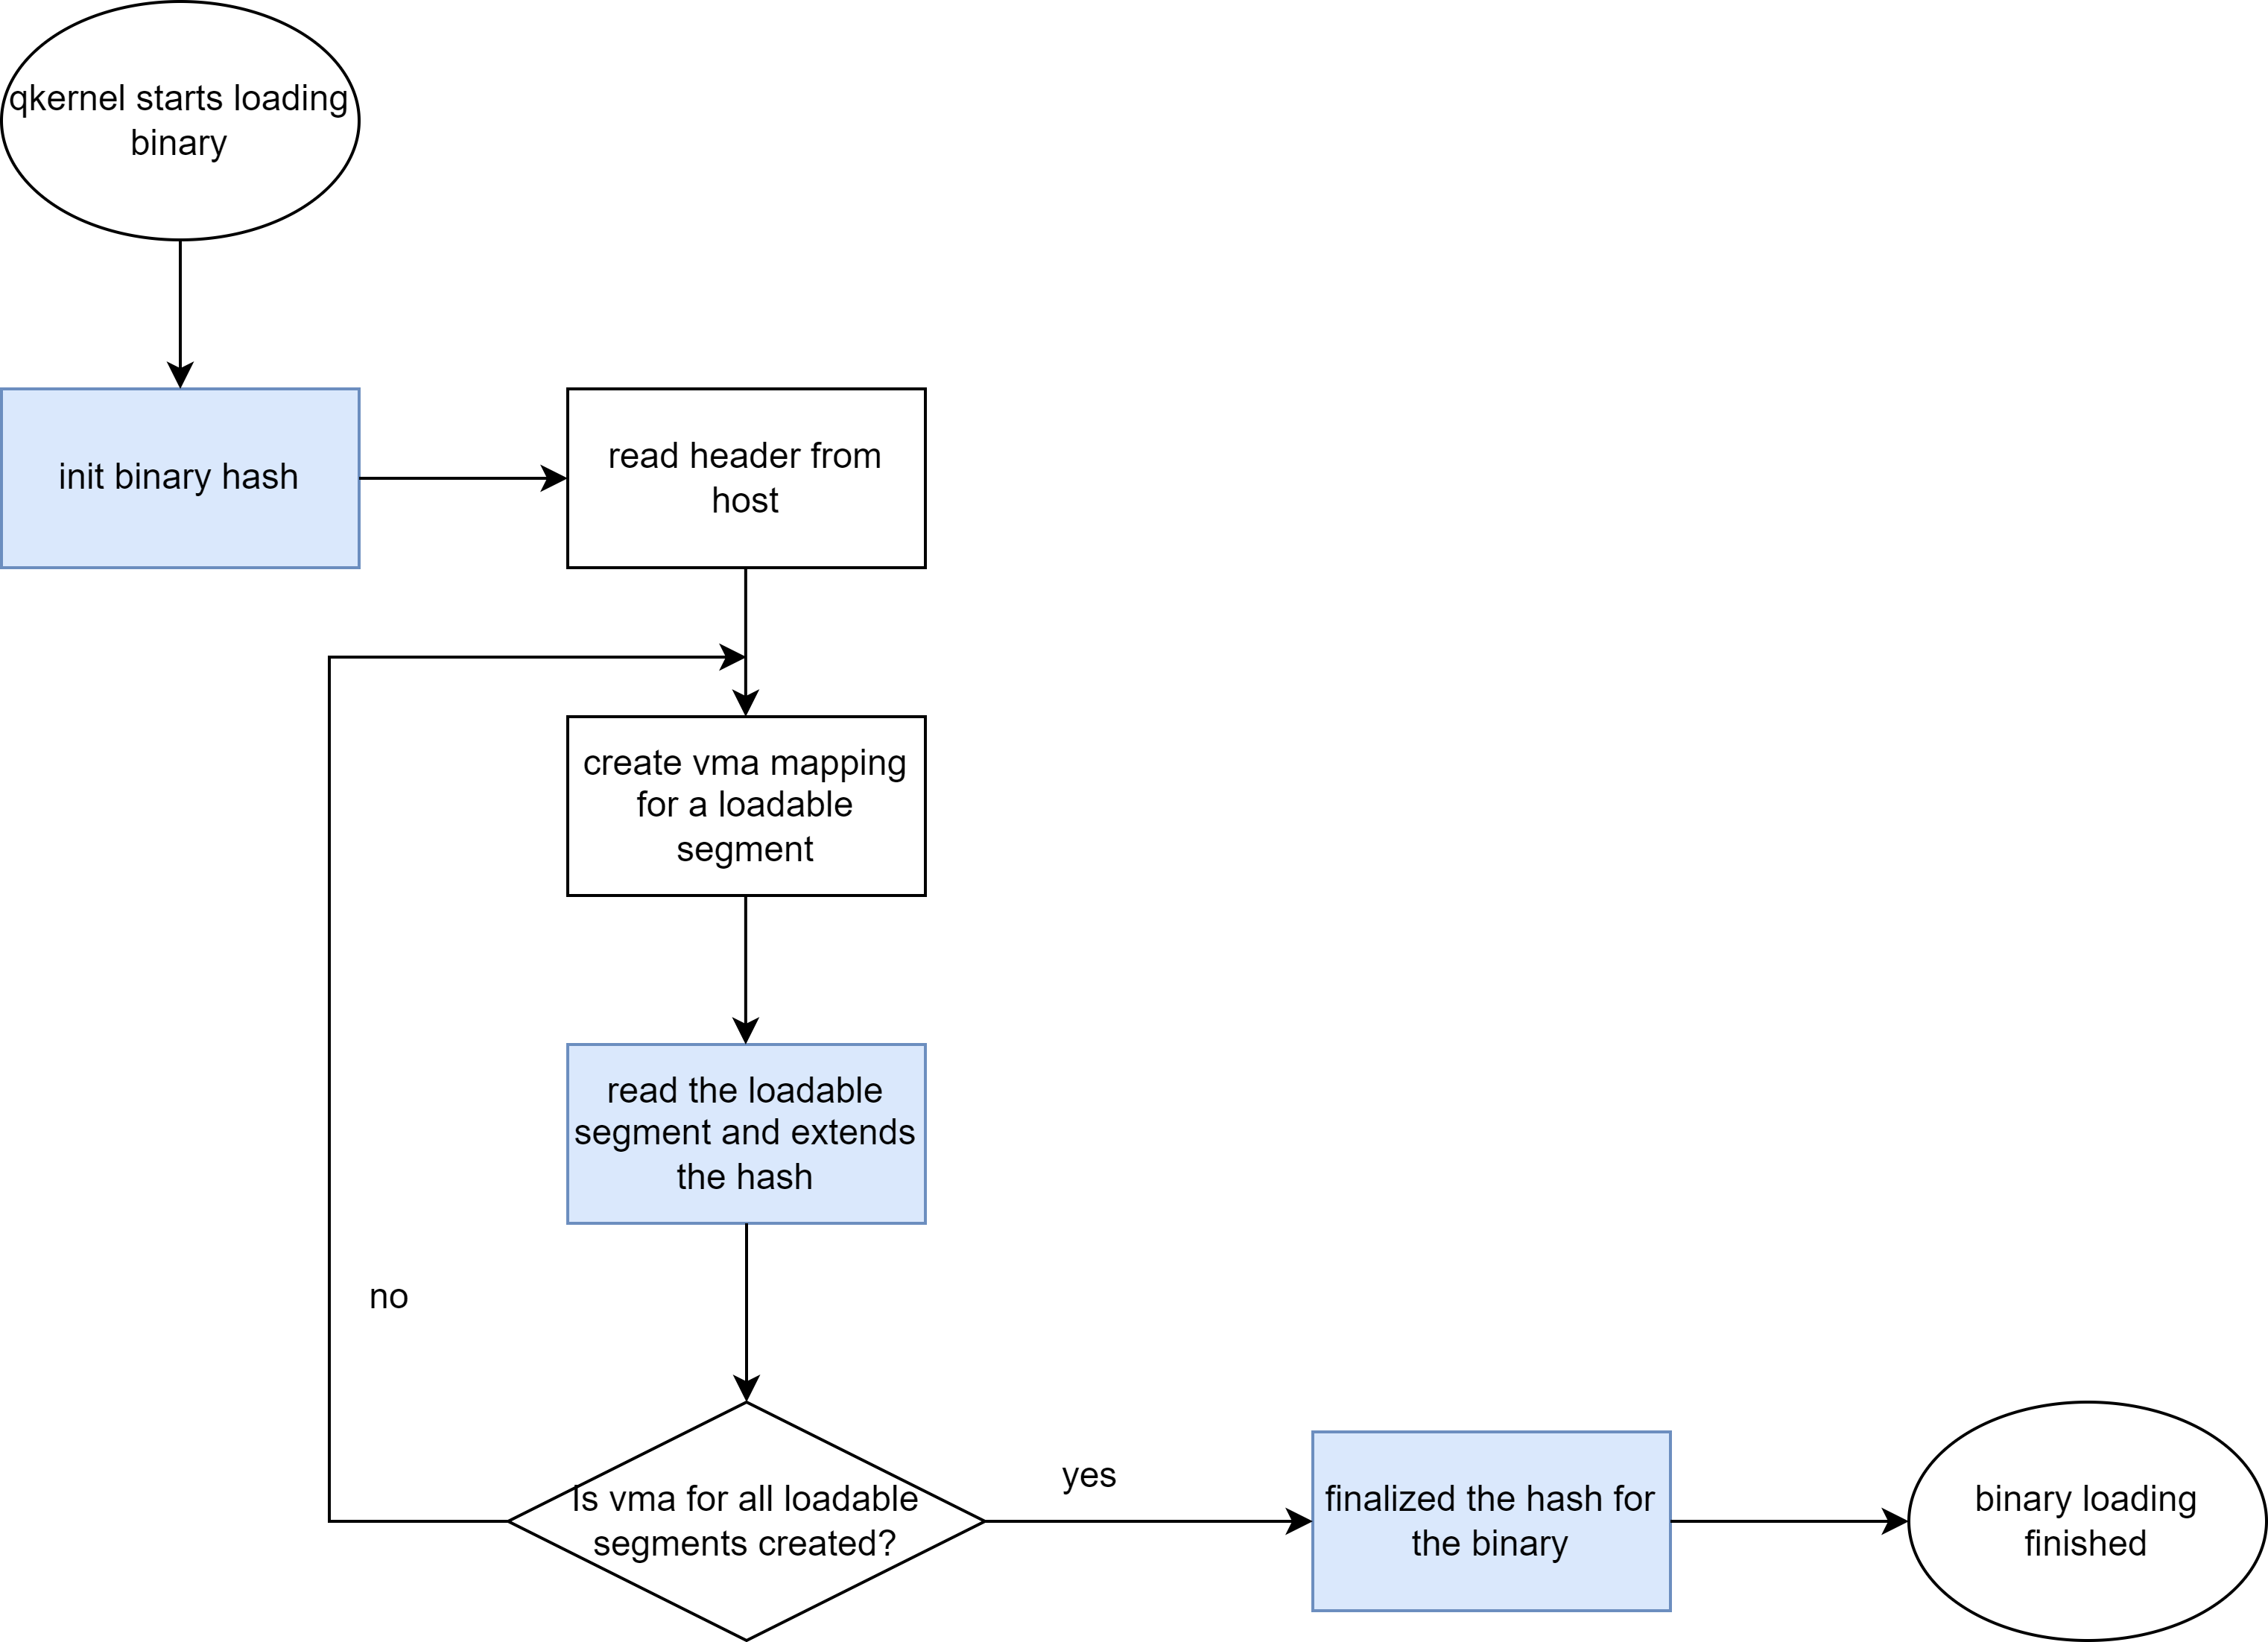
\includegraphics[width=0.8\textwidth]{images/measure_binary.png}
    \caption[Binary measurement workflow]{Binary measurement workflow}
    \label{fig:binary_measurement}
\end{figure}

Figure~\ref{fig:binary_measurement} depicts the workflow of binary measurement. Before the Qkernel loader loads a binary, the manager initializes a hash and saves it in a BtreeMap. While the binary is being measured, the manager can find the hash value using the binary name and extend it. 
As discussed in Section~\ref{sec:app_binary_loading}, the loader loads a binary by reading the binary header and creating a \acrshort{VMA} for each loadable segment. After creating a \acrshort{VMA}, the manager reads the guest virtual address range of the \acrshort{VMA} and extends the binary's hash utilizing 
the data read. The read operation will trigger page fault processing, which loads the appropriate data into guest memory (refer to Section~\ref{sec:app_binary_loading}). After the loader completes the creation of \acrshort{VMA}s for all loadable segments, the manager can obtain the binary measurement 
from the BtreeMap.




\subsection{Shared Library Measurement}

The workflow for shared library measurement is depicted in Figure~\ref{fig:measure_load_shared_libarart}. When the interpreter begins to load a dynamic library, it initiates the open system call to obtain the file descriptor for the shared library. The Qkernel open system call handler processes 
the open system call and determines whether a file is a shared library by checking its suffix (i.e., .so). If so, the handler notifies the software measurement manager to initialize a hash for the shared library, which is then stored in a BtreeMap. The manager can retrieve the hash from the map 
and extend it based on the library's name.


\begin{figure}[!htb]
    \centering
    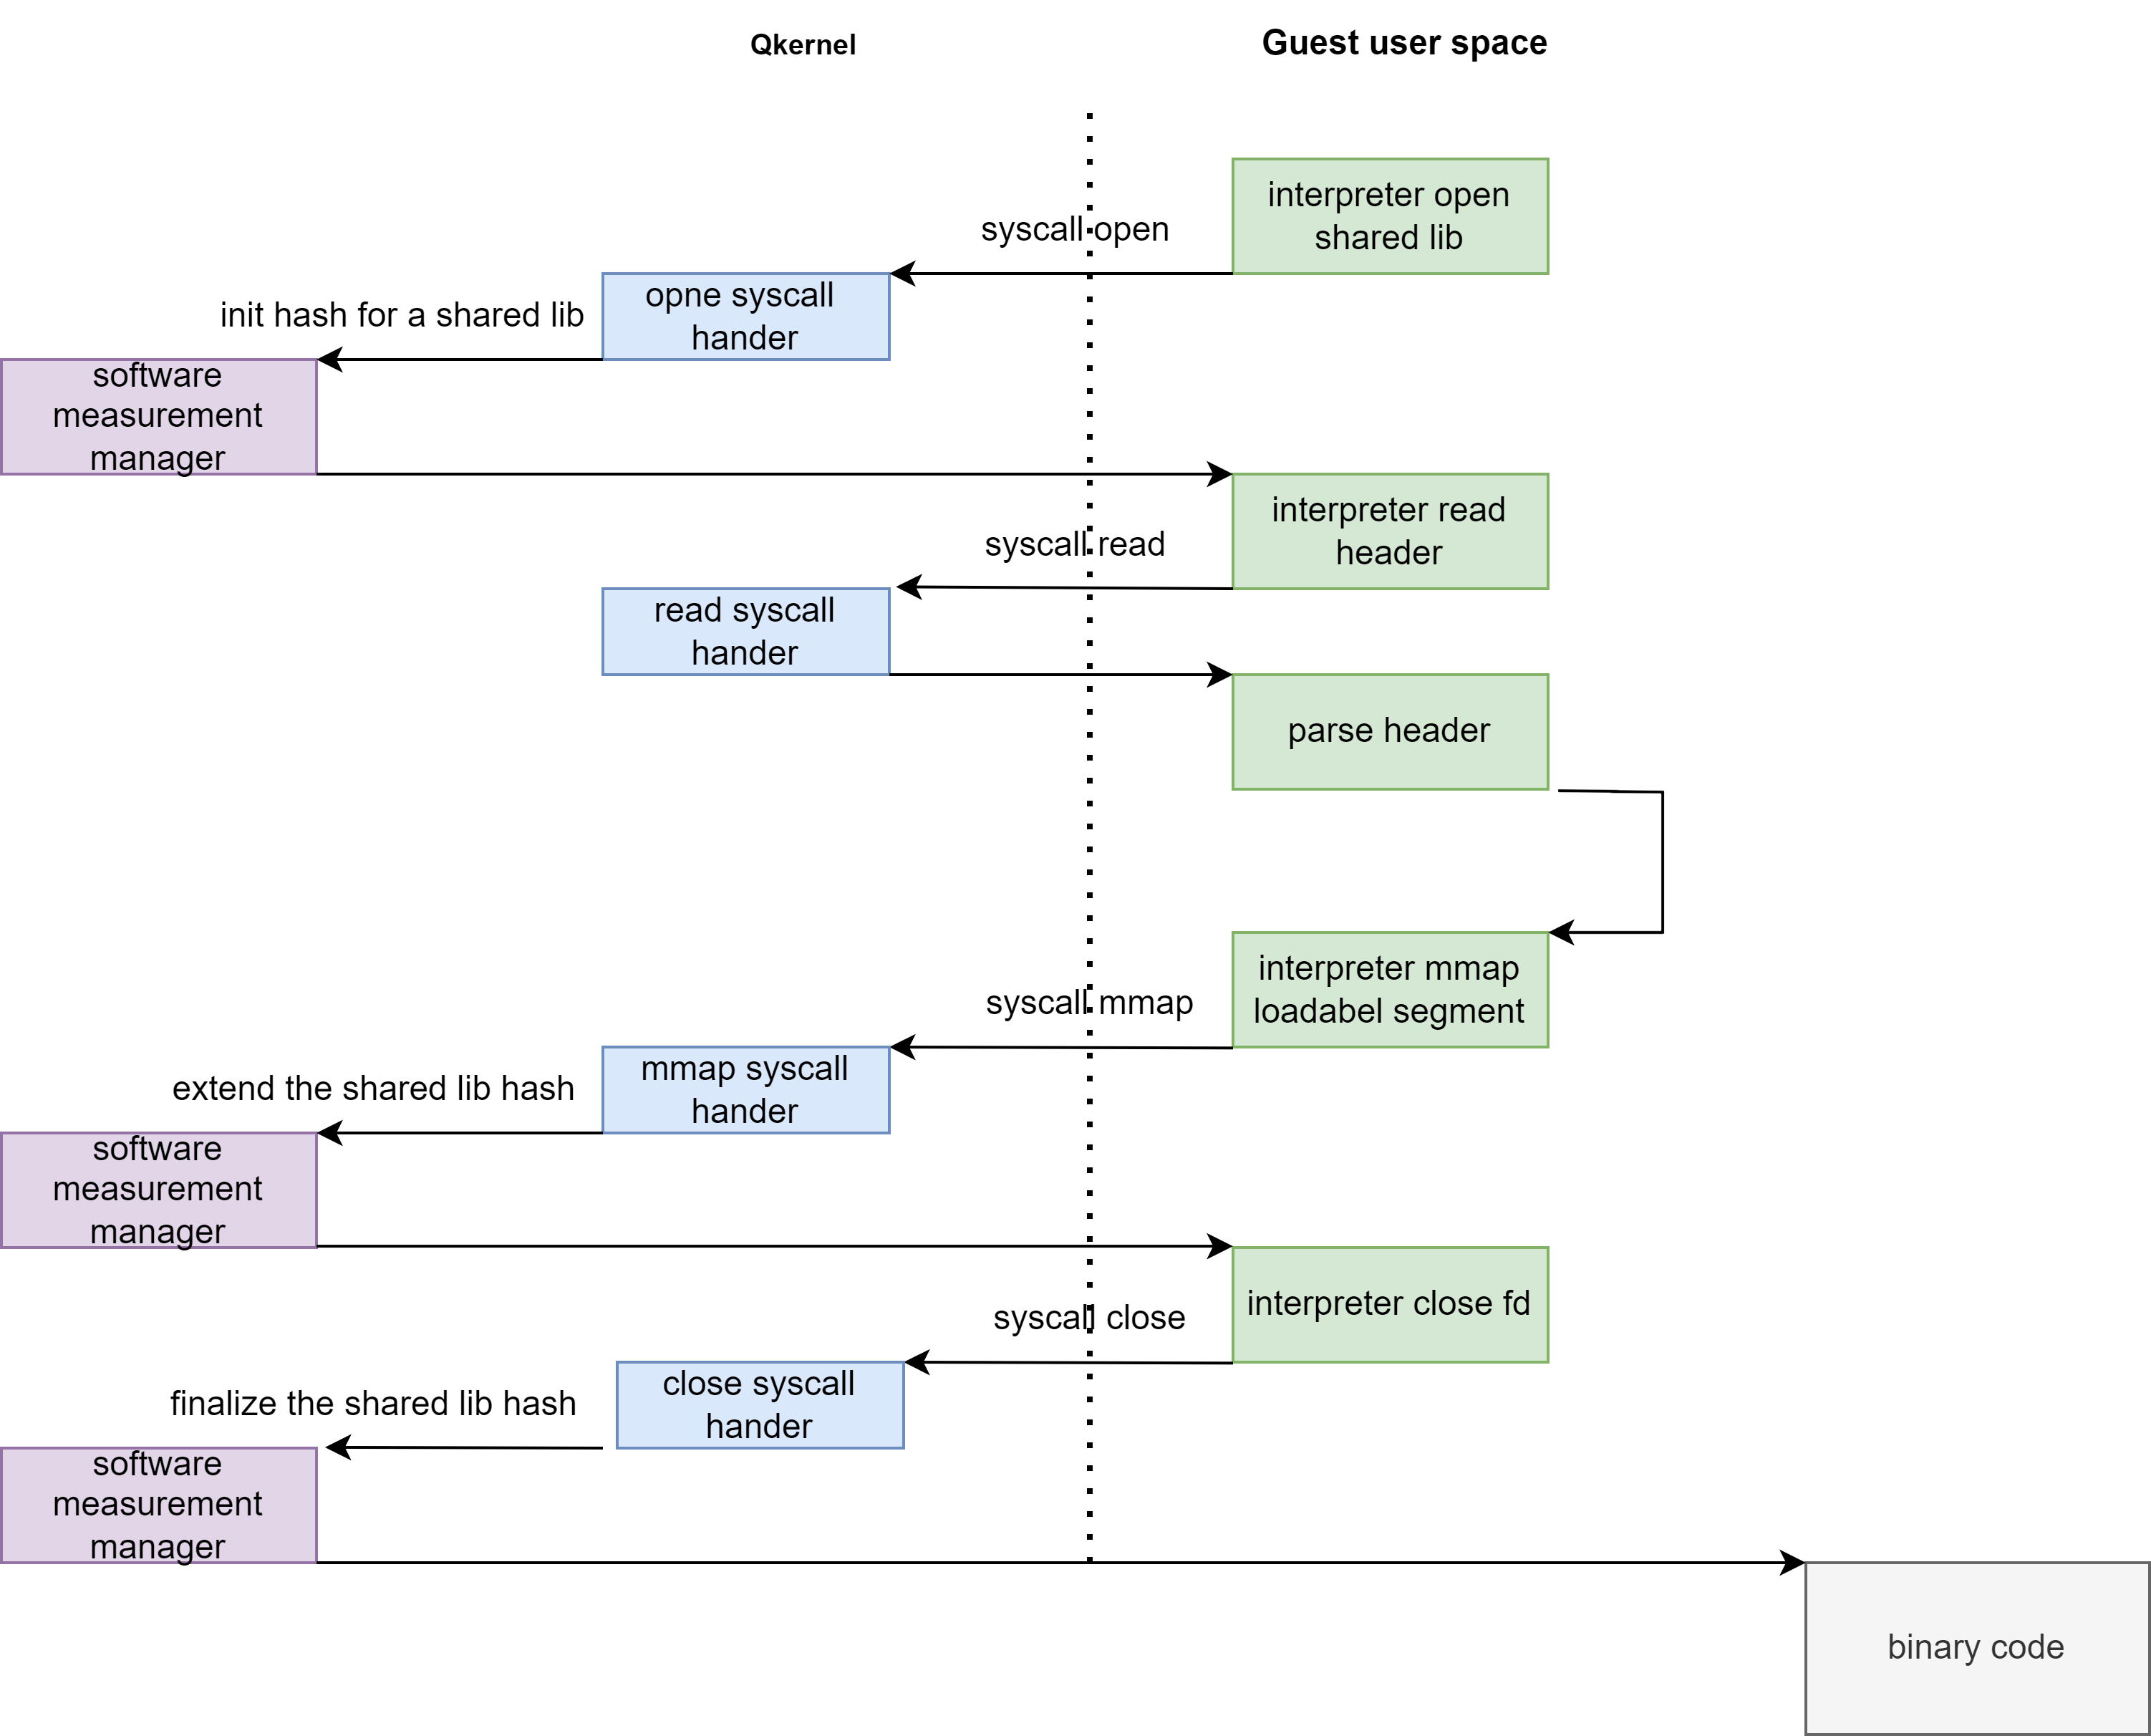
\includegraphics[width=0.8\textwidth]{images/measure_load_shared_libarart.png}
    \caption[Shared library measurement workflow]{Shared library measurement workflow}
    \label{fig:measure_load_shared_libarart}
\end{figure}

Once the open system call completes, the interpreter uses the read system call to read the library's header and find the loadable segments of the library. It then calls the mmap system call to create a \acrshort{VMA} for each segment. After the Qkernel mmap system call handler creates a \acrshort{VMA}, 
it invokes the software measurement manager. The manager will read the guest virtual memory range of the \acrshort{VMA} and extends the library's hash in the BtreeMap. As analyzed in Section~\ref{fig:measure_load_shared_libarart}, the read operation will cause the page fault handler to load the necessary data 
into the Qkernel. Since a shared library can have several loadable segments, the mmap system call can be invoked several times. The library's hash may thus be extended multiple times.


Measuring the loadable segments of a shared library is a challenge. Since the shared library is location-independent, the interpreter may map it to any location. The only requirement is that the Qkernel must make room for all the segments in their specified positions relative to the first segment. 
For this reason, the interpreter increases the mapping length to cover all the segments while mapping the first loadable segment. Because the mapping for all the segments might not be contiguous, the first \acrshort{VMA}'s virtual address range may be larger than the file size. This makes measuring the first 
segment difficult, as A KVM segment fault may be triggered if the software measurement manager reads the first \acrshort{VMA}'s address range directly. To avoid this, the software manager checks whether the \acrshort{VMA} size exceeds the file size of the shared library. If it does, the manager sets the measurement length to the 
file size of the shared library, which will cause the entire shared library to be measured. This way, the software manager can measure the first loadable segment and avoid the segment fault.



After creating the last \acrshort{VMA}, the interpreter executes the close system call to release the shared library's file descriptor. The system call handler, in turn, notifies the software measurement manager that the library loading is completed. The software measurement manager then obtains the measurement 
result of the shared library from the map. The software measurement manager will process the result differently depending on the library's loading timing, as discussed in Section~\ref{sec:Enclave_Runtime_Measurement}
\subsection{Other Measurements}
The software measurement manager uses the SHA-512 hash function. This function accepts an array of bytes and returns a hash. Since the Qkernel configuration file is a structure, the software manager first serializes it into a JSON string and then converts it into a byte array. The array will 
be used as input to the hash function to extend the enclave startup measurement. The secret manager's public key is a byte array. After the software measurement manager reads it into the enclave from the directory /usr/local/secret\_manager\_cert.pem, it can be used directly to extend the enclave 
startup hash.

\subsection{Implementation Detail}
The data structure presented in Listing~\ref{lst:shared_Lib_measurement_implementation_detail} maintained the metadata for the software measurement manager. The variables is\_app\_loaded, load\_app\_start, and load\_app\_end are employed to track the time measurements taken, i.e., enclave setup, application creation, application runtime, and application 
recreation shown in Figure~\ref{fig:soft_ware_manager_meausrment}. The manager can decide what to do with the measurements based on these three variables. The variable runtime\_binary\_reference\_measurement stores the reference measurements for the binaries and shared libraries loaded at runtime. The variable global\_measurement is a hash that can track the host data measurements since 
the enclave starts. Additionally, during program startup and restart, the manager utilizes the variables app\_binary\_ref\_measurement and restart\_binary\_measurement to track the measurement of binaries. 
Moreover, the variable shared\_lib\_measurements and binary\_measurement record the temporary hash values assigned to shared libraries and binarise during the measurement process, respectively. The manager can retrieve the corresponding hash by the file name and extend it accordingly.


\begin{lstlisting}[language=rust, caption= Interface for accessing the file type secrets, label={lst:shared_Lib_measurement_implementation_detail}]
pub struct SoftwareMeasurementManager {
    enclave_mode: EnclaveMode,
    is_app_loaded: bool,
    load_app_start: bool,
    load_app_end: bool,
    runtime_binary_reference_measurement:  BTreeMap<String, String>,
    global_measurement : String,
    enclave_ref_measurement: String,
    shared_lib_measurements: BTreeMap<String, String>,
    binary_measurement:  BTreeMap<String, String>,
    app_binary_ref_measurement : String,
    restart_bianry_measurement : String,
    startup_shared_lib_measurement_results:  BTreeMap<String, String>,
    restart_shared_lib_measurement_results:  BTreeMap<String, String>,
}
\end{lstlisting}

Since the order in which shared libraries are loaded may vary each time the application starts, the software measurement manager uses BTreeMap to record the measurement results for each shared library loaded during application startup and restart, i.e., startup\_shared\_lib\_measurement\_results 
and restart\_shared\_lib. As the Qkernel might initiate multiple processes during application startup to establish the application environment, a shared library can be loaded and measured multiple times. Therefore, when repeated measurements are made on a shared library, the manager compares 
the measurement stored in BTreeMap with the hash obtained when the library is repeatedly loaded. If there is a difference between the two, the manager will trigger a panic.


After the initial application setup, the manager generates an enclave startup hash using the measurements stored in global\_measurement and startup\_shared\_lib\_measurement\_results. This hash is stored in the variable enclave\_ref\_measurement as the enclave startup hash. The ordering of BTreeMap 
ensures that the generated enclave startup hash is consistent each time.

The application startup reference hash generally refers to the measurements stored in variable app\_binary\_ref\_measurement and startup\_shared\_lib\_measurement\_results, whereas the application restart measurements involve the measurements stored in variable restart\_binary\_measurement and 
restart\_shared\_lib\_measurement\_results. When the application is restarted, the manager first compares the app\_binary\_ref\_measurement with the restart\_binary\_measurement. This guarantees that the binaries loaded during the application restart and initial startup are identical. Subsequently, 
a comparison is made between the measurements stored in startup\_shared\_lib\_measurement\_results and restart\_shared\_lib\_measurement\_results for the shared libraries. This verification ensures that all shared libraries loaded during application restart are consistent 
with those loaded during the initial application startup.



\section{EXEC Checker}
\label{sec:impl_exec}
The EXEC checker provides the Quark agent with the API shown in Listing~\ref{lst:exec_Cheker}. This function checks EXEC requests for legitimacy and handles session allocation or policy update requests from privileged users. It returns true if the EXEC request is legitimate and false if not. 
The ExecAuthenAcCheckArgs contains the metadata required to create an EXEC process. In particular, the args in ExecAuthenAcCheckArgs is an array of strings containing the command to be executed and its arguments. If the request is privileged, the array "args" is encoded using the schema discussed in Section~\ref{sec:design_prptect_privileged_request}

\begin{lstlisting}[language=rust, caption= API of EXEC checker, label={lst:exec_Cheker}]
pub struct ExecAuthenAcCheckArgs {
    pub exec_id: String,
    pub args: Vec<String>,
    pub env: Vec<String>,
    pub cwd: String,
    pub req_type: ExecRequestType,
}
pub fn exec_req_authentication (exec_req: ExecAuthenAcCheckArgs) -> bool
\end{lstlisting}

The workflow of the function is illustrated in Figure~\ref{fig:exec_req_authentication_flow_chart}. Initially, it determines the privilege level of the request by examining whether the first element of the array "args" matches the keyword "Privileged." If it does, the function validates and decrypts the 
encrypted payload in the array. Subsequently, it verifies the legitimacy of the request's session and counter. If these components are deemed illegitimate, the function returns false. It then identifies whether the request is a session assignment or policy update request using the methods described 
in Section~\ref{subsec:design_policy_session_update}. In the case of a typical Linux command, the function checks its legality based on the policy. Specifically, it first confirms if the command is included in the command allowlist. If it is, the function checks if the directory allowlist incorporates the path-like string found in the 
command's arguments. Notably, for a no-arguments command, the function verifies if the current execution directory of the command is present in the directory allowlist. For non-privileged commands, the function only evaluates their legality based on the policy. If a command meets the policy criteria, 
the function saves the EXEC request's command and argument in plaintext. The Quark agent can then employ the EXEC ID to retrieve a legitimate EXEC request's metadata and create the corresponding process.

\begin{figure}[!htb]
    \centering
    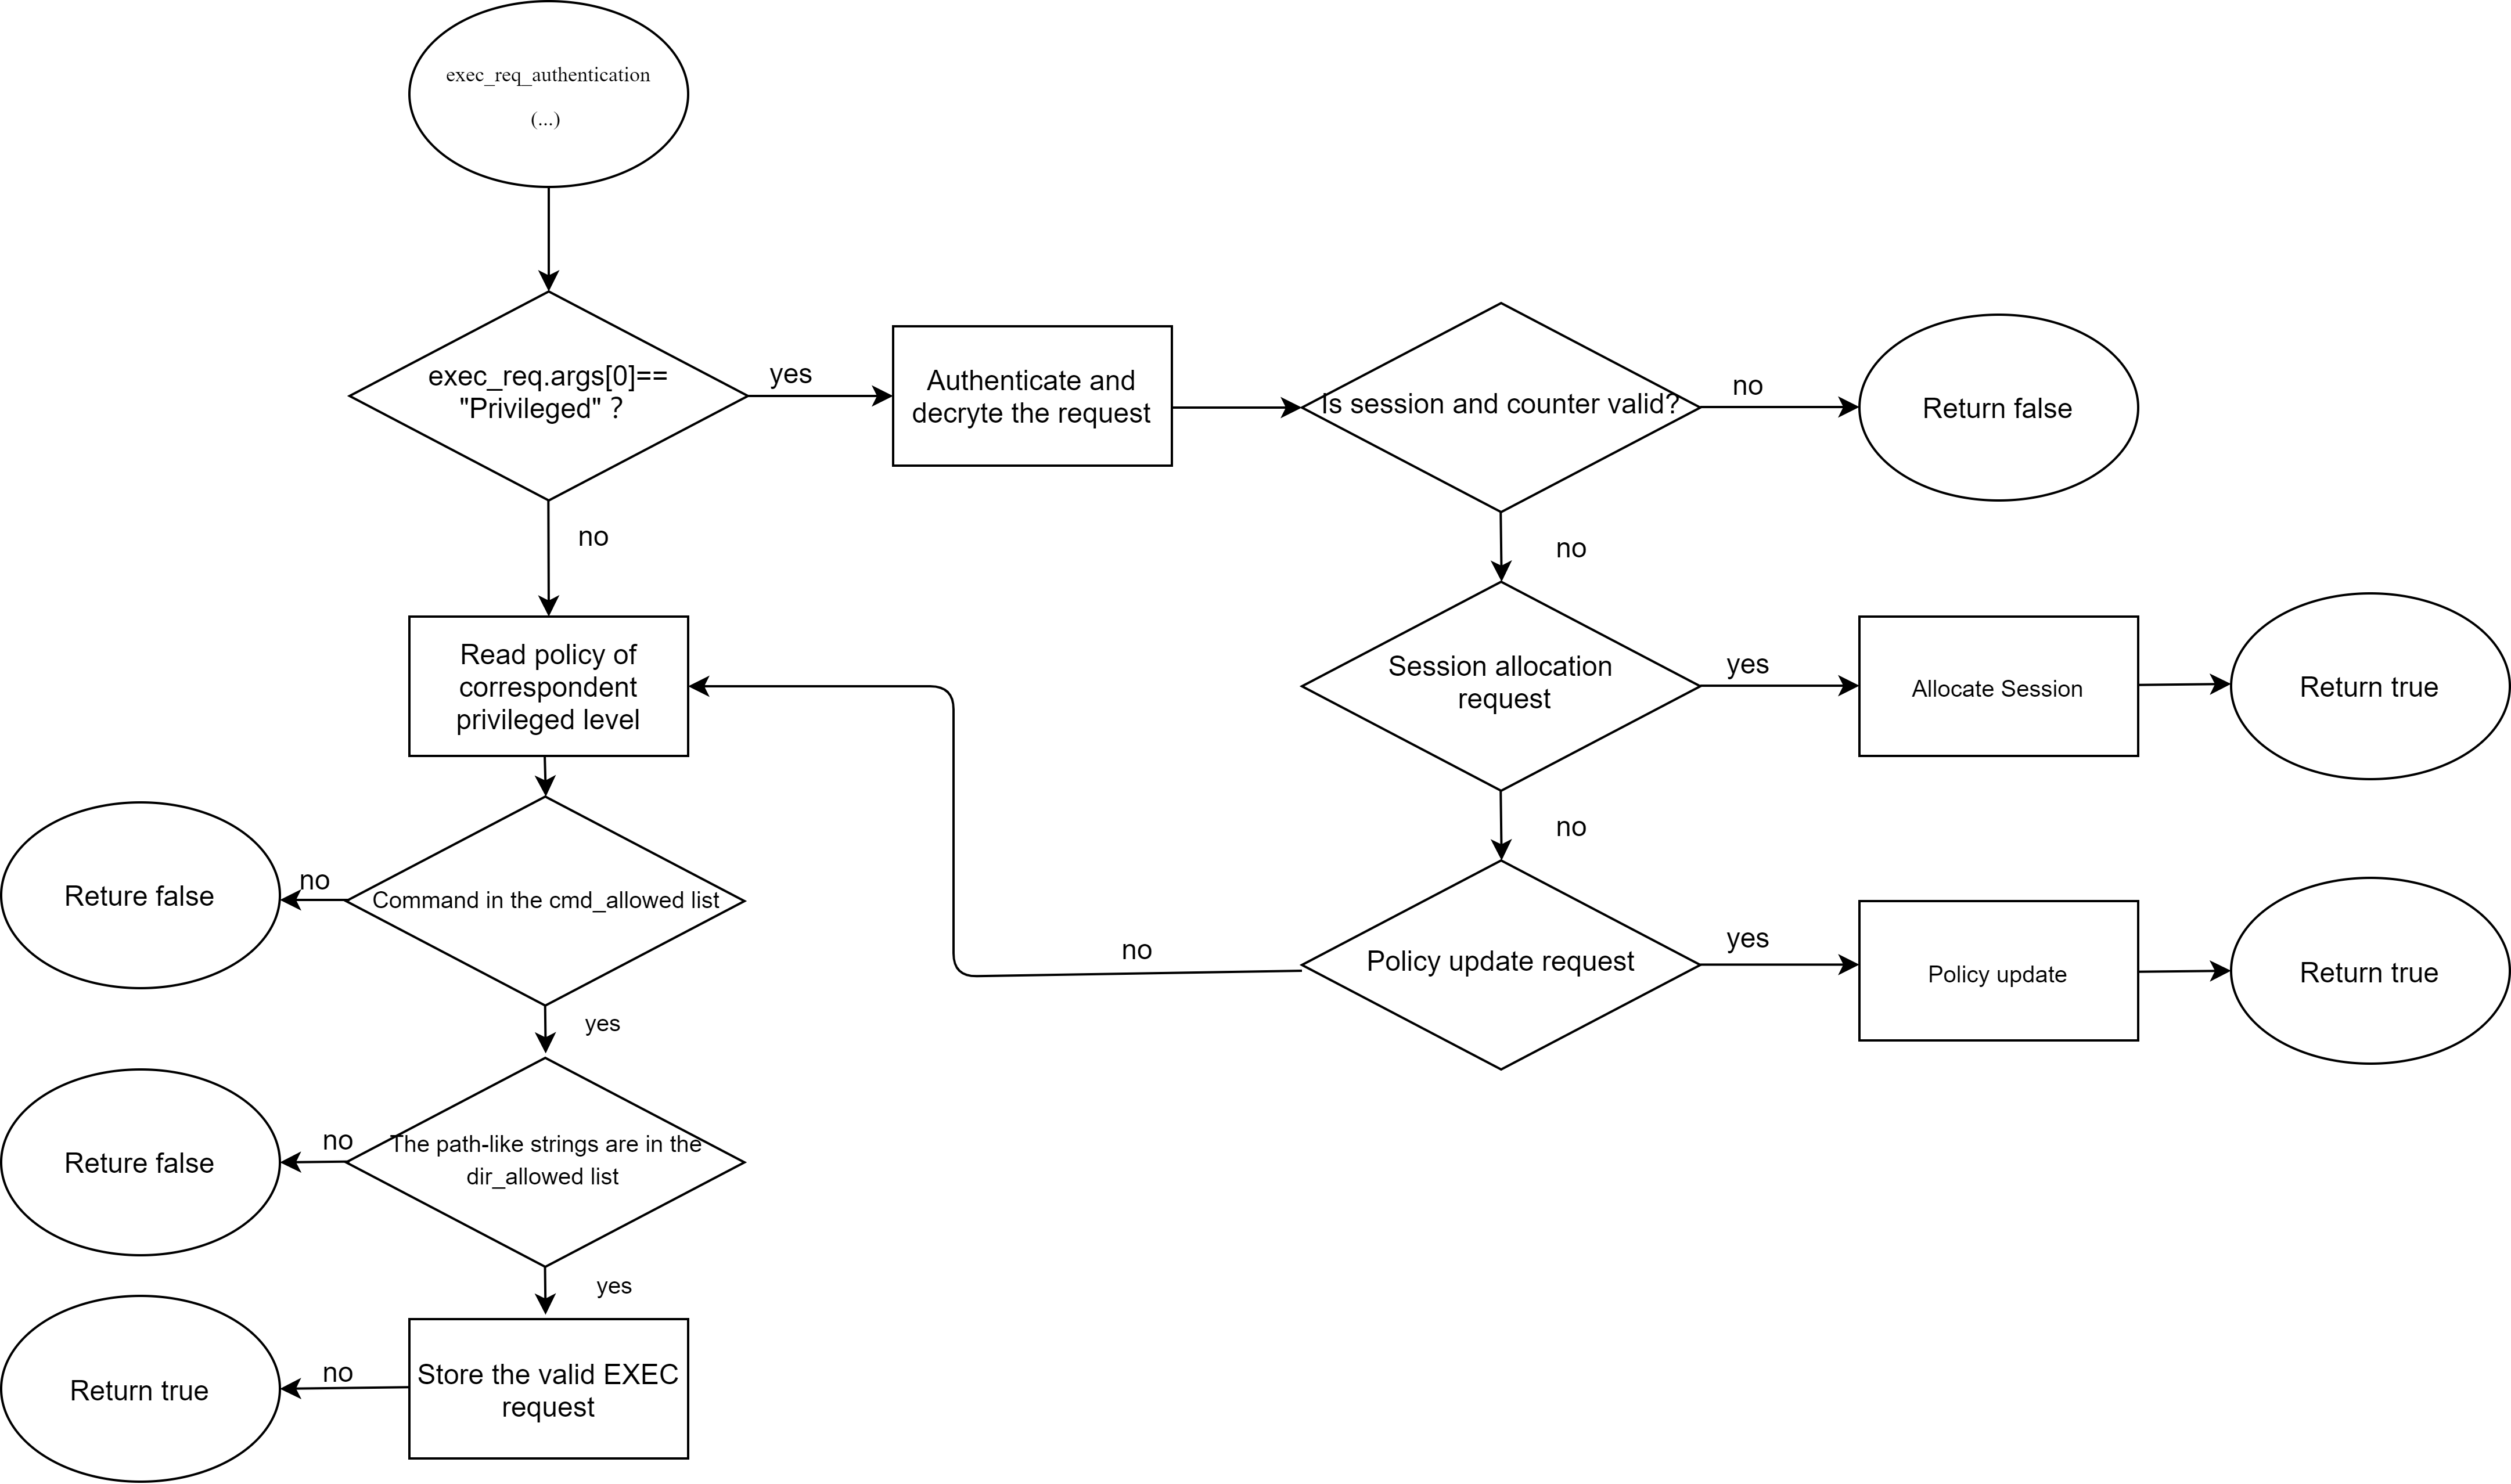
\includegraphics[width=0.8\textwidth]{images/exec_req_authentication_flow_chart.png}
    \caption[EXEC cheker workflow]{EXEC cheker workflow}
    \label{fig:exec_req_authentication_flow_chart}
\end{figure}

\section{STDIO Protection}
\label{sec:impl_STDIO}

\subsection{Inode Tracker}
The data structure InodeTracker in Listing~\ref{lst:Inode_Tracker} records information about a file descriptor that represents a process’s STDIO. It maintains a map where the key is the inode id, and the value contains metadata related to the process. 
The detail of the data structure can be found in Section~\ref{sec:design_Distinguish_io}


\begin{lstlisting}[language=rust, caption= API of Inode Tracker, label={lst:Inode_Tracker}]
pub struct InodeTracker {
    inode_track: BTreeMap<u64, TrackInodeType>,
} 
\end{lstlisting}

\subsection{Non-interactive process STDIO Protection}
\begin{lstlisting}[language=rust, caption= API of normal IO shield, label={lst:Normal_IO}]
fn encrypNormalIOStdouterr (&self, src: DataBuff, inode_id: u64) -> Result<DataBuff>
\end{lstlisting}
The function in Listing~\ref{lst:Normal_IO} encrypts STDOUT and STDERR for non-interactive processes. It accepts data written to STDOUT or STDERR and the inode id corresponding to the STDOUT or STDERR file descriptor. Depending on the enclave policy and the stored metadata in the InodeTracker, 
the function encrypts the data using the method specified in Section~\ref{sec:design_non_interactive_stdio}. Subsequently, it returns the encrypted data to Qkernel. Qkernel then sends encrypted data out via Qcall.



\subsection{Interactive process STDIO Protection}
\begin{lstlisting}[language=rust, caption= API of system call interceptor, label={lst:Termianl_IO}]
fn termianlIoEncryption(&self, src: &[IoVec], task: &Task,  inode_id: u64) -> Result<(Vec::<IoVec>)
\end{lstlisting}
Like the encrypNormalIOStdouterr function, the function in Listing~\ref{lst:Termianl_IO} is responsible for encrypting the STDOUT and STDERR of interactive processes. This not only ensures that the logs of the interactive application are encrypted but also prevents malicious 
users from attaching to the application, as discussed in Section~\ref{subsec:design_terminal}.

\section{System Call Interceptor}
\label{sec:impl_interceptor}
The three functions in the Listing~\ref{lst:Interceptor} are responsible for updating the interceptor’s policy at runtime, initializing the interceptor’s policy at enclave startup, and determining whether a system call is allowed. When the interceptor operates in ContextBased mode, 
the is\_guest\_syscall\_allowed function utilizes the application process id stored in the structure GuestSyscallInterceptor to identify whether a process is the application process. To prevent competition between the three functions accessing the interceptor's policy, the interceptor is 
protected by RwLock. Additionally, the BackEndSyscallInterceptorConfig maintains a vector that contains the id of allowed system calls (allowlist). The is\_guest\_syscall\_allowed function checks whether a system call's ID is present in this list to determine whether the system call is allowed. 
It is important to note that accessing this allowlist has an O(n) time complexity.

\begin{lstlisting}[language=rust, caption= API of system call interceptor, label={lst:Interceptor}]
static ref SYSCALLINTERCEPTOR:  RwLock<GuestSyscallInterceptor> = RwLock::new(GuestSyscallInterceptor::default());

pub struct BackEndSyscallInterceptorConfig {
    pub syscalls: Vec<u64>
…
}

pub struct GuestSyscallInterceptor {
    policy: BackEndSyscallInterceptorConfig,
    application_pid: i32,
}

pub fn syscall_interceptor_policy_update(policy: &BackEndSyscallInterceptorConfig) -> Result<()> 
pub fn syscall_interceptor_init(policy: BackEndSyscallInterceptorConfig) -> Result<()> 
pub fn is_guest_syscall_allowed(current_pid: i32, syscall_id: u64) -> bool
    
\end{lstlisting}


\section{Qlog Manager}
\label{sec:iml_qlog}
Listing~\ref{lst:Qlog} presents the API of the Qkernel log manager. The QlogManager structure maintains the Qlog manager's policy, as shown in Figure~\ref{fig:qkernel_Log_config}. The shielding layer uses the function  qlog\_manager\_init to initialize or update the policy. 
The function is\_log\_level\_allowed  is invoked by 
the Qkernel logging system. It accepts the level of the log that currently needs to be printed. It returns true if the log level is the same or less than the log level specified in the policy. If this function returns false, the Qkernel logging system will not print the log message.

\begin{lstlisting}[language=rust, caption= API of Qlog manager, label={lst:Qlog}]
pub struct QlogManager {
    policy: QlogPolicy,
}
pub fn is_log_level_allowed(current_log_level: QkernelDebugLevel) -> bool
pub fn qlog_magager_init()   
\end{lstlisting}


\section{Summary}
In this chapter, we explain how the design in Chapter~\ref{sec:design} was implemented. In the next chapter, we evaluate the performance and security of the system.


\cleardoublepage



%%% Local Variables:
%%% TeX-master: "diplom"
%%% End:


\chapter{ZUSAMMENFASSUNG UND WERTUNG}
\label{sec:evaluation}

Die Simulationsergebnisse können beweisen, dass die Entwurfsziele erreicht wurden. Die gewählte Architektur ermöglicht es, den Algorithmus schnell und effizient zu implementieren. Darüber hinaus wird der Hardwareaufwand minimiert und effektiv genutzt.

\vspace{\baselineskip}

\noindent Es ist wichtig zu beachten, dass die Eingaben in der Simulation nicht dezimal, sondern hexadezimal sind. Die Addition und der Speicher sollten entsprechend den Anforderungen ausgewählt werden, und es sollte ein geeignetes Modell gewählt werden. Wir verwenden hier einen 64-Bit-Addition.

\vspace{\baselineskip}

\noindent Diese Entwurfsarbeit hat mir eine allgemeine Übersicht darüber verschafft, wozu ich als Entwickler in der Lage sein sollte. Ein Entwickler muss die Hardware-Implementierung schon zu Beginn des Entwurfs berücksichtigen. Bei meinem ersten Design traten Probleme bei der Simulation auf, und ich habe viele Veränderungen vorgenommen, bevor ich es erfolgreich umsetzen konnte.

\vspace{\baselineskip}

\noindent Ich möchte mich auch bei meinem Praktikumsbetreuer bedanken. Er stand mir immer zur Verfügung, um meine Fragen zu beantworten und mir Anregungen zu geben, die mir halfen, meinen Entwurf schneller fertigzustellen.
\cleardoublepage


%\input{content/60_futurework.tex}

\appendix
\chapter{Conclusion And Outlook}
\label{sec:conclusion}

%  Schlußfolgerungen, Fragen, Ausblicke

% Dieses Kapitel ist sicherlich das am Schwierigsten zu schreibende. Es
% dient einer gerafften Zusammenfassung dessen, was man gelernt hat. Es
% ist möglicherweise gespickt von Rückwärtsverweisen in den Text, um dem
% faulen aber interessierten Leser (der Regelfall) doch noch einmal die
% Chance zu geben, sich etwas fundierter weiterzubilden. Manche guten
% Arbeiten werfen mehr Probleme auf als sie lösen. Dies darf man ruhig
% zugeben und diskutieren. Man kann gegebenenfalls auch schreiben, was
% man in dieser Sache noch zu tun gedenkt oder den Nachfolgern ein paar
% Tips geben. Aber man sollte nicht um jeden Preis Fragen, die gar nicht
% da sind, mit Gewalt aufbringen und dem Leser suggerieren, wie
% weitsichtig man doch ist. Dieses Kapitel muß kurz sein, damit es
% gelesen wird.

% \ldots conclusion \ldots

% \todo{write conclusion}

This thesis aims at enabling untrustworthy cloud providers to orchestrate applications within \acrshort{CVM} while ensuring the confidentiality and integrity of applications' data. In particular, to minimize the \acrshort{TCB} of the CVM, \acrshort{pVM} is selected as a starting point.
 
Chapter~\ref{sec:security_analyse} analyzes the security risks of the OCI runtime interface. To address these concerns, the thesis introduces the OCI runtime interface shield and proposes modifications to the OCI runtime interface in Chapter~\ref{sec:design}. The shield is implemented 
within the \acrshort{CVM} and enforces a policy provided by the application owner on the OCI interface. Figure~\ref{fig:generic_policy} illustrates an example of such a policy. The shield allows the application owner to remotely verify the state of the \acrshort{CVM} and securely deploy secrets. 
While the \acrshort{CVM} is operational, the shield can authenticate and do access control on EXEC requests, encrypts STDIO for the processes running in the \acrshort{CVM}, restricts guest system calls, and manages \acrshort{CVM} logs. Additionally, a secure client for the application owners is 
implemented, enabling them to issue privilege commands and update the shield policy.
 
The qualitative analysis in Section~\ref{sec:eva_qualitativ} proves that the system implemented in Chapter~\ref{sec:implementation} can effectively mitigate most issues found in security analysis. A summary of the analysis can be found in Table~\ref{tab:eva_qualitativ_summary}. 
On the other hand, the quantitative analysis in Section~\ref{sec:eva_Quantitative} reveals performance degradation due to the system. This is evident in longer application startup time, 
decreased application throughput, an increased \acrshort{TCB} size, etc. Nevertheless, Quark's \acrshort{TCB} is only one-sixteenth the size of Kata Containers\cite*{Kata-Containers}, highlighting the superiority of the \acrshort{pVM} architecture. 
 
Further work is required before the solution can be deployed. For example, support for running Quark on secure VMs (e.g., Intel TDX~\cite*{Intel_tdx_whitepaper}) and enhancing the remote attestation infrastructure are necessary. The following section provides a detailed discussion of these aspects.


\section{Furture Work}

Chapter~\ref{sec:design} provides solutions to the problems identified through the security analysis in Chapter~\ref{sec:security_analyse}. However, some of these were not implemented since they were out of scope. This includes the secret uploading discussed in 
Section~\ref{sec:design_Secret_Uploading}, the methods to mitigate secret cross-leakage described in Section~\ref{sec:secure_application_deployment} on page \pageref{eq:1}, and the terminal protection outlined in Section~\ref{subsec:design_terminal}. In the next step, the 
priority will be to implement these designs.

Currently, the secret manager operates locally and utilizes a local file system backend to store secrets. However, in the future, the goal is for the secret manager to run in the cloud and manage secrets from multiple stakeholders. Thus, it is necessary to place the secret manager in 
a secure virtual machine and develop a confidential backend. The backend can be memory-based or storage-based. The former is more straightforward because the VM's memory is encrypted. On the other hand, if the latter option is chosen, it is essential to 
incorporate a file system shielding layer~\cite*{file_system_shield} to prevent any leakage of secrets written to the VOLUME.

The remote attestation infrastructure is immature, as Quark can only generate simulated attestation reports. As discussed in Section~\ref{subsec:Limitations}, in this case, the secret manager cannot verify the report's authenticity. Future implementations will have to close this security 
gap.

The performance evaluation in Section~\ref{bench_Interceptor} shows that the guest system interceptor imposes a significant latency overhead. As discussed in Section~\ref{sec:impl_interceptor}, these overheads arise from accessing the vector that holds the system calls whitelist and the lock 
that safeguards the vector. In future implementations, a possible solution could involve storing the system call whitelist in eight \texttt{AtomicU64}~\cite*{rust_automic_u64} variables, with each bit in the variable representing a system call ID. Given that Quark consists of a total of 451 system calls, eight variables would suffice. The whitelist can then be accessed using atomic 
operations to circumvent the previously mentioned overhead.

Quark lacks protection for the VM's memory and registers states. Thus, untrusted entities (e.g., virtual machine hypervisors) can gain access to secrets stored within the VM. To tackle this issue, the future implementation must modify Quark's architecture to support either 
AMD SEV SNP~\cite*{SEV_SNP_white_book} or Intel TDX~\cite*{Intel_tdx_whitepaper}.

Quark uses a parevirtualized file system sharing mechanism to share files and volumes stored on the host with applications on the guest. Any changes made to the files by the application are reflected on the host. This poses a security risk because an attacker can access an application's secrets by 
accessing the rootfs of the application on the host. A common approach is implementing a guest filesystem shield to protect inbound and outbound guest data. Those interested in learning more about this topic should refer to~\cite*{file_system_shield}.

Quark lacks authentication to network requests and cryptographic protection for transmitted data, resulting in potential unauthorized access to the application or man-in-the-middle attack~\cite*{Man_in_the_middle_attack}. For instance, attackers can use \emph{kubectl port-forwarding} to connect to an 
application listening on the target port and acquire the application's confidential data or service. A possible solution is implementing a guest network shield that leverages TLS\cite*{tls_record_size} to authorize incoming network requests and provides cryptographic protection for incoming and 
outgoing data. However, this thesis does not cover this type of vulnerability, and readers are encouraged to refer to~\cite*{network_shiled}.

Currently, a \acrshort{CVM} is restricted to running a single application. Attempting to load additional applications into the \acrshort{CVM}  will cause the software measurement manager to panic since the application restart hash does not match the application startup reference hash. 
This prevents the service mesh from working properly since it requires the sidecar container to be run in the \acrshort{CVM}. As such,  future releases should involve an extension of the software measurement manager. In this case, the application owner can specify the loadable containers and their 
reference hashes in the shield policy. This will allow the \acrshort{CVM} to load additional containers. During the loading process, the software measurer will use the container's reference hash to ensure that the loaded container binaries are correct.




\cleardoublepage

%%% Local Variables:
%%% TeX-master: "diplom"
%%% End:



% \printglossary[type=\acronymtype]

% \addchap{Glossar}

% makeglossaries diplom
% \printglossary[style=altlist]
\printglossary[type=\acronymtype,style=long]


\printbibliography
\iffalse
    % an aid for Kile autocompletion
    \bibliography{own.bib}
\fi

\end{document}